\documentclass{dissertation}

\usepackage{tabularx}
\usepackage{longtable}
% \usepackage{amssymb,amsmath}
% \usepackage{capa}
% \usepackage[sort&compress,authoryear]{natbib} % Para usar estilo novo de refer�ncias
% \usepackage{verbatim}
% \usepackage{enumerate}
% \usepackage{colortbl}
% \usepackage{color}
% \usepackage{textfit}




\graduationsecretary{SERVI�O DE P�S-GRADUA��O DO ICMC-USP}
\advisor{Prof�. Dr�. Renata Pontin de Mattos Fortes}
\address{S�o Carlos - SP}
\author{D�bora Maria Barroso Paiva}
\title{Um processo envolvendo elementos de \textit{design rationale} para projetos de pesquisa em software}
\depositshortdate{Maio de 2007}
\depositfulldate{10.05.2007}
\defenseshortdate{10.05.2007}
\defensefulldate{10.05.2007}
\dissertationgoal{Tese apresentada ao Instituto de Ci�ncias Matem�ticas
e de Computa��o -- ICMC-USP, como parte dos requisitos para
obten��o do t�tulo de Doutor em Ci�ncias -- Ci�ncias de Computa��o
e Matem�tica Computacional.}



\begin{document}

\frontmatter

% \maketitle

%%%%%%%%%%%%%% Agradecimentos %%%%%%%%%%%%%%%%%

{\huge{\textbf{Dedicat�ria}}}

\rule{\linewidth}{2pt} \vspace{14cm}


\begin{flushright}
\textit{Aos meus pais Moacir e Maria Helena, por terem }

\textit{me dado a luz da vida e amor incondicional.}

\textit{Aos meus irm�os Karina e Hugo, pela valiosa amizade.}

%\textit{Ao meu orientador Rudinei, pela oportunidade de chegar a este momento.}

\textit{Aos meus amigos, por terem colaborado}

\textit{com minha forma��o pessoal e profissional.}

%\textit{e � minha esposa Taciana, pelo seu amor e apoio incondicionais.}
\end{flushright}


%
%\begin{flushright}
%\textit{Aos meus pais Lu�s e Ilca, por terem me dado a luz da vida;}
%
%\textit{�s minhas irm�s Renatha e Roberta, por me darem for�a para lutar;}
%
%\textit{ao meu futuro sobrinho, que rezo para nascer com sa�de;}
%
%\textit{� minha orientadora Gra�a, pela oportunidade de chegar a este momento;}
%
%\textit{aos meus amigos, por terem colaborado com minha forma��o;}
%
%\textit{e � minha esposa Taciana, pelo seu amor e apoio incondicionais.}
%\end{flushright}

\chapter*{\centering{Agradecimentos}}

\rule{\linewidth}{2pt} \vspace{0.2cm}

A Deus, por iluminar o meu caminho.

� minha m�e, por seu amor incondicional, por ter me ensinado a batalhar pelos sonhos e a ser forte perante as dificuldades.  

� minha irm� pela amizade, pelo imenso amor que tem por mim, pelo companheirismo e por me apoiar sempre.

Aos meus irm�os, pelo carinho.

� minha orientadora, professora Dra. Renata Pontin de Mattos Fortes, pelos ensinamentos, pelas partilhas e, sobretudo, pela amizade e pela confian�a que depositou em mim como sua primeira aluna de doutorado. 

� professora Dra. Rosely Sanches pelas in�meras e valiosas contribui��es durante o desenvolvimento do trabalho, pelo carinho e por transmitir uma energia t�o positiva.

Ao professor Dr. Jos� Carlos Maldonado, pelas excelentes sugest�es e cr�ticas em rela��o ao trabalho, pela disponibilidade em colaborar e pela amizade.  

Aos meus familiares que sempre me incentivaram e apoiaram.  

Aos v�rios amigos e colegas, pessoas muito especiais, com as quais convivi nesse per�odo. Aprendi muito com voc�s! Obrigada por terem ajudado a renovar a esperan�a nos momentos dif�ceis e por terem compartilhado os momentos alegres. 

A todos que fizeram e fazem parte do grupo de pesquisa, pela amizade, pelas discuss�es e trocas de experi�ncias t�o enriquecedoras. Em especial ao Andr� Pimenta Freire, pelas expressivas contribui��es. 

Aos professores, funcion�rios e estudantes do Departamento de Computa��o e Estat�stica da Universidade Federal de Mato Grosso do Sul, por terem me recebido com tanto carinho.

A todos aqueles que participaram dos estudos de caso realizados, pelas importantes contribui��es.

Ao ICMC-USP pela oportunidade e � CAPES pelo aux�lio financeiro.




\begin{resumo}
%{\huge{\textbf{Resumo}}}

%\hspace{-0.5cm}\rule{\linewidth}{2pt}

%\vspace{3cm}

%\chapter*{\centering{Resumo}}

%\ renata -- Debora, acho que o resumo est� muito sucinto, assim eu dei algumas sugestoes de melhor contextualizar.... inclui as linhas iniciais para falar de processos pois a definicao de processos nem sempre � obvia para os leitores, dai achei melhor dizer que os processos sao os relacionados com a engenharia de software.. uma definicao de processo que acho bem popular � a da wikipeadia: Na ci�ncia da computa��o, processo pode ter v�rios significados:  * Na Engenharia de Software, processo � um conjunto de passos parcialmente ordenados, cujo objetivo � atingir uma meta: entregar um produto de software de maneira eficiente, previs�vel e que atinja as necessidades de neg�cio. Geralmente inclui an�lise de requisitos, programa��o, testes, entre outras tarefas.  Ver tamb�m: processos da ger�ncia de projetos.  * Em Sistemas Operacionais, processo � um m�dulo execut�vel �nico, que corre concorrentemente com outros m�dulos execut�veis. Por exemplo, em um ambiente multi-tarefa (como o Unix) que suporta processos, um processador de texto, um navegador e um sistema de banco de dados s�o processos separados que podem rodar concomitantemente.  ****** Debora, tambem achei que  voce foi muito resumida com relacao a TUDO que voce fez... os levantamentos, e estudos de caso, mas, voce acha que deve ser mesmo bem conciso o resumo?? Ah, porque eu nao sei se os leitores sabem sobre design rationale, eu coloquei um inicio sobre isso ta?

O volume crescente de projetos de pesquisa que envolvem software motiva a realiza��o de an�lises sobre os processos utilizados no desenvolvimento desses projetos, considerando-se as atividades cumpridas, os resultados obtidos e a aplica��o de recursos. Na �rea de Engenharia de Software, processos t�m sido propostos nos �ltimos anos com o objetivo de contribuir para o desenvolvimento de projetos de pesquisa que envolvem software.
Busca-se, de forma geral, auxiliar o gerenciamento dos diversos artefatos que podem ser gerados, por exemplo, modelos, c�digo fonte, relat�rios t�cnicos e artigos cient�ficos. As solu��es apresentadas na literatura come�aram a ser propostas recentemente e, portanto, os estudos realizados nessa �rea apresentam-se em est�gio bastante inicial. %Observa-se que as solu��es cobrem parcialmente um conjunto de requisitos referentes a processos para desenvolvimento de projetos de pesquisas. 
Dessa forma, o objetivo deste trabalho foi definir um processo para o desenvolvimento de projetos de pesquisa envolvendo software, que esteja de acordo com um conjunto de requisitos identificado e que possa contribuir para a evolu��o desses projetos. Para refor�ar a continuidade dos projetos, foi estudada a abordagem de {\it design rationale}, com o objetivo de oferecer meios para que as decis�es de projeto sejam capturadas e registradas em fases espec�ficas do desenvolvimento. O processo de documenta��o foi enfatizado, ou seja, foi investigado como a abordagem de {\it design rationale} poderia ser utilizada para melhorar a documenta��o dos projetos de pesquisa. Como um resultado obtido, um modelo para representa��o de {\it design rationale} foi definido, implementado em uma ferramenta CASE e avaliado em um experimento.

%\anterior, da debora:
%Processos t�m sido propostos nos �ltimos anos com o objetivo de contribuir para o desenvolvimento de projetos de pesquisa que envolvem software. A principal motiva��o � auxiliar o gerenciamento dos diversos artefatos que podem ser gerados, por exemplo, modelos, c�digo fonte, relat�rios t�cnicos e artigos cient�ficos. As solu��es apresentadas na literatura come�aram a ser propostas recentemente e, dessa forma, os estudos realizados nessa �rea apresentam-se em est�gio bastante inicial. Com isso, p�de ser observado que as solu��es cobrem parcialmente um conjunto de requisitos referentes a processos para desenvolvimento de projetos de pesquisas que foi identificado. O objetivo deste trabalho foi, portanto, definir um processo para desenvolvimento de projetos de pesquisa envolvendo software que possa contribuir para a evolu��o desses projetos. O processo de documenta��o foi enfatizado, ou seja, foi investigado como a abordagem de {\it design rationale} poderia ser utilizada para melhorar a documenta��o dos projetos de pesquisa. Como resultado, foi obtido um modelo para representa��o de {\it design rationale}, que foi implementado em uma ferramenta CASE e avaliado em um experimento.   
 
 %l�m disso, observou-se, a partir de relaos apresentados na literatura, que muitos pesquisadores t�m dificuldades em dar continuidade aos projetos de pesquisa, devido a fraca motiva��o para a atividade de documenta��o. Assim, 
\end{resumo}

\begin{abstract}
\chapter*{Abstract}
\thispagestyle{empty}

% \addcontentsline{toc}{section}{Abstract}

\versal{T}he task of term extraction in textual domains, which is a subtask of the text pre-processing in Text Mining, can be used for many purposes in knowledge extraction processes. These terms must be carefully extracted since their quality will have a high impact in the results. In this work, the quality of these terms involves both representativity in the specific domain and comprehensibility. Considering this high importance, in this work the effects produced in the comprehensibility and representativity of terms were evaluated when different term simplification techniques are utilized in text collections in Portuguese. The term extraction process follows the methodology presented in this work and the techniques used were radicalization, lematization and substantivation. To support this metodology, a term extraction tool  was developed and is presented as ExtraT. In order to guarantee the quality of the extracted terms, they were evaluated in an objective and subjective way. The subjective evaluations, assisted by domain specialists, analyze the representativity of the terms in related documents, the comprehensibility of the terms with each technique, and the specialist's opinion. The objective evaluations, which are assisted by TaxEM and by Thesagro (National Agricultural Thesaurus), consider the number of extracted terms by each technique and their representativity in the related documents. This objective evaluation of the representativity uses the CTW measure (Context Term Weight) as support. Eight real collections of the agronomy domain were used in the experimental evaluation. As a result, some positive and negative characteristics of each techniques were pointed out, showing that the best technique selection for this domain depends on the main pre-established goal, which can involve obtaining better comprehensibility terms for the user or reducing the quantity of extracted terms.

\end{abstract}

\tableofcontents
\listoffigures
\listoftables



\mainmatter
\chapter{Introdu��o}

\section{Considera��es iniciais}

Diversos modelos de processo t�m sido propostos nos �ltimos anos, em diferentes �reas, com o objetivo de auxiliar as organiza��es a sistematizar e melhorar o cumprimento das atividades que levam � produ��o dos bens de interesse. Diferentes objetivos podem ser almejados quando algu�m se prop�e a melhorar a qualidade dos processos, dentre eles, melhoria na produtividade e aumento da satisfa��o das pessoas envolvidas. 

%Para auxiliar a melhoria de processos de software, alguns modelos
%como o \cite{CMMI2002} e a norma \cite{ISO15504} foram propostos a partir da
%d�cada de 1990 e est�o sendo constantemente atualizados de acordo
%com os resultados de suas aplica��es na pr�tica. %A principal
%motiva��o de organiza��es de software em implant�-los � a produ��o
%de software de alta qualidade, com redu��o de custo e tempo de
%desenvolvimento e aumento de produtividade dos analistas e desenvolvedores. %Al�m disso, diversos
%fatores cr�ticos para o sucesso de programas de melhoria de
%processos tamb�m t�m sido indicados com o objetivo de apresentar
%li��es aprendidas com a aplica��o de tais modelos.
%De acordo com \cite{her96}, a disponibiliza��o desses modelos bem como a divulga��o de resultados de experi�ncias pr�ticas (fatores cr�ticos para o sucesso das experi�ncias realizadas, li��es aprendidas, etc) motivam o
%envolvimento de novas organiza��es para definir, implantar e melhorar os processos de
%software, principalmente quando h� a preocupa��o em tornar expl�cito n�o somente ``quais''
%atividades devem ser cumpridas, mas tamb�m ``como'' devem ser colocadas em pr�tica.

� not�vel que, nos �ltimos anos, os resultados obtidos com o desenvolvimento de
projetos de pesquisa t�m contribu�do de forma significativa para o
desenvolvimento cient�fico e tecnol�gico em diversas �reas de
conhecimento. � medida que os projetos se tornam mais complexos
e passam a ser desenvolvidos de forma distribu�da e colaborativa,
nota-se que a defini��o, a implanta��o e a melhoria dos diversos
processos cumpridos torna-se fundamental \citep{Oli05,seg05}. Busca-se, com
isso, estabelecer um ambiente favor�vel para que o conhecimento, o
principal resultado que � almejado quando se desenvolve pesquisa,
seja de fato adquirido.

Outro fator importante � que a qualidade dos artefatos produzidos durante o
desenvolvimento de projetos de pesquisa (software, documentos
t�cnicos, diagramas, modelos, relat�rios, artigos cient�ficos,
etc) %, que s�o produzidos na busca pelo conhecimento, tem sido uma
� exig�ncia fundamental de ag�ncias que financiam e de institui��es
que promovem o desenvolvimento de pesquisas, al�m de ser, no
geral, uma exig�ncia profissional dos pr�prios pesquisadores envolvidos. %De forma semelhante ao que
%ocorre em ambiente industrial, h� indica��es na literatura sobre
%os resultados positivos obtidos e a import�ncia em melhorar os
%processos cumpridos em ambiente de desenvolvimento de pesquisa
%como uma importante alterntiva para se obter a qualidade dos
%produtos intermedi�rios e finais \cite{wal03,Amb04,Hwa06}.
De acordo com \cite{Amb04}, a defini��o, o uso e
a melhoria cont�nua de um processo para o
desenvolvimento de projetos de pesquisa em software s�o consideradas
quest�es primordiais que precisam ser tratadas para que seja
poss�vel melhorar a qualidade dos resultados de pesquisas obtidos e a
produtividade dos membros envolvidos. %Algumas iniciativas
%\cite{Hwa06,wal03} t�m sido propostas nesse sentido, no entanto,
%determinadas caracter�sticas fundamentais do desenvolvimento de
%projetos de pesquisa n�o foram enfatizadas.% e, al�m disso, n�o
%houve a preocupa��o em tornar expl�cito o contexto para o qual se
%aplicam e os requisitos considerados como base para a defini��o
%dos processos, o que dificulta suas utiliza��es na pr�tica.

Uma importante caracter�stica do contexto de desenvolvimento de
pesquisa � a natureza colaborativa e distribu�da dos projetos, que se tornou evidente principalmente com o
advento da internet. Diversos projetos est�o sendo desenvolvidos
sob essas perspectivas \citep{aver04, Jen04}. Para exemplificar, o
projeto COSPA (\textit{\textbf{C}onsortium for \textbf{O}pen \textbf{S}ource Software in the \textbf{P}ublic \textbf{A}dministration})\citep{suc04} est� sendo desenvolvido por quinze
institui��es da Europa, com participa��o de membros da academia,
ind�stria e governo de seis diferentes
pa�ses e tem como principal
objetivo estudar como software livre pode ser utilizado na
administra��o p�blica. %Projetos desenvolvidos de forma semelhante foram apresentados por Aversano et al  e Jenkins \cite{Jen04}.
A partir dos relatos dos participantes observa-se, de forma clara, a import�ncia em considerar atividades que ajudem a promover o controle e o gerenciamento dos projetos e, sobretudo, a comunica��o entre os membros das equipes que participam do desenvolvimento. %que atividades que auxiliem o controle e o gerenciamento de projetos efetivamente, sob a perspectiva do desenvolvimento por equipes, precisam ser contempladas em um processo para desenvolvimento de projetos de pesquisa.

Outra caracter�stica importante que motiva a defini��o, o uso e a melhoria de processos para o desenvolvimento de pesquisas � o estabelecimento de parcerias entre ind�stria e academia. Em diversos pa�ses da Europa e nos
Estados Unidos as contribui��es provenientes dessas parcerias t�m
sido expressivas \citep{Ble05,Korn03}. % Um exemplo � o projeto Linux\footnote{www.linux.org}, desenvolvido por estudantes, professores e volunt�rios do setor industrial.
No Brasil o governo tamb�m est� incentivando e participando de associa��es para o desenvolvimento de novas
tecnologias. Os fundos setoriais de ci�ncia e tecnologia da Finep\footnote{http://www.finep.gov.br/fundos\_setoriais/fundos\_setoriais\_ini.asp}
(Financiadora de Estudos e Projetos), por exemplo, s�o
instrumentos de financiamento de projetos de pesquisa,
desenvolvimento e inova��o no pa�s, sendo que um deles, denominado
CT- Verde-Amarelo, se refere a um programa de est�mulo � intera��o
universidade-empresa para apoio � inova��o tecnol�gica. O CNPq\footnote {http://www.cnpq.br} (Conselho Nacional de
Desenvolvimento Cient�fico e Tecnol�gico) apresenta uma iniciativa
semelhante ao promover a coopera��o cient�fica e tecnol�gica
internacional e apoiar o desenvolvimento de projetos de pesquisas
por membros de diferentes pa�ses\footnote{http://www.cnpq.br/programasespeciais/coopint/index.htm}. A
exig�ncia pela qualidade nos resultados desses projetos �
evidenciada nos editais de chamada � submiss�o de propostas e,
geralmente, � fundamental que seja demonstrado o potencial para
exporta��o dos resultados que se pretende obter.
A forma��o de parcerias entre membros da ind�stria, academia e
governo resulta em requisitos adicionais de um processo para 
desenvolvimento de pesquisas. Em particular, o apoio �
transfer�ncia de conhecimentos e tecnologia tem sido fortemente valorizado na
literatura \citep{Ros05,Korn03}.

� v�lido considerar tamb�m a alta rotatividade dos membros que
participam do desenvolvimento de projetos de pesquisa. Conforme
observado por \cite{Bol04}, no contexto de software �
comum, na pr�tica, que as mesmas funcionalidades sejam implementadas m�ltiplas vezes por diferentes
pessoas, havendo pouca �nfase na evolu��o do software. Assim, uma
alternativa que pode ser considerada � melhorar a documenta��o dos
projetos e disponibiliz�-la aos membros que participam do
desenvolvimento nas diferentes fases da pesquisa e entre os membros
das equipes geograficamente dispersas. A documenta��o pode incluir
informa��es consideradas relevantes para o desenvolvimento e a
continuidade dos projetos, por exemplo, as decis�es que s�o
tomadas e suas justificativas. Os conceitos
de {\it design rationale} podem ser utilizados neste contexto com
a finalidade de melhorar a documenta��o de projetos. De forma
geral, {\it design rationale} se refere �s informa��es relacionadas ao racioc�nio empregado para resolver um problema  e �s descri��es que justificam porque determinadas
estruturas foram escolhidas sobre as demais alternativas \citep{GruRus91,MorCar96}.

%Algumas adapta��es aos modelos originais
%de representa��o de DR foram propostas na literatura,
%considerando, inclusive, o uso de DR em ambientes de
%desenvolvimento de pesquisa \cite{kim93} e em ambientes
%distribu�dos \cite{Hein06}.

%Cabe destacar tamb�m o estabelecimento de processos de software para ambiente acad�mico com o objetivo de auxiliar o ensino de pr�ticas de Engenharia de Software. Observa-se que modelos tradicionais, por exemplo, o modelo cascata, n�o s�o totalmente adequados para o ensino e, portanto, extens�es aos modelos j� existentes (ou novas solu��es) est�o sendo propostas com o objetivo de permitir que o estudante trate diretamente com o gerenciamento de projetos de software \cite{DuSoBuRe04a} e com a qualidade dos artefatos produzidos \cite{Hum97}. Apesar de o ambiente para o qual estes processos terem sido propostos ser o mesmo em que a maioria dos projetos de pesquisa s�o desenvolvidos (ambiente acad�mico), nota-se que as diferen�as em rela��o �s finalidades: objetivo de ensino e objetivo de desenvolvimento de pesquisas. Nessa perspectiva, (ref) sugere que a aplica��o de um mesmo modelo de processo para o objetivo de ensino e desenvolvimento de pesquisa seja evitada.

As caracter�sticas do desenvolvimento de projetos de pesquisa indicadas nesta se��o representam elementos importantes que fundamentaram o desenvolvimento do trabalho apresentado nesta tese. Em resumo, foi observada a import�ncia em considerar a qualidade dos artefatos produzidos e os aspectos de colabora��o, distribui��o e forma��o de parcerias na elabora��o de um processo para desenvolvimento de projetos de pesquisa envolvendo software. Esses elementos foram considerados requisitos do processo proposto.

\section{Contexto e motiva��o}

Conforme apresentado na se��o anterior, � reconhecida a
import�ncia da qualidade nos resultados dos projetos de pesquisa
que envolvem software e, portanto, tornam-se necess�rias a defini��o e a melhoria dos processos para desenvolvimento de pesquisa, ainda que poucas iniciativas tenham sido apresentadas na literatura.

Buscando abordar os ciclos de vida para desenvolvimento de software, 
alguns estudos mais recentes est�o
sendo realizados com o objetivo de investigar a viabilidade de
adaptar abordagens de desenvolvimento que j� foram (ou que est�o
sendo) consolidadas para o contexto de desenvolvimento de pesquisa. Assim, por exemplo, \cite{Oli05} propuseram
uma adapta��o do {\it eXtreme Programming} (XP) \citep{bec99}, denominada {\it
eXtreme Researching} (XR), para oferecer apoio � pesquisa e
desenvolvimento (P\&D) realizada de forma distribu�da. Outro trabalho, 
 apresentado por \cite{seg05}, sugeriu a combina��o entre elementos de abordagens �geis e tradicionais para desenvolvimento de software em projetos de pesquisa.  

O fato de os trabalhos encontrados na literatura abordarem principalmente o
ciclo de vida do software remete-nos a
questionamentos sobre as demais atividades que s�o relevantes para
o desenvolvimento de um projeto de pesquisa. Por exemplo, atividades de garantia de qualidade dos artefatos (n�o somente artefatos de software) foram pouco enfatizadas. Uma exce��o � o trabalho desenvolvido por \cite{wal03}, em que foram consideradas atividades comuns do desenvolvimento de projetos de pesquisa. No entanto, somente um conjunto limitado de dez pr�ticas base � sugerido e n�o houve a perspectiva de defini��o de um processo que inclu�sse artefatos de entrada, atividades e artefatos de sa�da.   

Al�m disso, � poss�vel notar que as caracter�sticas mencionadas na se��o anterior, que determinam os requisitos de um processo para o desenvolvimento de pesquisas, foram tratados de forma isolada nas propostas apresentadas na literatura. Certamente, poderia ser considerado um dom�nio mais amplo, em que v�rias caracter�sticas fossem englobadas, tornando as propostas mais completas. %(no entanto, por outro lado, � poss�vel que isso tamb�m dificulte a valida��o das mesmas).
� importante destacar, ainda, que a maioria das propostas apresentadas cobre apenas o aspecto de desenvolvimento de software nos projetos de pesquisa e n�o faz refer�ncia aos elementos do desenvolvimento de projetos de pesquisa. A motiva��o para o desenvolvimento deste trabalho est� relacionada, portanto, � elabora��o de uma proposta que cubra um conjunto de requisitos que foi identificado na literatura envolvendo atividades do desenvolvimento de pesquisa e atividades de desenvolvimento de software. 

Ressalta-se tamb�m a motiva��o para o uso de {\it design rationale} neste trabalho. De acordo com \cite{nia06}, a falta de explica��es detalhadas sobre a utiliza��o dos processos na pr�tica � uma das dificuldades na implanta��o de processos de software. Assim, observou-se que uma abordagem que foi utilizada na apresenta��o do CMMI (\textit{Capability Maturity Model Integration}) \citep{CMMI2002} e que contribui no sentido de oferecer informa��es adicionais sobre os processos, foi a apresenta��o de exemplos sugerindo como as atividades podem ser cumpridas e qual estrutura para os artefatos pode ser utilizada. Isso motivou a aplica��o de conceitos de {\it design rationale} para a apresenta��o de exemplos, coment�rios e experi�ncias que pudessem auxiliar o entendimento do processo proposto. Al�m disso, as potencialidades de {\it design rationale} foram exploradas para melhoria da documenta��o dos projetos desenvolvidos utilizando o processo apresentado nesta tese, com o objetivo de colaborar para a continuidade e evolu��o dos projetos de desenvolvimento de pesquisas envolvendo software. 

  

%Conforme
%apresentado na se��o anterior, existe atualmente uma demanda
%particular em rever e melhorar os processos de desenvolvimento de
%software utilizados para o desenvolvimento de projetos de pesquisa
%considerando-se uma perspectiva mais ampla, que envolve, por
%exemplo, atividades para o gerenciamento dos projetos.

%H�, atualmente, uma tend�ncia em adaptar esses modelos para determinados ambientes,
%considerando-se caracter�sticas do dom�nio no qual ser�o aplicados.
%Conforme observado por X, a aplica��o direta de modelos
%relacionados � qualidade de processos de software em ambiente de
%desenvolvimento de pesquisas n�o � conveniente. No ambiente de desenvolvimento de pesquisas,
%de forma semelhante, h� caracter�sticas espec�ficas que motivam a
%realiza��o de adapta��es nos processos. Por exemplo, Bellotti \cite{bel02}
%indica que, ao desenvolver pesquisa, n�o h� a preocupa��o
%primordial com o valor de neg�cios do projeto. Deve-se considerar,
%por outro lado, o valor estrat�gico cient�fico da pesquisa que se
%desenvolve. Os registros das experi�ncias dos pesquisadores com o desenvolvimento de projetos, bem como as indica��es de normas e modelos de qualidade apresentados na literatura, foram fortemente considerados na proposta apresentada neste trabalho.

Este trabalho est� inserido no contexto de defini��o de processos. O grupo de Engenharia de Software do ICMC-USP vem desenvolvendo pesquisas relacionadas � caracteriza��o de processos para diferentes contextos \citep{Bar04,Reis03,sou05}. Ressalta-se que a metodologia adotada por pesquisadores envolvidos nesta linha de pesquisa contribuiu de forma significativa para direcionar o desenvolvimento do trabalho descrito nesta tese. De forma semelhante, espera-se que a metodologia adotada possa auxiliar a defini��o de outros processos, contribuindo para a continuidade e evolu��o da linha de pesquisa.

\section{Objetivos e principal contribui��o}

%Neste trabalho buscou-se combinar os resultados de algumas propostas para o contexto de processos de desenvolvimento de software acrescentando a perspectiva de desenvolvimento de projetos de pesquisa. Assim, foram enfatizadas n�o somente atividades de ciclo de vida de desenvolvimento (pois o software � apenas um dos artefatos produzidos para auxiliar na obten��o de conhecimento) mas tamb�m atividades que auxiliam o gerenciamento e a garantia de qualidade dos projetos. De forma mais espec�fica, os principais objetivos deste trabalho s�o:

%-renata ... mudei para passsado e algumas palavras, veja se mantem o sentido do que voce queria passar..
O objetivo mais amplo deste trabalho foi identificar mecanismos que contribu�ssem para o desenvolvimento de projetos de pesquisa na �rea de software. Sob essa perspectiva, foi priorizada a defini��o de subs�dios para auxiliar: (1) as atividades do processo cumprido para a obten��o do conhecimento, de forma que fossem valorizadas e pudessem  ser replicadas e (2) a evolu��o dos projetos de pesquisa. De forma mais espec�fica, os principais objetivos deste trabalho foram:  

\begin{itemize}

\item Defini��o de um processo para desenvolvimento de projetos de pesquisa envolvendo software;

\item Estudo sobre {\it design rationale} (incluindo abordagens, utiliza��o pr�tica, restri��es e dificuldades) e identifica��o de mecanismos que pudessem contribuir para melhorar a documenta��o dos projetos desenvolvidos. 

\end{itemize}

Em rela��o � melhoria da documenta��o por meio de {\it design rationale}, o objetivo principal foi identificar um modelo de representa��o que contribu�sse para o registro de informa��es sobre os projetos de pesquisa, considerando as caracter�sticas do contexto. %Em rela��o ao entendimento do processo, o objetivo foi identificar como os conceitos da abordagem de {\it design rationale} poderiam ser utilizadas para contribuir para a documenta��o de informa��es adicionais do pr�prio processo. O principal interesse tornar o processo f�cil de entender e motivar sua ado��o por estudantes e pesquisadores. 

Considera-se que a principal contribui��o deste trabalho est� relacionada ao modelo de representa��o de {\it design rationale} para o contexto de desenvolvimento de projetos de pesquisa que foi elaborado. O tema de defini��o de processos � bastante amplo, principalmente quando h� interesse em considerar um conjunto extenso de requisitos na proposta. Assim, para que contribui��es efetivas possam ser  obtidas, torna-se fundamental a realiza��o de investiga��es mais extensivas no sentido de validar o processo. Por outro lado, o estudo sobre a melhoria da documenta��o de projetos de pesquisa utilizando a abordagem de {\it design rationale} foi realizado considerando-se um foco bastante espec�fico, que foi a atividade de engenharia de requisitos de software. Um estudo mais completo p�de ser realizado neste contexto: foi identificada a atividade de desenvolvimento de software cuja documenta��o poderia ser melhorada com o uso da abordagem \citep{PaiFor05}, foram identificados requisitos para um modelo de {\it design rationale} para o contexto de desenvolvimento de pesquisas \citep{PaiPiFor06}, foi elaborado um projeto para o modelo, tendo em vista a implementa��o de uma ferramenta \citep{proj_freire}, foi realizada a adapta��o em uma ferramenta CASE para apoiar o uso do modelo \citep{pailufor06} e foram realizados experimentos \citep{pai07}.    


\section{Organiza��o da tese}

No Cap�tulo \ref{processo_software} � apresentada uma revis�o bibliogr�fica sobre processos. S�o discutidas defini��es e caracter�sticas gerais de processos de software e, em seguida, s�o apresentados os principais elementos de processos mais espec�ficos que foram relevantes para o desenvolvimento deste trabalho. Propostas apresentadas na literatura relacionadas a processos para o contexto de desenvolvimento de pesquisa tamb�m foram destacadas.     

No Cap�tulo \ref{cap_DR} � apresentado o conceito de {\it design rationale} e s�o discutidas as atividades de captura, representa��o e recupera��o das informa��es. Os benef�cios que podem ser obtidos com o uso de {\it design rationale} tamb�m s�o mencionados. Uma abordagem apresentada na literatura para a adapta��o de {\it design rationale} para o contexto de desenvolvimento de pesquisas tamb�m � indicada.  

No Cap�tulo \ref{cap_concepcao} s�o descritas as atividades cumpridas para a elabora��o do processo para desenvolvimento de projetos de pesquisa. Uma abordagem proposta por \cite{Hum95} foi
utilizada como fundamento te�rico e os resultados obtidos em rela��o � sua utiliza��o s�o discutidos.

No Cap�tulo \ref{proc_pes} � apresentado um resumo dos elementos que serviram como fundamento para a elabora��o de um processo para desenvolvimento de projetos de pesquisa e os resultados obtidos em rela��o � defini��o do pr�prio processo. Al�m disso � apresentada uma discuss�o sobre a avalia��o do mesmo.

No Cap�tulo \ref{cap_modelo} s�o apresentados resultados de investiga��es sobre a abordagem de {\it design rationale} realizadas com o objetivo de identificar mecanismos que auxiliassem a melhoria da documenta��o dos projetos de pesquisa. Um modelo de representa��o de {\it design rationale} foi proposto e os resultados obtidos com a realiza��o de um experimento s�o discutidos.

No Cap�tulo \ref{acabou} s�o discutidas as conclus�es do trabalho bem como as perspectivas para trabalho futuro.

No Ap�ndice \ref{ap1} s�o elencados os projetos de pesquisa, para os quais foram analisadas as atividades que foram cumpridas para desenvolv�-los. Esta an�lise foi �til durante a concep��o do processo apresentado nesta tese, no sentido de auxiliar a compreens�o das atividades cumpridas na pr�tica, no contexto que est� sendo estudado. No Ap�ndice \ref{pro_padrao} � apresentada a descri��o do processo de desenvolvimento de projetos de pesquisa em software.  



%Responder:
%- Quais as caracter�sticas do ambiente de desenvolvimento de pesquisas e das aplica��es desenvolvidas ?
%- Quais s�o as atividades que comp�em um processo de desenvolvimento para o ambiente de pesquisa?
%- Por que os processos de software tradicionais devem ser modificados para o desenvolvimento de pesquisa?

\chapter{Fundamentos sobre Processos} \label{processo_software}

\section{Considera��es iniciais}

Neste cap�tulo � apresentada uma revis�o bibliogr�fica sobre diferentes processos. 
Al�m de apresentar uma vis�o geral sobre processos de software, incluindo defini��es e ca\-rac\-ter�sticas, foram priorizados processos que s�o usados em contextos espec�ficos e que serviram como fundamento para a proposta do processo para desenvolvimento de projetos de pesquisa apresentada neste trabalho. Foram analisadas principalmente as caracter�sticas e as atividades referentes a esses processos e o estado da pr�tica em termos de ferramentas automatizadas que promovam a implanta��o das atividades.

%Este estudo foi importante no sentido de identificar os
%requisitos, as caracter�sticas e as pr�ticas de processos para o
%desenvolvimento distribu�do de projetos, com o objetivo de
%auxiliar na defini��o do processo para o desenvolvimento de
%projetos de pesquisa. Buscou-se, ainda, compreender estado da
%pr�tica em termos de suporte automatizado para o cumprimento de
%processos distribu�dos e, consequentemente, na identifica��o de
%ferramentas que pudessem ser sugeridas como parte da instancia��o
%do processo.

\section{Vis�o geral sobre processos de software}

\citet{Fug2000} apresentou uma defini��o para processos de
software que tem sido utilizada por outros pesquisadores \citep{fio01,gon03}
e que foi considerada neste trabalho. Segundo o autor, processos de
software podem ser definidos como \slshape``um conjunto coerente de
pol�ticas, estruturas organizacionais, tecnologias, procedimentos
e artefatos que s�o necess�rios para conceber, desenvolver,
entregar e manter um produto de software''.  \normalfont Al�m disso, o autor
considera que o \textbf{ciclo de vida} do software define a estrutura e a
filosofia segundo as quais o \textbf{processo} de software deve ser
cumprido. As atividades e a forma como s�o
organizadas, as ferramentas, os procedimentos operacionais, as
pol�ticas de desenvolvimento e as restri��es s�o tratados em n�vel
de processo. Assim, definir o ciclo de
vida que ser� utilizado � uma atividade inicial importante, pois
as pessoas envolvidas t�m a oportunidade de come�ar a visualizar
como ser� o desenvolvimento do software. No entanto, escolher um
ciclo de vida n�o � suficiente para que se consiga efetividade em
seu controle e gerenciamento. � necess�rio tratar o
desenvolvimento do projeto de software em n�vel de processo,
observando pol�ticas, estruturas organizacionais, tecnologias,
procedimentos e artefatos. Neste trabalho, a defini��o de um  \textbf{processo} enfatiza os elementos apresentados por Fuggetta, considerando-se o dom�nio de desenvolvimento de projetos de pesquisa que incluem desenvolvimento de software.

Assim como Fuggetta, \citet{hum89a} definiram processos de software de forma bastante gen�rica. Para eles, o conjunto de tarefas integradas que podem ser controladas, medidas e melhoradas e que est�o envolvidas com o desenvolvimento e a manuten��o de software constituem os processos de software.

A defini��o apresentada por \cite{jac93} relaciona mais diretamente processos de software a ciclos de vida, pois eles sugerem que as seguintes atividades sejam cumpridas: an�lise de requisitos, projeto, codifica��o,
testes, instala��o e manuten��o. As atividades est�o relacionadas
entre si, s�o compostas por outras atividades e operam sobre
produtos de entrada para produzir produtos de sa�da.

De forma semelhante, \cite{Som2000} define processos de software como um conjunto de atividades de ciclo de vida, que se referem a especifica��o, desenvolvimento,
valida��o e evolu��o do software. O autor acrescenta, em rela��o �s defini��es anteriores, a possibilidade de definir processos de software de diversas formas. Para ele, os processos de
software s�o descritos em diferentes n�veis de detalhes, organizam
as atividades de maneiras diversas e sugerem a elabora��o de
v�rios artefatos.

Para complementar a defini��o de processos de software � interessante observar as propriedades que processos no geral, e particularmente processos de software, devem possuir. Assim, de acordo com \cite{Pfl01}, \cite{mad91} e \cite{kel88}, � fundamental que os processos:

\begin{itemize}

\item possuam raz�es que suportem suas defini��es;

\item possuam muitas perspectivas, por exemplo, funcional, comportamental e organizacional

\item descrevam e integrem diferentes n�veis de abstra��o

\item apresentem sintaxe e sem�ntica definidas formalmente

\item sejam reutiliz�veis

\item sejam compreens�veis, em abrang�ncia e em detalhes

%\item sejam modulares e possuam interfaces bem definidas, para facilitar a evolu��o.

\end{itemize}

A defini��o de processos de software � considerada importante,
principalmente, por trazer disciplina � execu��o das diversas
tarefas de desenvolvimento de software. Ao promover essa
disciplina, obt�m-se melhoria na capacidade dos processos, o que
leva � melhoria na qualidade e nos resultados dos projetos
\citep{kris99,Fug2000}. Sob a mesma perspectiva, \cite{kit96} indicaram a import�ncia de processos de
software para a obten��o de produtos de qualidade. Segundo as
autoras, os processos s�o fundamentais para a produ��o de sistemas
computacionais que estejam de acordo com suas especifica��es e
para a melhoria da capacidade das organiza��es em produzir tais
sistemas.

\cite{tyr00} destacou ainda alguns objetivos primordiais relacionados � defini��o e utiliza��o de processos de software:

\begin{itemize}

\item \textbf{alcan�ar efetividade} -- um processo ajuda a produzir o produto certo, que est� de acordo com o que o usu�rio necessita;

\item \textbf{melhorar a manutenibilidade} -- um processo favorece a documenta��o, que ser� fundamental quando mudan�as forem necess�rias;

\item \textbf{fazer estimativas} -- um processo ajuda a identificar os passos necess�rios para o desenvolvimento do sistema, facilitando as estimativas de prazo, tempo e recursos;

\item \textbf{permitir replica��o} -- um processo documentado pode ser reusado em m�ltiplos projetos. � mais f�cil e mais r�pido adaptar um processo que j� existe;

\item \textbf{garantir a qualidade} -- um processo ajuda a estabelecer uma liga��o entre os requisitos do usu�rio e os artefatos desenvolvidos;

\item \textbf{melhorar o pr�prio processo} -- um processo documentado favorece a identifica��o de possibilidades de evolu��es e melhorias no processo;

\item \textbf{entender o projeto} -- um processo documentado favorece o entendimento das atividades cumpridas para o desenvolvimento de um projeto por gerentes, desenvolvedores e clientes.

\end{itemize}

Tyrrell discutiu tamb�m a import�ncia em definir processos que seres humanos, e n�o m�quinas, sejam capazes de executar. Segundo ele, � fundamental fornecer um conjunto de {\it guidelines}, denominados meta-processos, que indiquem quais atividades devem ser executadas e quais documentos devem ser produzidos. O objetivo � tornar a execu��o do processo mais f�cil e diminuir a sobrecarga para analistas e desenvolvedores. Discuss�es semelhantes foram apresentadas por \cite{Hum95} para a defini��o de processos.

A defini��o e os objetivos dos processos de software s�o bastante abrangentes e, portanto, podem ser observados sob diferentes perspectivas, de acordo com os contextos nos quais s�o adotados. A seguir, como um resultado da revis�o bibliogr�fica, � apresentada uma vis�o geral da evolu��o dos processos de software.

%Fica evidente, portanto, que a import�ncia de processos
%de software est� associada principalmente � melhoria na forma como
%o software � desenvolvido, com o objetivo final de obter qualidade
%nos artefatos produzidos.

%V�rias abordagenso de ciclo de vida indicando fases e atividades a serem cumpridas e artefatos a serem gerados t�m sido propostas e adaptadas nas �ltimas d�cadas.


\section{Evolu��o hist�rica dos processos de software} \label{historico}

A disciplina de Engenharia de Software surgiu no final da d�cada de 1960
com o objetivo de produzir software de alta qualidade a um baixo
custo. Embora muitas defini��es tenham sido propostas desde seu
surgimento, a Engenharia de Software pode ser apresentada como a
aplica��o de uma abordagem sistem�tica, disciplinada e
quantific�vel para o desenvolvimento, a opera��o e a manuten��o de
software \citep{ieee93}. %Tr�s elementos fundamentais devem ser
%considerados no contexto dessa disciplina \cite{Pressman05}:
%m�todos, ferramentas e processos. Os m�todos se referem a um
%conjunto de atividades que fornecem uma base t�cnica para a
%constru��o do software, as ferramentas fornecem suporte
%automatizado � execu��o dos m�todos e os processos estabelecem as
%liga��es entre os m�todos e as ferramentas. (OUTRA REF. IBM??)

%Processos de software t�m desempenhado um papel particularmente importante desde a proposi��o da Engenharia de Software. Com a crise do software, no final da d�cada de 1960, ficou evidente que a forma como o software estava sendo desenvolvido e mantido resultava em estimativas de prazo e custo imprecisas, baixa produtividade e qualidade insatisfat�ria. Pesquisas cient�ficas come�aram a ser desenvolvidas desde ent�o, enfatizando modelos de ciclo de vida, ferramentas CASE e linguagens de programa��o com o objetivo de tentar melhorar os resultados obtidos em rela��o ao desenvolvimento de software \cite{chen94}. %Assim, muitos esfor�os come�aram a ser investidos em modelos de ciclo de vida, ferramentas CASE e linguagens de programa��o \cite{chen94}.

A defini��o de modelos de processo de software teve in�cio em 1956 quando \cite{benin56} apud \cite{mad91} prop�s um modelo composto por nove est�gios para o desenvolvimento de sistemas de software de larga escala. Como melhoria dessa proposta inicial, \cite{Roy73} apud \cite{mad91} apresentou o modelo cascata, que tornava expl�cita a liga��o entre os est�gios, conforme apresentado na Figura \ref{casc}. Outra iniciativa importante em termos de processos de software resultou na abordagem transformacional em 1973 \citep{Bal73}, que foi proposta como um paradigma para converter a especifica��o formal de um sistema de software em um programa que implementasse a especifica��o.

\begin{figure}[!ht]
\centering
 \bfseries
   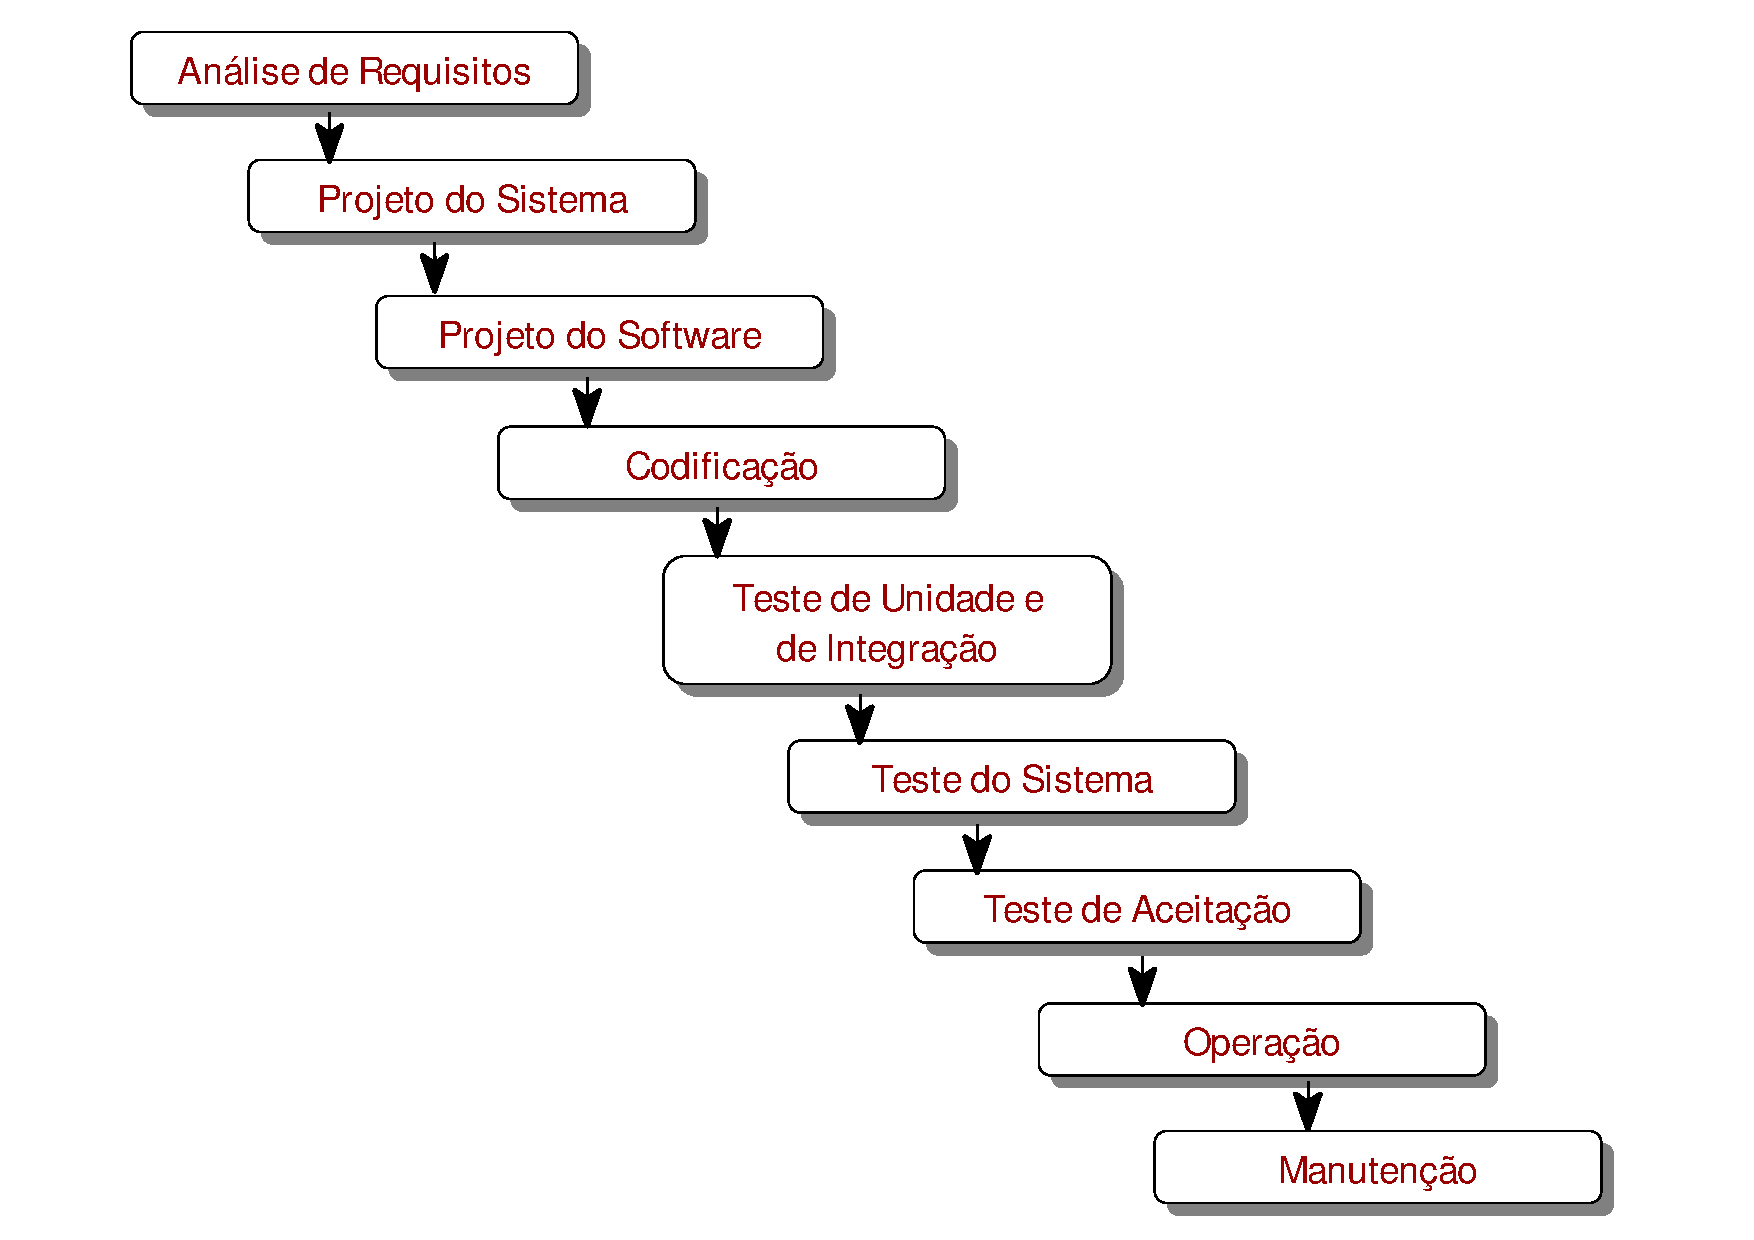
\includegraphics [width=0.75\textwidth]{cascata.pdf}
 \caption{Modelo cascata} \label{casc}
\end{figure}

Poucos anos depois, \cite{bas75}
propuseram o modelo evolucion�rio, em que o principal objetivo era
reduzir o tempo de entrega do produto em rela��o ao modelo
cascata, valorizando o desenvolvimento incremental, os ciclos
menores de desenvolvimento e a disponibiliza��o frequente de
pequenas partes do software ao cliente, ao inv�s de uma
entrega apenas ao final do desenvolvimento, como ocorria nos modelos que
o antecederam. Em 1988, sob a perspectiva dos modelos
evolucion�rios, \cite{boe88} apresentou o modelo espiral
para desenvolvimento de software, que possui, como uma de suas principais caracter�sticas, a identifica��o, an�lise e resolu��o de riscos. O modelo sugere a execu��o de diversos ciclos constitu�dos pela identifica��o de objetivos, an�lise de riscos, desenvolvimento do software e avalia��o. Uma esquematiza��o do modelo espiral � apresentada na Figura \ref{espiral}. 

\begin{figure}[!ht]
\centering
 \bfseries
   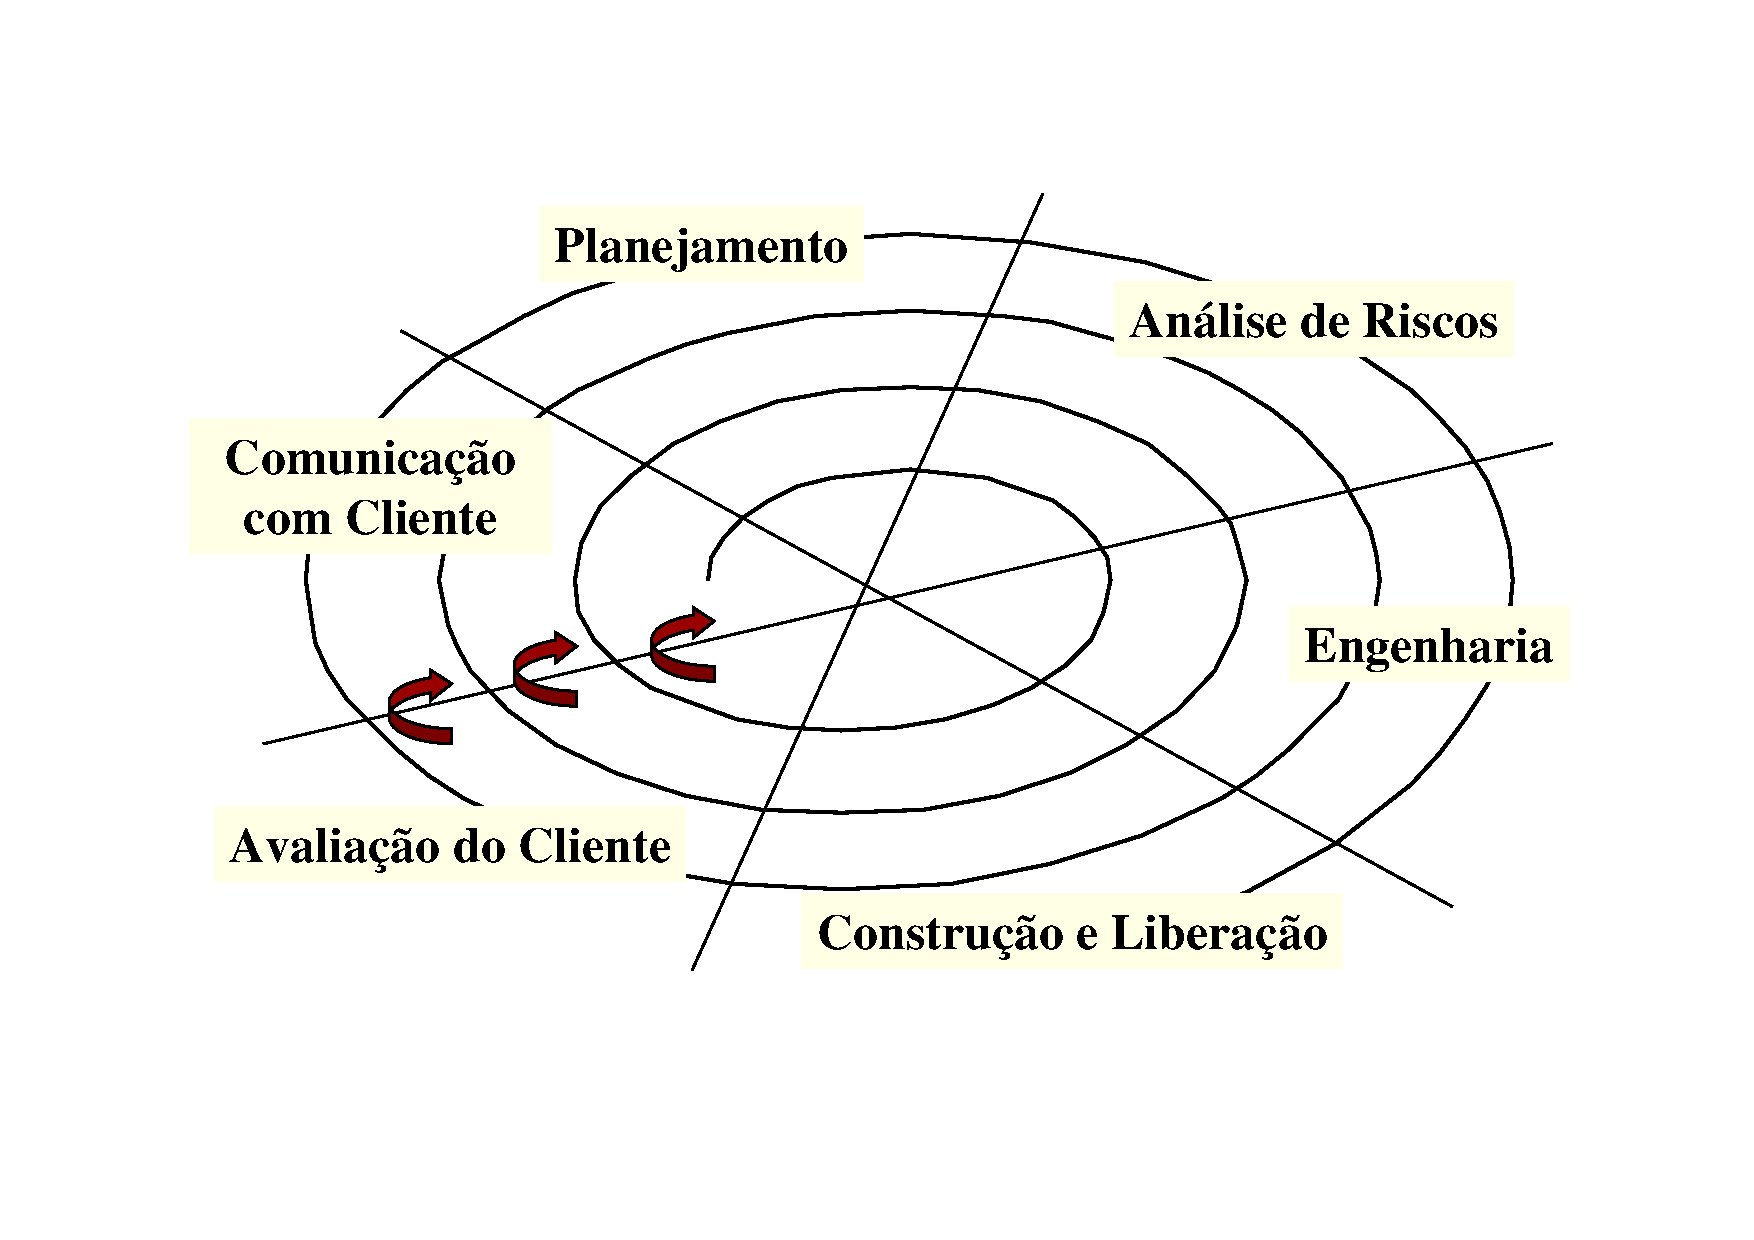
\includegraphics [width=0.75\textwidth]{espiral.pdf}
 \caption{Modelo espiral} 
 \label{espiral}
\end{figure}

Conforme indicado por \cite{mad91}, entre os principais benef�cios obtidos com a proposta dos modelos citados est�  a apresenta��o das atividades globais envolvidas na produ��o de software. Uma limita��o, no entanto, � que n�o foram apresentados detalhes importantes que s�o cruciais para o desenvolvimento de projetos de software, por exemplo, artefatos de entrada e sa�da de cada atividade e os pap�is que as pessoas envolvidas com o desenvolvimento dos projetos precisam desempenhar para que as atividades possam ser cumpridas. Assim como \cite{tyr00} (citado na se��o anterior), Madhavji destacou a import�ncia em fornecer {\it guidelines} que auxiliem a execu��o dos processos de software.

Ainda na d�cada de 1980 come�aram a ocorrer eventos para discuss�o
sobre pesquisas em processos de software, por exemplo, {\it The
Software Process Workshop}. Nesse per�odo, a
modelagem de processos de software come�ou a ser discutida e
algumas linguagens come�aram a ser propostas considerando
diferentes t�cnicas e paradigmas como base, por exemplo, Redes de
Petri e Orienta��o a Objetos \citep{kel88,hum89a}. A proposta
dessas linguagens para modelagem de processos motivou,
posteriormente, o desenvolvimento de ambientes de
Engenharia de Software centrados em processo ({\it
Process-centered Software Engineering Environments} -- PSEEs), que
oferecem um conjunto de servi�os e linguagens de modelagem de
processos para auxiliar a defini��o de processos de software \citep{gru02}.

%Conforme apresentado na Se��o X, a defini��o
%de linguagens para modelagem de processos e dos ambientes que
%fornecem aux�lio automatizado constituem uma das principais linhas
%de pesquisa na atualidade.

Ao longo dos anos, alguns pesquisadores notaram que conceitos que estavam sendo aplicados em outras �reas de conhecimento poderiam ser importantes tamb�m para o desenvolvimento de software. Por exemplo, em 1987, \cite{Broo87} expressou
claramente a import�ncia do uso de met�foras para melhorar a comunica��o entre as pessoas envolvidas com o projeto. A abordagem participativa, ou seja, o est�mulo � participa��o do usu�rio para
a defini��o de funcionalidades, avalia��o de prot�tipos e
participa��o na tomada de decis�es de projeto tamb�m foi sugerida
\citep{Gro93}. � interessante notar que abordagens mais atuais de desenvolvimento de software, por exemplo, m�todos �geis como XP ({\it eXtreme Programming}) \citep{bec99}
e FDD ({\it Feature Driven Development}) \citep{palm02} continuam a empregar tais princ�pios. Conforme observado por
\cite{Broo87},  \cite{Bry00} e \cite{Was96}, a ado��o cont�nua desses princ�pios oferece ind�cios de que eles contribuem para formar a base da disciplina de Engenharia de Software.

%Na mesma �poca em que os primeiros processos de software come�aram
%a ser propostos, diversos pesquisadores se interessaram pela
%aplica��o de determinados conceitos na Engenharia de Software que j� estavam sendo
%explorados em outras �reas de conhecimento
%Por exemplo, em 1987  em rela��o � comunica��o
%entre as pessoas envolvidas, Brooks \cite{Broo87} expressou
%claramente a import�ncia do uso da met�fora. A abordagem
%participativa, ou seja, o est�mulo � participa��o do usu�rio para
%a defini��o de funcionalidades, avalia��o de prot�tipos e
%participa��o na tomada de decis�es de projeto tamb�m foi refor�ada
%(ver ref. no artigo dos questionarios). � interessante notar que
%esses conceitos continuam sendo empregados ainda na atualidade
%(por exemplo, em m�todos �geis como XP ({\it eXtreme Programming})
%e FDD ({\it Feature Driven Development}). Conforme observado por
%Brooks \cite{Broo87}, Bryant \cite{Bry00} e Wasserman
%\cite{Was96}, isso oferece ind�cios de que esses elementos (dentre
%outros) contribuem para formar a base da disciplina de Engenharia
%de Software.

% Na d�cada de 1990, a crescente demanda em torno do desenvolvimento do software, a necessidade de diversas organiza��es em melhorar a qualidade de seus produtos e de seus processos para se tornarem competitivas e os custos elevados com manuten��o impulsionaram a realiza��o de pesquisas visando a qualidade dos sistemas de software. Assim, linguagens para modelagem de processos de software foram propostas considerando diferentes paradigmas como base, por exemplo, redes de petri e orienta��o a objetos. A proposta dessas linguagens motivou o desenvolvimento de (PSEEs), que s�o definidos como... Conforme apresentado na Se��o X, a defini��o de linguagens para modelagem de processsos e dos  ambientes que forne�em aux�lio automatizado constituem uma das principais linhas de pesquisa na atualidade.

A partir da d�cada de 1990 observou-se o surgimento de diversos modelos de aux�lio � melhoria de processos, como o modelo IDEAL \citep{GreMye97}, o modelo CMM \citep{PauWebCurChi95} (atualmente CMMI \citep{CMMI2002}), a norma ISO/IEC 12207 \citep{ISO12207} e o projeto SPICE (que culminou na norma ISO/IEC 15504 \citep{ISO15504}). %Nem todas essas propostas foram elaboradas para o contexto de desenvolvimento de software especificamente. Por�m, a import�ncia relacionada � qualidade do software produzido motivou (e ainda motiva) o desenvolvimento de diversas pesquisas relacionadas � adapta��o e extens�o dos modelos para contextos mais espec�ficos \citep{syl06,pol99}.
Ao final da d�cada de 1990, resultados de estudos cient�ficos envolvendo o processo utilizado para o desenvolvimento de projetos de software livre come�aram a ser apresentados, sendo que o trabalho de \cite{ray99} indicando os modelos Catedral e Bazar (descritos na Se��o \ref{so_livre}) foi amplamente aceito.

%Al�m disso, a defini��o e o cumprimento de atividades relacionadas ao gerenciamento de processos passaram a ser consideradas fundamentais no contexto de desenvolvimento de software \cite{hum89a}.

%Nota-se que o tema de defini��o e melhoria de processos de software continua a ser um tema atual no contexto da Engenharia de Software.  %um dos temas de interesse da comunidade cient�fica e das pessoas que praticam engenharia de software se refere, ainda hoje, � defini��o e melhoria de processos de software.
%A partir de meados da d�cada de 1990, tornou-se evidente a preocupa��o em definir m�todos �geis, que diminu�ssem a sobrecarga de atividades, tarefas e artefatos para determinados contextos; processos para o desenvolvimento de projetos desenvolvidos de forma colaborativa e por equipes geograficamente dispersas (como os processos de software livre) e processos voltados para atender ao desenvolvimento de tipos espec�ficos de software, por exemplo, software embutido ou software para sistemas de tempo real. � interessante notar que os modelos de processsos de software  discutidos na d�cada de 1970 continuam sendo empregados em pesquisas atuais. X expressa, por exemplo,  (pegar um exemplo do kiko que fala do uso do mod. cascata no dese. de softw. livre)
%Assim, nota-se que as propostas atuais s�o significativamente baseadas nos conceitos e nos modelos apresentados quando processos de software come�aram a ser investigados e praticados. Em contrapartida, isso contribui para avaliar o significado, a import�ncia e a validade desses elementos b�sicos em um espectro mais amplo, que envolve o desenvolvimento de software ao longo de diferentes �pocas, em que as diferentes disciplinas que influenciam na implementa��o das atividades de Engenharia de Software  (por exemplo, linguagens de programa��o) estavam evoluindo.

%a que deram origem atualmente a aplica��o  que a defini��o (anterior) das metodologias e a aplica��o (atual) de suas principais id�ias geram um contexto de

Outra linha de pesquisa que tem se destacado nos �ltimos anos est�
relacionada ao desenvolvimento e implanta��o de ambientes que tornem poss�vel a modelagem de processos de software e que ofere�am suporte ao
desenvolvimento de projetos distribu�dos \citep{gru02}. De acordo
com \cite{CPY00}, processos de software possuem
caracter�sticas importantes, por exemplo, s�o executados por um
per�odo longo de tempo, s�o distribu�dos e est�o sujeitos �
evolu��o constante. Conforme observado por \cite{ar02}, tais caracter�sticas t�m sido consideradas nas
pesquisas desenvolvidas nas �ltimas duas d�cadas.
No entanto, existe ainda a necessidade de que requisitos como
usabilidade e manutenibilidade dos processos tamb�m sejam
considerados nos ambientes que est�o sendo propostos.

Mais recentemente, \cite{Boe05} observou que as pesquisas e as tend�ncias em termos de Engenharia de Software est�o concentradas na proposi��o de modelos de processos de software mais adaptativos, direcionados a riscos, e que considerem os conceitos da Engenharia de Software baseada em valor, ou {\it Value-Based Software Engineering}\footnote{{\it Value-Based Software Engineering} est� relacionado ao interesse em agregar valor �s pr�ticas de Engenharia de Software j� existentes ou emergentes \citep{boe06}. Um exemplo apresentado por \cite{Gru06} � a evolu��o de processos, m�todos e ferramentas de uma abordagem individual para uma abordagem orientada a equipes.}. O autor destaca tamb�m a necessidade de pesquisas sobre a defini��o e o estabelecimento de processos colaborativos que considerem n�o somente as caracter�sticas do dom�nio de aplica��o para o qual est�o sendo propostos, mas tamb�m elementos de diversidade cultural dos membros participantes. De forma semelhante, \cite{haw05} destacam a defini��o e o estabelecimento de processos distribu�dos, que possuem, como elementos fundamentais, a comunica��o e a colabora��o entre pessoas de diferentes culturas. %De forma semelhante, Hawhorne \cite{haw05} destaca a import�ncia da defini��o de processos distribu�dos, que possuem como elementos fundamentais a comunica��o e a colabora��o entre pessoas de diferentes culturas.      %O autor destaca tamb�m que atividades colaborativas, tais como o projeto participativo, requerem suporte efetivo em termos de processos e de Engenharia de Software n�o somente em rela��o ao dom�nio de aplica��es, mas tamb�m em rela��o a diversidades culturais. Na pr�tica, muitas pesquisas precisam ser desenvolvidas para o estabelecimento de processos colaborativos globais.

Um desafio em termos de defini��o e execu��o de processos de
software se refere � necessidade de propor metodologias que sejam
�geis e, ao mesmo tempo, garantam que haja a disciplina
fundamental para o desenvolvimento de diferentes tipos de
sistemas. De acordo com \cite{boe04}, � importante propor processos de
software em que cada incremento seja direcionado � elabora��o de
planos e que sejam utilizadas abordagens �geis para auxiliar a
divulga��o e {\it marketing} do projeto, an�lise de impacto de mudan�as e
inclus�o de novas tecnologias. Isto requer novas abordagens
para gerenciamento e administra��o de projetos e para contrata��o
e aloca��o de pessoas de acordo com os aspectos din�micos do
desenvolvimento do projeto.

%A crescente exig�ncia por qualidade nos artefatos de software
%levou, nos �ltimos anos, � proposta de modelos que pudessem
%auxiliar a melhoria dos processos cumpridos. A adapta��o
%desses modelos para situa��es mais espec�ficas
%tem ocorrido com frequ�ncia.
%O modelo \cite{mpsbr}, por exemplo, � um modelo de refer�ncia para auxiliar a melhoria de processos de software em empresas brasileiras de pequeno porte. Al�m disso,  podem
%ser consideradas como tend�ncias de pesquisa em termos de
%processos de software \citep{Der04,fio01}: processos
%�geis, desenvolvimento de software livre, reutiliza��o de
%processos de software, padr�es de processo e  defini��o de
%m�tricas para promover a avalia��o e a melhoria cont�nua de
%processos.

Na Figura \ref{tempo} � apresentada uma linha de tempo resumindo
os conceitos relacionados a processos de software que foram discutidos nesta se��o. Acima da linha s�o apresentados os conceitos e as principais id�ias que emergiram em cada �poca. Os modelos resultantes s�o apresentados na parte inferior.

\begin{figure}[h]
\centering
 \bfseries
   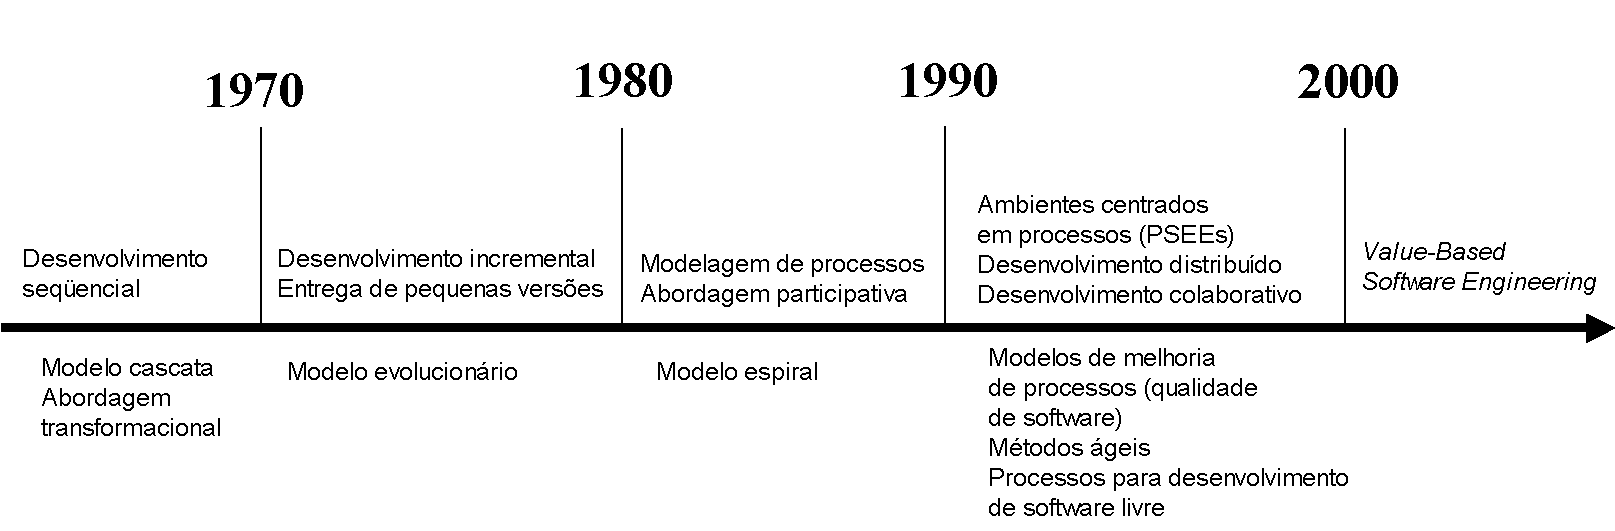
\includegraphics [width=0.95\textwidth]{linhatempo.pdf}
 \caption{Evolu��o de processos de software} \label{tempo}
\end{figure}

\section{Desenvolvimento distribu�do de projetos}

Uma importante evolu��o da Engenharia de Software (e uma tend�ncia para os pr�ximos anos, como mencionado na se��o anterior) est� associada a forma como suas atividades passaram a ser cumpridas. Inicialmente havia um enfoque individual, ou seja, cada atividade era desenvolvida por uma pessoa da equipe de desenvolvimento ou por um n�mero pequeno de pessoas, em geral, fisicamente pr�ximas. Nos �ltimos anos, com o aumento da complexidade dos projetos de software tornou-se imprescind�vel a intera��o e a colabora��o entre membros de diversas �reas de conhecimento, que muitas vezes n�o se encontram em um mesmo local de trabalho, levando � distribui��o de tarefas \citep{Arn95,haw05}.  %passou a ser valorizada a colabora��o entre as pessoas para a obten��o dos resultados esperados.

%Nos �ltimos anos, a engenharia de software tem evolu�do de uma disciplina em que as atividades eram cumpridas de uma forma individual para uma disciplina em que diferentes equipes passam colaborar no cumprimento das diversas atividades \cite{Arn95}. Conforme apresentado por Maidantchik \cite{Mai99}, com o aumento da complexidade dos projetos de software tornou-se imprescind�vel a intera��o entre membros de diversas �reas de conhecimento, que muitas vezes n�o se encontravam em um mesmo local de trabalho, levando � distribui��o de tarefas entre diversos departamentos e institui��es.

%Conforme apresentado por Maidantchik \cite{Mai99}, com o aumento da complexidade dos projetos de software tornou-se evidente a necessidade de que come�assem a ser desenvolvidos por equipes geograficamente dispersas. Um dos motivos determinantes para que os projetos passassem a ser desenvolvidos de forma distribu�da foi que o conhecimento imprescind�vel para o desenvolvimento de v�rios projetos muitas vezes n�o se encontrava em um mesmo local de trabalho, levando � distribui��o de tarefas entre divesos departamentos.

De acordo com \cite{mau98} e \cite{per97} diversos elementos
cr�ticos precisam ser considerados em processos utilizados para o
desenvolvimento distribu�do de projetos, por exemplo, comunica��o
entre os membros, acesso ao conhecimento, desenvolvimento de
atividades cooperativas e registro de experi�ncias adquiridas para
posterior reutiliza��o. 

Sob a mesma perspectiva,
pesquisadores que est�o investigando e experimentando processos de
software no desenvolvimento distribu�do de projetos indicaram as
principais atividades que os comp�em. \cite{mai99} identificou atividades que
devem ser acrescentadas � norma ISO/IEC 12207 com o objetivo de
definir um processo padr�o que possa ser utilizado por equipes
de trabalho heterog�neas, geograficamente dispersas e
culturalmente diferentes para o desenvolvimento de software.
\cite{sir05} realizaram um {\it survey} com analistas e
desenvolvedores que participaram do desenvolvimento distribu�do de
projetos com o objetivo de compreender as caracter�sticas do
desenvolvimento distribu�do, os problemas associados e poss�veis
solu��es. \cite{bat01} descreveram suas experi�ncias com o
desenvolvimento distribu�do de projetos na Motorola e indicaram as
principais caracter�sticas de um projeto distribu�do e os
problemas que geralmente s�o enfrentados pelas equipes e as
poss�veis solu��es. \cite{pri04} e e \cite{herbs05} apresentaram li��es que foram
aprendidas a partir do desenvolvimento de projetos
distribu�dos. De forma geral, os
pesquisadores destacaram a import�ncia das atividades de
gerenciamento de configura��o, comunica��o, gerenciamento e
coordena��o de projetos e defini��o e estabelecimento da
infra-estrutura. \cite{sir05}, \cite{pri04} e
\cite{herbs05} mencionaram tamb�m a import�ncia do registro de
experi�ncias e decis�es de projeto (que � um dos focos deste
trabalho) para auxiliar na divulga��o de informa��es de interesse
das equipes.

%Nesse contexto, Maidantchik \cite{Mai99} definiu um processo
%padr�o que possa ser utilizado por equipes de trabalho
%heterog�neas, geograficamente dispersas e culturalmente diferentes
%para o desenvolvimento de software, conforme apresentado na Figura
%\ref{}. Foi definida uma estrutura �nica a ser seguida pelas
%equipes distribu�das envolvidas em um projeto de software. A
%defini��o do processo teve como base a Norma ISO/IEC 12207
%\cite{ISO12207}, a qual divide as atividades do ciclo de vida do
%software em processos prim�rios, processos de apoio e processos
%organizacionais. Os processos da norma foram redefinidos e foram
%acrescentados outros processos e outras atividades para atender �s
%necessidades de equipes de trabalho dispersas.

%� poss�vel identificar na literatura um conjunto de atividades que devem ser consideradas
%em um processo para o desenvolvimento de projetos distribu�dos. Conforme apresentado
%no Quadro \ref{comp} nota-se que h� muitas semelhan�as entre as propostas em rela��o �s atividades sugeridas. Com esses resultados, como apresentado na Se��o X,  adotou-se neste trabalho o processo apresentado por Maidantchik para auxiliar a defini��o do processo proposto para o desenvolvimento de projetos de pesquisa (que possui como uma de suas principais caracter�sticas o fato de ser realizado por equipes geograficamente dispersas). O trabalho de Maidantchik foi escolhido, principalmente, devido ao fato de ter sido apresentado no formato de um processo (enquanto os outros trabalhos apresentavam basicamente pr�ticas para o desenvolvimento de projetos distribu�dos) e por haver utilizado como base a mesma estrutura (Norma ISO/IEC 12207) utilizada neste trabalho (isso facilitou a identifica��o das atividades da norma que precisariam ser alteradas para a defini��o do processo para o desenvolvimento de projetos de pesquisa considerando-se o fator de desenvolvimento distribu�do). %, ou seja, foi simples observar a correla��o entre atividades da norma e atividades do processo para o desenvolvimento de projetos distribu�dos).

%N�o foram encontradas atualiza��es do trabalho desenvolvido por Maidantchik \cite{Mai99} ap�s a proposi��o das emendas 1 e 2 da Norma ISO/IEC 12207. No entanto, ao comparar as atividades propostas por esse processo com as atividades propostas mais recentemente por outros autores para o desenvolvimento de projetos distribu�dos (ver refs. no icse 2006 - global software development), nota-se que h� muitas semelhan�as entre as propstas. No Quadro \ref{comp} � realizada uma compara��o entre as atividades propostas para o desenvolvimento de projetos distribu�dos. Com esses resultados, como apresentado na Se��o X,  adotou-se neste trabalho o processo apresentado por Maidantchik para auxiliar a defini��o do processo proposto para o desenvolvimento de projetos de pesquisa (que possui como uma de suas principais caracter�sticas o fato de ser realizado por equipes geograficamente dispersas). O trabalho de Maidantchik foi escolhido, principalmente, devido ao fato de ter sido apresentado no formato de um processo (enquanto os outros trabalhos apresentavam basicamente pr�ticas para o desenvolvimento de projetos distribu�dos) e por haver utilizado como base a mesma estrutura (Norma ISO/IEC 12207) utilizada neste trabalho (isso facilitou a identifica��o das atividades da norma original que precisariam ser alteradas para a defini��o do processo para o desenvolvimento de projetos de pesquisa, ou seja, foi simples observar a correla��o entre atividades da norma e atividades do processo para o desenvolvimento de projetos distribu�dos).

%\begin{table}[h]
%\begin{center}
%\caption{Compara��o entre propostas para o desenvolvimento de projetos distribu�dos em rela��o a atividades }\label{comp}
%\begin{tabular}{|p{3cm}|p{1.8cm}|p{1.8cm}|p{1.8cm}|p{1.8cm}|p{1.8cm}|p{1.8cm}|}
%\hline
% & \small Maidantchik \cite{Mai99} & \small Herbsleb et al \cite{herbs05} & \small Sirvio e Tihinen \cite{sir05} & \small Prikladnicki \cite{pri04} & \small Battin et al \cite{bat01} & \small  \\
%\hline \small Defini��o & \small X & \small X & \small X & \small X & \small X &\\
%\hline \small Planejamento & X & X & X & X & X &\\
%\hline \small Desenvolvimento & X & X & X & X & X &\\
%\hline \small Opera��o & X & X & X & X & X &\\
%\hline Manuten��o & X & X & X & X & X &\\
%\hline Documenta��o & X & X & X & X & X &\\
%\hline Publica��o de resultados & X & & & & &\\
%\hline Ger�ncia de configura��o & X & X & X & X & X &\\
%\hline Controle da qualidade & X & X & & & &\\
%\hline Verifica��o & X & & & & &\\
%\hline Valida��o & X & & & X & & \\
%\hline Revis�es & X & X & & & &\\
%\hline Resolu��o de Problemas & X & X & & & X &\\
%\hline Capacita��o & X & & & & &\\
%\hline Ger�ncia & X & X & X & X & &\\
%\hline Controle de Artefatos & X & & & & &\\
%\hline Melhoria & X & X & & X & & \\
%\hline Comunica��o & X & X & X & X & X &\\
%\hline Coordena��o & X & & & & X & \\
%\hline Infra-estrutura & X & X & X & X & X &\\
%\hline Treinamento & X & X & X & X & &\\
%\hline Rastreio de informa��es & & X & & X & &\\
%\hline Aux�lio � pr�tica & & X & X & & &\\
%\hline Gerenciamento de conhecimento & & & X & X & &\\
%\hline Registro de experi�ncias e decis�es de projeto  & & X & X & X & &\\
%\hline Transfer�ncia de conhecimento & & & X & & &\\
%\hline Recrutamento & & & & X & &\\
%\hline
%\end{tabular}
%\end{center}
%\end{table}

Nota-se que h� uma demanda n�o somente em rela��o a processos para
o desenvolvimento distribu�do de projetos, mas tamb�m em rela��o
a ambientes e ferramentas que possam apoiar o cumprimento desses
processos. A plataforma GENESIS ({\it GEneralised eNvironment for procEsS
management in cooperatIve Software engineering}) \citep{aver04},
por exemplo, est� sendo desenvolvida como um projeto de
pesquisa que tem como objetivo projetar e desenvolver um sistema
para apoiar processos de Engenharia de Software em um ambiente
distribu�do. Dentre outras funcionalidades, o sistema oferece recursos para apoio 
� coopera��o, � coordena��o dos processos, � modelagem e
decomposi��o dos processos em sub-processos (de forma que possam
ser executados por diferentes equipes) e ao gerenciamento de
recursos, de artefatos e de dados.

De forma semelhante, foi
proposto por \cite{kot99} um sistema para
gerenciamento de {\it workflow}, denominado MILOS, que utiliza
recursos da internet para apoiar a coordena��o din�mica de
equipes de desenvolvimento de software. Uma das principais
caracter�sticas do sistema � o suporte ao desenvolvimento de
projetos de software �geis e distribu�dos \citep{bow02}.

\cite{kam98}, \cite{kry03} e \cite{gia01} tamb�m propuseram ambientes para apoiar o desenvolvimento de projetos distribu�dos. De forma geral, as principais funcionalidades implementadas est�o relacionadas � defini��o e especifica��o de artefatos, atividades e recursos do processo, coordena��o do processo cumprido pelas equipes, gerenciamento de {\it workflow} (cria��o, execu��o e monitoramento do workflow) e apoio � comunica��o.

%Em termos de processos de software para o desenvolvimento distribu�do de projetos de pesquisa foi encontrado na literatura o trabalho de \cite{Oli05} (descrito na Se��o \ref{xr}) em que foi proposta uma adapta��o da metodologia XP para o contexto de pesquisas desenvolvidas de forma distribu�da. De forma geral, os autores apresentam as pr�ticas de XP sob uma perspectiva de desenvolvimento de pesquisa e de um ambiente em que h� equipes geograficamente dispersas. As atividades discutidas nesta se��o para o cumprimento de processos distribu�dos foram parcialmente contempladas na proposta. Foram valorizadas, especialmente, a comunica��o entre os membros das equipes e o compartilhamento de conhecimento. No entanto, outras pr�ticas fundamentais, por exemplo, gerenciamento de configura��es, n�o foram inclu�das.


%POSSO ENFATIZAR ACRESCENTANDO:

%Foram apresentadas tamb�m experi�ncias com a execu��o de processos distribu�dos em ambiente de desenvolvimento de pesquisa (colocar refs. sobre XP, collaboraratories, e-Science). As li��es aprendidas destacadas pelos autores s�o:


%Este estudo foi importante no sentido de auxiliar o entendimento
%do estado da pr�tica em termos de suporte automatizado para o
%cumprimento de processos distribu�dos e, consequentemente, na
%identifica��o de ferramentas que pudessem ser sugeridas como parte
%da instancia��o do processo, conforme apresentado na Se��o X.


 %� poss�vel tamb�m coletar m�tricas durante o cumprimento do processo com o objetivo de melhorar o desenvolvimento do projeto. Outro fator positivo � o fato de ter sido experimentada em ambiente acad�mico e industrial e estar em constante evolu��o. No entanto, o fato de os pr�prios desenvolvedores terem participado ativamente das avalia��es pode ser considerada uma amea�a � validade da avalia��o realizada. Al�m disso, poucos dados quantitativos foram apresentados como resultado das avalia��es.

%Diversas li��es aprendidas foram apresentadas por pesquisadores envolvidos no projeto e desenvolvimento de ambientes e ferramentas que podem ser utilizadas em desenvolvimento de projetos distribu�dos \cite{sir05,ger04} e por participantes do desenvolvimento de projetos distribu�dos \cite{ger04,jacch93} foram importantes no contexto deste trabalho no sentido de auxiliar na defini��o dos elementos fundamentais que deveriam ser considerados na elabora��o do processo proposto neste trabalho. Um resumo dessas li��es aprendidas � apresentado a seguir:


\section{Desenvolvimento colaborativo de projetos}

Conforme apresentado na se��o anterior, um dos principais fatores que motivaram a mudan�a de paradigma em rela��o a forma de desenvolvimento de projetos de software (de uma abordagem individual para uma abordagem voltada para equipes) foi o aumento da complexidade desses projetos e a necessidade de colabora��o entre pessoas de diferentes �reas de conhecimento. O advento da internet e os avan�os tecnol�gicos em termos de redes de comunica��o foram fatores fundamentais que possibilitaram que a mudan�a ocorresse.   %ofereceram sub}{} , os projetos come�aram a ser desenvolvidos de forma distribu�da, de forma que o conhecimento de

%Nesse contexto, a colabora��o entre membros que participam do desenvolvimento dos projetos tamb�m passou a ser valorizada. Tornou-se poss�vel que pessoas localizadas em regi�es geogr�ficas distantes pudessem colaborar, por exemplo, no desenvolvimento de um mesmo modelo ou de uma parte do c�digo. Conforme apresentado por \cite{uwa06} \cite{Bol04}, \cite{numpra03}, a colabora��o tem sido observada como um importante fator que possibilita o desenvolvimento de projetos de pesquisa e contribui para a obten��o de qualidade nos estudos cient�ficos. 

Uma abordagem de desenvolvimento colaborativa se refere ao envolvimento de diversos grupos de pessoas trabalhando conjuntamente no desenvolvimento de um projeto, para benef�cio de todos os participantes \citep{uwa06}. O TSP ({\it Team Software Process}) foi proposto por \cite{hum99} como uma evolu��o do PSP, com a finalidade de servir a grupos de pessoas que tenham por objetivo desenvolver software de qualidade. De forma geral, o PSP foi projetado para auxiliar estudantes e engenheiros de software a organizar e planejar seus trabalhos, medir seus desempenhos, gerenciar a qualidade de software e analisar e melhorar seus processos. No TSP s�o apresentados {\it guidelines}, atividades, ferramentas, m�todos e t�cnicas para desenvolver software por equipes. O TSP � baseado em um modelo incremental, sendo que as atividades que comp�em cada ciclo de desenvolvimento s�o cumpridas de forma sequencial. % se precisar de figura: Conforme apresentado na Figura \ref{tsp} (figura 1 do artigo teams need a process) + as descri��es das fases na tabela do artigo.

Os participantes da equipe de desenvolvimento s�o organizados de
forma que cada desenvolvedor desempenhe um ou dois pap�is
gerenciais bem definidos. Os pap�is suportados pelo processo s�o
os de gerente de desenvolvimento, de planejamento, de qualidade,
de processo, de suporte e de l�der da equipe. O planejamento e o
controle rigoroso de tamanhos, esfor�os, prazos e defeitos
apresentados no PSP tamb�m foram considerados no TSP. Os
principais processos enfatizados no TSP s�o gest�o de requisitos,
planejamento e controle de projetos, garantia da qualidade e
gerenciamento de configura��o.

De acordo com \cite{hil00}, o TSP oferece um excelente {\it
framework} para auxiliar estudantes no aprendizado da pr�tica
profissional de Engenharia de Software e, sobretudo, como
trabalhar em uma equipe para o desenvolvimento de software. Como
desvantagem, o autor menciona que o cumprimento do processo �
bastante oneroso em termos de tempo gasto para cumprir as
atividades propostas e coletar os dados sugeridos. Al�m disso,
como indicado por \cite{Pressman05}, a aplica��o do PSP e do TSP
exige treinamento extensivo e muita disciplina das pessoas
envolvidas no desenvolvimento dos projetos. \cite{PaulaFilho01}
observou tamb�m, a partir de experi�ncias pr�ticas, que a
aplica��o dos processos � bem sucedida quando os membros das
equipes possuem excelente conhecimento em Engenharia de Software e
possuem motiva��o para empregar processos de software em n�vel
avan�ado.

Nota-se, portanto, que o requisito de que as pessoas envolvidas
possuam conhecimentos avan�ados em Engenharia de Software
desfavorece a aplica��o direta do TSP no contexto de
desenvolvimento de projetos de pesquisa. � comum que os estudantes
e pesquisadores n�o possuam experi�ncia na realiza��o das diversas
atividades, que envolve, por exemplo, controle de qualidade e
gerenciamento do projeto. No processo proposto neste trabalho, tendo em vista o aux�lio � execu��o e evolu��o de projetos de pesquisa em software,  considera-se que os
participantes podem ser \textit{aprendizes} e que a participa��o em um
projeto de pesquisa pode ser, inclusive, uma de suas primeiras
experi�ncias pr�ticas.

%Pesquisadores que est�o investigando ou experimentando processos em desenvolvimento de projetos colaborativos identificaram algumas atividades que consideraram muito importantes projetos, conforme indicado a seguir:

%Uma breve descri��o de trabalhos relacionados a processos colaborativos de software � apresentada a seguir. Foram destacadas, em especial, as atividades que comp�em os processos colaborativos. Outros trabalhos relacionados a processos colaborativos de software s�o indicados a seguir:

Pesquisadores que est�o investigando e experimentando processos de software no desenvolvimento colaborativo de projetos indicaram as principais atividades que devem ser consideradas. \cite{paa04} realizaram entrevistas com participantes de oito projetos desenvolvidos de forma colaborativa em que foi solicitado que eles indicassem as atividades que consideraram mais importantes para o sucesso dos projetos; \cite{Aug02} discutiram as pr�ticas de desenvolvimento de software colaborativo que eles consideraram mais importantes de acordo com suas experi�ncias no desenvolvimento de projetos colaborativos; \cite{eber01} apresentaram, considerando suas experi�ncias em uma empresa de telecomunica��es,  pr�ticas que julgam relevantes e que consideram que devam ser cumpridas com efetividade para que o desenvolvimento de projetos colaborativos seja bem sucedido; \cite{Pin02} e \cite{ara07} propuseram ferramentas que auxiliam o desenvolvimento colaborativo de projetos. De forma geral, os autores destacaram a pr�tica de defini��o de pap�is e do apoio � comunica��o entre os membros das equipes. Notou-se, ainda, que os autores mencionaram usando diferentes nomenclaturas, a import�ncia da {\it percep��o} do trabalho desenvolvido pelos membros dos grupos. � interessante notar que as pr�ticas indicadas pelos autores s�o semelhantes e est�o bastante relacionados �s pr�ticas para o desenvolvimento distribu�do de projetos. De fato, conforme indicado por \cite{coo04}, para que a engenharia de software colaborativa possa ser cumprida de fato, �reas de pesquisa como visualiza��o de software, intera��o usu�rio-computador e desenvolvimento distribu�do devem
contribuir efetivamente, ou seja, a interse��o entre essas �reas forma a base do desenvolvimento colaborativo.

%Durante o desenvolvimento deste trabalho n�o foram encontrados processos espec�ficos que tratassem o desenvolvimento colaborativo de projetos de pesquisa. Foram encontrados somente relatos de experi�ncias envolvendo desenvolvimento de pesquisa em um ambiente de colabora��o, no qual n�o foi evidenciado um processo \citep{rog98}. De forma geral, os autores destacaram a comunica��o como um das principais atividades que contribu�ram para a obten��o dos resultados esperados.

Diversos ambientes virtuais colaborativos foram propostos nos �ltimos anos, dentre eles os sistemas DIVE \citep{hag96}, Manufaktur \citep{mon00} e CARAMBA \citep{dus04}. As funcionalidades implementadas s�o bastante semelhantes e se referem basicamente ao compartilhamento da �rea de trabalho, gerenciamento do projeto, gerenciamento do conhecimento adquirido, gerenciamento de documenta��o e comunica��o.


%O requisito de que as pessoas possuam conhecimentos avan�ados em engenharia de software para que as pr�ticas do TSP possam ser cumpridas foi um fator que desmotivou a utiliza��o direta do TSP (no sentido de indicar pr�ticas para o cumprimento de processos colaborativos) de forma que pudesse servir como base para a defini��o do processo proposto neste trabalho. � comum que

%(ver se no livro fala que � pra nivel avan�ado)

%Conforme apresentado no Quadro X, foram identificadas pr�ticas que s�o importantes para o cumprimento de processos colaborativos a partir de estudos publicados na literatura com o objetivo de inclui-las na defini��o do processo apresentado neste trabalho. De forma geral, essas pr�ticas se referem a representa��o do processo e de pontos de colabora��o, ao gerenciamento do projeto, ao estabelecimento de pap�is a membros das equipes, � comunica��o sobre o progresso do projeto e ao uso de ferramentas que favore�am o desenvolvimento colaborativo (por exemplo, editores, ferramentas de comunica��o) \cite{paa04,Aug02,Pin02,Arn95}.

%Foi realizada uma compara��o entre al Dessa forma, optou-se por analisar outros trabalhos apresentados na literatura sobre pr�ticas para processos colaborativos e consider�-las na defini��o do processo proposto. O estudo realizado por Paasivaara e Lassenius \cite{paa04}, por exemplo, teve por objetivo coletar pr�ticas de colabora��o que realmente s�o usadas no desenvolvimento de projetos de sofware inter-organizacional e que s�o percebidas como �teis. De forma geral, essas pr�ticas se referem a sincroniza��o dos principais {\it milestones} dos processos cumpridos pelas organiza��es, entregas frequentes, estabelecimento de pap�is a membros das equipes e identifica��o de quais pap�is precisam se comunicar, identifica��o de pr�ticas de resolu��o de problemas, comunica��o sobre o progresso do projeto e incentivo ao relacionamento entre os membros das equipes. Al�m disso, os autores apresentaram solu��es simples para resolver problemas comuns do desenvolvimento de projetos colaborativos, por exemplo, ter uma pessoa dedicada para auxiliar na resolu��o de problemas e esclarecimento de d�vidas (esta solu��o � semelhante ao item {\it Aux�lio � pr�tica} indicado no Quadro \ref{comp}) e criar listas de email para os projetos.

%De forma semelhante, Augustin et al \cite{Aug02}, Pinheiro et al \cite{Pin02} e Arnold \cite{Arn95} indicaram pr�ticas importantes para o desenvolvimento de projetos colaborativos e que certamente devem ser consideradas na defini��o de processos para o desenvolvimento de projetos colaborativos e na sele��o de ferramentas. No Quadro \ref{col} � apresentada uma compara��o entre as pr�ticas apresentadas pelos autores.
%Essas pr�ticas, se referem a defini��o de pap�is, adapta��o dos diferentes processos cumpridos pelas equipes para um ambiente de colabora��o, representa��o do processo e dos pontos de colabora��o que devem ser compartilhados entre os membros do grupo, integra��o de c�digo e de outros artefatos, ger�ncia de configura��o, uso de ferramentas de edi��o colaborativa, uso de ferramentas de comunica��o s�ncronas e ass�ncronas, coordena��o das atividades, registro do conhecimento comum ao grupo e percep��o do grupo em rela��o ao contexto de trabalho.
  %� poss�vel notar que h� semelhan�as entre requisitos para desenvolvimento   s�o semelhantes �queles

%\begin{table}[h]
%\begin{center}
%\caption{Compara��o entre propostas para o desenvolvimento de projetos colaborativos em rela��o a atividades }\label{comp}
%\begin{tabular}{|p{4cm}|p{2cm}|p{2cm}|p{2cm}|p{2cm}|p{2cm}|}
%\begin{tabularx}{|X|X|}
%\hline
 %& Paasivaara e Lassenius \cite{paa04} & Augustin et al \cite{Aug02} & Arnold \cite{Arn95} & Ebert and De Neve \cite{eber01}& Pinheiro et al \cite{Pin02,ara02} \\
%\hline Sincroniza��o de {\it milestones} & X &  &  & X & \\
%\hline Entregas frequentes & X & X &  & X & \\
%\hline Defini��o de pap�is & X &  & X & X & X  \\
%\hline Identifica��o da necessidade de comunica��o entre pap�is & X &  &  &  & X \\

%\hline Resolu��o de problemas & X &  &  &  & \\
%\hline Apresenta��o de informa��es sobre o progresso do projeto & X &  &  & X & \\
%\hline Incentivo ao relacionamento entre os membros & X  &  &  &  & \\
%\hline Comunica��o &  & X & X & X & \\
%\hline Captura e gerenciamento de conhecimento &  & X &  &  X & \\
%\hline Registro de decis�es de projeto &  &  &  & X & \\
%\hline Reuso de c�digo e de conhecimento &  & X &  &  & \\
%\hline Defini��o de regras e processos de desenvolvimento &  &  & X &  & \\
%\hline Cumprir boas pr�ticas de modelos de qualidade de software &  &  &  & X & X \\
%\hline Conhecimento geral sobre as atividades e o grupo (percep��o) &  &  &  & X & X \\
%\hline
%\end{tabular}
%\end{center}
%\end{table}

\section{Processo de software livre} \label{so_livre}

Software livre pode ser definido como qualquer software cuja licen�a garanta aos usu�rios liberdade para usar, copiar, distribuir, estudar, modificar e melhorar o software \citep{free06,op06}. Esta defini��o, embora seja adotada por entidades importantes que lidam com o desenvolvimento de software livre, enfatiza o produto final gerado. � importante destacar tamb�m determinadas caracter�sticas com as quais o desenvolvimento de software livre est� associado \citep{Ray01}:

\begin{enumerate}

\item Desenvolvimento descentralizado via internet: quando h� mais de uma pessoa envolvida, o desenvolvimento � realizado de forma colaborativa, usando a internet como meio de comunica��o (sites {\it web} e FTP, reposit�rios de vers�es e correio eletr�nico).

\item Participa��o dos usu�rios:  � comum a forma��o de um grupo de usu�rios finais que se comunicam com alguma regularidade com os desenvolvedores e entre si, comunicando problemas e trocando experi�ncias sobre o uso do software.

\item Interesse pessoal do autor: geralmente o autor � um usu�rio do software e, portanto, tem motiva��o pessoal na sua cria��o e manuten��o.

\item Desenvolvimento distribu�do e ferramentas de comunica��o: s�o usadas diversas ferramentas
e servi�os para suportar a comunica��o entre os indiv�duos, que geralmente encontram-se geograficamente distribu�dos.

\end{enumerate}

Os modelos utilizados para desenvolvimento de software livre apresentam caracter�sticas diferentes em rela��o aos modelos tradicionais de Engenharia de Software \citep{sca06}. Em projetos de software livre, os artefatos produzidos s�o disponibilizados em reposit�rios de controle de vers�es e n�o h� um regime formal para o gerenciamento dos projetos, dos custos e dos prazos. Em um dos principais trabalhos realizados nesse sentido, \cite{ray99} identificou dois modelos distintos para software livre: (1) o modelo Catedral, em que os projetos
de software livre s�o desenvolvidos por grupos fechados, em longos ciclos de desenvolvimento (e consequentemente com muita demora para a libera��o das vers�es) e com pequena abertura � participa��o externa e (2) o modelo Bazar, que descreve projetos desenvolvidos de forma mais transparente, abertos � participa��o de desenvolvedores que tenham interesse, com tempo de desenvolvimento curto e alta qualidade.

Algumas pesquisas t�m sido realizadas com o objetivo de entender e caracterizar o processo de desenvolvimento de software livre \citep{Fel00,rei99}. De acordo com \cite{Reis03}, podem ser observadas muitas
varia��es nos processos utilizados para o desenvolvimento dos projetos e, portanto, devem ser evitadas generaliza��es.

Apesar de n�o haver um processo estabelecido, que sirva como refer�ncia para os desenvolvedores de software livre (a modelagem do processo de software livre e a simula��o sobre como ele opera ainda � um desafio de pesquisa), pode-se notar que algumas atividades principais geralmente s�o cumpridas.
Assim, de acordo com \cite{Reis03} e \cite{zha03}:

\begin{itemize}

\item h� pouca �nfase nas fases de especifica��o de requisitos e de projeto e muitos esfor�os s�o direcionados � fase de codifica��o;
\item as atividades de gerenciamento de configura��o de software e rastreamento de {\it bugs} s�o cumpridas em grande parte dos projetos;
\item os testes s�o realizados intensivamente pelos usu�rios, que colaboram indicando {\it bugs} e sugerindo melhorias;
\item a documenta��o enfatiza principalmente as funcionalidades do software. S�o cumpridas atividades de documenta��o simples, como elabora��o de listas contendo as tarefas pendentes ({\it TODO lists}) e elabora��o de um guia de instala��o;
\item revis�es de c�digo s�o realizadas com frequ�ncia.

\end{itemize}

\subsubsection{Ferramentas}

Nota-se que ferramentas de controle de vers�es, listas de correio eletr�nico e outras ferramentas de comunica��o s�o amplamente utilizadas na comunidade de software livre. Uma parcela menor, por�m significativa, dos participantes utiliza sistemas de acompanhamento de
altera��es. Assim, observando-se as ferramentas mais comumente utilizadas, � poss�vel identificar os processos
mais valorizados. Pode-se observar que o cumprimento de atividades que oferecem suporte � comunica��o entre os membros que participam dos projetos e atividades relativas ao gerenciamento de configura��o � um
dos fatores mais importantes para o sucesso dos projetos. 

Para coordenar o trabalho que realizam, os membros da comunidade
de um projeto utilizam a internet e ferramentas simples
amplamente dispon�veis: correio eletr�nico, p�ginas {\it web}, listas de
discuss�o e ferramentas de desenvolvimento de
software. Em geral, os membros dos projetos tendem a usar estes
ve�culos para comunicar experi�ncias, problemas e solicita��es. O
uso intensivo dessas ferramentas ap�ia o desenvolvimento de
projetos distribu�dos, como
ocorre no contexto da maioria dos projetos de software livre \citep{Reis03}.

� poss�vel observar que existem caracter�sticas em comum em rela��o ao desenvolvimento de software livre e desenvolvimento de projetos de pesquisa. De acordo com  \cite{alp05}, a experi�ncia obtida com o desenvolvimento de projetos de software livre deve ser observada por pesquisadores interessados em desenvolver pesquisa colaborativa.  Conforme apresentado por \cite{bez99} e \cite{Amb04} h� muitas similaridades entre os processos de software livre e os processos acad�micos. Por exemplo, o desenvolvimento distribu�do e colaborativo pode ser considerado uma caracter�stica importante em ambas as abordagens. Os
autores sugerem que dificuldades comuns no desenvolvimento
de software em ambiente de pesquisa, como a comunica��o e a
coordena��o de projetos, sejam resolvidas utilizando-se pr�ticas e
ferramentas amplamente utilizadas na comunidade de software livre, como ferramentas de gerenciamento de mudan�as e de vers�es. De forma similar, eles observam que atividades comumente cumpridas no
desenvolvimento de projetos de pesquisa podem ser adotadas por
desenvolvedores de software livre com o objetivo de solucionar problemas que t�m sido percebidos por eles.
Por exemplo, na comunidade de software livre h� grande preocupa��o em rela��o ao n�vel de conhecimento entre especialistas e novatos. Em ambiente acad�mico, h� disponibilidade e interesse em treinar desenvolvedores novatos, mas isso nem sempre ocorre no desenvolvimento de software livre. Ambati e Kishore sugeriram, portanto, adotar a id�ia de ``comunidade de assistentes de ensino'' no contexto de software livre, da forma como ocorre em ambiente acad�mico.

 %Os autores destacam que � importante fazer uma analogia entre a forma de trabalho da comunidade cient�fica e da comunidade de software livre e identificar as experi�ncias bem sucedidas que possam ser adotadas por ambas.


%Massey \cite{mas02} discutiu as diferen�as em rela��o ao projeto de engenharia de requisitos em projetos convencionais e o processo em projetos de software livre. O autor observou a aus�ncia de um processo formal de requisitos e foram apresentadas algumas hip�teses para explicar a aus�ncia do processo de requisitos, destancando-se o fato de que os requisitos podem originar diretamente dos pr�prios desenvolvedores.


%ver artigo do sbqs 2006
%ver artigo do Maurer, se��o 2.1

\section{M�todos �geis}

Em 2001, um grupo de profissionais experientes em desenvolvimento de software se reuniu com o objetivo de discutir alternativas para as abordagens tradicionais de desenvolvimento de software, que s�o fortemente baseadas em documenta��o. Como resultado dessa reuni�o, foi criado o Manifesto para o Desenvolvimento �gil de Software (ou Manifesto �gil) \citep{manif01}, para o qual foram defendidos os seguintes valores:

%Em 2001, um grupo de representantes de diversos m�todos para desenvolvimento de software, ou seja, do XP (eXtreme
%Programming) (Beck, 2000), SCRUM (K.Schwaber e Beedle, 2002), DSDM (Dynamic System Development
%Method) (Stapleton, 1997), desenvolvimento de software adaptativo, Crystal, FDD
%(Feature-Driven Development) (Coad, 1999), e programa��o pragm�tica (Hunt e Thomas, 1999), se reuniu com o objetivo de discutir abordagens alternativas aos m�todos tradicionais para o desenvolvimento de software. De forma geral, o grupo concordava em rela��o a um conjunto de princ�pios deveria ser respeitado para que um projeto seja bem sucedido. Como resultado dessa reuni�o, foi criado o Manifesto para o Desenvolvimento �gil de Software, (ou Manifesto �gil), e o termo desenvolvimento �gil passou a descrever abordagens de desenvolvimento de software que seguissem tais princ�pios, que s�o:

\begin{itemize}

\item Pessoas e intera��es s�o mais importantes que processos e ferramentas;

\item Software funcional � mais importante que documenta��o detalhada;

\item Colabora��o do cliente � mais importante que negocia��o e

\item Resposta a mudan�as � mais importante que cumprimento de um plano.

\end{itemize}

Al�m disso, foram identificados doze princ�pios que regem a metodologia �gil de desenvolvimento de software: (1) entregar vers�es continuamente e o mais cedo poss�vel; (2) permitir mudan�as de requisitos
em qualquer fase do desenvolvimento; (3) entregar vers�es do software, que funcionam
adequadamente, em curtos per�odos de tempo (de algumas semanas a alguns meses); (4) desenvolver o projeto com a participa��o de clientes; (5) fornecer infra-estrutura necess�ria para que os clientes se sintam motivados e desempenhem o trabalho esperado; (6) incentivar a comunica��o face a
face; (7) alcan�ar a medida prim�ria de progresso, que � o software operacional; (8) manter
harmonia entre clientes, desenvolvedores e usu�rios; (9) preocupar-se com a qualidade t�cnica
e com a execu��o de bons projetos; (10) projetar com simplicidade; (11) permitir que equipes da
pr�pria organiza��o participem da defini��o da arquitetura, requisitos e projeto do sistema
e (12) permitir que as equipes, em intervalos regulares, expressem como podem se tornar mais
eficientes.

M�todos que considerassem esses princ�pios foram denominados m�todos �geis. De acordo com \cite{hig01}, a novidade dos m�todos �geis n�o s�o as pr�ticas propostas, mas sim o reconhecimento de que {\it pessoas} s�o os principais elementos para o sucesso dos projetos. %Destaca-se tamb�m que h� um intenso foco em efetividade e adaptabilidade.
Os autores destacam tamb�m que, de forma geral, m�todos �geis s�o projetados com o objetivo de (1) auxiliar a produ��o das primeiras vers�es do software em semanas, possibilitando a obten��o de {\it feedback} r�pido, (2) produzir solu��es simples, (3) auxiliar a melhoria de qualidade continuamente, tornando a pr�xima itera��o menos custosa e (4) promover a execu��o de testes constantemente, de forma que defeitos sejam identificados o quanto antes, a custos mais baixos.

%Metodologias �geis para desenvolvimento de software come�aram a ser investigadas, principalmente, com o objetivo de auxiliar a produ��o de software de alta qualidade, no prazo estipulado e considerando que pedidos de mudan�a provavelmente ocorrer�o com frequ�ncia.

\cite{wil03} indicaram as circunst�ncias nas quais m�todos �geis devem ser usados: o sistema a ser desenvolvido n�o � de miss�o cr�tica, os requisitos mudam com frequ�ncia, a equipe de desenvolvimento � pequena e situada na mesma localidade e clientes, usu�rios e especialistas no dom�nio do problema est�o dispostos a colaborar no desenvolvimento. Conforme apresentado por \cite{kir01} e por \cite{yap05} foi observada, mais recentemente, a possibilidade de que m�todos �geis sejam utilizados tamb�m por equipes distribu�das.

� poss�vel observar semelhan�as entre as caracter�sticas do ambiente de desenvolvimento de projetos de pesquisa para o qual o processo apresentado nesta tese est� sendo proposto e as caracter�sticas do ambiente no qual m�todos �geis podem ser utilizados. Pretende-se que o processo %sirva ao desenvolvimento de sistemas de informa��o
seja utilizado por equipes pequenas e geograficamente dispersas. Outra caracter�stica em comum se refere �s mudan�as frequentes dos requisitos. Conforme apresentado por \cite{seg05} e \cite{hul05}, os requisitos de um prot�tipo resultante de um projeto de pesquisa s�o definidos gradualmente, � medida que o projeto � desenvolvido. Esses requisitos mudam com frequ�ncia, de acordo com os resultados e o progresso do projeto. %Al�m disso, pesquisadores e estudantes s�o os pr�prios clientes, desenvolvedores e especialistas no dom�nio. Eles tamb�m se beneficiam dos resultados do projeto e, portanto, possuem interesse em colaborar mutuamente em prol da evolu��o de suas pesquisas.

%Deve-se destacar tamb�m que pessoas s�o mais importantes que processos em m�todos �geis. Em ambiente acad�mico, em que as pesquisas s�o desenvolvidas, a forma��o dos estudantes e dos pesquisadores � um dos fatores primordiais. (acrescento mais coisas aqui?)


As atividades que comp�em os m�todos �geis variam de acordo com as diferentes abordagens propostas na literatura, tais como, {\it eXtreme Programming} (XP) \citep{bec99}, SCRUM \citep{sch02} e {\it Feature Driven Development} (FDD) \citep{palm02}. Uma descri��o breve dos m�todos, baseada em \cite{abr02}, � apresentada a seguir.

\begin{description}

\item {\it eXtreme Programming} (XP): o ciclo de vida de XP consiste em cinco fases: explora��o, planejamento, itera��es para produ��o de releases, produ��o, manuten��o e finaliza��o \citep{bec99}. Na fase de explora��o, os clientes escrevem as est�rias que eles querem que sejam inclu�das na primeira {\it release}. Ao mesmo tempo, a equipe de projeto familiariza-se com as ferramentas, tecnologias e pr�ticas que ser�o usadas no projeto. S�o exploradas possibilidades de arquitetura para o sistema. Na fase de planejamento, � definida uma ordem para as est�rias e � feito um acordo sobre o conte�do da primeira {\it release}. Os programadores estimam esfor�o e prazo requeridos para cada est�ria. Na fase de itera��es, o cronograma definido na fase anterior � divido em um n�mero de itera��es. Na primeira itera��o � criada a arquitetura de todo o sistema. Os clientes decidem as est�rias que ser�o selecionadas para cada itera��o. Os testes funcionais s�o executados ao final de cada itera��o. Ao final da �ltima itera��o, o sistema est� pronto para a fase de produ��o, em que s�o realizados novos testes e � avaliado o desempenho do sistema. Depois que a primeira {\it release} � entregue ao cliente, a equipe de projeto deve manter o sistema em produ��o. Assim, na fase de manuten��o, o esfor�o � direcionado � tarefas de suporte ao cliente. A fase de finaliza��o ocorre quando o cliente n�o possui mais est�rias a serem implementadas. Este � o momento em que a documenta��o do sistema � escrita. A finaliza��o pode ocorrer tamb�m se o sistema n�o est� produzindo os resultados esperados ou torna-se muito caro.

\item SCRUM: o ciclo de vida do SCRUM consiste em tr�s fases: pr�-desenvolvimento, desenvolvimento e p�s-desenvolvimento \citep{sch02}. Na fase de pr�-desenvolvimento � definido o sistema que ser� desenvolvido e os requisitos que ser�o considerados. Os requisitos s�o priorizados e o esfor�o para o desenvolvimento � estimado. Al�m disso, � definida a equipe de projeto e as ferramentas que ser�o utilizadas, s�o identificados os recursos dispon�veis e os riscos do projeto e � elaborado um projeto de alto n�vel do sistema. A fase de desenvolvimento corresponde � parte �gil do SCRUM. Vari�veis relacionadas a tempo, qualidade, requisitos, recursos, tecnologias e ferramentas s�o controladas. Nesta fase, o sistema � desenvolvido em {\it sprints}, que s�o ciclos iterativos em que a funcionalidade � desenvolvida ou melhorada para produzir novos incrementos. Cada {\it sprint} inclui as fases tradicionais do desenvolvimento de software: requisitos, an�lise, projeto, evolu��o, testes e disponibiliza��o. Na fase p�s-desenvolvimento ocorre o fechamento da {\it release}. Nesta fase o sistema est� pronto para ser liberado, o que exige que o teste de integra��o e o teste de sistema tenham sido realizados e que a documenta��o esteja dispon�vel.

\item {\it Feature Driven Development} (FDD): o ciclo de vida do FDD consiste em cinco fases sequenciais \citep{palm02}. A primeira fase consiste no entendimento geral do sistema, ou seja, a descri��o em alto n�vel do sistema a ser desenvolvido � apresentada aos participantes do projeto. A segunda fase consiste na elabora��o de uma lista de {\it features} do sistema, em que s�o inclu�das cada uma das fun��es valorizadas pelo cliente. Na terceira fase � criado um plano de alto n�vel, em que as {\it features} s�o colocadas em sequ�ncia de acordo com suas prioridades e depend�ncias e s�o atribu�das aos desenvolvedores. Cronogramas e marcos de refer�ncia tamb�m s�o definidos para as {\it features}. Na quarta e na quinta fase, conjuntos de {\it features} s�o selecionados e equipes s�o formadas e ficam respons�veis pelo projeto e pela implementa��o. O desenvolvimento � um processo iterativo, que inclui projeto, codifica��o, teste de unidade, integra��o e inspe��es.

%\item {\it Dynamic Systems Developmen Method} (DSDM): o ciclo de vida do DSDM consiste em cinco fases: estudo da viabilidade, estudo do neg�cio, itera��o do modelo funcional, projeto e desenvolvimento e implementa��o. As duas primeiras fases s�o sequenciais e s�o cumpridas apenas uma vez. As �ltimas tr�s fases, durante as quais o desenvolvimento realmente ocorre, s�o iterativas e incrementais. Na primeira fase, estuda-se a viabilidade em utilizar o DSDM, considerando-se o tipo do projeto, as condi��es organizacionais e os recursos humanos dispon�veis. Os riscos tamb�m s�o identificados. Na segunda etapa, as caracter�sticas fundamentais sobre neg�cios e tecnologias s�o analisadas. Na terceira fase, a itera��o � planejada e cumprida (as fases de an�lise, codifica��o e testes s�o realizadas) e os resultados s�o analisados para futuras itera��es. Na fase de projeto e desenvolvimento, um projeto e um prot�tipo s�o produzidos e s�o revisados pelos usu�rios. Na fase de implementa��o, o sistema � transferido do ambiente de desenvolvimento para o ambiente real. � oferecido treinamento aos usu�rios, � desenvolvido o manual do usu�rio e � gerado um relat�rio do projeto.

\end{description}

Em rela��o � escolha de uma abordagem �gil ou tradicional para o desenvolvimento de um projeto, conforme apresentado por \cite{haw00}, � importante considerar que n�o existe uma metodologia que possa ser adotada em um amplo espectro de diferentes tipos de projetos. Deve-se, ao contr�rio, identificar a natureza espec�fica e as principais caracter�sticas do projeto no in�cio do desenvolvimento e, ent�o, selecionar a melhor metodologia de desenvolvimento aplic�vel. Sob a mesma perspectiva, \cite{mcC01} refor�a a import�ncia em conjugar pr�ticas de m�todos �geis e m�todos orientados a processos pois, segundo ele, n�o h� um modelo de desenvolvimento de software que possa ser utilizado universalmente. De forma semelhante, em rela��o ao desenvolvimento de projetos de pesquisa, \cite{seg05} recomenda, a partir de suas experi�ncias pr�ticas, que sejam combinadas pr�ticas de m�todos �geis e pr�ticas de m�todos orientados � documenta��o. Segundo o autor, esta combina��o poderia ajudar a solucionar problemas relacionados � documenta��o e comunica��o, que t�m sido frequentemente experimentados pela comunidade cient�fica. %A mesma abordagem � sugerida tamb�m por outros pesquisadores (refs.)

\section{Qualidade de processos de software}

Diversas defini��es para o termo qualidade de software podem ser
encontradas na literatura, abordando diferentes pontos de vista \citep{ISO9126a,Pressman05}. De forma geral, considera-se que qualidade de software est� diretamente relacionada ao atendimento
aos requisitos do usu�rio, seja ele um usu�rio final, um
desenvolvedor ou uma organiza��o.

%Por exemplo, a Norma ISO/IEC 9126 \cite{ISO9126} estabelece que
%``qualidade � a totalidade de caracter�sticas e crit�rios de um
%produto ou servi�o que exercem suas habilidades para satisfazer as
%necessidades declaradas ou envolvidas''. Pressman
%\cite{Pressman05} define qualidade de software como a
%``conformidade a requisitos funcionais e de desempenho que foram
%explicitamente declarados, a padr�es de desenvolvimento claramente
%documentados e a caracter�sticas impl�citas que s�o esperadas de
%todo software desenvolvido por profissionais''.

%Produtos de software de qualidade s�o resultantes de um processo
%de software de qualidade \citep{Fug2000}. Portanto, para que seja
%alcan�ada a qualidade no desenvolvimento de produtos de software �
%necess�rio que o processo de desenvolvimento seja gerenciado, o
%que implica em medi-lo, control�-lo e melhor�-lo \citep{Azu96}.

%As atividades fundamentais atendem a aquisi��o e o fornecimento de sistemas e cont�m atividades relacionadas ao ciclo de vida de um software, ou seja, desenvolvimento, opera��o e manuten��o desoftware.

%As atividades de apoio s�o aquelas que auxiliam a execu��o de outra atividade, com o prop�sito de contribuir para a qualidade do projeto. S�o consideradas atividades de apoio a documenta��o de software, a ger�ncia de configura��o, a garantia de qualidade, a verifica��o e a valida��o de software, a revis�o conjunta, aauditoria e a resolu��o de problemas.

%As atividades organizacionais ajudam a estabelecer e a implementar uma estrutura constitu�da por processos de ciclo de vida e pessoal associados e a melhor�-la continuamente. S�o consideradas atividades organizacionais a ger�ncia, a melhoria de processos, o estabelecimento e a manuten��o de infra-estrutura necess�ria para a execu��o de outros processos e o planejamento e a implementa��o de treinamento.

Modelos de qualidade de software que auxiliam a melhoria de processo de software foram propostos com o
objetivo de contribuir para a defini��o e o aprimoramento de processos
de software, devido � complexidade envolvida na implementa��o das
atividades relacionadas. A melhoria de processos significa
compreender os processos existentes e modific�-los, a fim de
melhorar a qualidade do produto e/ou reduzir os custos e o tempo
de desenvolvimento \citep{Som2000}. A norma \cite{ISO12207} e o \cite{CMMI2002} s�o modelos de qualidade que foram utilizados para a defini��o do processo padr�o e do processo especializado apresentados nesta tese. Uma breve descri��o desses modelos de quanlidade de software � apresentada a seguir.  


\subsubsection{Norma ISO/IEC 12207}

A norma ISO/IEC 12207 tem por objetivo auxiliar os envolvidos na produ��o
de software a definir seus pap�is, por meio de processos bem definidos, possibilitando �s organiza��es
que a utilizam um melhor entendimento das atividades a serem executadas nas opera��es
que envolvem software \citep{Rocha01QSTP}. Os processos que foram inclu�dos na norma ISO/IEC 12207 s�o apresentados na Figura \ref{Iso12207}.

\begin{figure} [!ht]
 \centering
  \bfseries
  %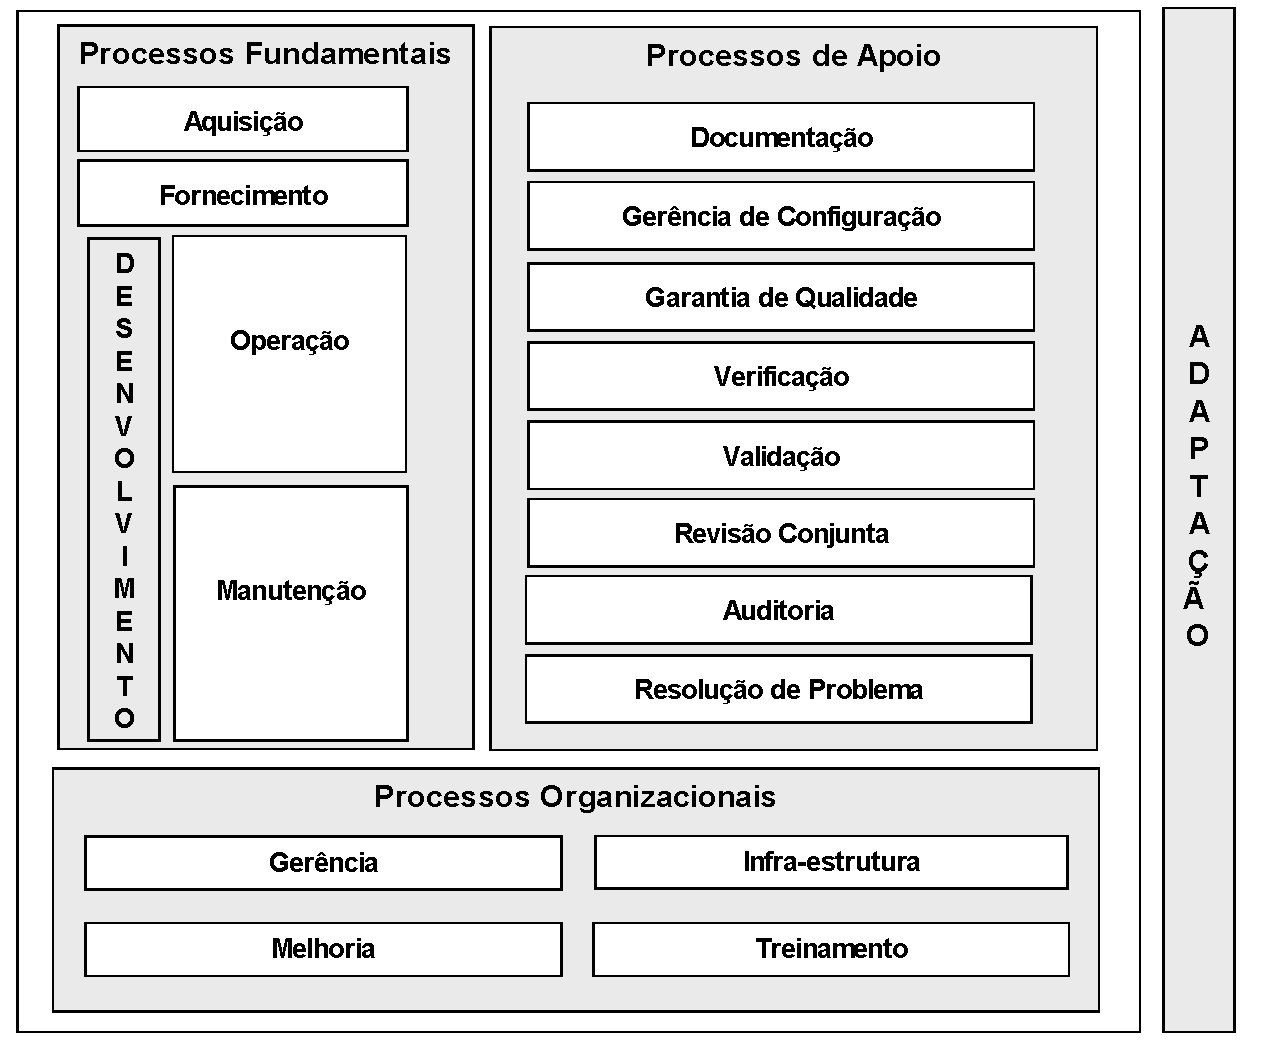
\includegraphics [width=13cm, height=8cm]{12207.pdf}
  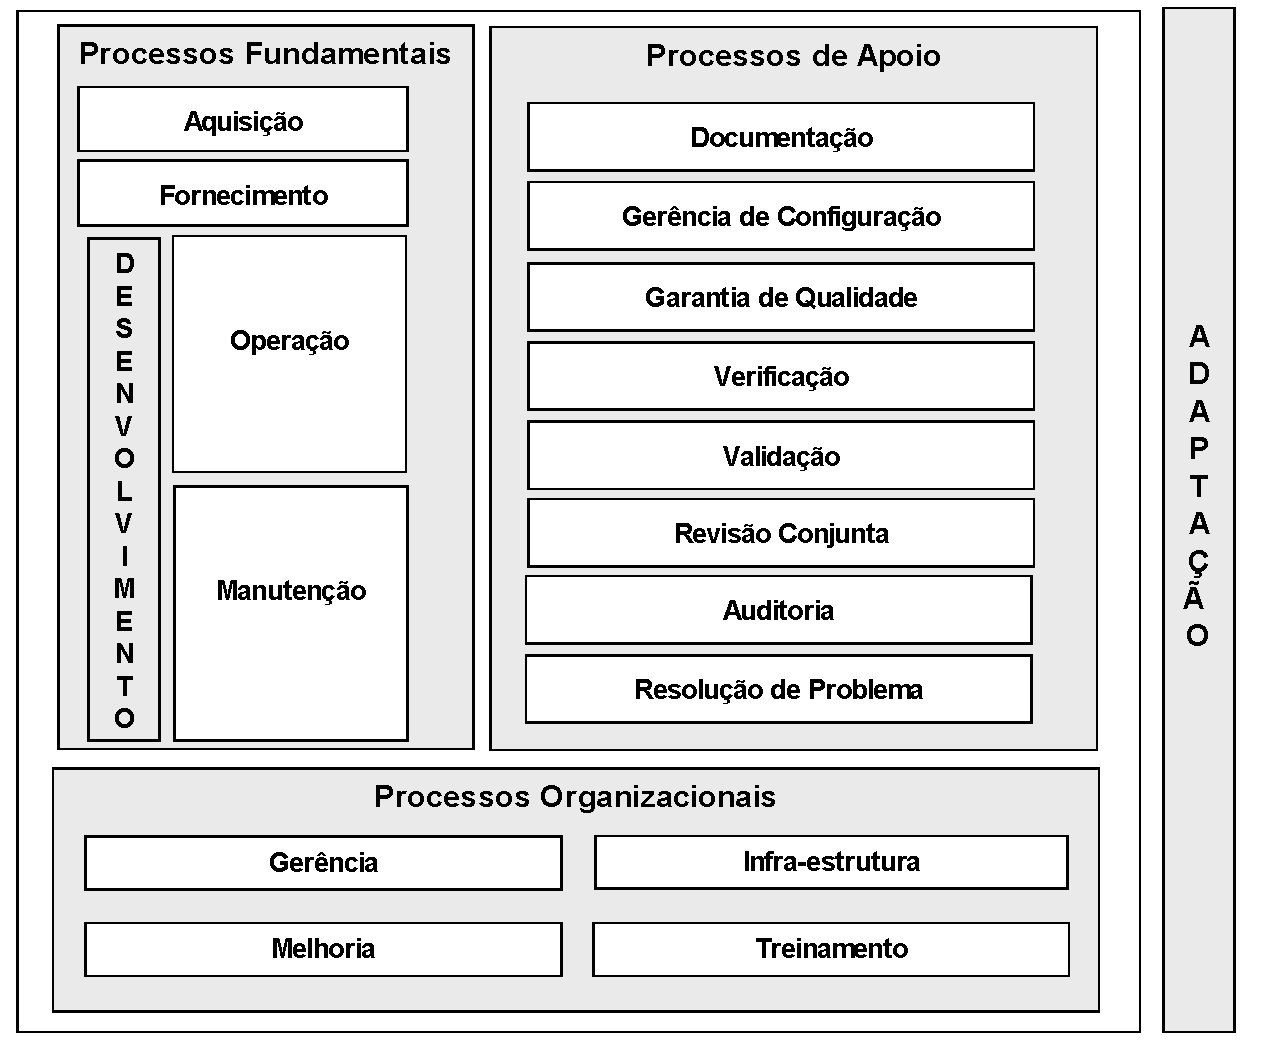
\includegraphics [width=0.9\textwidth]{12207.pdf}
  \caption {Estrutura da Norma \cite{ISO12207}}
  \label{Iso12207}
\end{figure}

Nos \textbf{processos fundamentais} est�o inclu�dos os processos de aquisi��o, de fornecimento, de desenvolvimento, de opera��o e de manuten��o. No processo de aquisi��o � identificada a necessidade de aquisi��o de um sistema, um produto ou um servi�o de software, � preparado e emitido o pedido de proposta e s�o definidos os crit�rios de aceita��o ou rejei��o do item adquirido. No processo do fornecimento s�o realizadas a
prepara��o de uma resposta a um adquirente, a assinatura de um
contrato, a determina��o dos procedimentos e recursos necess�rios
para gerenciar e garantir o projeto e a entrega do sistema. No processo de desenvolvimento s�o definidas as atividades do ciclo de vida de desenvolvimento do software. No processo de opera��o s�o definidas as atividades que ser�o cumpridas para orienta��o ao usu�rio e envio de informa��es para o processo de manuten��o do produto. No processo de manuten��o s�o definidas as atividades que o mantenedor do software dever� cumprir.

Nos \textbf{processos de apoio} est�o inclu�dos o processo de documenta��o, de ger�ncia de configura��o, de garantia de qualidade, processo de verifica��o, processo de valida��o, o processo de revis�o conjunta, processo de auditoria, de resolu��o de problemas. No processo de documenta��o s�o definidas as atividades para planejar, projetar, desenvolver, produzir, editar,
distribuir e manter os documentos. No processo de ger�ncia de configura��o,
os itens de software s�o identificados, as modifica��es, o armazenamento, a manipula��o e
a distribui��o dos itens de software s�o controladas e as vers�es s�o gerenciadas.
No processo de garantia da qualidade, os processos
e produtos de software s�o avaliados em rela��o aos requisitos
e planos. No processo de verifica��o os produtos de software s�o avaliados em rela��o � corretitude t�cnica. No processo de valida��o � avaliado se o produto de software cumpre com o objetivo de uso para o qual foi constru�do. No processo de revis�o, as atividades do processo e os artefatos resultantes s�o avaliados. No processo de auditoria, a adequa��o do produto aos requisitos, aos planos e ao contrato � avaliada. No processo de resolu��o de problemas � definido um processo
para analisar e resolver problemas de qualquer natureza, detectados durante o desenvolvimento, a opera��o, a manuten��o ou o cumprimento de outros processos.

Nos \textbf{processos organizacionais} est�o inclu�dos o processo de ger�ncia, o processo de infra-estrutura, o processo de melhoria e o processo de treinamento. No processo de ger�ncia, s�o definidas as atividades que devem ser cumpridas para gerenciamento do produto, do projeto e das tarefas relacionadas ao
desenvolvimento do software, tais como, aquisi��o, fornecimento,
desenvolvimento, opera��o, manuten��o e apoio. No processo de infra-estrutura s�o definidas as atividades para estabelecer e manter a infra-estrutura que prov� apoio ao
ciclo de vida do software. No processo de melhoria s�o definidas as atividades b�sicas que devem ser
desempenhadas para estabelecer, medir, avaliar, controlar
e melhorar o ciclo de vida do software. No processo de treinamento s�o definidas as atividades para prover
treinamento e manter o pessoal treinado.

No \textbf{processo de adapta��o} s�o definidas as atividades necess�rias para
adaptar a norma a uma organiza��o ou a projetos espec�ficos. As
atividades de adapta��o devem considerar, por exemplo, estrat�gias,
procedimentos, pol�ticas e culturas organizacionais, tamanho,
criticalidade e tipo de sistema, modelo de ciclo de vida do
projeto, caracter�sticas do sistema, riscos, custos e pessoal
envolvidos.

\subsubsection{Modelo CMMI}

O modelo CMMI ({\it Capability Maturity Model Integration}) foi proposto como uma evolu��o dos diversos modelos CMM ({\it Capability Maturity Model}) \citep{PauWebCurChi95} apresentados pelo SEI ({\it Software Engineering Institute}) a partir da d�cada de 1990. O resumo apresentado a seguir foi adaptado de \cite{kos06}.

O objetivo do CMMI � servir de guia para melhoria de processos na organiza��o e tamb�m da habilidade dos profissionais em gerenciar o desenvolvimento, a aquisi��o e a manuten��o de produtos ou servi�os. Assim como no caso do CMM, espera-se que, com o uso do CMMI, a organiza��o seja mais eficiente, respeitando seus pr�prios prazos e construindo software com menos erros.

H� quatro �reas de conhecimento (ou disciplinas) presentes no modelo CMMI: (1) engenharia de sistemas, (2) engenharia de software, (3) desenvolvimento e integra��o de produtos e processos e (4) fontes de aquisi��o. A primeira delas tem por objetivo a obten��o bem sucedida de sistemas, envolvendo software ou n�o. A engenharia de software tem o intuito de disciplinar a produ��o de software. O desenvolvimento e integra��o do produto e do processo � uma abordagem sistem�tica que utiliza a colabora��o dos participantes do projeto para melhor satisfazer as expectativas e requisitos dos clientes. A disciplina de fontes de aquisi��o atua na aquisi��o de produtos ou servi�os para o desenvolvimento dos projetos, pois, � medida que os esfor�os de desenvolvimento aumentam, os projetos podem precisar de fornecedores que realizem fun��es espec�ficas ou prestem manuten��es nos artefatos gerados. 

H� duas representa��es para o CMMI, denominadas representa��o por est�gios e representa��o cont�nua. A abordagem por est�gios segue a mesma estrutura utilizada no CMM, ou seja, as �reas de processo s�o organizadas em cinco n�veis de maturidade para guiar a melhoria de processos. Os n�veis representam um caminho de melhoria de processo para toda a organiza��o. Os n�veis de maturidade sugerem uma ordem para a melhoria dos processos. Para cada n�vel de maturidade existem �reas de processo. Em cada �rea de processo h� objetivos e pr�ticas gen�ricas e espec�ficas.

Na representa��o por est�gios existem cinco n�veis de maturidade: (1) inicial, (2) gerenciado, (3) definido, (4) gerenciado quantitativamente e (5) otimizado. Organiza��es que est�o no n�vel inicial n�o possuem um ambiente est�vel de desenvolvimento de software; no n�vel gerenciado desenvolvem projetos cujos requisitos s�o gerenciados e os processos s�o planejados, medidos e controlados; no n�vel definido os processos s�o padronizados e h� maior consist�ncia nos produtos gerados pela organiza��o; no n�vel gerenciado quantitativamente os processos s�o controlados usando m�todos estat�sticos; no n�vel otimizado os processos s�o continuamente melhorados com base em um entendimento quantitativo das causas comuns de altera��es de desempenho.

%Em cada �rea de processo, os objetivos e as pr�ticas espec�ficas s�o listadas, seguidos por objetivos e pr�ticas gen�ricas. As �reas de processo s�o agrupadas em quatro categorias: ger�ncia de processos, ger�ncia de projeto e engenharia e suporte. As �reas de processo relativas � categoria de ger�ncia de processos cont�m atividades relacionadas para definir, planejar, implantar, monitorar, controlar, medir e melhorar processos. As �reas de processo relativas � categoria de ger�ncia de projeto cont�m as atividades de planejamento, monitoramento e controle do projeto. A categoria de engenharia refere-se �s diversas engenharias, como engenharia de sistemas, engenharia de software e engenharia mec�nica. As atribui��es de fornecer suporte ao desenvolvimento e � manuten��o de produtos s�o relativos � categoria de suporte.

Na representa��o cont�nua existem seis n�veis de capacita��o: (0) incompleto, (1) realizado, (2) gerenciado, (3) definido, (4) gerenciado quantitativamente e (5) otimizado. O n�vel incompleto corresponde ao n�o cumprimento de um processo para o desenvolvimento dos projetos. No n�vel realizado, h� um processo que possui entradas e sa�das bem definidas. No n�vel gerenciado, cada processo cumpre com todos os requisitos do n�vel realizado e, al�m disso, � planejado e executado de acordo com uma pol�tica determinada. No n�vel definido, os processos da organiza��o s�o padronizados. No n�vel gerenciado quantitativamente, os processos s�o controlados usando m�todos estat�sticos. No n�vel otimizado, o foco est� na melhoria cont�nua de desempenho dos processos cumpridos na organiza��o.

%\subsubsection{MPS-BR}

%O MPS.BR (Melhoria de Processo do Software Brasileiro) \citep{mpsbr} est� em desenvolvimento no Brasil desde dezembro de 2003 por membros da ind�stria, do governo e da academia. O objetivo principal � atender micro, pequenas e m�dias empresas de software brasileiras que possuem poucos recursos para melhoria dos processos, mas que percebem a import�ncia relacionada � obten��o de maturidade na execu��o dos processos \citep{mpsclei06}.

%A defini��o do modelo baseia-se em tr�s guias:

%\begin{itemize}

%\item Guia geral: cont�m a descri��o geral do MPS.BR e detalha o modelo de refer�ncia (MR-MPS), seus componentes e as defini��es comuns necess�rias para seu entedimento e aplica��o.

%\item Guia de aquisi��o: cont�m recomenda��es para a aquisi��o de software e servi�os.

%\item Guia de avalia��o: cont�m a descri��o do processo de avalia��o, os requisitos para o avaliador e para a avalia��o, o m�todo e os formul�rios para guiar a avalia��o.

%\end{itemize}

%O MPS.BR foi elaborado considerando como base as normas ISO/IEC 12207, ISO/IEC 15504 e pelo CMMI. Algumas das principais caracter�sticas do modelo s�o:

%\begin{itemize}

%\item possui sete n�veis de maturidade, o que possibilita uma implanta��o mais gradual e adequada a pequenas empresas;

%\item criado para a realidade brasileira, em que o software � desenvolvido por micro, pequenas e m�dias empresas;

%\item possui custo acess�vel;

%\item � realizada avalia��o bienal das empresas;

%\item h� forte intera��o entre universidade e empresa

%\end{itemize}

%No modelo de refer�ncia foram definidos sete n�veis de maturidade: (A) em otimiza��o, (B) gerenciado quantitativamente, (C) definido, (D) largamente definido, (E) parcialmente definido, (F) gerenciado e (G) parcialmente gerenciado. No n�vel parcialmente gerenciado, o foco est� na ger�ncia de projetos e de requisitos. No n�vel gerenciado, o foco est� na garantia de qualidade, na aquisi��o de produtos ou servi�os, na ger�ncia de configura��o e na medi��o. No n�vel parcialmente definido, o foco est� na adapta��o do processo para ger�ncia de projeto, na defini��o do processo organizacional, na avalia��o e melhoria do processo organizacional e no treinamento. No n�vel largamente definido, o foco est� no desenvolvimento de requisitos, na solu��o t�cnica, na valida��o, na verifica��o e na integra��o do produto.
%No n�vel parcialmente definido o foco est� na ger�ncia de riscos e na an�lise de decis�o e resolu��o. No n�vel gerenciado quantitativamente o foco est� na ger�ncia quantitativa do projeto e no desempenho do processo organizacional. No n�vel em otimiza��o, o foco est� na an�lise de causas e resolu��es e inova��o e implanta��o na organiza��o.

\section{Processos e ambientes para desenvolvimento de projetos de pesquisa} \label{pp}

Conforme apresentado por \cite{Amb04}, as caracter�sticas
especiais do desenvolvimento de projetos de pesquisa, tais como a
prototipa��o r�pida e a alta rotatividade dos participantes
representam elementos fundamentais que imp�em uma revis�o das
pr�ticas de Engenharia de Software para atender �s necessidades do
contexto de desenvolvimento de pesquisas. Em geral, espera-se que
um processo cumprido em ambiente de pesquisa valorize,
principalmente, a comunica��o entre os membros dos projetos, as
atividades de prototipa��o e de gerenciamento de tarefas, a
defini��o de cronograma, o planejamento de recursos e as
atividades de qualidade de software, envolvendo documenta��o,
gerenciamento de configura��es e testes
\citep{Rob98,seg05,PaulaFilho01}.

Nos �ltimos anos, foram apresentadas propostas de 
processos com o objetivo de atender ao desenvolvimento
de projetos de pesquisa. Embora estejam sendo obtidos resultados
importantes, na pr�tica, ainda � comum que os prot�tipos
desenvolvidos sejam re-escritos por diferentes pessoas, v�rias
vezes, devido �s dificuldades de manuten��o e reuso, acarretando
em preju�zos � evolu��o de pesquisas cient�ficas \citep{Bol04}.

Nas se��es seguintes s�o descritas as propostas que foram encontradas na
literatura sobre processos para o desenvolvimento de projetos de
pesquisa, considerando-se seus aspectos positivos e negativos. Na
Se��o \ref{arte} � apresentada uma an�lise comparativa entre as propostas e
o processo apresentado neste trabalho.

%Um resumo das propostas apresentadas na literatura sobre processos para o desenvolvimento de projetos de pesquisa � apresentado a seguir:

\subsection{{\it eXtreme Researching}} \label{xr}

\cite{Oli05} propuseram uma adapta��o da metodologia XP, denominada {\it eXtreme Researching} (XR), para
desenvolvimento de projetos de pesquisa. A proposta adota e
estende as principais pr�ticas de XP e mostra como podem ser
aplicadas em projetos distribu�dos que envolvem o desenvolvimento
de pesquisas (foi considerado como requisito fundamental para a
elabora��o da proposta que o desenvolvimento de pesquisas ocorre
de forma distribu�da). Os autores consideram que um dos principais
desafios, neste contexto, � propor uma metodologia que
valorize a disciplina em termos de atividades e artefatos e, ao
mesmo tempo, a criatividade dos pesquisadores.
%o desenvolvimento de pesquisas est� fortemente relacionado com prototipa��o r�pida, cujos conceitos devem ser explorados

Foi adotada uma metodologia �gil como base para a proposta devido
a suas principais propriedades, ou seja, s�o orientadas a pessoas,
ao inv�s de serem orientadas a processos; s�o adaptativas, ao
inv�s de serem preditivas ou impositivas e consideram que os
requisitos do software s�o descobertos � medida que o projeto �
desenvolvido. Os autores consideraram que h� uma rela��o entre
estas propriedades e o ambiente de desenvolvimento de projetos de
pesquisa.

Para a elabora��o da proposta foi considerado, al�m da metodologia
XP, o trabalho desenvolvido por \cite{kir01}, que prop�s uma
abordagem para cumprimento das pr�ticas originais de XP de forma
distribu�da. Um dos principais elementos tratados pelos autores
foi a comunica��o entre os membros dos projetos, tendo sido
proposto o uso de ferramentas de {\it email}, teleconfer�ncia e
videoconfer�ncia. Assim, ao adotar os resultados do trabalho de
Kircher et al, a aplica��o da metodologia XR fica restrita a
grupos que possuam a infra-estrutura e os recursos necess�rios
para o estabelecimento da comunica��o de acordo com a proposta (na
pr�tica, nem todas as ferramentas sugeridas s�o amplamente
difundidas). Na Tabela \ref{xr1} s�o apresentadas as pr�ticas de XR que foram
propostas. 

\begin{table}[!h]
\begin{center}
\caption{Pr�ticas da metodologia XR \citep{Oli05}}\label{xr1}
%\begin{tabular}{|p{3.2cm}|p{10.5cm}|}
%\begin{tabularx}{0.75\textwidth}{|l|l|}
\begin{tabular}{|p{5.8cm}|p{9cm}|}
\hline
\footnotesize 
\begin{center}
\textbf{Atividade}
\end{center}
 & \footnotesize 
\begin{center}
\textbf{Descri��o e Informa��es Gerais}
\end{center}
\\
\hline
\hline \footnotesize \sffamily Integra��o frequente & \footnotesize Realizada por meio do uso de um reposit�rio {\it online}, sempre dispon�vel para membros dos grupos. N�o h� uma fase de integra��o espec�fica. Pesquisadores desenvolvendo uma prova de conceito esperam obter {\it feedback} r�pido do c�digo para refinar uma primeira id�ia  \\
\hline \footnotesize \sffamily Programa��o por pares remotos & \footnotesize Executada a partir do compartilhamento da �rea de trabalho e comunica��o via rede de computadores \\
\hline \footnotesize \sffamily Cliente dispon�vel & \footnotesize O principal pesquisador (ou coordenador do projeto) cumpre o papel de cliente e toma as decis�es de projeto. Os requisitos s�o discutidos pelos membros dos grupos de pesquisa   \\
\hline \footnotesize \sffamily Conhecimento coletivo & \footnotesize Os grupos de pesquisa mant�m uma base de conhecimento coletiva e fazem refer�ncias constantes ao reposit�rio \textit{online} (inclus�o, altera��o e exclus�o de documentos) \\
\hline \footnotesize \sffamily Jogo do planejamento & \footnotesize A comunica��o s�ncrona e ass�ncrona entre os membros que participam do projeto � fundamental para o cumprimento desta pr�tica. Pode ser precedido por um jogo de met�foras ou por um {\it brainstorming}, que ajudam definir e priorizar o que precisa ser implementado (refinar e definir as est�rias dos usu�rios)\\
\hline \footnotesize \sffamily Met�fora & \footnotesize S�o utilizadas para gerar est�rias dos usu�rios. Evoluem enquanto o c�digo est� sendo escrito \\
\hline \footnotesize \sffamily Quarenta horas por semana & \footnotesize Al�m das atividades de desenvolvimento dos projetos, os pesquisadores possuem muitas outras tarefas, por exemplo, redigir documentos t�cnicos, solicitar financiamento � ag�ncias de fomento, etc. Como resultado, o n�mero de horas de trabalho por semana pode variar consideravelmente\\
\hline \footnotesize \sffamily Padr�es de c�digo & \footnotesize O uso de padr�es de c�digo � fundamental para disciplinar o desenvolvimento de projetos por grupos. Pode ser considerado como um dos fatores que torna o software mais compreens�vel \\
\hline \footnotesize \sffamily Pontos de controle  & \footnotesize Definindo-se pontos de controle, as diverg�ncias dos principais objetivos de pesquisa podem ser analisadas periodicamente e decis�es s�o tomadas considerando-se o contexto geral dos projetos\\
\hline \footnotesize \sffamily Testes & \footnotesize Testes de unidade s�o executados, como acontece em XP, para assegurar a qualidade e a validade dos resultados de pesquisa\\
\hline \footnotesize  \sffamily Refatoramento & \footnotesize Ocorre ao final de cada itera��o de desenvolvimento\\
\hline \footnotesize \sffamily Modelagem baseada em componentes & \footnotesize Promove a disponibiliza��o do conhecimento sobre o projeto aos grupos\\
\hline
\hline
\end{tabular}
\end{center}
\end{table}


Foi apresentado tamb�m um portal {\it web}, denominado XPWeb\footnote{http://sourceforge.net/projects/xpweb}, que oferece apoio ao
desenvolvimento de projetos utilizando XP e disponibiliza os
reposit�rios necess�rios para o desenvolvimento de projetos de
acordo com a abordagem XR. O principal objetivo do portal �
fornecer um conjunto de ferramentas que promova o compartilhamento
de conhecimento em um ambiente distribu�do e seja �til para o desenvolvimento de
provas de conceito. Outra caracter�stica importante � que o portal
possui interfaces para v�rios sistemas, como CVS\footnote{Concurrent
Versions System; http://www.nongnu.org/cvs/}, {\it Rational Rose}\footnote{http://www-306.ibm.com/software/rational/} e o {\it framework} de testes xUnit\footnote{http://www.junit.org/index.htm}. Pretende-se
incluir, ainda, ferramentas de rastreamento de bugs ({\it bug
trackers}), ferramentas de aux�lio � vota��o, dentre outras. Mais
recentemente foi disponibilizado o EcliXPWeb\footnote{http://sourceforge.net/projects/eclixpweb}, que � um {\it
plug-in} para o ambiente Eclipse\footnote{www.eclipse.org} e que faz refer�ncias �s bases de dados do
XPWeb. Na Figura \ref{portal} � apresentada uma  tela do portal,
utilizada para a execu��o de testes de unidade.


\begin{figure} [!ht]
 \centering
  \bfseries
  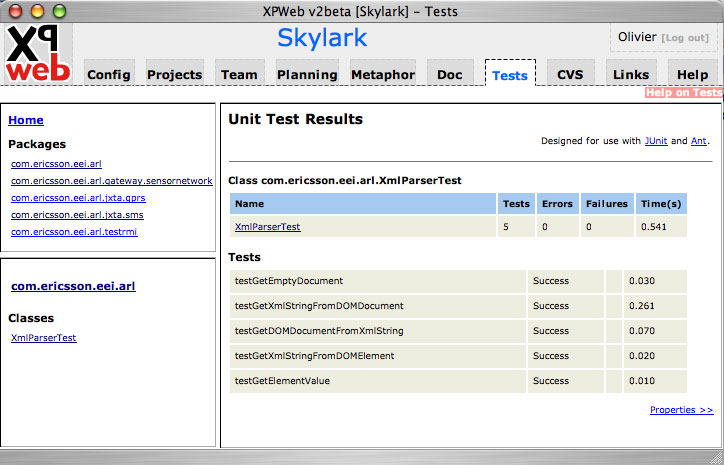
\includegraphics [width=0.95\textwidth]{XPWeb.jpg}
  \caption{Portal XPWeb desenvolvido de acordo com a abordagem XR}
  \label{portal}
\end{figure}

Podem ser destacados como elementos favor�veis � abordagem XR:
\begin{enumerate}
\item 
o fato de considerar o desenvolvimento de projetos distribu�dos,
que est� sendo observado como uma tend�ncia em termos de projetos
de software no geral (Se��o \ref{historico}) e � um requisito em
termos de processos para o desenvolvimento de pesquisas; 
\item  o desenvolvimento e a
evolu��o de um portal que oferece suporte ao cumprimento das
pr�ticas e integra ferramentas que auxiliam a execu��o de
diferentes atividades do processo 
\item  est� baseado em uma
metodologia difundida (XP), conhecida pela comunidade cient�fica.
\end{enumerate}

Como elementos desfavor�veis, observa-se que: 

\begin{enumerate}
\item  n�o foram
indicadas as atividades a serem cumpridas e os artefatos a serem
gerados; 
\item n�o foi indicado como s�o tratados elementos
fundamentais de sistemas distribu�dos, por exemplo, direitos de
acesso e pol�ticas de uso de um reposit�rio de dados 
\item a
proposta trata, fundamentalmente, de um modelo de ciclo de vida
para desenvolvimento de projetos de pesquisa. H� poucas
refer�ncias � atividades de garantia de qualidade, atividades de
apoio organizacional.
\end{enumerate}

\subsection{Processo padr�o para pesquisa e desenvolvimento} \label{pad}

Foi proposto em 2006 um processo padr�o para pesquisa e
desenvolvimento por pesquisadores do Instituto de Pesquisas em
Telecomunica��es e Eletr�nica na Korea \citep{Hwa06}. Padr�es
internacionais para Engenharia de Sistemas e Engenharia de
Software e a pr�pria experi�ncia dos pesquisadores foram considerados.

Conforme apresentado na Figura \ref{kor}, o processo �
composto por 41 sub-processos, divididos em quatro categorias que
s�o: (1) processos de ciclo de vida para projetos de pesquisa e
desenvolvimento, (2) processos de suporte, (3) processos de gerenciamento
de projetos e (4) processos organizacionais. A primeira categoria �
dividida em cinco sub-categorias, que s�o: sistemas/software,
dispositivos, tecnologias, padr�es, pol�ticas e estrat�gias. O
objetivo desta categoria � auxiliar o desenvolvimento de produtos
que cumpram os requisitos dos clientes. A categoria de processos
de suporte foi proposta para assegurar a integridade dos artefatos
produzidos durante o desenvolvimento do projeto. A categoria de
processos de gerenciamento de projetos estabelece os planos de
projeto que precisam ser elaborados e avalia os resultados e os
progressos obtidos em rela��o aos planos. A categoria de processos
organizacionais estabelece os objetivos de neg�cios relacionados
ao projeto e prop�e atividades que ajudem a alcan�ar tais
objetivos.

\begin{figure} [!ht]
 \centering
  \bfseries
  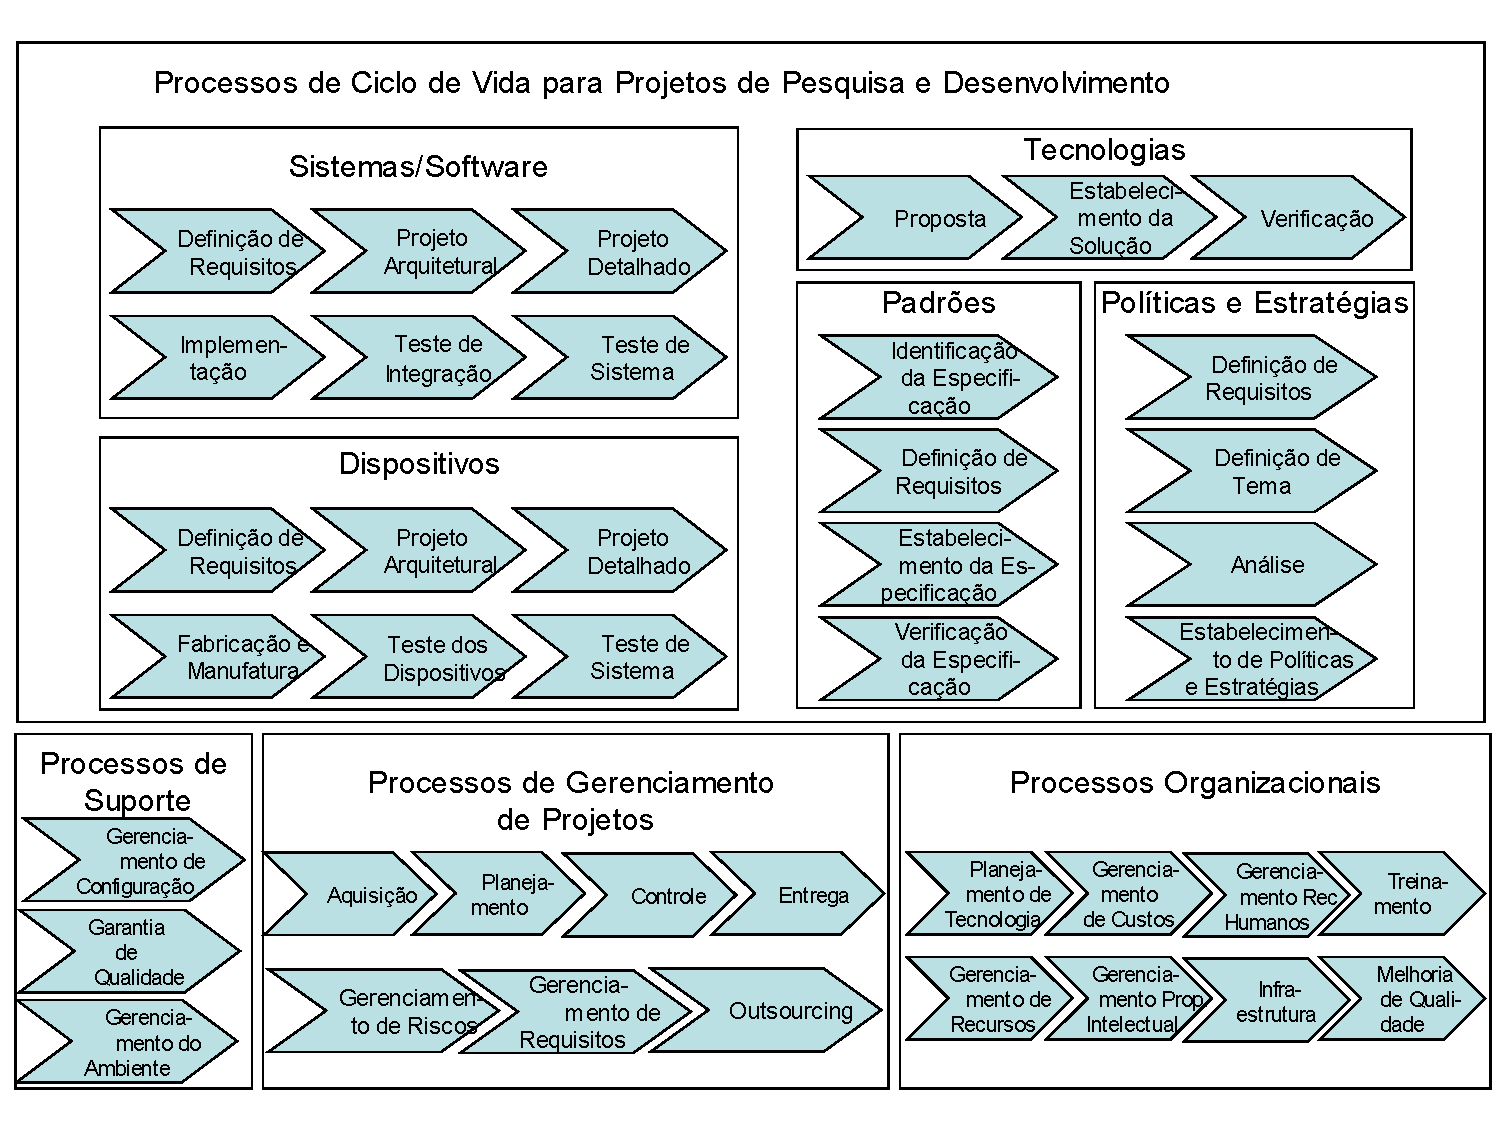
\includegraphics [width=0.95\textwidth]{processo_koreano.pdf}
  \caption{Vis�o geral do processo para pesquisa e desenvolvimento proposto por \cite{Hwa06}}
  \label{kor}
\end{figure}

%O processo proposto foi comparado com a Norma ISO/IEC 15288 \citep{ISO15288}, que � um padr�o internacional que foi publicado em 2002 com o objetivo de integrar elementos de engenharia de software e engenharia de sistemas, podendo ser considerada como uma evolu��o da Norma \cite{ISO12207}. Como resultado da compara��o realizada, destaca-se que os processos de manuten��o e interrup��o do projeto, sugeridos na norma, n�o foram considerados devido �s caracter�sticas dos projetos desenvolvidos no instituto para o qual a pesquisa estava sendo realizada. Por outro lado, o processo de gerenciamento de propriedade intelectual � um processo que n�o estava contido na norma e que foi inclu�do processo proposto.

%Na pr�tica, a aplica��o de atividades de processos de software no contexto de desenvolvimento de pesquisas � frequentemente ca�tico. Como resultado, de acordo com Boldyreff et al \cite{Bol04}, � comum que as funcionalidades dos projetos de pesquisa sejam re-implementadas, ao inv�s de evolu�rem.

Observa-se, como um dos principais \textit{pontos favor�veis}, que o processo proposto � amplo no sentido de englobar n�o somente atividades de ciclo de vida, mas tamb�m atividades de Engenharia de Software e Engenharia de Sistemas. Al�m disso, foram considerados interesses do setor industrial para a elabora��o da proposta, cobrindo um dos principais requisitos de um processo para o desenvolvimento de projetos de pesquisa, que est� relacionado � participa��o do setor industrial no desenvolvimento de pesquisa (discutido na Se��o \ref{obj}).  

Pode ser mencionado, como \textit{ponto desfavor�vel}, o fato de a proposta estar direcionada a um determinado contexto. N�o foram considerados trabalhos de outros pesquisadores (estado da arte), nem requisitos apresentados na literatura sobre processos para pesquisa e desenvolvimento. Uma consequ�ncia disso � que processos considerados fundamentais por outros autores, por exemplo, aqueles relacionados � manuten��o dos projetos e a colabora��o entre os membros, n�o foram inclu�dos. Finalmente, n�o foram apresentadas informa��es sobre as possibilidades e as restri��es da generaliza��o da proposta para outros ambientes diferentes daquele para o qual a proposta foi elaborada. %Al�m disso, a descri��o do processo n�o est� amplamente dispon�vel, o que dificulta sua ado��o e avalia��o.


\subsection{HDG ({\it Higher Degree Process})}

O HDG \citep{wal03} foi proposto por pesquisadores do SEAL ({\it
Software Engineering Applications Laboratory}), da �frica do Sul,
com o objetivo de ser utilizado como um modelo de refer�ncia para
a realiza��o de avalia��es dos processos cumpridos no pr�prio
laborat�rio. � interessante notar o interesse dos pesquisadores
com a qualidade e a melhoria dos processos cumpridos no
laborat�rio. Ap�s conseguir a certifica��o da norma \cite{ISO9001}, em 1995, tiveram a iniciativa de avaliar seus
processos de acordo com as recomenda��es da norma ISO/IEC 15504 (e
para isso propuseram o HDG). Em 2001, por exemplo, foi alcan�ado o
n�vel 3 para alguns dos processos cumpridos no laborat�rio. Poucos
anos depois foi alcan�ado o n�vel 5 para outros processos. O HDG
foi um dos resultados obtidos com os esfor�os de melhoria de
processos de software no contexto do SEAL. As pr�ticas base que
comp�em o processo s�o apresentadas na Tabela \ref{hdp}.

\begin{table}[!h]
\begin{center}
\caption{Pr�ticas base do HDG \citep{wal03}}\label{hdp}
%\begin{tabular}{|p{3.2cm}|p{10.5cm}|}
\begin{tabularx}{0.95\textwidth}{|X|}
\hline \footnotesize {\bf \sffamily HDG.PB1 -- Definir os objetivos do projeto de pesquisa:} \normalfont definir uma proposta de projeto de pesquisa, indicando os objetivos, os principais requisitos, os recursos necess�rios, os prazos, os requisitos t�cnicos, os requisitos de qualidade de processos e os produtos de trabalho que dever�o ser gerados  \\
\hline \footnotesize {\bf \sffamily HDG.PB2 -- Planejar a pesquisa:} \normalfont identificar as entradas necess�rias, as atividades a serem cumpridas, os recursos, os prazos associados �s atividades, as responsabilidades dos membros e os relat�rios necess�rios\\
\hline \footnotesize {\bf \sffamily HDG.PB3 -- Determinar as condi��es t�cnicas:} \normalfont revisar a literatura t�cnica e avaliar o impacto do projeto\\
\hline \footnotesize {\bf \sffamily HDG.PB4 -- Realizar revis�o detalhada dos objetivos t�cnicos do projeto:} \normalfont revisar o impacto do resultado da revis�o da literatura nos objetivos do projeto, atualizando o plano, se necess�rio\\
\hline \footnotesize {\bf \sffamily HDG.PB5 -- Desenvolver o projeto de pesquisa:} \normalfont cumprir as atividades apresentadas no plano de projeto\\
\hline \footnotesize {\bf \sffamily HDG.PB6 -- Revisar e aprovar os resultados:} \normalfont o coordenador do projeto e os pesquisadores revisam os produtos de trabalho resultantes do cumprimento das atividades propostas. Os produtos s�o aprovados quando os objetivos s�o alcan�ados e os crit�rios de qualidade s�o satisfeitos.\\
\hline \footnotesize {\bf \sffamily HDG.PB7 -- Validar os resultados da pesquisa em rela��o a proposta:} \normalfont assegurar que os produtos de trabalho resultantes do projeto de pesquisa cumprem os requisitos t�cnicos\\
\hline \footnotesize {\bf \sffamily HDG.PB8 -- Disseminar os resultados da pesquisa:}\normalfont  apresentar os resultados da pesquisa no formtato de artigos t�cnicos, de forma que possam ser revisados, apresentados em confer�ncias e reuni�es t�cnicas e publicados em meios reconhecidos. \\
\hline \footnotesize {\bf \sffamily HDG.PB9 -- Redigir a disserta��o ou a tese:} \normalfont produzir o documento de disserta��o ou tese a partir dos produtos de trabalho do projeto\\
\hline \footnotesize {\bf \sffamily HDG.PB10 -- Avaliar os resultados do projeto de pesquisa em rela��o aos requisitos de avalia��o:}\normalfont  a disserta��o e a tese s�o avaliadas em rela��o aos requisitos iniciais do projeto\\
\hline
\end{tabularx}
\end{center}
\end{table}

Como \textit{ponto favor�vel} ao processo proposto, pode-se destacar o fato de o
autor ter apresentado os processos indicando atividades e
artefatos que s�o intr�nsecos ao desenvolvimento de pesquisas.
Outra parte do processo apresentado, que complementa as pr�ticas
base, se refere � descri��o de um conjunto de problemas que
geralmente ocorrem no desenvolvimento de pesquisas (por exemplo, o
pequeno n�mero de publica��es obtidas como resultado dos projetos
de pesquisa) e oportunidades de melhoria. As a��es sugeridas s�o
bastante simples e, adot�-las na pr�tica pode ser muito �til para
dar in�cio a programas de melhoria de processos em outras
institui��es ou grupos de pesquisa. 

Como \textit{fator desfavor�vel} pode-se
citar a descri��o bastante gen�rica da proposta. N�o foram
apresentados detalhes sobre o cumprimento das pr�ticas base (devem
ser cumpridas sequencialmente? de forma iterativa? s�o compostas
por quais atividades?) e dos artefatos a serem elaborados.

\subsection{A proposta de Nunamaker e Chen}

\cite{numa90} propuseram um processo para desenvolvimento de
sistemas de informa��o no contexto de projetos de pesquisa. Para a
elabora��o da proposta, os autores consideraram a import�ncia em
integrar elementos de metodologia de pesquisa em um {\it framework},
abrangendo o desenvolvimento de um sistema. Uma vis�o geral da proposta � apresentada na Figura
\ref{numa}.

\begin{figure} [!ht]
 \centering
  \bfseries
  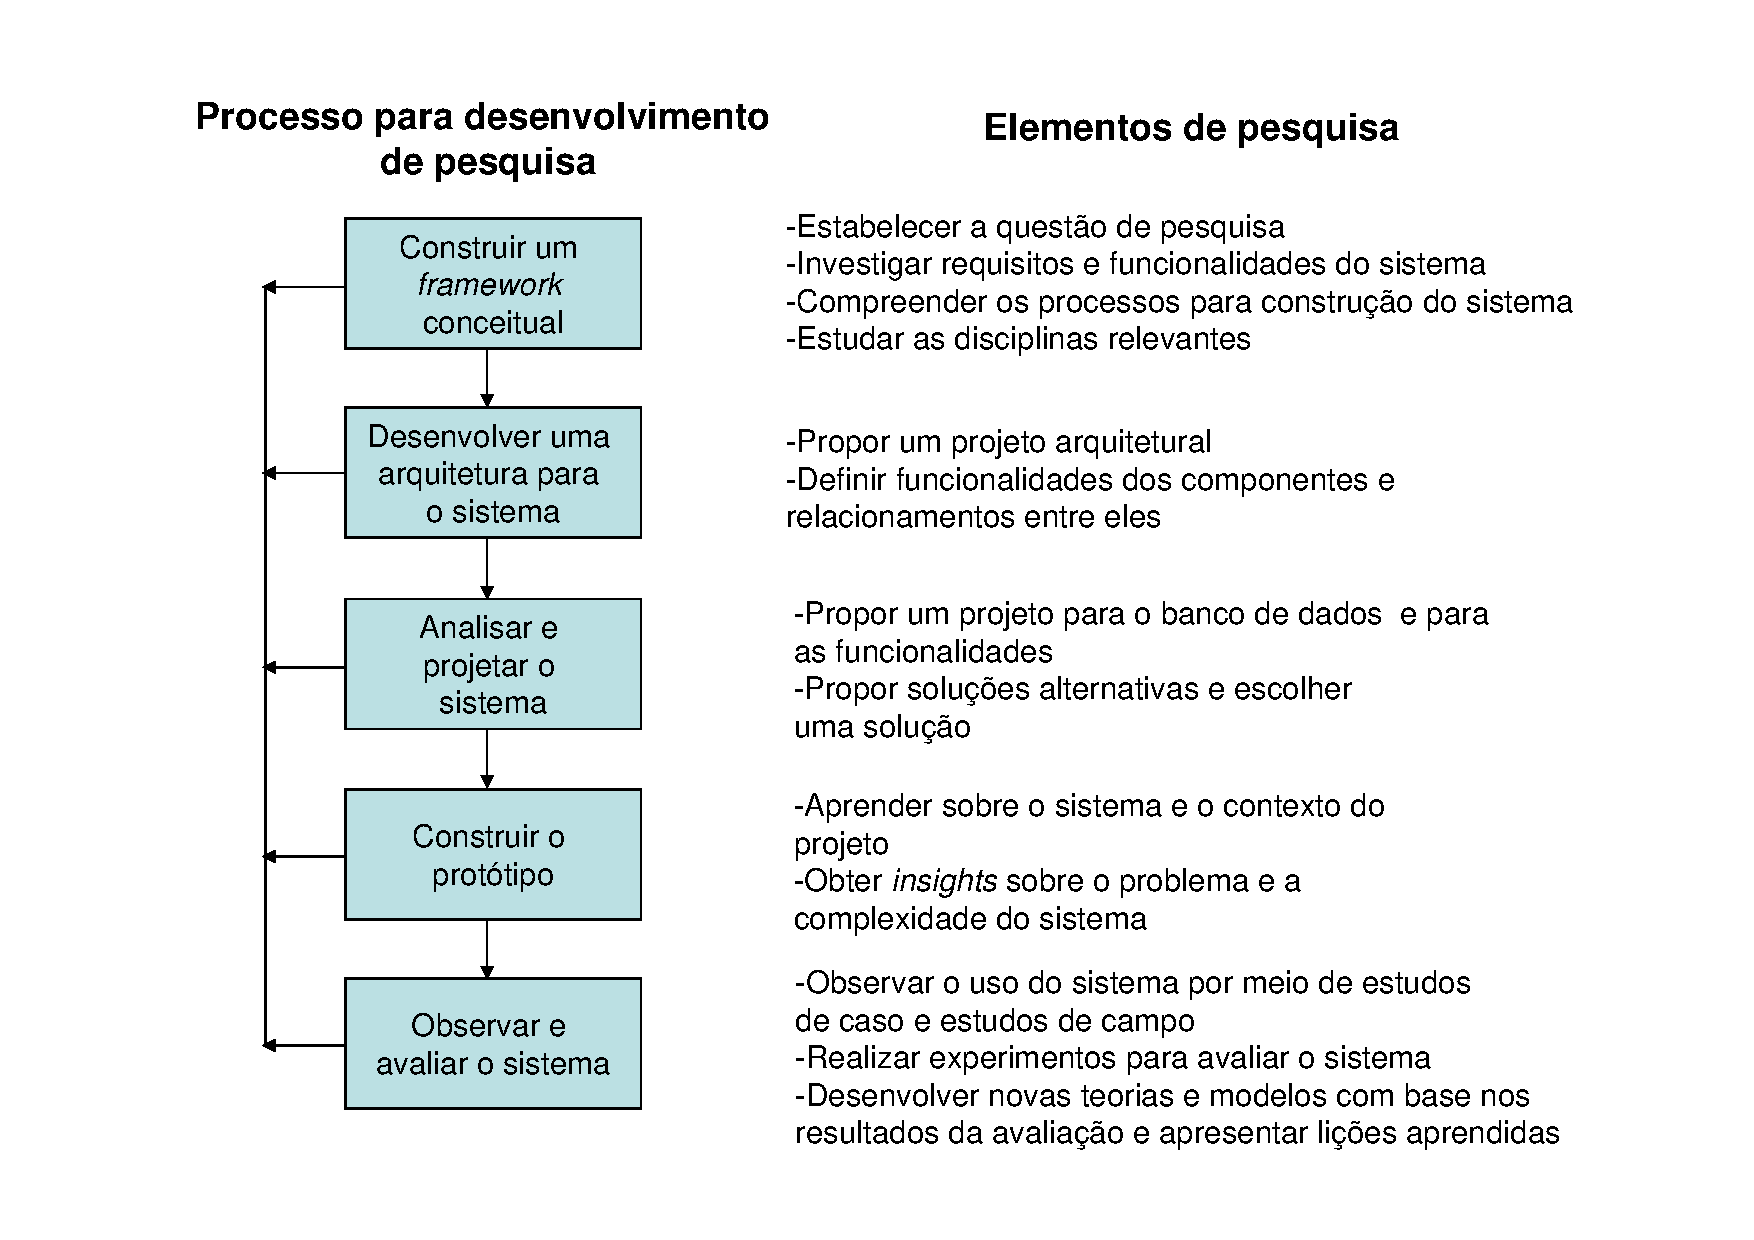
\includegraphics [width=0.95\textwidth]{processo_numpra.pdf}
  \caption{Processo para desenvolvimento de projetos de pesquisa proposto por \cite{numa90}}
  \label{numa}
\end{figure}

Para a fase de constru��o de um {\it framework} conceitual, os
autores sugerem que os pesquisadores avaliem o quanto a quest�o de
pesquisa � significativa. Al�m disso, devem ser discutidas as abordagens que ser�o usadas para resolver o problema. Na fase de
elabora��o da arquitetura, � importante
apresentar o sistema sob uma perspectiva de componentes,
especificar suas funcionalidades e definir a estrutura e
as intera��es din�micas entre os componentes. Na fase
de an�lise e projeto do sistema deve-se compreender o dom�nio do
problema, observar a possibilidade de aplica��o de conhecimento
t�cnico e cient�fico relevante e as alternativas para o projeto. Na fase
de constru��o do prot�tipo, a implementa��o do sistema � realizada
para demonstrar a viabilidade do projeto de pesquisa. Na fase de
observa��o e avalia��o do sistema, os pesquisadores avaliam o
desempenho e a usabilidade do sistema conforme definido nas fases
iniciais do desenvolvimento.

O principal \textit{fator positivo} observado na proposta de Nunamaker \&
Chen � a integra��o de elementos de metodologia para
desenvolvimento de projetos de pesquisa. Considerando-se que a
proposta foi apresentada no come�o da d�cada de 1990, nota-se que
foi uma iniciativa importante no sentido de divulgar elementos de
metodologia cient�fica no contexto de um processo para 
desenvolvimento de projetos de pesquisa. O principal \textit{fator
negativo} observado � a aus�ncia de contextualiza��o da proposta,
ou seja, n�o foram mencionados os requisitos considerados na
elabora��o da proposta e como a avalia��o foi realizada. Nota-se,
ainda, que o processo cobre apenas atividades de 
desenvolvimento e n�o faz refer�ncia a atividades como
gerenciamento de projetos e garantia de qualidade. Tamb�m n�o �
mencionada a possibilidade de desenvolver projetos distribu�dos e
colaborativos, que s�o tend�ncias em termos de desenvolvimento de
pesquisas, usando a abordagem proposta.

%\subsection{O processo utilizado no CERN}

%Alguns relatos foram apresentados na literatura sobre experi�ncias envolvendo a aplica��o de pr�ticas de Engenharia de Software no desenvolvimento de projetos de pesquisa \cite{seg05,cav89}. Apesar de n�o ter sido definido um processo espec�fico, considerando as caracter�sticas inerentes deste tipo de desenvolvimento, as experi�ncias apresentadas foram importantes no sentido de indicar as necessidades dos autores em rela��o aos processos, �s atividades e aos artefatos, ou seja, foram indicados requisitos para um processo que s�o �teis ao desenvolvimento de projetos de pesquisa. Esses requisitos ser�o apresentados na Se��o X.

%Uma experi�ncia interessante em rela��o � aplica��o de pr�ticas de
%Engenharia de Software no desenvolvimento de pesquisas foi
%relatada por Walker \cite{wal03}. Os esfor�os concentrados na
%melhoria dos processos cumpridos no {\it Software Engineering
%Applications Laboratory} resultaram na obten��o de importantes
%certifica��es. Muitas li��es foram aprendidas com esta experi�ncia
%e os autores destacam como importantes fatores de sucesso o
%gerenciamento cont�nuo dos projetos e a documenta��o subjacente.

\subsection{{\it Collaboratories}}

De forma geral, {\it collaboratories} est�o relacionados ao uso de tecnologias de colabora��o para apoiar o desenvolvimento de pesquisas cient�ficas geograficamente distribu�das. Formalmente, s�o definidos como ``um centro sem paredes'', em que pesquisadores podem desenvolver suas pesquisas sem se preocupar com a localiza��o geogr�fica. Pesquisadores registraram li��es aprendidas como resultados de suas experi�ncias com {\it collaboratories} e indicaram atividades e ferramentas que consideram importantes para este contexto, conforme apresentados a seguir:


\begin{itemize}

\item \cite{ols02} apresentaram tr�s elementos que consideram fundamentais para que a colabora��o (e a implanta��o de {\it collaboratories}) possa ocorrer: motiva��o das pessoas envolvidas para o trabalho em equipe, colabora��o constante e disponibilidade de infra-estrutura e de ferramentas. Os autores destacaram como li��es aprendidas a import�ncia em (1) usar uma abordagem iterativa, em que os ciclos de desenvolvimento envolvam as fases de projeto, desenvolvimento, implanta��o e avalia��o; (2) prover e utilizar ferramentas que promovam a participa��o dos membros em semin�rios e reuni�es de laborat�rios virtuais (3) discutir normas �ticas das comunidades ou pa�ses participantes e (4) oferecer treinamento sobre ferramentas e tecnologias antes que sejam adotadas para uso. Os autores experimentaram diferentes ferramentas em suas experi�ncias em {\it collaboratories} e destacaram as seguintes: Microsoft NetMeeting\footnote{{http://www.microsoft.com/windows/netmeeting/}}, Timbuktu Conference\footnote{(http://www.netopia.com/software/products/tb2/)} e Virtual PC\footnote{(http://www.apple.com/macosx/applications/virtualpc/)}.

\item \cite{dia03} realizaram experimentos em {\it collaboratories} e indicaram atividades que consideraram ser primordiais a partir do estudo que realizaram: fornecer canais redundantes para promover a comunica��o, fornecer m�ltiplas formas para visualiza��o de v�deo, compartilhar instrumenta��o cient�fica, fornecer canais satisfat�rios para transmiss�o de �udio, fornecer informa��es sobre o que os membros do projeto est�o fazendo, oferecer dicas sobre o {\it status} dos membros em rela��o � comunica��o (por exemplo, se est�o {\it online} ou {\it offline}),


\item O trabalho de \cite{Far05} tamb�m deve ser mencionado, pois nele, foi investigada a rela��o entre criatividade, que � um aspecto central do desenvolvimento de pesquisas, e o suporte � colabora��o por meio de ferramentas. Como um dos resultados da pesquisa, foi proposto um prot�tipo para ser usado em ambiente de {\it collaboratories} denominado BRIDGE ({\it Basic Resources for Integrated Distributed Group Environments}\footnote{http://bridgetools.sourceforge.net}). O prot�tipo disponibiliza funcionalidades para troca de mensagens, suporte � gera��o de gr�ficos, suporte a {\it social awareness} e {\it workspace awareness} e coordena��o e planejamento dos projetos. Al�m disso, h� dispon�vel uma linha de tempo ({\it timeline}) em que � indicado o hist�rico do projeto e os {\it deadlines} importantes. O sistema apresenta uma integra��o entre os gr�ficos, os documentos e a linha de tempo.

\end{itemize}

O objetivo dos {\it collaboratories} � permitir que cientistas que est�o geograficamente dispersos possam trabalhar de forma colaborativa, usando tecnologias apropriadas para acessar ferramentas, bancos de dados e instrumentos uns dos outros \citep{wul89,kou96}. Assim, esse objetivo � um fator \textit{positivo} da iniciativa. 

No entanto, como fator \textit{negativo}, n�o foi encontrado na literatura um processo, envolvendo atividades, infra-estrutura e gerenciamento de recursos, que tenha sido proposto para {\it collaboratories} e que tenha sido avaliado.

\section{Considera��es finais}

Neste cap�tulo buscou-se apresentar as principais abordagens em termos de processsos de software e modelos de qualidade que foram importantes como fundamenta��o obtida da literatura cient�fica para o desenvolvimento deste trabalho. Os processos para desenvolvimento de software s�o relevantes neste contexto, pois considera-se que um dos artefatos essenciais que permitem a realiza��o de provas de conceito em termos de pesquisas � o software, o prot�tipo que tenha sido constru�do de forma dedicada ao projeto de pesquisa. 

Al�m disso, os processos cumpridos para desenvolvimento de projetos distribu�dos e colaborativos, os processos de software livre e as metodologias �geis tamb�m fornecem elementos que foram importantes para o desenvolvimento deste trabalho e, portanto, foram descritos. Por fim, foram apresentados os trabalhos encontrados na literatura que tiveram a �nfase em processos para desenvolvimento de projetos de pesquisa.  

\chapter{Revis�o Bibliogr�fica: {\it Design Rationale}} \label{cap_DR}

\section{Considera��es iniciais}

Neste cap�tulo s�o apresentados conceitos sobre {\it design rationale}, considerando-se suas principais perspectivas e as atividades de captura, representa��o e recupera��o das informa��es. Foram enfatizados tamb�m os trabalhos de pesquisa apresentados na literatura, com o objetivo de apresentar os principais resultados que j� foram obtidos e as principais tend�ncias em rela��o ao desenvolvimento de novas pesquisas. � importante destacar que os conceitos de {\it design rationale} est�o sendo aplicados em diferentes �reas de conhecimento e, neste cap�tulo, o foco apresentado foi a disciplina de Engenharia de Software. A justificativa est� relacionada ao fato de que, na proposta apresentada nesta tese, o uso de {\it design rationale} foi proposto como alternativa para a melhoria da documenta��o de uma atividade de Engenharia de Software. 

\section{Vis�o geral sobre {\it design rationale}}

% inclui Defini��o, historico, Benef�cios e Dificuldades}

De acordo com \cite{GruRus91} e
\cite{MorCar96}, {\it design rationale} se refere a: (1) \textbf{o racioc�nio} que
justifica um projeto resultante e (2) as descri��es que justificam porque determinadas
estruturas foram escolhidas sobre as demais \textbf{alternativas}. \cite {Lee1997}
considera que {\it design rationale} abrange n�o apenas as decis�es de um projeto, mas
tamb�m as justificativas, as alternativas e as argumenta��es que levaram
� decis�o. Essas informa��es adicionais valorizam a documenta��o
do processo e colaboram para o aprendizado do
projeto como um todo.

Historicamente, os estudos envolvendo {\it design rationale} come�aram a ser realizados a partir da divulga��o do trabalho de Rittel, em 1970, sobre um modelo para auxiliar o registro de argumenta��es de projeto, denominado IBIS ({\it Issue-Based Information System}) \citep{KunRit70} apud \citep{RegHuAtwSun00}. O modelo foi aplicado durante duas d�cadas em projetos de larga escala e em projetos de engenharia e arquitetura. Em meados da d�cada de 1980, \cite{ConBeg88} propuseram um sistema de hipertexto, denominado gIBIS ({\it graphical IBIS}), para facilitar a captura colaborativa de {\it design rationale}. Outros modelos relacionados � modelagem da argumenta��o foram propostos em seguida como varia��es do IBIS, por exemplo, o modelo
PHI (\textit{Procedural Hierarchy of Issues}) \citep{McCall91} e o modelo QOC
(\textit{Questions, Options and Criteria}) \citep{MacYouBelMor91} (os modelos ser�o descritos na Se��o \ref{repres}).

A import�ncia de {\it design rationale} em Engenharia de Software
tem sido reconhecida desde a d�cada de 1980
\citep{parn86,PotBru88}. A partir dessa �poca, muitas pesquisas
come�aram a ser realizadas com o objetivo de aplicar a abordagem
em diferentes fases do processo de desenvolvimento de software
\citep{SutRya98,Mye1999,CanCasLuc2000,bas06}. \cite{dut06}
observaram que os conceitos de {\it design rationale} podem ser
aplicados nas diversas atividades de Engenharia de Software, e
apresentaram alternativas, ainda bastante gen�ricas, para
utiliz�-los nos contextos das atividades apresentadas na norma
ISO/IEC 15504: aquisi��o e fornecimento,
engenharia, opera��o, suporte, gerenciamento, reuso, melhoria de
processo e recursos e infra-estrutura. N�o h�, atualmente,
trabalhos que cubram a aplica��o de {\it design rationale} em
todas as atividades mencionadas. � interessante notar, em
especial, a concentra��o de pesquisas sobre a aplica��o de {\it
design rationale} na fase de engenharia de requisitos. Em alguns
estudos de caso realizados \citep{Kar96,PaiFor05,ConBur1996}, foi
observada sua import�ncia como um mecanismo para auxiliar a
estrutura��o de informa��es que ter�o impacto em todo o projeto.
\cite{DuPae2000} relacionaram a import�ncia de {\it design
rationale} ao fato de que erros ou mudan�as nos requisitos afetam
todo o desenvolvimento do projeto e os custos e, por isso,
precisam ser amplamente discutidos e documentados.

%Nos anos seguintes, outras abordagens para {\it design rationale} come�aram a ser propostas e avaliadas. Em 1996, Carroll and Rosson \cite{car} propuseram que, ao inv�s de registrar o racioc�nio dos desenvolvedores, fosse registrado o racioc�nio dos usu�rios em cen�rios hipot�ticos de intera��o humano-computador. Uma semelhan�a desta proposta em rela��o � abordagem de argumenta��o � que o registro de {\it design rationale} tamb�m ocorreu por meio de um processo de elabora��o de perguntas e indica��o de respostas. Gruber e Russell \cite{gruber96} observaram que a abordagem de argumenta��o n�o valoriza todo o racioc�nio dos projetistas, porque s�o prescritivos em rela��o �s informa��es que s�o realmente relevantes. Eles alegaram que nenhuma cole��o de {\it design rationale} poderia responder todas as quest�es que podem ser geradas sobre as raz�es e o racioc�nio que levam a um artefato. Os autores sugerem, portanto, a coleta de dados durante a engenharia dos artefatos e a elabora��o de modelos e us�-los posteriormente para inferir {\it design rationale} (n�o deu pra entender esta frase.. melhorar ou tirar).

%Shipman e McCall \cite {Shi1997} apresentaram, em 1997, as tr�s perspectivas que consideraram mais importantes para {\it design rationale}: argumenta��o, comunica��o e documenta��o. A argumenta��o considera o uso de modelos como IBIS, PHI e QOC para representar a discuss�o dos participantes do desenvolvimento doprojeto. Em rela��o � perspectiva da comunica��o, {\it design rationale} est� relacionado � captura e recupera��o de toda comunica��o que ocorre entre os desenvolvedores utilizando-se diversas m�dias (�udio, v�deo, email, anota��es, diagramas, etc). Na perspectiva da documenta��o, {\it design rationale} se refere ao registro de informa��es sobre as decis�es de um projeto, ou seja, quais decis�es foram feitas, quando elas foram feitas, quem foi o respons�vel e quais foram os motivos que levaram �quela decis�o. Apenas as decis�es finais e uma breve explica��o das mesmas s�o registradas. Considerando-se que nenhuma das tr�s perspectivas � isenta de problemas, Shipman e McCall propuseram a combina��o entre elas para que sejam obtidos os melhores resultados. Entretanto, tal proposta n�o � simples de viabilizar, pois cada perspectiva tem uma estrutura pr�pria para representar as informa��es de {\it design rationale}.

Desde o surgimento dos primeiros estudos sobre {\it design rationale}, diversos benef�cios foram apresentados por pesquisadores em rela��o � ado��o da abordagem na pr�tica. De acordo com \cite{Burge2000}, {\it design rationale} � importante para auxiliar a execu��o das atividades de revis�o, manuten��o, documenta��o, avalia��o e aprendizado de um
projeto. Al�m disso, pode ser bastante �til para
reuso de projetos antepassados \citep{StuMot95,Bal1999}, para
coordena��o de pessoas que fazem parte de um grupo de trabalho
\citep{ConBeg88}, para promo��o de reflex�es cr�ticas durante o
desenvolvimento de projetos \citep{FisMcCMor89b}, para manuten��o
de artefatos \citep{Boy1995}, para auxiliar o gerenciamento dos projetos e a colabora��o entre os membros, melhorar a documenta��o e auxiliar na fase de engenharia de requisitos \citep{dut06}.

Por outro lado, \cite{Shi1997}, \cite{RegHuAtwSun00} e \cite{ConBur1996} apresentaram  limita��es das abordagens de {\it design rationale} que dificultam sua ado��o na pr�tica: dificuldades encontradas pelos desenvolvedores na recupera��o das informa��es capturadas, diferen�as entre o tipo de informa��o que o desenvolvedor percebe a necessidade (ou gostaria) de registrar e o que o modelo permite; a generalidade das ferramentas, por n�o suprir as necessidades particulares de um ambiente ou de uma empresa e a  interfer�ncia � progress�o natural das atividades de projeto.

Os sistemas de {\it design rationale} t�m como objetivo enriquecer o projeto auxiliado por
computador ({\it Computer Aided Design} - CAD) e outras atividades da engenharia. Para melhor
aproveitamento, � preciso integr�-los a outros sistemas de suporte ao projeto,
por exemplo, sistemas de suporte � tomada de decis�o e ferramentas CASE ({\it Computer-Aided Software Engineering}). De modo geral, as funcionalidades de um sistema de {\it design rationale} s�o a captura, a
representa��o e a recupera��o de {\it design rationale}. A captura refere-se � obten��o de informa��o sobre as decis�es de projeto e a convers�o em um formato l�gico.
A representa��o faz uso de um esquema para representar o {\it design rationale} que ser� armazenado. E a
recupera��o � respons�vel pelo fornecimento das informa��es adequadas de  {\it design rationale} de acordo com as solicita��es do usu�rio \citep{RegHuAtwSun00}.

\section{Atividades envolvendo {\it design
rationale}}

Muitos trabalhos relacionados � captura, representa��o e
recupera��o de {\it design rationale} come�aram a ser desenvolvidos a partir de 1980.
Alguns deles s�o apresentados nas sub-se��es seguintes. 

%Observa-se, ainda na Figura \ref{framework}, a integra��o entre o
%sistema de DR, sistemas de suporte a decis�o baseados em
%conhecimento ({\it Knowledge-Based Decision Support- KBDS}) e
%sistemas CAD/CAM ({\it Computer-Aided Design and Manufacturing}).
%Tais sistemas auxiliam na recupera��o de DR por envolverem uma
%base de conhecimento e processamento de racioc�nio de projeto.
%Al�m disso, contribuem com a representa��o do conhecimento, com
%ferramentas para capturar racioc�nio de projeto e para a
%comunica��o durante o processo de projeto.

%\begin{figure} [!ht]
% \centering
%  \bfseries
%  \includegraphics [width=0.70\textwidth]{freuniao.pdf}
%  \caption {Fluxo de Informa��es em um Sistema de DR \cite{RegHuAtwSun00}}
%  \label{framework}
%\end{figure}

\subsection{Captura de {\it design rationale}}

A captura de {\it design rationale} geralmente ocorre a
partir da comunica��o entre membros de uma equipe de projeto que,
na maioria das vezes, utilizam ferramentas de trabalho cooperativo
suportado por computador. Essa captura pode ocorrer de forma
autom�tica, utilizando-se ferramentas de {\it design rationale} especializadas, ou
de forma interativa, em que um membro da equipe de projeto fica
respons�vel por registrar e estruturar as informa��es consideradas
relevantes. As informa��es capturadas s�o organizadas por
meio de regras (determinadas por um esquema de representa��o) e
s�o armazenadas em um reposit�rio de projeto com o objetivo de
permitir a recupera��o das mesmas quando necess�rio.

Durante o desenvolvimento de um projeto, as informa��es de {\it design rationale} s�o capturadas
registrando-se o racioc�nio, as decis�es e as alternativas de
projeto com o objetivo de construir uma estrutura formal ou
semi-formal e viabilizar a recupera��o posterior das informa��es. O
processo de captura de {\it design rationale} geralmente consiste de duas etapas: {\it
registro do conhecimento}, que envolve a captura da maior
quantidade de informa��o poss�vel, e {\it constru��o do
conhecimento}, que se refere � extra��o, organiza��o e
armazenamento do conhecimento \citep{RegHuAtwSun00}.

Um problema que diversos pesquisadores t�m tentado resolver, neste
contexto, � a determina��o de qual informa��o capturar durante o
projeto e como captur�-la: capturar pouca informa��o (ou a
informa��o errada) dificulta a representa��o das informa��es de {\it design rationale} e traz poucos
benef�cios aos projetistas e capturar informa��es de forma
intrusiva n�o motiva os projetistas a usar o sistema
de {\it design rationale}. Um requisito b�sico � que sejam capturadas informa��es em
um formato que permita a comunica��o e o reuso de conhecimento de
projeto \citep{RegHuAtwSun00}.

Do ponto de vista do usu�rio, os m�todos de captura de {\it design rationale} podem
ser divididos em duas categorias: aquela que requer interven��o do
usu�rio (interativa), em que � preciso registrar manualmente
as informa��es de projeto durante o processo de desenvolvimento do
sistema e aquela que � autom�tica, em que a captura �
executada por uma ferramenta.

No m�todo interativo, registram-se, basicamente, quais decis�es
foram tomadas, quando e porque foram tomadas e quem foram os
respons�veis por elas \citep{Shi1997}. A vantagem desta forma de
captura � que a informa��o armazenada (semi-formal ou formalmente)
� estruturada, o que facilita a atividade de recupera��o. A
desvantagem refere-se ao fato de que os usu�rios s�o desviados de
suas atividades usuais.

No m�todo de captura autom�tica, assume-se a utiliza��o de
uma ferramenta automatizada para capturar a comunica��o que ocorre
entre membros de um grupo de trabalho. Os registros obtidos podem
ent�o ser utilizados para extrair as informa��es de {\it design rationale} resultantes da atividade
de projeto. A vantagem dessa forma de captura � que os desenvolvedores n�o precisam se envolver diretamente na tarefa de captura da informa��o. A
desvantagem refere-se ao fato de a informa��o armazenada n�o ser
estruturada o que gera, muitas vezes, insucesso na
recupera��o quando uma consulta � realizada.

%Outros m�todos propostos para captura de {\it design rationale} se referem �
%reconstru��o, armazenamento e repeti��o, aprendizagem e metodologia
%por produto \cite{Lee1997}.

%Na captura por reconstru��o, os desenvolvedores registram produzem os {\it design rationale}
%sem uso de algum sistema. Na captura por reconstru��o, as informa��es de {\it design rationale} s�o obtidas quando
%o projetista utiliza o conhecimento que possui para raciocinarsobre um projeto. Geralmente s�o realizadas entrevistas com os envolvidos no projeto ou a captura de �udio e v�deo. Em seguida, �realizada a estrutura��o das informa��es obtidas. Outra aplica��o do m�todo de reconstru��o � a execu��o de atividades de engenharia reversa para um projeto tentando inferir planos e modelos atrav�s do conhecimento geral das fun��es. Utilizando-se este m�todo, a informa��o � estruturada ap�s reuni�es da equipe de projeto, o que traz a vantagem de uma reflex�o mais cuidadosa na representa��o e disposi��o das informa��es de {\it design rationale}. Por outro lado, o custo da aplica��o do m�todo � alto e pode haver a introdu��o de tend�ncias pessoais na produ��o de {\it design rationale}.

%Na captura por armazenamento e repeti��o, as informa��es de {\it design rationale} s�o capturadas da forma como surgem durante as reuni�es. A informa��o pode ser capturada sincronamente, por exemplo, por v�deo confer�ncia, ou assincronamente, por exemplo, por \textit{email}. Os sistemas de {\it design rationale} que implementam representa��o informal ou semi-formal geralmente usam esta abordagem, evitando uma sobrecarga excessiva e interrup��o das atividades habituais dos desenvolvedores.

%Na captura por metodologia de produto, as informa��es de {\it design rationale} surgem naturalmente do processo do projeto, de acordo com o m�todo de desenvolvimento utilizado. Basicamente, as etapas dos m�todos s�o diferentes tipos de refinamentos e reformula��es, que s�o capturadas pelos sistemas de {\it design rationale} para gerar as explica��es. Uma das principais caracter�sticas desta abordagem � o baixo custo da atividade de captura.

%Na captura por aprendizagem, o sistema gera as raz�es essencialmente pela observa��o da reuni�o e fazendo perguntas aos desenvolvedores quando n�o compreende ou discorda das a��es realizadas. Tanto o sistema quanto o usu�rio s�o beneficiados com essa intera��o: o usu�rio do sistema � beneficiado se o sistema estiver certo; o sistema ``aprende'' algo se ele estiver errado. Al�m disso, as raz�es s�o capturadas no contexto de uso, assim que o conhecimento relevante � originado. No entanto, para esta abordagem ser vi�vel, deve ser criada uma base de conhecimento inicial rica o suficiente para entender muitas das a��es dos usu�rios e fazer quest�es adequadas quando algo ocasionar d�vidas.

Algumas propostas foram apresentadas como resultado de projetos de pesquisa para a captura de {\it design rationale}. \cite{GupVadPenYeu2001} propuseram o modelo DRIMER ({\it Design
Recommendation and Intend Model Extended for Reusability}) com o objetivo de auxiliar as atividades de captura,
representa��o e reuso de {\it design rationale}. Ao
utilizar o modelo, uma equipe de projetistas apresenta
propostas de projeto considerando os objetivos, as restri��es,
as fun��es e as metas do mesmo. Podem ser apresentadas diferentes
propostas e cada uma delas pode consistir de sub-propostas, de forma a reduzir a
complexidade. Al�m disso, uma proposta pode suportar, contradizer ou mudar as id�ias
defendidas em outra proposta j� existente, representando a
natureza argumentativa de projetos colaborativos. Em cada
proposta, devem ser inclu�das as recomenda��es que justificam a
implementa��o daquela proposta em particular, representando um
relacionamento entre um problema e uma solu��o.
Os autores do trabalho acreditam que o modelo proposto
oferece um importante mecanismo para o desenvolvimento de software
por integrar a utiliza��o de {\it design rationale} ao processo do projeto e ajudar o
projetista a tomar decis�es. A captura de {\it design rationale} ocorre como uma
atividade natural do processo de software em um meio colaborativo.

%O registro das inten��es e recomenda��es
%do projeto permitem a representa��o de sua evolu��o, em que
%problemas, solu��es e justificativas s�o descobertas de acordo com
%seu desenvolvimento. As justificativas explicam por que a
%recomenda��o satisfaz as inten��es de projeto propostas.

%Nesse trabalho s�o utilizadas tamb�m ferramentas colaborativas
%para viabilizar intera��es de grupos de trabalho por meio da
%Internet e mecanismos de racioc�nio para organiza��o e an�lise de artefatos de projeto e de {\it design rationale}.

\cite{katHor2002} propuseram um sistema denominado IDIMS
({\it Integrated Design Information Management System})
desenvolvido para capturar o {\it design rationale} resultante da comunica��o por {\it email} entre membros de uma equipe de projeto. O sistema �
formado pelos seguintes componentes: reposit�rio de documentos,
reposit�rio de quest�es e decis�es e gerenciador de {\it emails}.
O reposit�rio de documentos armazena todos os documentos
produzidos durante o processo de desenvolvimento de um projeto. Os
usu�rios podem adicionar, procurar e recuperar documentos por meio
de uma interface {\it web}. O reposit�rio de quest�es e decis�es
armazena anota��es sobre quest�es e decis�es relacionadas aos
documentos. Os usu�rios podem adicionar, procurar e visualizar as
quest�es e decis�es armazenadas utilizando uma aplica��o {\it
windows}, por meio da qual a estrutura da argumenta��o �
apresentada ao usu�rio. O gerenciador de {\it emails},
implementado como um filtro de {\it emails}, faz o processamento
de mensagens que s�o trocadas entre membros de uma equipe. Ele �
configurado para receber {\it emails} enviados para uma determinada
lista. Ao receber um {\it email}, o filtro transforma a mensagem em um
documento XML e armazena-o em uma base de dados. As anota��es do
documento (quest�es) s�o extra�das e armazenadas no reposit�rio de
quest�es e decis�es, possuindo um identificador. O gerenciador
ent�o envia a mensagem aos membros da lista e anexa um {\it
template} para resposta, que cita a mensagem original e as
anota��es. Essas anota��es possuem refer�ncias para os
identificadores previamente estabelecidos. Como resultado, s�o
criados {\it links} entre quest�es e decis�es discutidas por
{\it email} de uma forma semi-autom�tica.


\subsection {Representa��o de {\it design rationale}} \label{repres}

Para a representa��o de {\it design rationale} previamente capturado, � necess�rio que seja concebida uma estrutura��o   das informa��es capturadas durante o desenvolvimento dos projetos, em geral, provenientes da discuss�o entre os membros da equipe. De acordo com \cite{Shi1997}, {\it design rationale} pode ser observado sob diferentes perspectivas, denominadas argumenta��o, comunica��o e documenta��o, sendo que a forma de representa��o das informa��es variam de acordo com a perspectiva adotada pela equipe de trabalho.

%A representa��o de {\it design rationale} � a atividade em que � documentada a
%discuss�o que ocorre durante o desenvolvimento de um projeto.

Na perspectiva da \textbf{argumenta��o}, considera-se que o {\it design rationale} est� relacionado
ao racioc�nio de projetistas para a resolu��o de problemas e
estrutura��o de solu��es, independentemente se eles trabalham individualmente ou em grupo. Nesta perspectiva s�o documentados tamb�m os argumentos apresentados pelos participantes durante a discuss�o do projeto.
%incluindo o racioc�nio de um projetista
%que trabalha sozinho e os argumentos apresentados por uma equipe
%que discute um projeto. Essa perspectiva geralmente � utilizada
%por projetistas que procuram melhorar a qualidade dos projetos
%aprimorando o racioc�nio, ou seja, melhorando os argumentos que
%eles usam.

De acordo com a perspectiva da \textbf{comunica��o}, {\it design rationale} est� relacionado �
captura e recupera��o de toda comunica��o que ocorre entre os
desenvolvedores. Por exemplo, arquivos de �udio e v�deo,
{\it emails}, anota��es e diagramas s�o armazenados. Nesta perspectiva, o registro
da comunica��o entre os projetistas n�o deve causar qualquer
impacto no processo de desenvolvimento do projeto. O objetivo principal
� registrar a troca de mensagens entre os participantes de um projeto.

Na perspectiva da \textbf{documenta��o}, {\it design rationale} se refere ao registro da
informa��es sobre as decis�es de um projeto, ou seja, quais
decis�es foram tomadas, quando foram tomadas, quem foi o
respons�vel e quais foram os motivos que levaram �quela decis�o.
Em geral, apenas as decis�es finais e uma breve explica��o das
mesmas s�o registradas. Portanto, a perspectiva da documenta��o
sugere o registro de menos informa��es em rela��o �s perspectivas
da argumenta��o e comunica��o, por considerar que � fundamental registrar apenas as decis�es tomadas e n�o o racioc�nio utilizado para o desenvolvimento do projeto.

%Os autores consideram que, de forma geral, a perspectiva da
%comunica��o falha em rela��o � disciplina e estrutura��o da
%informa��o presentes nas outras duas perspectivas, que tentam
%impor alguma organiza��o no registro das discuss�es. Assim, a
%documenta��o tenta descrever os resultados de forma ordenada,
%independentemente das discuss�es que os originaram. A argumenta��o
%procura estruturar a discuss�o entre os projetistas, de forma a
%melhorar o processo de desenvolvimento. A perspectiva da
%comunica��o, no entanto, privilegia a naturalidade da comunica��o
%entre os participantes de uma equipe, ou seja, � livre de uma
%estrutura��o espec�fica e � desordenada (com muitos desvios).

%Considerando-se que nenhuma das tr�s perspectivas � isenta de
%problemas, Shipman e McCall prop�em a combina��o entre elas para
%que se obtenha os melhores resultados. Entretanto, tal proposta
%n�o � simples de viabilizar, pois cada perspectiva tem uma
%estrutura pr�pria para representar o {\it design rationale}.

As perspectivas mencionadas utilizam diferentes formas de
representa��o de {\it design rationale}. A perspectiva de comunica��o pode utilizar
qualquer tipo de m�dia para esse fim e a perspectiva de
documenta��o faz uso de um esquema linear de representa��o. A
perspectiva de argumenta��o utiliza n�s e {\it links} para a
representa��o de {\it design rationale} e um modelo de argumenta��o, tais como o IBIS \citep{KunRit70} ou o PHI \citep{McCall91} s�o utilizados.

O modelo IBIS faz uso de tr�s abstra��es para representar o
conhecimento, denominadas quest�o, posi��o e argumento. Tais
abstra��es s�o relacionadas entre si para representar a discuss�o
dos desenvolvedores. Assim, as d�vidas que surgem durante o projeto s�o
tratadas como quest�es, seguidas por uma ou mais posi��es que as
respondem. Os argumentos podem suportar ou rejeitar as posi��es,
como apresentado na Figura \ref{ibis}. Os relacionamentos tamb�m s�o pr�-determinados pelo modelo.

O modelo IBIS � considerado pelos usu�rios como um modelo muito importante. Projetistas que trabalham sozinhos afirmam
que a organiza��o de id�ias em termos de quest�o, posi��o e
argumento ajuda a prestar mais aten��o nas partes mais dif�ceis e
cr�ticas do problema, al�m de ajudar a perceber mais rapidamente
as id�ias que s�o incoerentes. Aqueles que trabalham em equipe
consideram que a estrutura imposta � muito �til e serve para
mostrar opini�es dos participantes de forma clara \citep{Monk1995}. Como restri��o
do IBIS observa-se que, por ser um modelo simples, diversas
informa��es ficam armazenadas em um �nico n�. Por
exemplo, pode ser gerada uma rede
complexa quando muitos n�s s�o armazenados. Muitas vezes n�o se
sabe qual quest�o foi armazenada primeiro e a qual quest�o
determinado argumento pertencia inicialmente \citep{Wiegeraad1999}.

\begin{figure} [!ht]
 \centering
  \bfseries
%  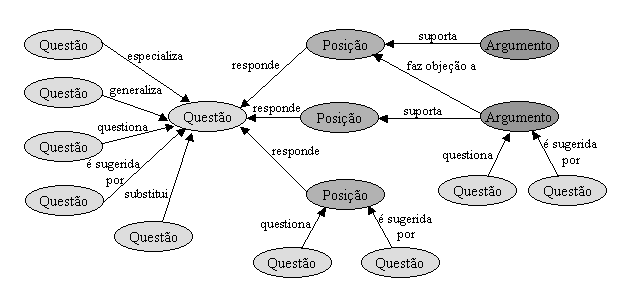
\includegraphics [width=13cm, height=8cm]{fIBIS.png}
  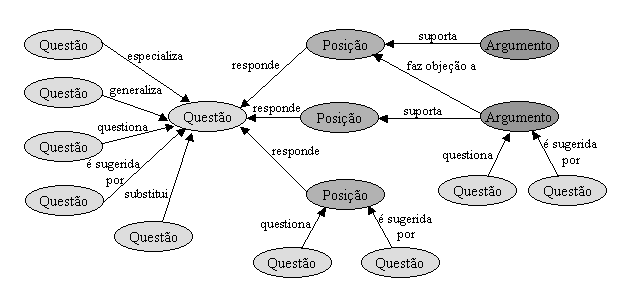
\includegraphics [width=0.75\textwidth]{fIBIS.png}
  \caption {Abstra��es e relacionamentos do modelo IBIS \citep{KunRit70}}
  \label{ibis}
\end{figure}


O modelo PHI estende o modelo IBIS ampliando o escopo do conceito quest�o e alterando a
estrutura que relaciona os seus tipos de n�s. O modelo considera a
hierarquia entre as estruturas e representa as informa��es
capturadas utilizando, al�m das abstra��es de quest�o, resposta e
argumento advindas do IBIS, as abstra��es de sub-quest�o,
sub-resposta e sub-argumento, que indicam um n�vel a mais na
estrutura do modelo, conforme apresentado na Figura \ref{phi}. As rela��es entre os n�s s�o simplificadas
por meio do uso de somente uma rela��o denominada {\it serve}. A
rela��o {\it serve} � definida da seguinte forma: A {\it quest�o A}
serve a {\it quest�o B} se e somente se a resolu��o da {\it
quest�o A} influenciar a resolu��o da {\it quest�o B}. As
abstra��es sub-resposta e sub-argumento s�o definidas de forma
an�loga.

\begin{figure} [!ht]
 \centering
  \bfseries
%  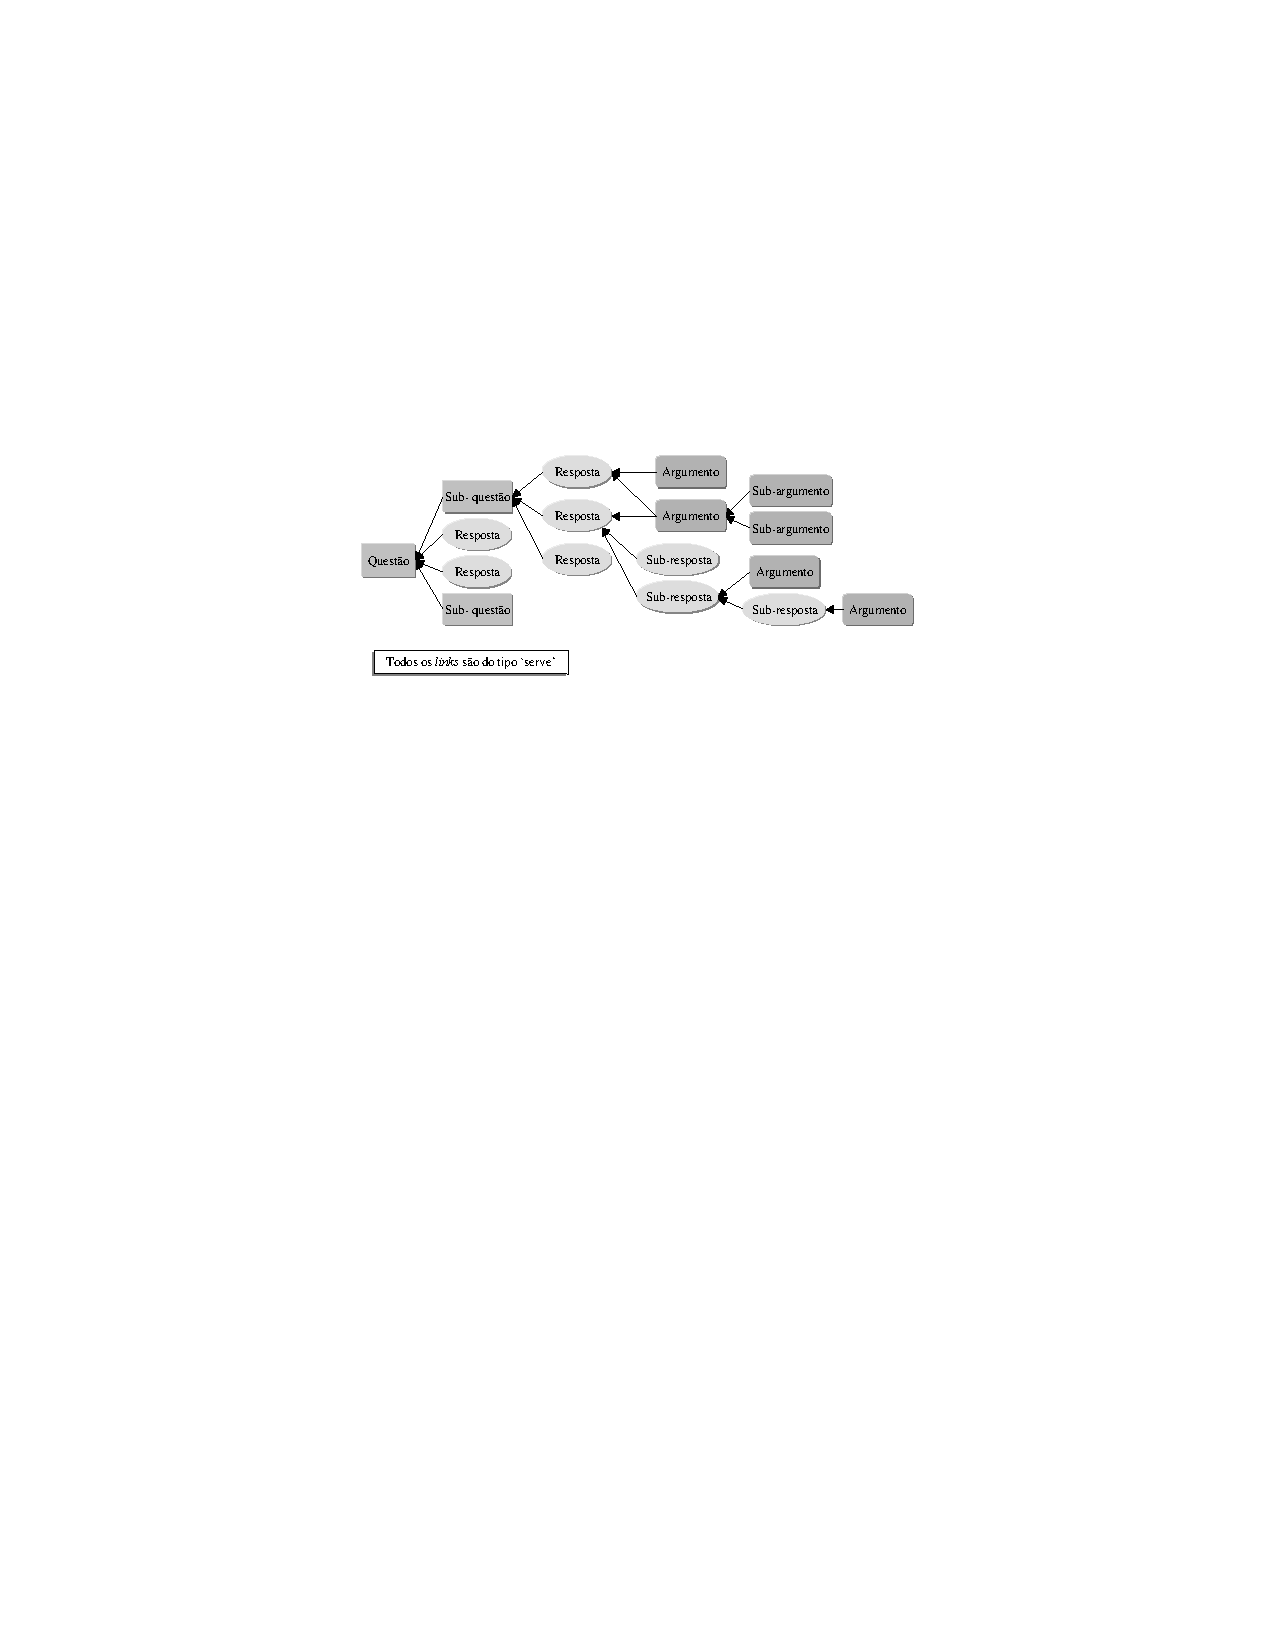
\includegraphics [width=13cm, height=8cm]{fPHI2.pdf}
  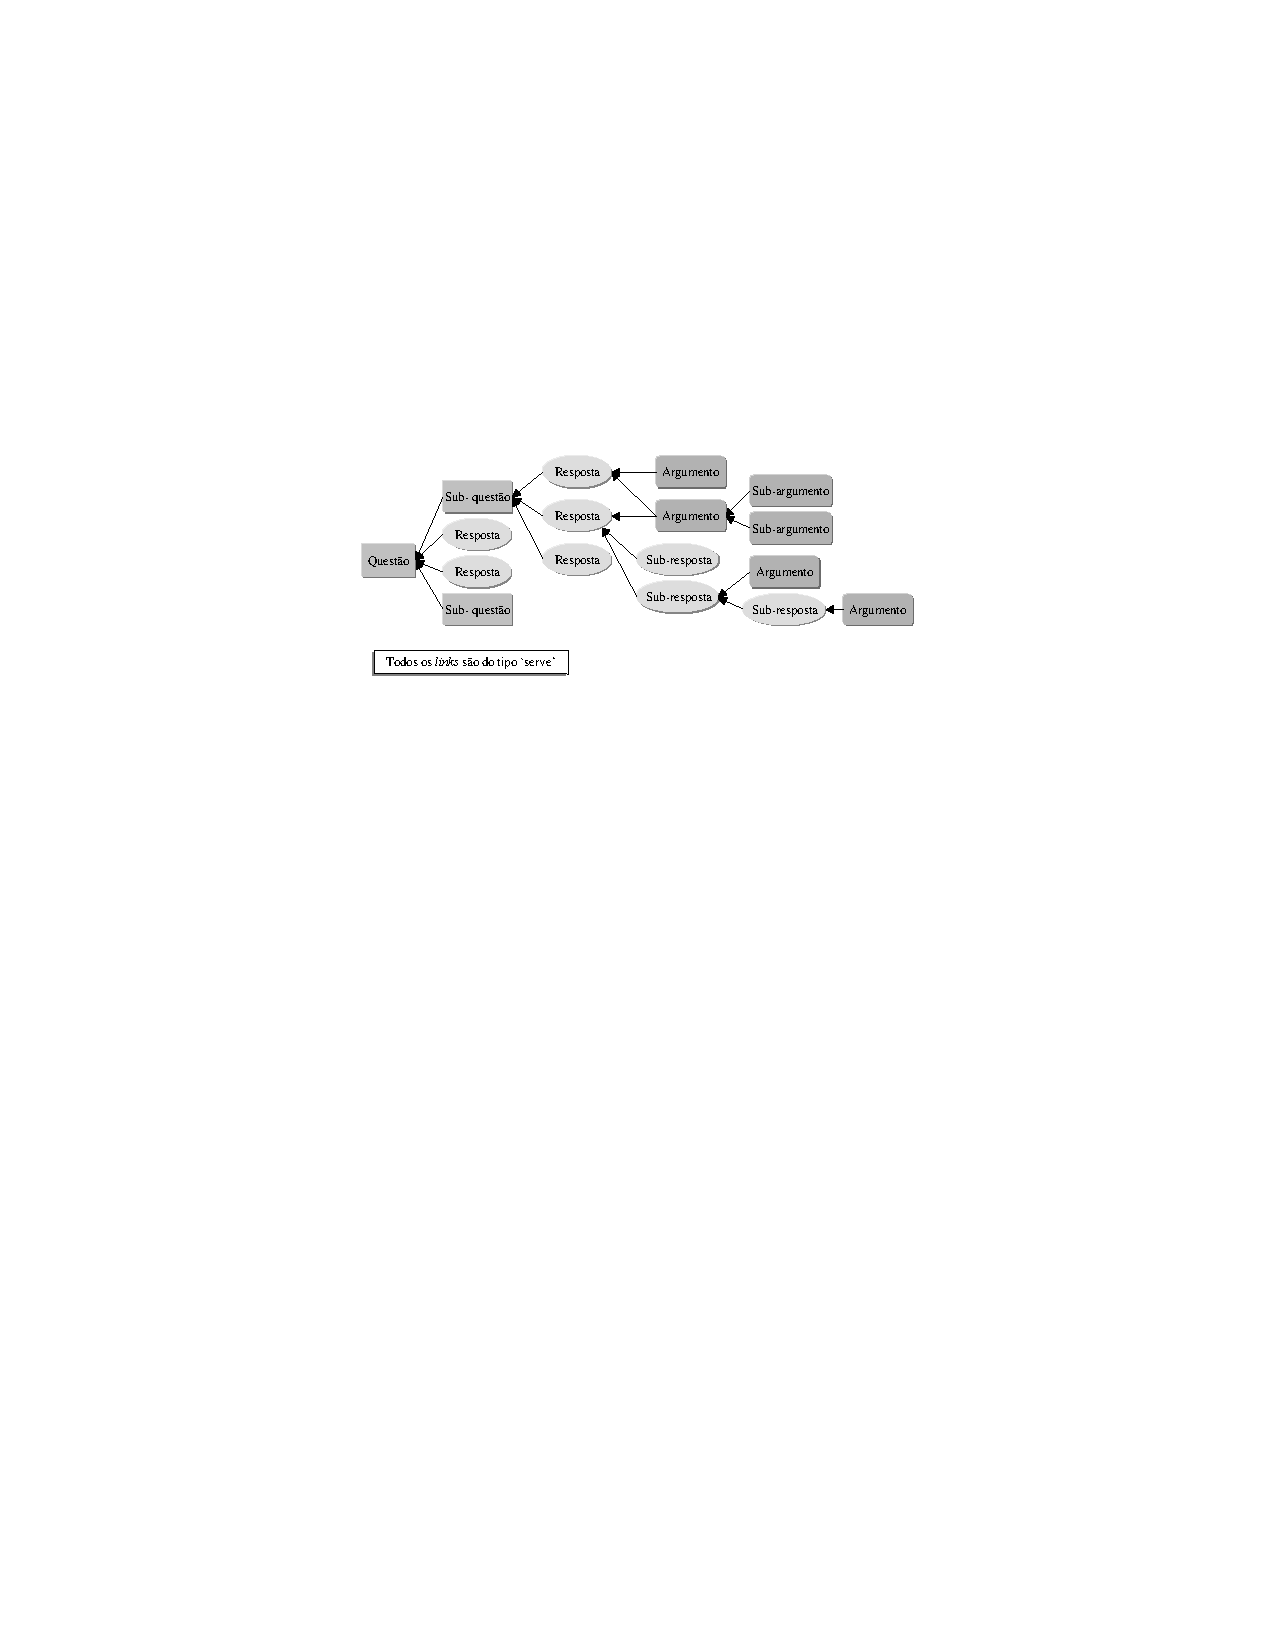
\includegraphics [width=0.80\textwidth]{fPHI2.pdf}
  \caption {Abstra��es e relacionamentos do modelo PHI \citep{McCall91}}
  \label{phi}
\end{figure}

%Outra caracter�stica do modelo PHI � que as quest�es,
%sub-quest�es, respostas, sub-res\-pos\-tas, argumentos e
%sub-argumentos podem ser apresentados em formato linear
%\cite{RegHuAtwSun00}. Obviamente, no caso em que um argumento, por
%exemplo, servir para mais de uma resposta, no formato linear ele
%dever� ser repetido, assim como toda sub-rede que lhe estiver
%associado.

De acordo com \cite{Lu1999}, embora a estrutura hier�rquica aumente a expressividade de PHI, algumas rela��es
importantes ainda n�o podem ser facilmente expressadas, tais como
os crit�rios e objetivos de um projeto.

QOC (\textit{Questions, Options, and Criteria}) � uma nota��o semi-formal que representa o espa�o de projeto
usando tr�s componentes. As quest�es identificam as principais
d�vidas que permitam estruturar o espa�o de alternativas, as
op��es fornecem poss�veis respostas �s quest�es e os crit�rios s�o
a base para avaliar e escolher uma das op��es.

Enquanto os sistemas que usam os modelos IBIS e PHI t�m o
prop�sito de capturar o hist�rico das delibera��es, os sistemas
que usam o modelo QOC enfatizam o desenvolvimento sistem�tico de
um espa�o de op��es de projeto estruturado por quest�es
\citep{RegHuAtwSun00}.

Conforme apresentado na Figura \ref{qoc}, os poss�veis
relacionamentos entre os n�s do QOC s�o: uma op��o {\it responde
a} uma quest�o; uma quest�o {\it � conseq��ncia de} uma op��o; um
crit�rio faz uma {\it avalia��o positiva} de uma op��o e um
crit�rio faz uma {\it avalia��o negativa} de uma op��o. Assim que um n� {\it quest�o} � inserido, v�rios n�s {\it op��o}
s�o inseridos de forma a tentar solucionar a quest�o. Para avaliar
se uma {\it op��o} � v�lida, s�o usados os n�s {\it crit�rio}, com o objetivo de avaliar
uma {\it op��o} ou mais. Sendo
assim, tal avalia��o pode ser positiva ou negativa para a {\it op��o}.
Uma mesma {\it op��o} pode ter um determinado crit�rio a seu favor e
outro contra. %Outras quest�es podem ser inseridas se uma op��o trouxer alguma d�vida. Dessa forma, o n� {\it quest�o} � ligado ao n� {\it op��o} que gerou a d�vida.

%De acordo com Regli et al \cite{RegHuAtwSun00}, o modelo QOC possui vantagens em rela��o ao aspecto de reuso: �
%relativamente f�cil para o desenvolvedor utilizar o QOC para
%produzir {\it design rationale} durante a atividade de engenharia reversa de um
%sistema (ou parte dele). A comunica��o da equipe de projeto �
%armazenada enfatizando as alternativas que foram consideradas,
%quais delas foram escolhidas e porqu�.

\begin{figure} [!ht]
 \centering
  \bfseries
%  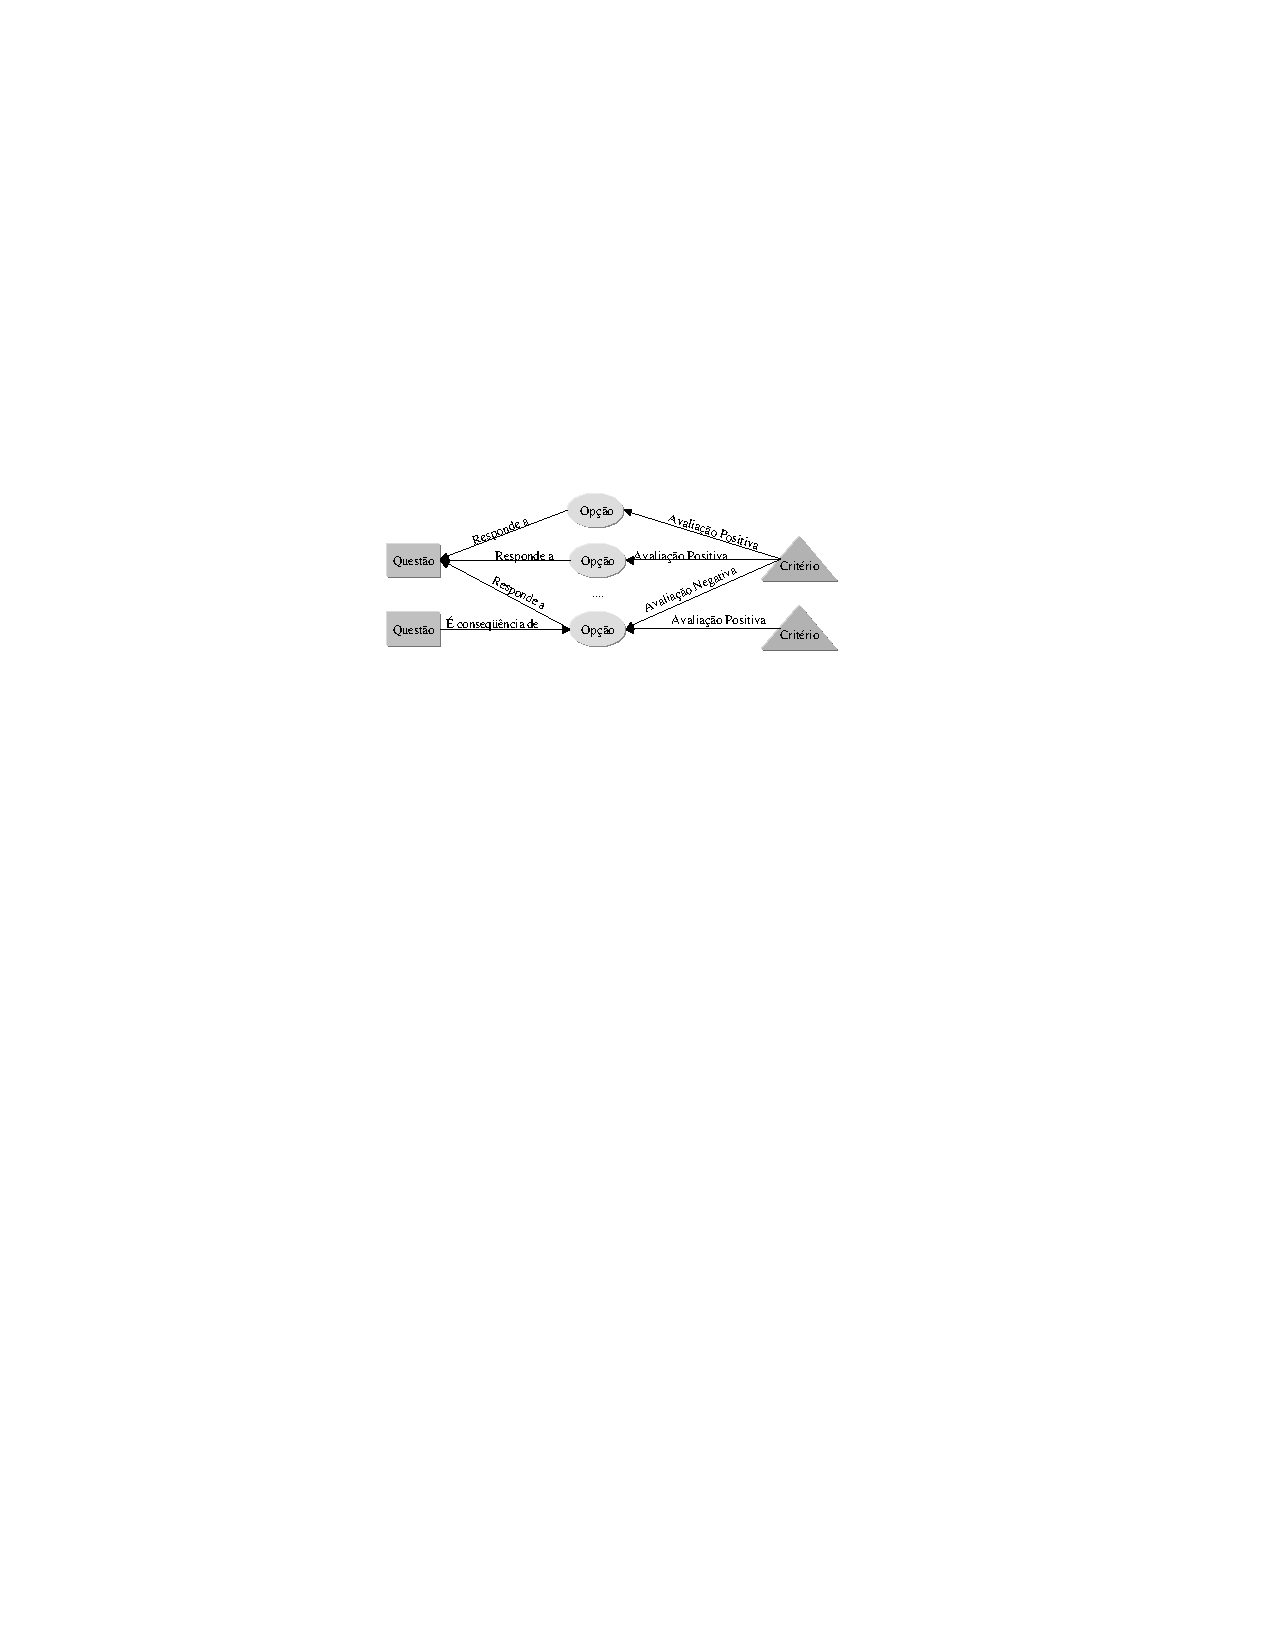
\includegraphics [width=10cm, height=6cm]{fQOC.pdf}
  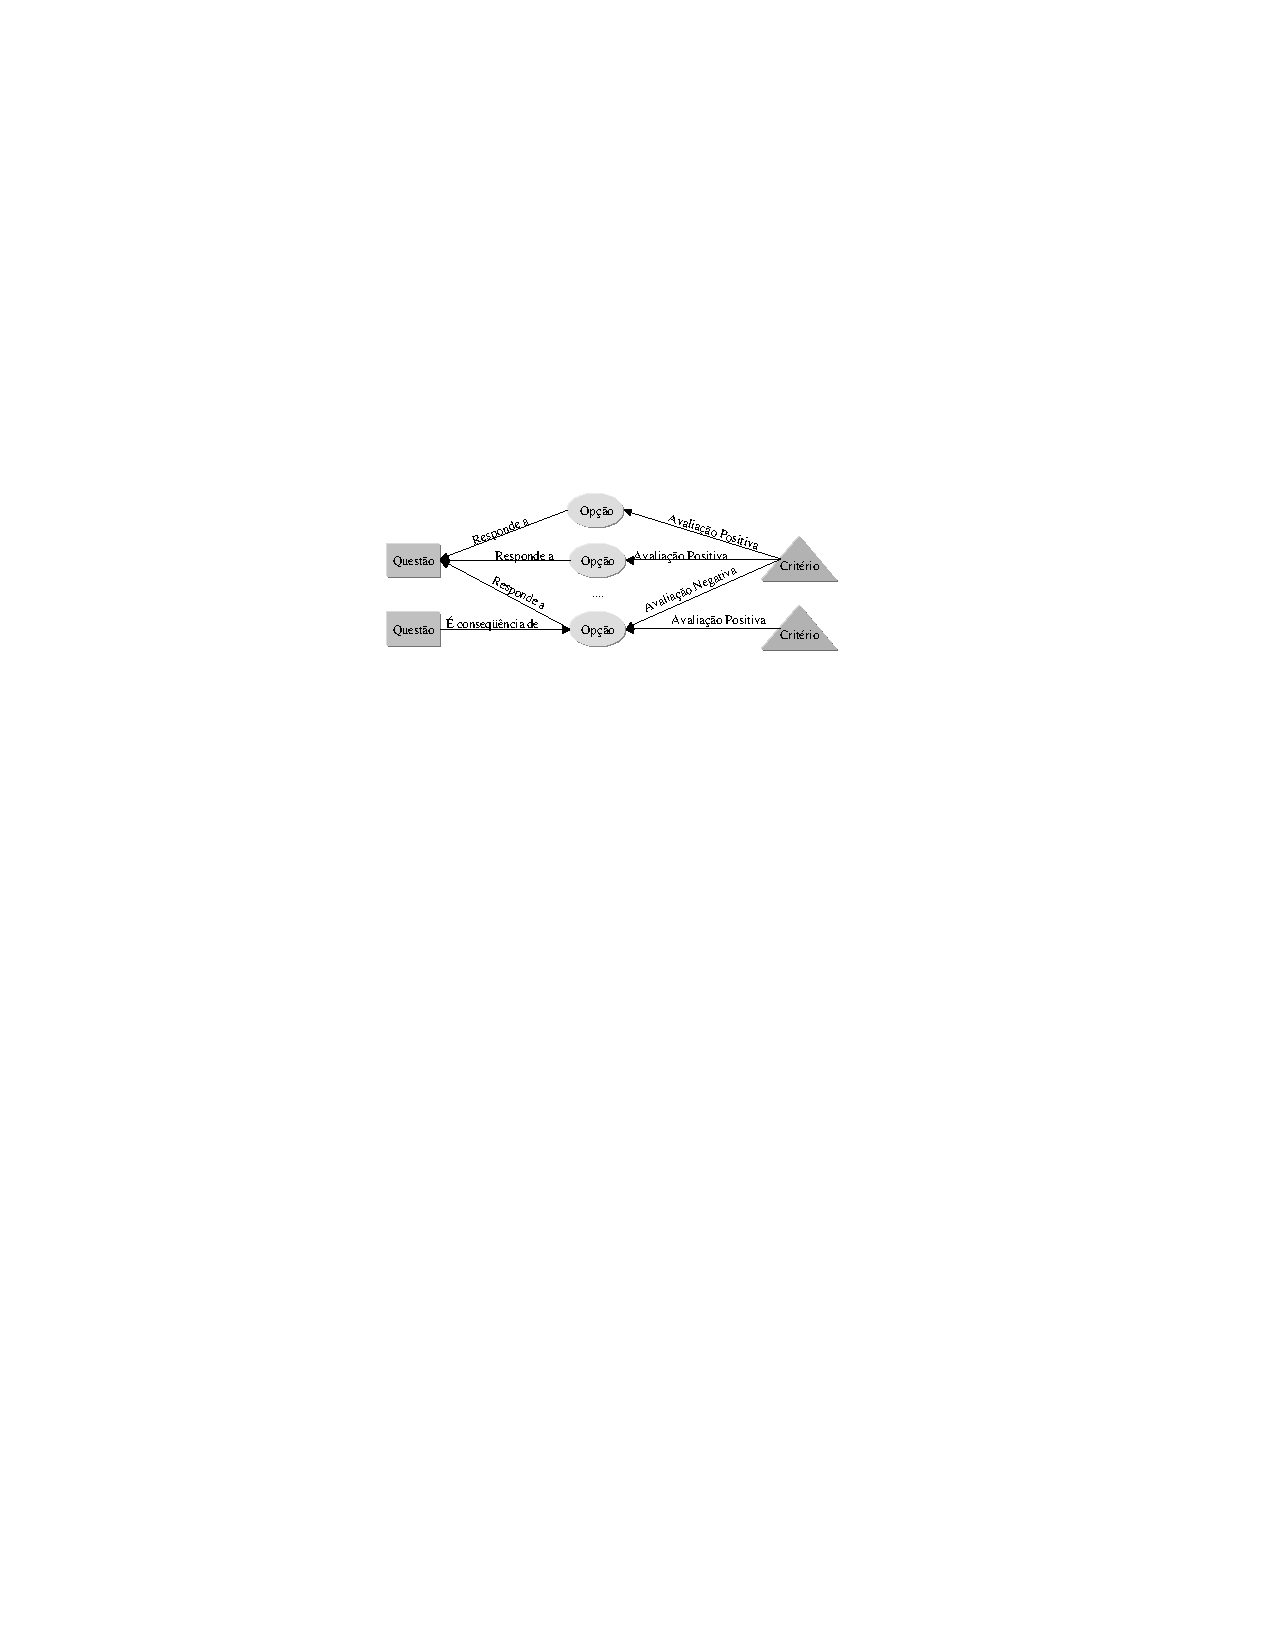
\includegraphics [width=0.70\textwidth]{fQOC.pdf}
  \caption {Abstra��es e relacionamentos do modelo QOC \citep{MacYouBelMor91}}
  \label{qoc}
\end{figure}

%O modelo DRL (\textit{Decision Rationale Language}) � uma extens�o do modelo IBIS, envolvendo um n�mero maior de abstra��es e relacionamentos. Pode ser visto como uma melhoria � extens�o que PHI prop�e sobre o modelo IBIS pela generaliza��o da estrutura hier�rquica em rela��es mais complexas \citep{Bacelo1996}. De acordo com \cite{Lu1999}, o modelo DRL � mais expressivo para a representa��o da decis�o do projeto pois seus objetos capturam v�rios relacionamentos entre os elementos de decis�o.

%O modelo DRL � composto pelos seguintes componentes: problema de decis�o (representa o problema da escolha da alternativa que melhor satisfaz o objetivo), objetivo (propriedades que uma op��o ideal deve ter), alternativa (poss�veis solu��es), alega��o (argumentos a favor ou contra um objetivo ou uma outra alega��o), quest�o (d�vidas/perguntas), procedimento (poss�veis solu��es) e grupo (conjunto de poss�veis solu��es).

%Os poss�veis relacionamentos entre os n�s do DRL s�o: um problema de decis�o {\it � uma sub-decis�o de} outro problema de decis�o; um objetivo {\it � um sub-objetivo de} um problema de decis�o ou outro objetivo; uma alternativa {\it atinge} um objetivo; uma alternativa {\it � uma alternativa para} um problema de decis�o; uma alega��o {\it suporta} uma alternativa ou outra alega��o; uma alega��o {\it � contra} uma alternativa ou outra alega��o; uma alega��o {\it pressup�e} outra alega��o; uma alega��o {\it responde} uma quest�o; uma alega��o {\it � um resultado de} um procedimento; uma alega��o {\it � um membro de} um grupo; uma quest�o {\it questiona} ou {\it influencia} uma alega��o; um procedimento {\it � uma resposta para} uma quest�o; um procedimento {\it � um subprocedimento de} um procedimento; um grupo {\it � um conjunto de poss�veis respostas para} uma quest�o. Uma vis�o geral do modelo DRL � apresentada na Figura \ref{drl}.

%A argumenta��o do DRL inicia com o problema de decis�o. A partir deste problema, um n�mero de sub-objetivos pode ser definido para resolv�-lo e alternativas para tais objetivos s�o determinadas \cite{Monk1995}. Para essas alternativas, surgem alega��es a favor ou contra e, para as alega��es, surgem as quest�es ou outras alega��es.

%\begin{figure} [!ht]
% \centering
%  \bfseries
  %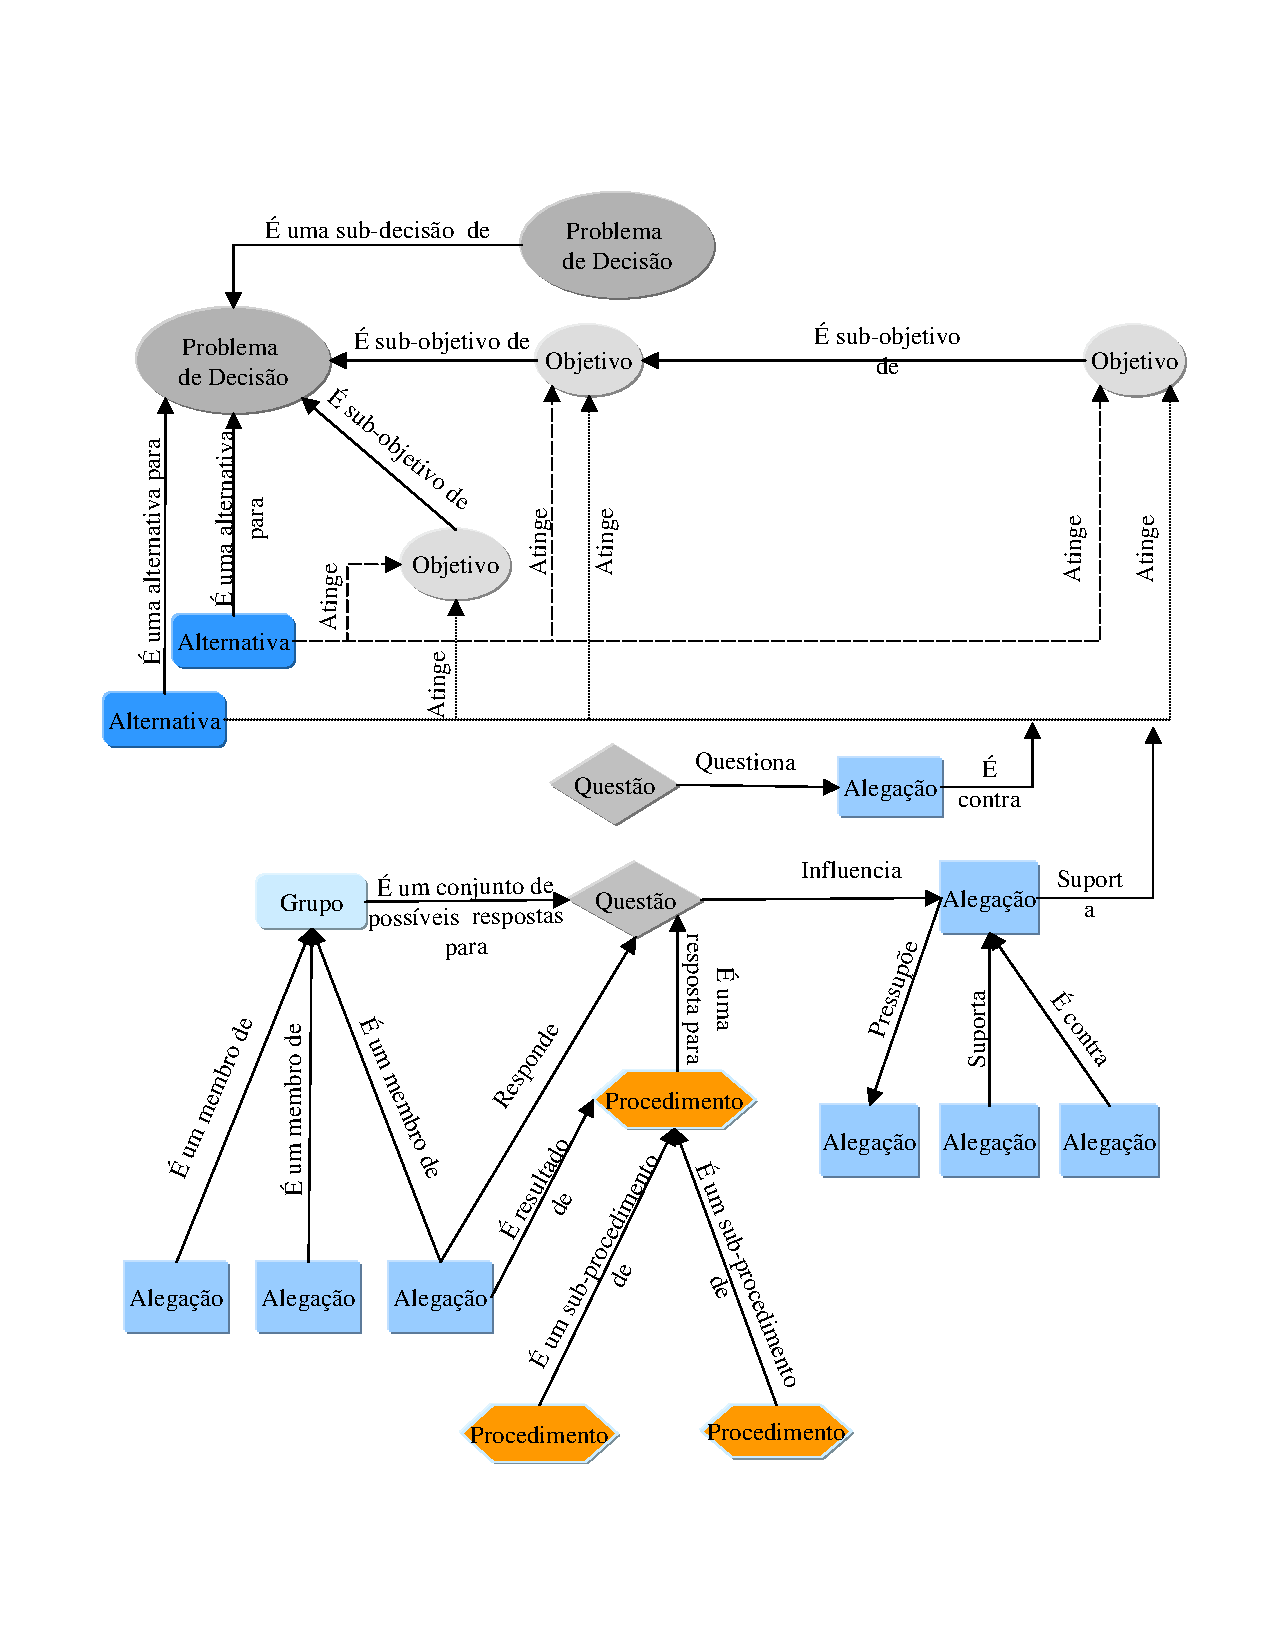
\includegraphics [width=13cm, height=11cm]{fDRL.pdf}
%  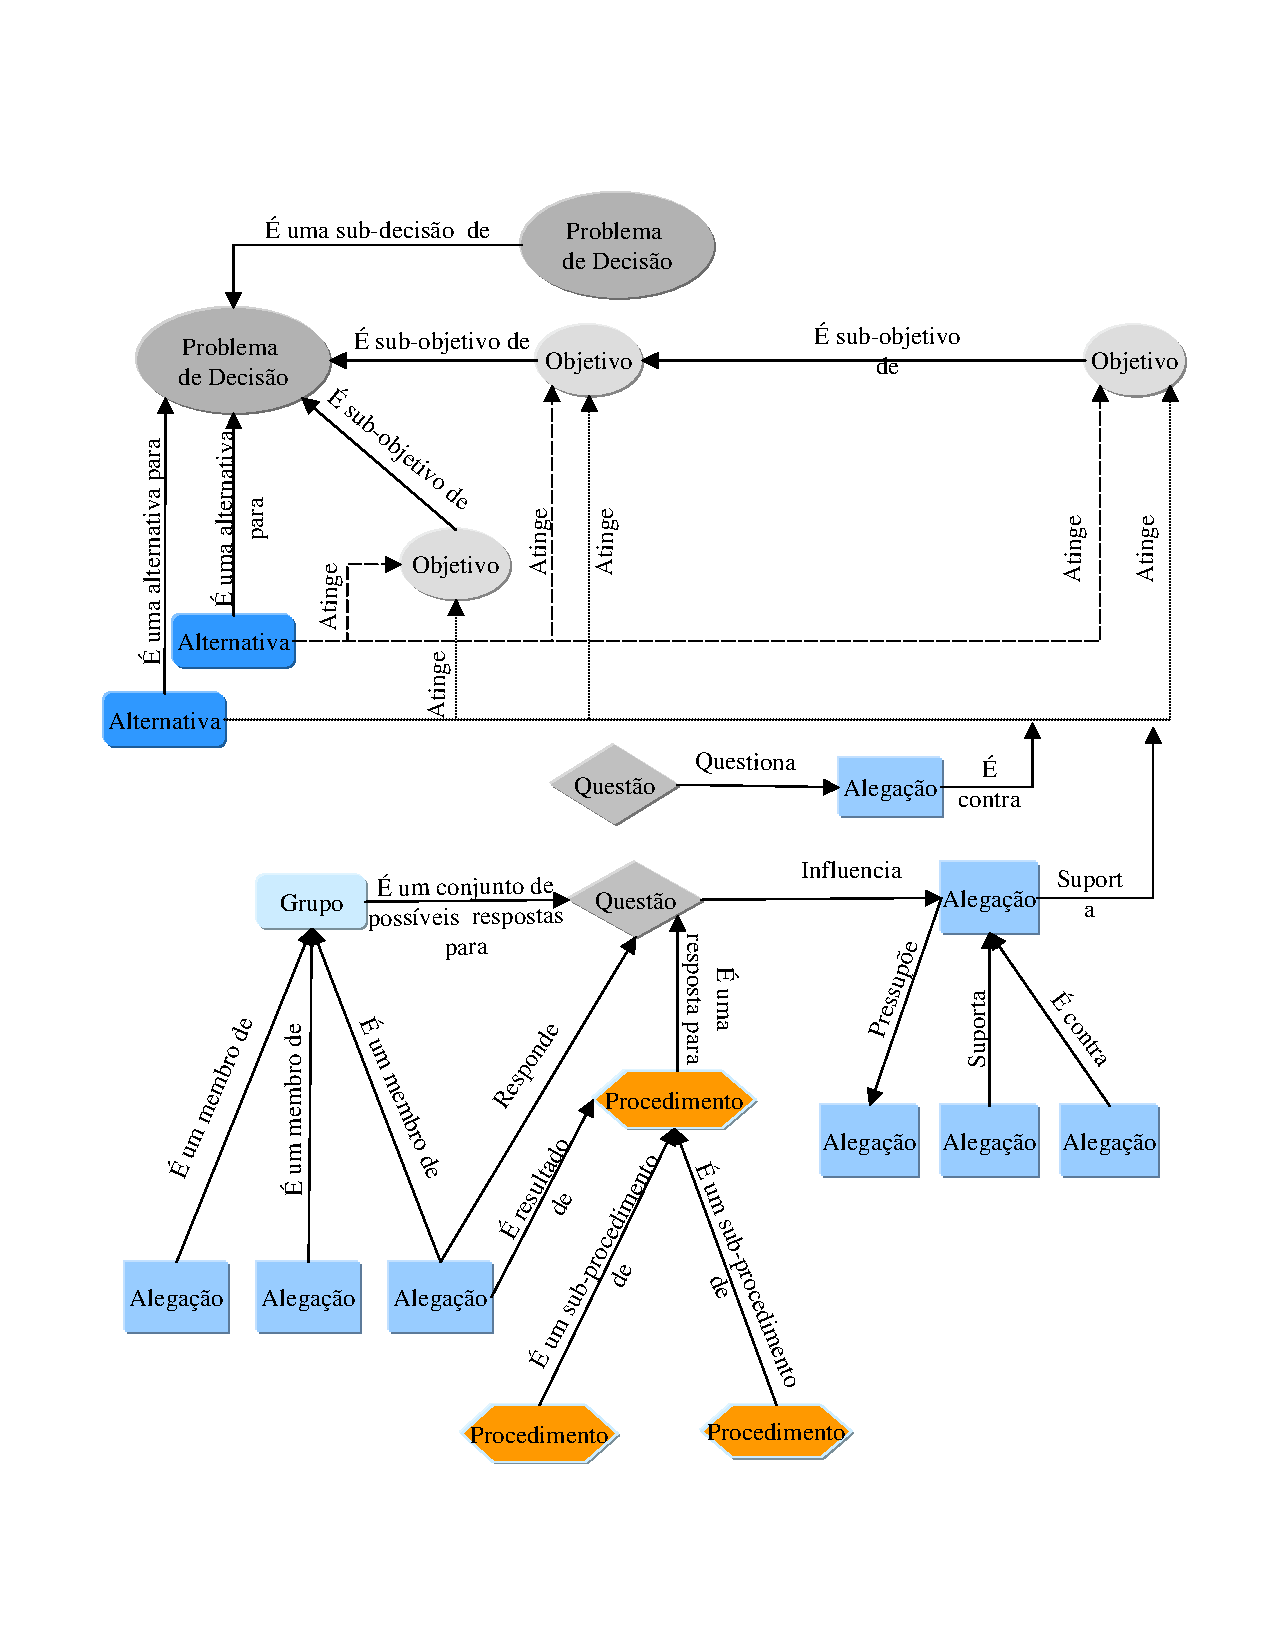
\includegraphics [width=0.75\textwidth]{fDRL.pdf}
%  \caption {Abstra��es e Relacionamentos do Modelo DRL \citep{LeeLai91}}
%  \label{drl}
%\end{figure}

%De acordo com \cite{Wiegeraad1999}, por oferecer um maior n�mero de n�s e de \textit{links}, o modelo DRL facilita a compreens�o da discuss�o que ocorreu entre os membros de um projeto porque a informa��o � representada explicitamente em cada n�, de acordo com a sem�ntica da informa��o. Entretanto, esse grande n�mero de tipos de n�s e \textit{links} exige, durante o armazenamento, cuidados para a correta delimita��o da informa��o correspondente a cada tipo de n� dispon�vel.

Conforme apresentado por \cite{Lee1997}, a representa��o de {\it design rationale} pode ser
informal, semi-formal ou formal. A escolha de uma determinada
abordagem depende dos servi�os que o sistema dever� fornecer. Na representa��o informal, {\it design rationale} � capturado de uma forma n�o estruturada: s�o capturadas descri��es em linguagem natural, registros de �udio e v�deo e
rascunhos de diagramas. Geralmente s�o f�ceis de criar, mas os
sistemas computacionais n�o podem interpret�-los.

Em uma representa��o semi-formal, apenas partes do conte�do pode
ser interpretada computacionalmente. No entanto, os sistemas que
implementam este tipo de representa��o podem suportar muitos
servi�os computacionais cujas implementa��es n�o s�o poss�veis de
implementar quando a representa��o informal � utilizada. Al�m
disso, h� menos sobrecarga aos projetistas na atividade de captura
de {\it design rationale} porque o sistema pode sugerir quais informa��es s�o
esperadas.

Em uma representa��o formal, objetos e rela��es s�o definidos como
objetos formais que o sistema pode interpretar e manipular usando
opera��es formais. A captura de {\it design rationale} torna-se uma forma de criar uma
base de conhecimentos utilizando-se uma linguagem formal.
Observa-se, ainda, que quanto mais formalmente representadas
estiverem as informa��es de {\it design rationale}, mais servi�os o sistema poder� fornecer automaticamente. O autor
sugere a utiliza��o de uma abordagem incremental como forma de
minimizar o custo da formaliza��o do conhecimento, ou seja,
transformando uma representa��o semi-formal em uma representa��o
formal. %Dessa forma, as informa��es de {\it design rationale} podem ser capturadas com menos sobrecarga
%(porque eles s�o capturados utilizando uma representa��o
%semi-formal) e, uma vez formalizados, podem ser usados para
%suportar diversos servi�os computacionais.

Conforme observado por \cite{Wiegeraad1999}, os modelos
apresentados compartilham as mesmas estruturas b�sicas de
``problema de projeto'', ``solu��o alternativa'', ``argumentos'' e
``crit�rios'', ou seja, diferentes termos s�o usados para
representar basicamente os mesmos conceitos. Nota-se, tamb�m,
que os modelos de representa��o s�o bastante gen�ricos, o que sugere a possibilidade de uma extens�o ou adapta��o dos mesmos de acordo com as peculiaridades do dom�nio de aplica��o.

Ressalta-se o fato de que as pesquisas tendem a usar a perspectiva de argumenta��o e o modelo IBIS para a representa��o de {\it design rationale}. Possivelmente isto ocorre devido ao fato de ser o modelo mais gen�rico e que fornece uma estrutura b�sica que pode ser adaptada para outros ambientes.

Um elemento importante em rela��o ao desenvolvimento de projetos de pesquisa � a express�o da {\it criatividade}. Em geral, h� poucos resultados indicando a rela��o entre o uso de abordagens de {\it design rationale} e a explora��o da criatividade. O �nico registro encontrado se refere ao trabalho de \cite{ngu06}. Os autores propuseram a integra��o dos modelos IBIS e QOC � atividade de engenharia de requisitos. Al�m disso, eles sugeriram o uso do modelo IBIS durante a execu��o de atividades de an�lise e modelagem de requisitos, em que s�o realizadas, por exemplo, sess�es de {\it brainstorming} e reuni�es para discuss�o e entendimento geral do projeto. Foi proposta uma modifica��o no modelo acrescentando um elemento {\it contexto} a cada {\it quest�o} registrada, com o objetivo de indicar a situa��o espec�fica em que foram geradas. Al�m disso, os autores sugeriram o uso do modelo QOC para a descri��o do ``espa�o do problema'', de forma a auxiliar o entendimento do ambiente para o qual o sistema est� sendo desenvolvido. A rela��o entre a express�o da criatividade e o uso dos modelos IBIS e QOC � apresentada, principalmente, da seguinte forma: %\footnote{N�o foram apresentados resultados experimentais que pudessem comprovar a rela��o entre a express�o da criatividade e o uso dos modelos.}:

\begin{itemize}

\item O modelo IBIS incentiva a discuss�o de id�ias e, consequentemente, contribui para que as d�vidas dos desenvolvedores e dos usu�rios se tornem mais claras e sejam conhecidas. Outro fator importante � que o modelo IBIS suporta a comunica��o entre engenheiros de requisitos ao possibilitar que quest�es e poss�veis solu��es sejam compartilhadas e debatidas\footnote{Os autores n�o apresentaram caracter�sticas espec�ficas do modelo IBIS que tenham motivado sua ado��o. Portanto, surge a d�vida sobre a aplicabilidade de outros modelos no contexto do trabalho apresentado};

\item O modelo QOC � �til por ajudar o engenheiro de requisitos a examinar o ``espa�o do problema'' em pontos cr�ticos durante a atividade de engenharia de requisitos, a reconhecer e avaliar {\it insights}, a avaliar o espa�o do problema e a re-estruturar o modelo de requisitos.

\end{itemize}

\subsection{Recupera��o de {\it design rationale}}

A recupera��o de {\it design rationale} � determinada, principalmente, pelo esquema de representa��o
utilizado. Algumas situa��es (cen�rios)
que motivam a recupera��o de {\it design rationale} se referem � visualiza��o de
projetos similares e suas decis�es associadas; � recupera��o de
crit�rios, regras e op��es que ajudem a tomar decis�es durante o
projeto e � produ��o de documentos ap�s o processo de projeto
\citep{RegHuAtwSun00}.

Diferentes estrat�gias de recupera��o podem ser utilizadas,
dependendo dos interesses dos usu�rios do sistema.
\cite{RegHuAtwSun00} consideram tr�s poss�veis abordagens: navega��o, pesquisa ou recupera��o autom�tica.
Na abordagem da {\it navega��o}, os projetistas podem verificar o {\it design rationale},
percorrendo {\it n�s} por meio de \textit{links} existentes entre
eles. Para o projeto de um artefato complexo, geralmente uma
grande quantidade de informa��o � armazenada, o que dificulta a
busca por respostas espec�ficas utilizando a
estrat�gia de navega��o. A recupera��o por {\it pesquisa} � considerada
mais eficiente que a recupera��o com base em navega��o. As
consultas podem seguir a estrutura ``o que acontece se'' ({\it
what-if}), que podem ser respondidas explorando-se diferentes
op��es; ou a estrutura ``por que'', que s�o respondidas fazendo-se
{\it backtracking} na rede de n�s e \textit{links} com a
finalidade de encontrar a argumenta��o ou o racioc�nio
relacionado � decis�o. Na recupera��o {\it autom�tica}, � feito um
monitoramento do desenvolvimento de um projeto, de acordo com as
regras, os crit�rios e as restri��es definidas. Um monitor �
utilizado para observar e verificar o processo de projeto e
comparar as decis�es tomadas com regras, crit�rios e restri��es da
biblioteca de {\it design rationale} ou da base de conhecimento. Quando s�o
encontradas diferen�as, o {\it design rationale} � apresentado automaticamente.

Em rela��o � recupera��o de {\it design rationale}, os sistemas s�o classificados por \cite {Lee1997} como sistemas de iniciativa do usu�rio ou de
iniciativa do pr�prio sistema. No primeiro caso, o usu�rio decide
quais partes do {\it design rationale} ser�o examinadas, quando e como ser�o
visualizadas. Estes sistemas devem auxiliar os usu�rios a tomar
conhecimento das informa��es armazenadas e tornar f�cil o acesso
�s partes desejadas. No segundo caso, o sistema utiliza uma base
de conhecimentos para decidir quando e como apresentar um {\it design rationale} (ou
partes dele). Tais sistemas devem possuir uma base de
conhecimentos que possa auxiliar efetivamente o sistema a tomar
decis�es e devem ser capazes de apresentar as informa��es de {\it design rationale} de forma n�o
intrusiva.

\cite{ChuGoo1998} propuseram o sistema IDIS ({\it
Integrated Design Information System}), que apresenta o projeto de
um determinado sistema e as anota��es relacionadas �s entidades do
projeto. Quando um projetista clica em um item de um diagrama, a
especifica��o desse item � apresentada bem como todas as quest�es
e coment�rios relacionados a ele. O sistema permite tamb�m que o
projetista possa acompanhar o progresso do projeto e revisar todas
as etapas cumpridas. Os usu�rios podem tratar o sistema como uma
base de texto, de forma que possa ser realizada uma busca por
palavras-chave para determinar o que foi discutido sobre um
determinado t�pico. Al�m disso, para responder quest�es
relacionadas a ``como atingimos determinado est�gio'', o sistema
apresenta todas as informa��es relevantes que influenciaram a
escolha de uma alternativa particular de projeto. Para responder
quest�es relacionadas a diferen�as entre duas alternativas de
projeto, o sistema fornece um resumo das discuss�es que levaram a
diferentes alternativas de projeto, dados que fazem parte de um
projeto e n�o fazem parte de outro e valores diferentes de
par�metros associados aos mesmos itens em diferentes projetos.

\cite{BurBro2002} observaram que grande parte das pesquisas
atuais focaliza a captura e a representa��o de {\it design rationale}. Os autores acreditam
que estas atividades s�o muito importantes, por�m o sucesso das mesmas
est� relacionado � utilidade de {\it design rationale} para projetos em
desenvolvimento, ou seja, o valor real de um {\it design rationale} s� pode ser
avaliado quando ele de fato for �til em um projeto. Capturar
grande quantidade de informa��es detalhadas n�o � relevante se
tais informa��es n�o forem acessadas. Por outro lado, se o {\it design rationale} �
�til no desenvolvimento dos projetos da organiza��o, h� um maior
incentivo para que o projetista se empenhe na captura das
informa��es necess�rias, particularmente se elas puderem ser
utilizadas imediatamente. Al�m disso, conhecendo-se como as
informa��es ser�o utilizadas, � poss�vel determinar o que
deve ser capturado e como o conte�do obtido deve ser representado.

 Na se��o seguinte � enfatizado, portanto, o uso de {\it design rationale}, observando-se como os principais conceitos est�o sendo aplicados na pr�tica e os benef�cios que a abordagem pode trazer para o ambiente de desenvolvimento de projetos de pesquisa.

%Karsenty \cite{Kar96} realizou estudos emp�ricos com o objetivo de analisar a utilidade de documentos de DR. Foi solicitado que seis projetistas experientes tentassem
%compreender e avaliar projetos passados para os quais os DRs
%estavam dispon�veis e podiam ser consultados. O autor concluiu que os documentos de DR foram �teis para os projetistas que os acessaram para ajudar no racioc�nio do projeto. No entanto, n�o foram suficientes para responder a todas as perguntas dos projetistas.


\section{Uso de {\it design rationale}}

De acordo com \cite{dut06}, {\it design rationale} pode ser utilizado principalmente com os seguintes prop�sitos: 

\begin{itemize} 
\item promover a colabora��o entre membros de uma equipe, 
\item facilitar a manuten��o e o reuso,
\item  melhorar a qualidade dos artefatos e 
\item transferir conhecimentos. 
\end{itemize}

A seguir, s�o apresentados trabalhos de pesquisa que est�o sendo realizados no sentido de explorar as potencialidades de {\it design rationale} em rela��o aos seus prop�sitos.

%Nesse sentido, um dos objetivos deste trabalho foi observar como a abordagem de {\it design rationale} poderia contribuir na proposta de um processo para o desenvolvimento de projetos de pesquisa, considerando-se que os objetivos do processo est�o diretamente relacionados aos prop�sitos mencionados pelo autor. A seguir s�o apresentados os coment�rios do autor sobre o uso de {\it design rationale} e resultados de pesquisa que est�o sendo obtidos.

\subsection{Visando colabora��o}

Membros de uma equipe podem usar um reposit�rio de {\it design rationale} para compreender as atividades que os outros membros est�o cumprindo e como estas atividades podem impactar em seus pr�prios trabalhos. Outra possibilidade de uso � a exposi��o de diferentes pontos de vista e o racioc�nio associado. Al�m disso, {\it design rationale} � importante para promover o projeto participativo e colaborativo, de forma que os usu�rios possam compreender o racioc�nio dos projetistas, as quest�es que est�o sendo tratadas pelos desenvolvedores e as alternativas que est�o sendo consideradas \citep{dut06}.

\cite{fal06} propuseram uma t�cnica para documentar raz�es das decis�es de projeto ({\it design decision rationale}) e avaliaram experimentalmente seu impacto em rela��o � efic�cia e efici�ncia quando membros de diferentes equipes que desenvolvem um projeto precisam colaborar para que uma decis�o seja tomada quando h� mudan�as de requisitos. Os autores propuseram uma t�cnica de documenta��o denominada DGA ({\it Decision Goals and Alternatives}), que considera que as decis�es de projeto dependem dos objetivos da decis�o e de relacionamentos entre decis�es. De forma geral, eles sugeriram que as seguintes informa��es sejam capturadas: requisitos funcionais, requisitos n�o funcionais (atributos de qualidade e restri��es), objetivos de neg�cios e decis�o.

Na abordagem proposta, o conceito {\it decis�o} � refinado em dois sub-conceitos: tipo de decis�o (DT) e alternativas de decis�o (DA). DT se refere ao problema que a decis�o deve solucionar e DA representa as alternativas dispon�veis. Os autores realizaram experimentos com a abordagem proposta para avaliar os efeitos da abordagem em situa��es em que indiv�duos e equipes precisavam tomar decis�es. Para ambos os casos, os resultados obtidos indicaram que a efic�cia melhorou quando a documenta��o segundo o formato DGA est� dispon�vel e a efici�ncia permaneceu inalterada.

\subsection{Visando manuten��o e reuso}

Em geral, pesquisadores entendem que um dos principais usos para {\it design rationale} est� associado ao cumprimento da atividade de manuten��o. Pessoas respons�veis por fazer altera��es precisam compreender os efeitos das mudan�as, bem como as raz�es pelas quais os artefatos foram elaborados daquela determinada forma, e o conhecimento das raz�es de projeto ajudam nessa compreens�o. De forma semelhante, antes que o software possa ser reusado � necess�rio que seja entendido e/ou modificado. Isso requer que o racioc�nio dos desenvolvedores do projeto seja entendido e que os componentes, elementos ou m�dulos que podem ser reusados sejam identificados \citep{dut06}.
Em um estudo realizado recentemente, \cite{bab06} observaram que, na pr�tica, projetistas e desenvolvedores do setor industrial percebem a utilidade de {\it design rationale} e percebem tamb�m que os esfor�os dispendidos na captura das informa��es, tendo em vista os benef�cios que podem ser obtidos na fase de manuten��o, valem a pena.

\cite{lou93} propuseram um sistema de documenta��o cujo objetivo � fornecer apoio a grupos de pessoas que cumprem atividades de manuten��o de software. Para o desenvolvimento do sistema foi explorada a tecnologia de hipertextos juntamente com um mecanismo de anota��o flex�vel, de forma que informa��es de manuten��o sejam registradas em uma ``mem�ria'' do projeto. As informa��es de {\it design rationale} relativas � manuten��o s�o associadas � parte espec�fica do sistema que est� sendo mantida (por exemplo, adicionando coment�rios ao c�digo fonte), podendo ser facilmente visualizadas e alteradas por outras pessoas envolvidas com o projeto. Os autores n�o fizeram restri��es em rela��o � representa��o da informa��o. Como aspecto positivo desse trabalho, pode-se destacar a facilidade de uso: os mantenedores podem incluir as informa��es em um formato livre, e n�o precisam se preocupar em apresent�-la de acordo com as categorias dispon�veis. %De acordo com X, esse � um mecanismo que facilita a captura do conhecimento t�cito, que � o tipo de conhecimento mais dif�cil de obter (???).
Por outro lado, a abordagem utilizada pelos autores dificulta a recupera��o de informa��es espec�ficas.

%Loughere e Rodden argumentaram que as informa��es de {\it design rationale} capturadas durante a fase de manuten��o s�o diferentes daquelas capturadas durante o desenvolvimento. Os autores buscaram uma alternativa � argumenta��o. A abordagem utilizada por eles (...).

\cite{burlivro} t�m investigado como {\it design rationale} pode ser �til para auxiliar a manuten��o de software. Foi proposto o modelo RATSpeak, baseado no modelo de argumenta��o DRL, para a representa��o do {\it design rationale}. Al�m disso, foi desenvolvida a ferramenta SEURAT ({\it Software Engineering Using Rationale}) com o objetivo de oferecer suporte automatizado ao uso de {\it design rationale} na fase de manuten��o, utilizando o modelo RATSpeak. A ferramenta apresenta as informa��es de {\it design rationale} ao mantenedor e faz infer�ncias para detectar problemas e inconsist�ncias que possam indicar problemas no projeto. A ferramenta foi proposta como um {\it plug-in} do sistema Eclipse. Buscou-se, com isso, integrar o c�digo com a informa��o de {\it design rationale} e assegurar que os mantenedores estar�o cientes de que as informa��es est�o dispon�veis e podem ser acessadas facilmente.  %Canfora et al tamb�m tratam o uso de {\it design rationale} em manuten��o. Eles consideram que as informa��es capturadas podem ser observadas de duas formas diferentes. Eles tratam do {\it design rationale} gen�rico e espec�fico.

\subsection{Visando a melhoria de qualidade}

O registro de {\it design rationale} auxilia a identifica��o das decis�es tomadas pelas equipes que desenvolvem o projeto e na certifica��o de que as decis�es s�o mutuamente consistentes. A rastreabilidade de requisitos tamb�m pode ser melhorada, pois � poss�vel fazer liga��es entre requisitos e partes de outros artefatos que est�o relacionados a eles. Al�m disso, {\it design rationale} pode ser utilizado para auxiliar a execu��o de atividades como depura��o, corre��o de problemas e extens�o de funcionalidades de um artefato \citep{dut06}.

\cite{Bal05} investigaram a possibilidade de utilizar {\it design rationale} para auxiliar a reengenharia, o reuso e a melhoria de processos de neg�cios. Eles propuseram a captura de informa��es de {\it design rationale} para cada um dos pap�is envolvidos na modelagem de processos de neg�cios. De acordo com os autores, em geral, processos de neg�cios s�o dif�ceis de compreender se n�o houver uma exposi��o clara do {\it design rationale} que justifica a estrutura do processo. Dessa forma, foi proposto um m�todo que sugere aos projetistas de processos de neg�cios que definam explicitamente como as atividades foram agrupadas e como est�o relacionadas na especifica��o do processo. As fases que comp�em o m�todo proposto para a modelagem de processos de neg�cios s�o: 

\begin{enumerate}
\item  definir as atividades que ir�o compor o processo, em que se prop�e que informa��es de {\it design rationale} sejam capturadas utilizando-se modelos tradicionais; 
\item  definir atividades alternativas (para cada alternativa s�o especificadas restri��es, que s�o consideradas partes do {\it design rationale}) e a rela��o de depend�ncia entre todas as atividades que comp�em o modelo e 
\item  escolher a alternativa adequada, na qual um projeto ser� baseado. 
\end{enumerate}

Os autores enfatizam que o m�todo proposto contribui para a captura de {\it design rationale} devido a possibilidade de raciocinar explicitamente em termos de composi��o de atividades de um processo. Adotando o m�todo, � poss�vel explicitar quem � respons�vel por qual atividade e como elas s�o integradas no modelo de processos de neg�cios resultante. Um ponto positivo do trabalho � o fato de tratar {\it design rationale} sob a perspectiva de processos, diferentemente da maioria dos trabalhos, que enfatiza o produto. Outro ponto a ser destacadado � o respaldo ao cumprimento do modelo de processo de neg�cios de forma colaborativa. Os autores sugeriram que, ao cumprir o processo, informa��es relacionadas �s dimens�es {\it o que}, {\it quem}, {\it onde} e {\it quando} sejam registradas. Uma restri��o ao trabalho observada foi a falta de estudos experimentais envolvendo a proposta.


\subsection{Visando a transfer�ncia de conhecimento}

Para aprender a partir de experi�ncias passadas � necess�rio compreender o caminho seguido para tomar decis�es e os benef�cios e os problemas associados a ele. {\it Design rationale} pode ser �til para auxiliar a reutiliza��o de conhecimento, como alternativa para o registro de id�ias e projetos que foram bem sucedidos ou que n�o geraram bom resultado. Outro uso importante para {\it design rationale} � no treinamento de pessoas que passam a compor uma equipe. Um novo membro pode compreender as raz�es para o estado corrente de um artefato antes de sugerir mudan�as \citep{dut06}.

Conforme apresentado por \cite{hag06}, \textit{patterns} est�o relacionados a {\it design rationale} porque buscam capturar o conhecimento que possa ser reutilizado. Os autores apresentaram um mapeamento entre as categorias usadas para descrever um \textit{pattern } e os n�s do modelo QOC. Eles observaram, como principal diferen�a, o fato de que no modelo QOC, todo o conjunto de op��es pode estar contido em um �nico esquema e, em rela��o a \textit{patterns}, somente uma op��o � proposta. O conjunto de solu��es  � apresentado em uma fam�lia de \textit{patterns} tratando o mesmo problema.


%\section{Design Rationale em Engenharia de Software}


%S�o apresentados, a seguir, resultados que t�m sido apresentados na literatura em termos de aplica��o de {\it design rationale} em Engenharia de Software.

%A abordagem SCRAM foi proposta por Sutcliffe com o objetivo de viabilizar a combina��o de v�rias t�cnicas para elicita��o de requisitos e o modelo de representa��o QOC. Ao elicitar os requisitos, s�o apresentadas aos usu�rios informa��es de {\it design rationale}, enfatizando-se vantagens e desvantagens das alternativas e decis�es tomadas anteriormente, em outros projetos. Em outra abordagem \cite{Pot99}, s�o combinados {\it design rationale} e cen�rios durante o processo de elicita��o de requisitos com o objetivo de auxiliar o refinamento e a revis�o dos mesmos. Para auxiliar a checagem (avalia��o) de requisitos, foi proposta a ferramenta C-ReCS \cite{kl93}, em que os usu�rios especificam os requisitos e o sistema faz uma avalia��o em rela��o � completude, consist�ncia e corretude. Caso detecte algum problema, o sistema tenta explicar as causas ao usu�rio, usando uma �rvore de decis�o pr�-definida.

%A abordagem SCRAM foi proposta por Sutcliffe com o objetivo de viabilizar a combina��o de v�rias t�cnicas para elicita��o de requisitos e o modelo de representa��o QOC. Ao elicitar os requisitos, s�o apresentadas aos usu�rios informa��es de {\it design rationale}, enfatizando-se vantagens e desvantagens das alternativas com rela��o a um conjunto de crit�rios identificados anteriormente, em outros projetos. Ao tornar as informa��es expl�citas aos usu�rios, os engenheiros de requisitos podem avaliar as solu��es adotadas e tamb�m adicionar crit�rios. Em geral, a apresenta��o de muitas op��es favore a discuss�o com usu�rios finais e resulta na elicita��o de outros tipos de informa��o.

%O ciclo {\it Inquiry} � um modelo de processo para defini��o de requisitos que inclui tr�s atividades: express�o, discuss�o e compromisso. Na atividade de express�o, os desenvolvedores adquirem conhecimento sobre o dom�nio, identificam os requisitos e os cen�rios. Na atividade de discuss�o os requisitos s�o comentados e anotados e na atividade de compromisso as decis�es em rela��o aos requisitos s�o tomadas. Foi proposta uma ferramenta que oferece suporte para discuss�es de acordo com a estrutura do modelo IBIS.

%Em rela��o � fase de projeto de software, Myers et al \cite{Mye1999} apresentaram um {\it framework} cujo objetivo � promover o registro de informa��es de {\it design rationale} evitando a interrup��o das atividades de projeto. A abordagem envolve a monitoria das intera��es do projetista com uma ferramenta de aux�lio ao projeto (CAD -- {\it Computer-Assisted Design} com o objetivo de gerar dados hist�ricos, que s�o estruturados e interpretados para auxiliar a explica��o do projeto. van der Ven et al \cite{van06} propuseram a inclus�o de elementos do modelo de argumenta��o DRL ao modelo arquitetural de software. %As decis�es tomadas durante a constru��o do modelo arquitetural s�o registradas e s�o consideradas como uma liga��o entre a arquitetura e as raz�es de projeto.
%As informa��es de {\it design rationale} s�o apresentados textualmente e s�o inclu�dos ao modelo de arquitetura utilizando-se as seguintes {\it tags}: {\it @problem}, {\it @motivation}, {\it @cause}, {\it @context}, {\it @descri��o da solu��o}, {\it @regras de projeto}, {\it @restri��es de projeto}, {\it @argumentos favor�veis � solu��o} e {\it @argumentos desfavor�veis � solu��o}.

%Burge e Brown \cite{teseBur,burlivro} t�m investigado uma extens�o do modelo DRL para manuten��o de software. Como resultado das pesquisas realizadas foi desenvolvido um prot�tipo denominado SEURAT (Software Engineering using RATionale), que oferece suporte � captura e apresenta��o de informa��es de {\it rationale}. Como uma de suas principais caracter�sticas, s�o realizadas infer�ncias para detectar inconsist�ncias com o {\it rationale}, que podem indicar problemas tamb�m com o projeto. Canfora et al \cite{CanCasLuc2000} apresentaram o modelo conceitual para manuten��o cooperativa {\it Cooperative Maintenance Conceptual Model}, baseado no modelo QOC, com o objetivo de suportar a aquisi��o, estrutura��o e distribui��o de informa��es do processo de manuten��o. O foco principal do modelo � registrar como as mudan�as ser�o implementadas. %Em outra iniciativa, Lougher e Rodden (ref. na pag 275 do livro) desenvolveram um sistema que atacha informa��es de {\it rationale} ao c�digo fonte.

%In another study related to the use of DR for software
%maintenance, Canfora et al \cite{CanCasLuc2000} described the
%Cooperative Maintenance Conceptual Model (CM2), a conceptual model
%aimed at supporting software maintenance in a collaborative
%fashion. The main goal of CM2 is to support the software
%maintenance process through the acquisition, structuring and
%distribution of the information concerned with the maintenance
%process.  Information is structured as a network of linked comments
%and concerns both the analysis and design activities (rationale in
%the large) and the implementation of changes (rationale in the
%small). They also present COMANCHE (COoperative MAintenance
%Network Centered Hypertextual Enviroment), an environment which
%reflects the CM2 ideas and principles.

\section{{\it Design rationale} no desenvolvimento de projetos de pesquisa} \label{sec_kim}

Uma abordagem para registro de {\it design rationale} no contexto
do desenvolvimento de pesquisas foi proposta por \cite{kim93}. Os
autores propuseram uma adapta��o do modelo IBIS para o
desenvolvimento de pesquisa cient�fica colaborativa. As
justificativas para escolha do modelo IBIS foram de que ele: 
\begin{enumerate}
\item foi
modificado para ser usado em diversos dom�nios, principalmente
naqueles em que diferentes pontos de vista sobre o mesmo problema
precisam ser coletados,
\item foi projetado para capturar as
raz�es das discuss�es dos grupos, 
\item  tamb�m pode ser
utilizado para representar trabalho cient�fico individual.
\end{enumerate}


Conforme apresentado na Figura \ref{modeloKim}, os seguintes n�s
foram definidos na proposta de \cite{kim93}: \sffamily Q - \normalfont {\it quest�o}, \sffamily H - \normalfont {\it hip�tese}, \sffamily AL - \normalfont {\it alega��o},  \sffamily SA - \normalfont {\it sub-alega��o} e \sffamily AR - \normalfont {\it
argumento}. No exemplo da parte inferior da figura, �
representada uma quest�o \sffamily Q \normalfont, que possui duas hip�teses: \sffamily H1 \normalfont e
\sffamily H2\normalfont. A hip�tese \sffamily H1 \normalfont possui tr�s alega��es \sffamily AL1, AL2 \normalfont e \sffamily AL3. \normalfont A
alega��o \sffamily AL1 \normalfont possui duas sub-alega��es \sffamily SA1  \normalfont e \sffamily SA2. \sffamily AR1,
AR2, AR3  \normalfont e \sffamily AR4  \normalfont s�o argumentos contra ou a favor as alega��es
e sub-alega��es da hip�tese \sffamily H1. AR5  \normalfont � um argumento contra ou a
favor a hip�tese \sffamily H2. \normalfont

\begin{figure} [!ht]
 \centering
  \bfseries
%  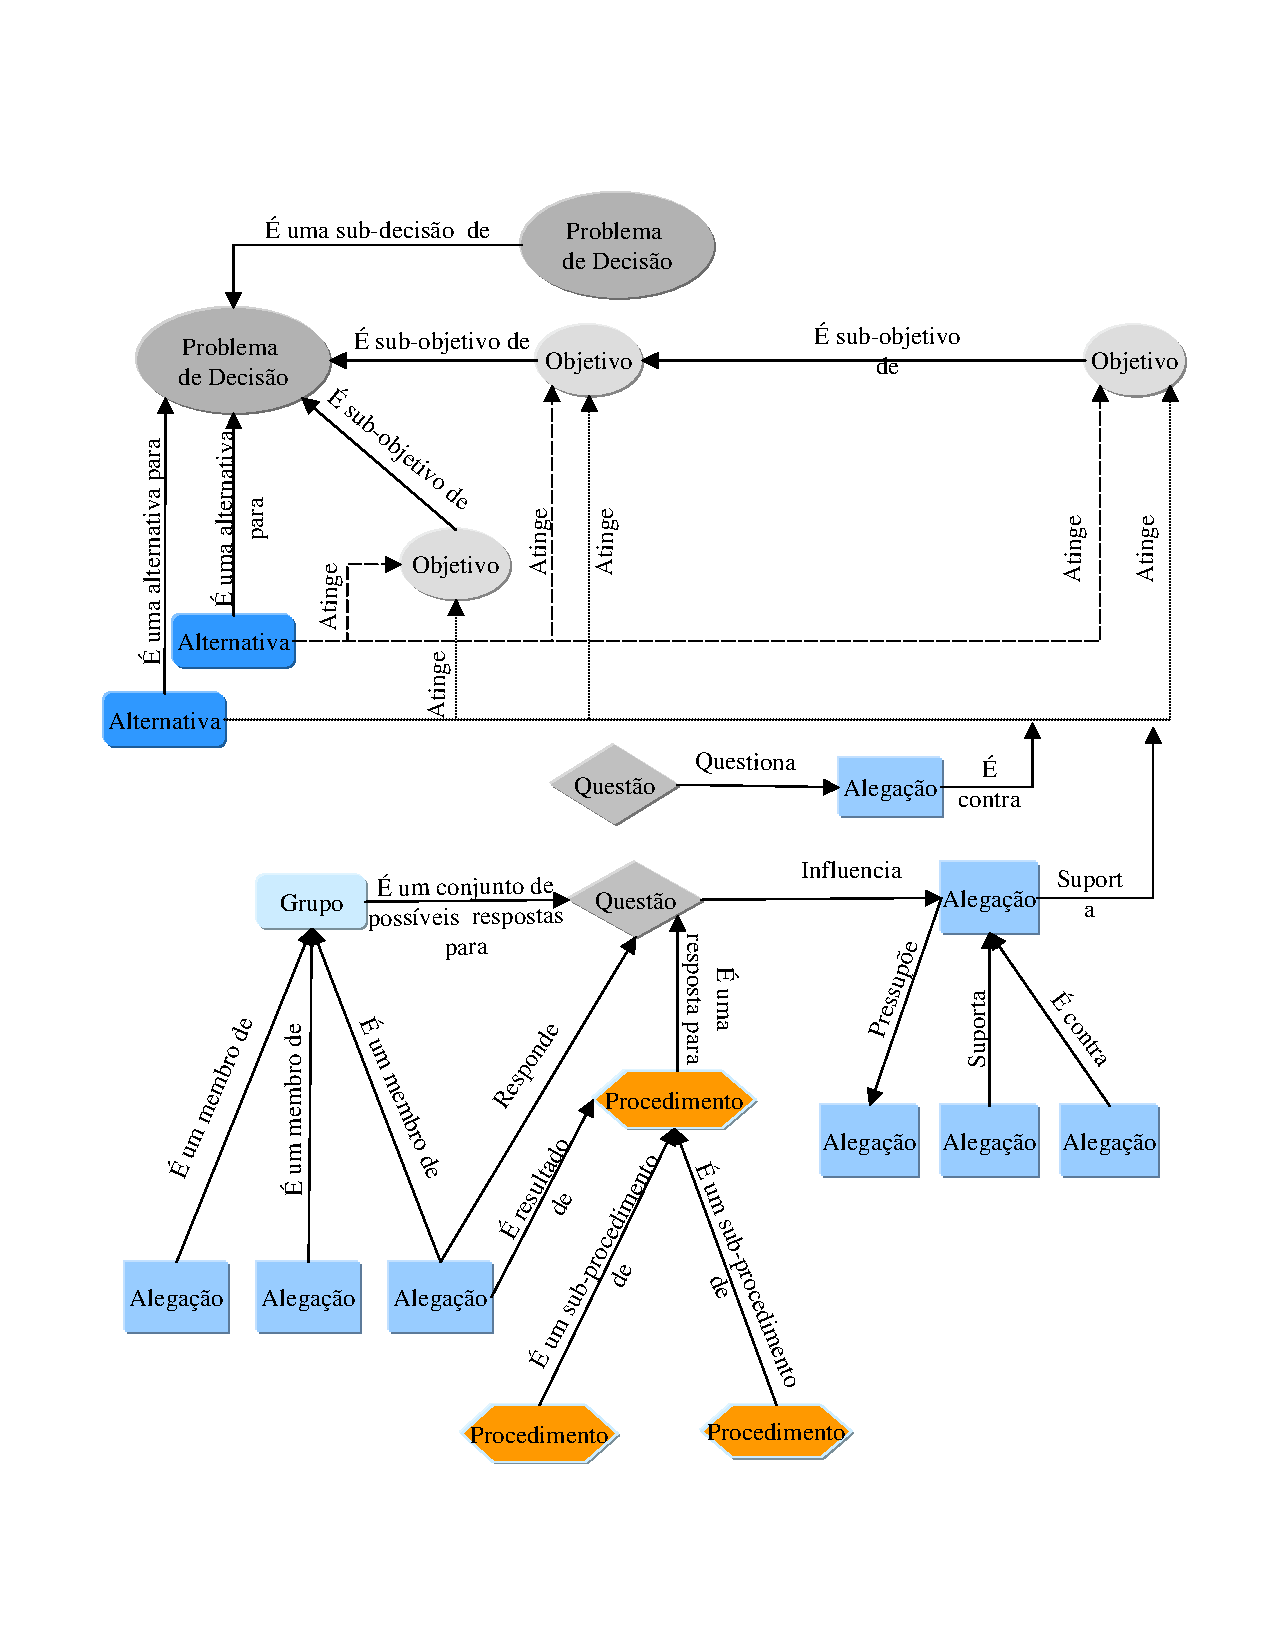
\includegraphics [width=13cm, height=11cm]{fDRL.pdf}
  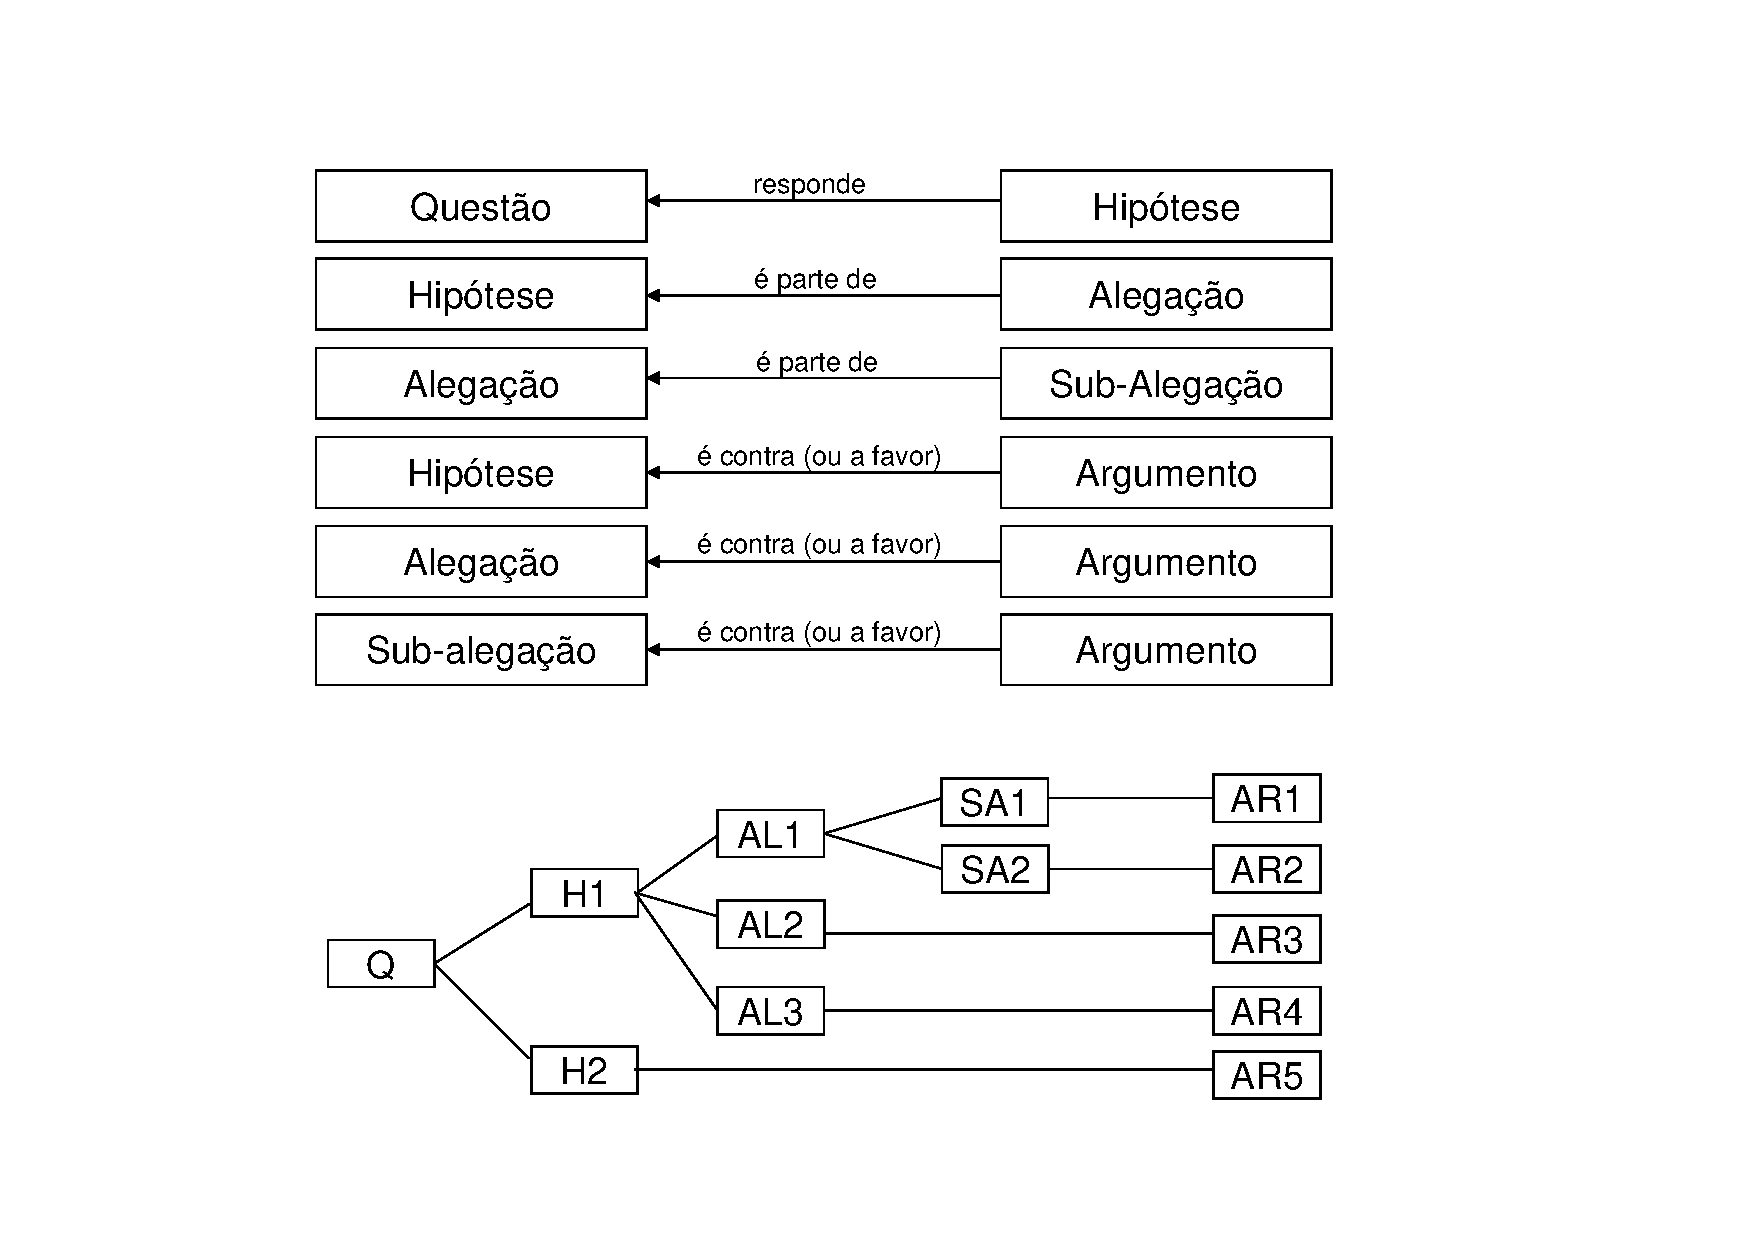
\includegraphics [width=0.75\textwidth, height= 9cm]{Kim.pdf}
  \caption {Representa��o de {\it design rationale} de acordo com a proposta de \cite{kim93}}
  \label{modeloKim}
\end{figure}

Comparando a proposta dos autores com o modelo IBIS e considerando
os exemplos de uso apresentados por Kim et al, � poss�vel notar
que:
\begin{itemize}
\item as entidades {\it quest�o} e {\it argumento} propostas no
modelo IBIS foram adotadas no modelo para o contexto de
pesquisa cient�fica e 
\item  h� uma rela��o entre {\it hip�tese} e
{\it posi��o}, ou seja, em ambos os modelos, o objetivo � indicar
poss�veis solu��es para uma quest�o gerada. 
\end{itemize}

O elemento novo na
proposta para o desenvolvimento de projetos de pesquisa s�o as
alega��es e sub-alega��es, que podem ser vistas como entidades que
favorecem o refinamento das hip�teses ou das alega��es, ou seja,
s�o utilizadas para tentar descrever a hip�tese em partes. Os
termos utilizados na elabora��o da proposta s�o usuais em contexto
de pesquisa.

Como aspecto positivo da proposta, pode ser mencionada sua
simplicidade e o fato de estar fortemente fundamentada em um
modelo de {\it design rationale} amplamente discutido. Como
aspectos negativos da proposta pode ser mencionado o fato de n�o
ter sido apresentado como os autores obtiveram o modelo adaptado,
ou seja, qual foi a motiva��o para o novo modelo e quais foram os
requisitos e as atividades cumpridas para a elabora��o da
proposta. Outro problema observado � que resultados experimentais
n�o foram indicados.

\section{Limita��es, perspectivas e desafios em {\it design rationale}}

Um dos resultados de uma pesquisa realizada recentemente, com oitenta e um projetistas de software, revelou que eles reconhecem a import�ncia em documentar {\it design rationale} na pr�tica e frequentemente usam as informa��es capturadas (em diferentes formatos) para analisar as decis�es tomadas durante o desenvolvimento dos projetos que participam. 
Al�m disso,  eles indicaram duas principais barreiras para a documenta��o e o uso de {\it design rationale}: 
\begin{enumerate} 
\item  falta de tempo para documenta��o das informa��es e 
\item  falta de padr�es e ferramentas apropriadas para o processo que envolve a captura de {\it design rationale}. 
\end{enumerate}

Em rela��o � segunda barreira mencionada, ficou evidente na pesquisa realizada que os participantes gostariam que padr�es e processos indicassem {\it porque}, {\it como}, {\it o que} e {\it quando} as informa��es de {\it design rationale} devem ser capturadas. Foi tamb�m obtido dos participantes que as ferramentas Microsoft (Word, Visio, Excel e Powerpoint) s�o geralmente utilizadas para a captura de {\it design rationale}, o que foi considerado um fator que os desmotiva para o uso da abordagem \citep{tang05}.

� importante notar que t�m surgido iniciativas em rela��o ao tratamento de {\it design rationale} por padr�es internacionais. O padr�o \cite{Ieee00} prop�e a associa��o de {\it design rationale} � descri��o da arquitetura de software e de sistemas. No entanto, � apresentada somente uma defini��o para a abordagem e n�o s�o indicados quais os tipos espec�ficos de informa��es devem ser capturadas. Em rela��o �s ferramentas para {\it design rationale}, nota-se que alguns trabalhos est�o sendo desenvolvidos no sentido de integr�-las a outras ferramentas comumente utilizadas no desenvolvimento de software, enfatizando as especificidades de cada fase \citep{Mye1999,van06,CanCasLuc2000}.

Uma tend�ncia que pode ser observada nas pesquisas mais atuais � o registro do {\it contexto} durante a captura de {\it design rationale}. O objetivo principal � promover a rastreabilidade, ou seja, fornecer informa��es que ajudem o projetista a entender, durante a recupera��o de {\it design rationale}, o cen�rio no qual a captura das informa��es ocorreu \citep{brei06,ngu06}. � poss�vel notar tamb�m que as pesquisas envolvendo {\it design rationale} privilegiam a abordagem da argumenta��o ainda hoje. A maioria dos estudos tentam propor varia��es dos modelos de representa��o, em particular do modelo IBIS.

\cite{hay06} apresentou alguns desafios de pesquisa na �rea para os pr�ximos anos. Segundo ele, � preciso investir esfor�os na captura ub�qua de {\it design rationale}, na investiga��o sobre possibilidades de uso de {\it design rationale} como um ve�culo para facilitar a transfer�ncia de tecnologia entre organiza��es e na realiza��o de estudos experimentais que contribuam para compor uma base de experi�ncias relativas a {\it design rationale}.

\section{Considera��es finais}

Neste cap�tulo foram apresentados conceitos e atividades relacionadas com a ado��o da abordagem de  {\it design rationale}. O uso dessa abordagem em diferentes contextos tamb�m foi enfatizada. 

A partir do estudo realizado, foi poss�vel conhecer as pesquisas que est�o sendo realizadas mais recentemente na �rea e os principais desafios para os pr�ximos anos. Al�m disso, essa revis�o biliogr�fica propiciou um referencial te�rico sobre o qual os resultados apresentados nesta tese contribuem, no sentido de apresentar a obten��o de uma base de experi�ncias envolvendo {\it design rationale}.

\chapter{Concep��o de um Processo para Projetos de Pesquisa em Software} \label{cap_concepcao}

\section{Considera��es iniciais}

Para a elabora��o do processo apresentado nesta tese, as atividades propostas por \cite{Hum95} em seu livro {\it A Discipline for Software Engineering}; Cap�tulo 13 ({\it Defining the Software Process}) foram consideradas como base. De forma geral, o autor sugere que um conjunto de etapas seja cumprido, mas n�o estabelece uma ordem obrigat�ria. 


%as seguintes etapas sejam executadas quando se pretende definir um processo de software (a sequ�ncia n�o � obrigat�ria): defini��o das necessidades e prioridades em rela��o � proposta de um novo processo, defini��o dos requisitos, dos objetivos e dos crit�rios de qualidade do processo, caracteriza��o dos processos comumente cumpridos no ambiente para o qual a proposta est� sendo elaborada, caracteriza��o do processo alvo, estabelecimento de uma estrat�gia de desenvolvimento do processo, defini��o do processo inicial, valida��o do processo obtido e realiza��o de melhorias. 

%\cite{dav94} enfatiza, tamb�m,
%que um processo deve ser projetado de modo a produzir resultados
%que satisfa�am �s exig�ncias dos clientes. Os objetivos de
%melhoria ou reengenharia de processos devem ser principalmente os
%do cliente e, assim, deve-se come�ar com um bom entendimento de
%quem s�o eles e quais s�o suas expectativas em rela��o ao
%processo.

Na se��o \ref{hump} � apresentada uma descri��o da abordagem proposta por Humphrey, que foi utilizada como fundamento te�rico. Nas se��es seguintes s�o apresentados os resultados do cumprimento das cinco primeiras etapas. Os resultados  da etapa de defini��o do processo s�o apresentados no Cap�tulo \ref{proc_pes}. Uma instancia��o do processo, observado como uma atividade inicial da valida��o, � apresentado na Se��o \ref{instancia}. A etapa 8 (melhorar o processo) n�o foi enfatizada neste trabalho.

\section{Proposta de Humphrey para defini��o de processos de software} \label{hump}

De acordo com \cite{Hum95}, processos de software devem ser propostos
quando n�o h� abordagens apropriadas para as necessidades
espec�ficas dos usu�rios interessados. A defini��o de processos
deve ser diretamente relacionada a ``o que'' o usu�rio precisa
fazer, ou seja, deve estar relacionada aos seus requisitos. Em geral, processos s�o utilizados quando o objetivo final
� executar alguma tarefa repetitiva. Processos de software tamb�m s�o importantes no sentido de auxiliar a
planejar e rastrear o trabalho, a guiar a execu��o e avalia��o das tarefas
e a propor melhorias. Foi sugerido que um processo contenha os seguintes elementos:

\begin{itemize}

\item {\it Scripts} que descrevam como o processo deve ser
colocado em pr�tica;

\item Formul�rios que auxiliem o registro dos dados que precisam
ser armazenados;

\item Padr�es para guiar o trabalho e fornecer uma base para
verifica��o da qualidade dos produtos e dos processos;

\item Alternativas para a melhoria do processo de forma a assegurar que
ele ir� continuar a satisfazer as necessidades dos seus
usu�rios, que evoluem constantemente.

\end{itemize}

A estrat�gia sugerida para a defini��o de processos de software �
semelhante aos modelos convencionais para o desenvolvimento de
produtos de software. Deve-se iniciar estabelecendo as
necessidades dos usu�rios e terminar com a realiza��o de testes
seguidos pela libera��o do processo. As atividades para a
defini��o de um processo s�o:

\begin{enumerate}

\item {\bf Determinar as necessidades e as prioridades}: envolve
determinar a natureza dos produtos que ser�o obtidos a partir da
execu��o do processo, identificar os principais atributos de cada
produto e as caracter�sticas do processo necess�rias para produzir
tais atributos.

\item {\bf Definir os objetivos do processo, as metas e os
crit�rios de qualidade}: envolve identificar o que os usu�rios
esperam do processo, os objetivos preliminares e as prioridades de
melhoria do processo.

\item {\bf Caracterizar o processo corrente}: para melhorar o
processo j� existente, � necess�rio compreender o processo
corrente e, em seguida, melhor�-lo de forma incremental. �
necess�rio descrever os principais passos, como est�o
relacionados, quais s�o os principais problemas observados pelos
usu�rios, se h� crit�rios de entrada e sa�da expl�citos e se �
poss�vel rastrear e realizar medi��es com o processo.

\item {\bf Caracterizar o processo alvo}: deve-se definir a
estrutura e identificar os principais elementos do processo.

\item {\bf Estabelecer uma estrat�gia de desenvolvimento do
processo}: est� relacionado � defini��o de ``como'' o processo
ser� definido.

\item {\bf Definir o processo inicial}: deve-se definir os {\it scripts},
os padr�es e os formul�rios para o processo inicial. Este processo
deve ser semelhante ao processo corrente, mas deve incluir
mudan�as que permitir�o aproximar do processo alvo. Sugere-se que
seja definido o processo como um todo, incluindo as diversas atividades. Em seguida, deve-se
definir um sub-processo para cada atividade.

\item {\bf Validar o processo inicial}: est� relacionado ao teste
do processo. Primeiramente, deve-se simular a execu��o do processo
usando dados de um projeto que tenha sido desenvolvido
recentemente. Se os dados necess�rios n�o estiverem dispon�veis, deve-se considerar aqueles que for poss�vel. Em seguida,
o processo deve ser utilizado no desenvolvimento de um pequeno projeto ou no desenvolvimento
de um prot�tipo.

\item {\bf Melhorar o processo}: ao utilizar o processo, as omiss�es e os problemas se tornar�o evidentes. As melhorias do processo se referem aos ajustes � primeira defini��o. � medida que os ajustes s�o feitos, a proposta converge para um processo inicial real�stico.

\end{enumerate}

\section{Determina��o das necessidades e das prioridades} \label{pro_nec}

\subsubsection{Sobre a natureza dos produtos que o processo dever� produzir}
Pretende-se elaborar um processo que seja �til para o
desenvolvimento de projetos de pesquisa. Em termos de produ��o de software, o processo ser� utilizado
para o desenvolvimento de prot�tipos, ou seja, n�o h� o interesse
no desenvolvimento de produtos de software\footnote{No desenvolvimento de prot�tipos nos projetos de pesquisa, os objetivos estrat�gicos s�o de investiga��o e obten��o de conhecimento. No desenvolvimento de produtos, a preocupa��o com os objetivos de neg�cio s�o evidentes.}. Al�m disso, o processo dever� ser �til para auxiliar o cumprimento de atividades e a produ��o de artefatos comuns ao desenvolvimento de projetos de pesquisa, tais como a elabora��o de um plano de pesquisa.

\subsubsection{Os principais atributos do produto}

Espera-se que os principais atributos dos produtos desenvolvidos utilizando o processo elaborado sejam simplicidade, flexibilidade e manutenibilidade.

%Espera-se que os artefatos produzidos utilizando o processo elaborado sejam simples e auxiliem a evolu��o de projetos de pesquisa.

%\subsection{Determinar as prioridades dos atributos do produto}
%Acho que nao precisa colocar esta se�ao.

\subsubsection{Sobre as caracter�sticas necess�rias do processo para produzir os atributos do produto}
\label{cara}

%Elementos importantes destacados na literatura para auxiliar a manutenibilidade de software s�o: elaborar e manter documenta��o completa e atualizada, projetar sistemas de forma que os componentes possuam alta coes�o e baixo acoplamento, �construir qualidade� desde o in�cio do projeto e fazer o gerenciamento de configura��o de software.

A documenta��o compreens�vel e consistente das informa��es
relevantes de um projeto � fundamental quando outras pessoas que
n�o participaram do desenvolvimento precisam entender os artefatos
produzidos \citep{sch87}. Assim, considerando-se que a alta
rotatividade dos membros e a identifica��o iterativa dos requisitos s�o caracter�sticas importantes do
desenvolvimento dos projetos de pesquisa, o processo dever�
enfatizar a documenta��o simples, compreens�vel e propensa a mudan�as. Com isso, busca-se garantir que n�o somente o c�digo, mas tamb�m a documenta��o,  estejam dispon�veis quando os estudantes e os pesquisadores deixam de fazer parte da equipe e outras pessoas passam a trabalhar na continuidade dos projetos. 

%entra na parte de caracteristicas de qualidade.

%Processos de software precisam ser, sobretudo, compreens�veis e simples \cite{Hum95}. Estes requisitos foram considerados na elabora��o do processo apresentado nesta tese. Considerou-se a possibilidade de que os membros das equipes que desenvolvem projetos de software n�o sejam experientes na aplica��o de processos de software e, dessa forma, apresentar um processo que possa ser facilmente compreens�vel � um fator relevante para motivar sua aplica��o.

 
%De acordo com Nielsen \cite{Nil93}, no contexto de interfaceshomem-computador, o conceito de simplicidade est� relacionado � apresenta��o de informa��es que os usu�rios realmente necessitam. McCall et al \cite{McC77} definem simplicidade como o quanto um programa pode ser entendido sem dificuldade. Estes conceitos podem ser utilizados em rela��o a processos de software, ou seja, os usu�rios devem ser solicitados a cumprir as atividades e gerar os artefatos que sejam de fato importantes para o estado atual do projeto e, al�m disso, o processo deve ser f�cil de entender e de usar. M�tricas que auxiliam a avalia��o deste fator s�o apresentadas no Anexo 3.



%O fator manutenibilidade pode ser considerado sob diferentes perspectivas.

%Pretende-se obter artefatos que sejam simples. De acordo com Nielsen \cite{Nil93}, no contexto de interfaces homem-computador, o conceito de simplicidade est� relacionado � apresenta��o de informa��es que os usu�rios realmente necessitam. Este conceito pode ser utilizado em rela��o a processos de software, ou seja, os usu�rios devem ser solicitados a cumprir as atividades e gerar os artefatos que sejam de fato relevantes para o estado atual do projeto.

%Al�m disso, pretende-se que os artefatos sejam �teis para auxiliar a evolu��o do projetos de pesquisa. O termo evolu��o est� relacionado � continuidade dos projetos de pesquisa. Nesse sentido, pretende-se fornecer um processo que valorize a ``constru��o da qualidade'' desde o in�cio do projeto, conforme indicado por X. Isso envolve valorizar, por exemplo, a documenta��o dos projetos a as atividades de garantia de qualidade.

\subsubsection{O relacionamento entre caracter�sticas do processo e atributos do produto (fraca, m�dia ou forte)}

Observa-se um forte relacionamento.



\section{Defini��o de objetivos, metas e crit�rios de qualidade do processo} \label{obj}

De acordo com Humphrey, � fundamental identificar o que se espera
obter com o processo que ser� projetado, ou seja, quais s�o as
necessidades das pessoas que usar�o o processo. De forma similar, \cite{dav94}
observou que um dos primeiros passos na defini��o de um processo � explicitar quem s�o os seus
ou usu�rios e o que eles esperam obter. Os autores ressaltam
a import�ncia em rela��o ao projeto de processos que satisfa�am de
fato �s exig�ncias do(s) usu�rio(s).

De forma geral, o objetivo da proposta est� relacionado com: (1) a obten��o de melhorias na documenta��o de projetos de pesquisa envolvendo software, de forma a contribuir para a continuidade e evolu��o dos mesmos e (2) a organiza��o das atividades cumpridas e artefatos gerados, de forma a contribuir para a reprodu��o de colabora��es bem sucedidas. 

Os seguintes usu�rios foram considerados para a defini��o do processo apresentado neste trabalho:

\begin{enumerate}
\item pesquisadores (estudantes e colaboradores);

\item coordenadores de projetos;

\item profissionais do setor industrial interessados em estabelecer parcerias com
universidades.

%\item institui��es financiadoras de projetos de pesquisa
\end{enumerate}

Conforme apresentado na sub-se��o seguinte, nesta etapa da concep��o do processo buscou-se, primordialmente, identificar o que os usu�rios esperam do processo, ou seja, definir os requisitos da proposta.

Para a identifica��o dos requisitos dos usu�rios do processo foi
realizada revis�o da literatura. N�o foi poss�vel fazer a
distin��o entre requisitos dos pesquisadores e requisitos dos coordenadores
dos projetos e, portanto, eles s�o apresentados indistintamente a
seguir.



%De forma geral, observou-se que os estudantes esperam receber projetos documentados quando precisam dar continuidade aos projetos; os coordenadores esperam que o gerenciamento dos projetos ocorra de forma efetiva; as empresas esperam receber treinamento e capacita��o e transfer�ncia de conhecimento e de tecnologia e as institui��es financiadoras esperam os resultados cient�ficos do projeto desenvolvido.


%- Clientes do processo academico \\
%- estudantes; esperam documenta��o dos projetos (questionario sobre manuten��o), \\
%- coordenadores de projetos; esperam gerenciamento dos projetos (questionario com professores)\\
%- empresas; esperam treinamento e capacita��o, transferencia de conhecimento e de tecnologia\\
%-Institui��es financiadoras, desenvolvimento de projetos de pesquisa, presta��o de contas, gerenciamento de recursos, gerenciamento de recursos financeiros esperam relatorio de presta��o de contas, relatorios cientificos, teses, disserta��es.\\


%outros clientes (nao estou considerando): \\
%-administrativos -- n�o estou considerando\\
%-Institui��es de ensino: esperam desenvolvimento de projetos de pesquisa e cumprimento de prazos. Esperam receber relatorios cient�ficos e de atividades, teses, disserta��es\\
%- candidatos a participa��o de grupos de pesquisa (alunos de p�s gradua��o) -- esperam um cronograma com datas de submissao de documentos, resultados, matriculas. Isso envolve todo o processo de sele��o de alunos\\
%- secret�rios, esperam um processo de aquisi��o de software, equipamentos, materiais\\
%- avaliadores do projeto, que podem ser os membros de uma banca ou avaliadores dos orgaos de pesquisa.

%As organiza��es precisam definir um respons�vel pelo funcionamento de cada processo como um todo (process owner).

%2)- Savi e Franzoni indicaram que para o modelo de referencia ser construido foi necessario saber, antes de tudo, quais os processos normalmente existem na incubadora (no meu caso, no ambiente academico)


\subsubsection {Usu�rios: pesquisadores e coordenadores de projetos}

\begin{enumerate}

\item Requisito (o que esperam): \textit{Atividades de pr�-desenvolvimento.} Fonte:  \cite{Rob98,Amb04,wal03,DuSoBuRe04,Hwa06}

\begin{description}

\item [Processos:] defini��o do tema e planejamento do
projeto de pesquisa, treinamento (no dom�nio da aplica��o e outros
temas de interesse dos pesquisadores) 

\end{description}

\item Requisito (o que esperam): \textit{Atividades de ciclo de vida.}  Fonte: \cite{Amb04,Hwa06,Rob98,seg05}

\begin{description}

\item [Processos:] an�lise de requisitos, projeto, gera��o de
c�digo, testes

\item Observa��o: deve-se ressaltar tamb�m que, em rela��o �s atividades de ciclo de vida, a combina��o entre m�todos �geis e abordagens tradicionais, o uso do m�todo da prototipa��o e do desenvolvimento iterativo tamb�m foram enfatizados por \cite{seg05} e por \cite{Carl02}.  

\end{description}

\item Requisito (o que esperam): \textit{Atividades de gerenciamento.} Fonte: \cite{Rob98,Amb04,Oli05,wal03,DuSoBuRe04,Bol04,conn04,numpra03,uwa06,Hwa06}

\begin{description}

\item [Processos:] gerenciamento de tarefas, cronograma, custos, recursos, riscos, configura��o e infra-estrutura
\end{description}

\item Requisito (o que esperam): \textit{Atividades de garantia de qualidade de software.} Fonte: \cite{Rob98,Amb04,Oli05,alp05,cav89,wal03,conn04,Hwa06}

\begin{description}

\item [Processos:] verifica��o, valida��o, documenta��o,
revis�o t�cnica, controle de altera��es, 
revis�o por pares, medi��es em produtos e processos (envolve garantia de qualidade de artefatos de software e outros artefatos resultantes do trabalho de pesquisa)

\end{description}

\item Requisito (o que esperam): \textit{Atividades de apoio ao desenvolvimento
colaborativo.} Fonte: \cite{Amb04,Oli05,seg05,alp05,Carl02,Bol04,numpra03,Wal,uwa06,rog98,suc04}


\begin{description}

\item [Processos:] apoio � comunica��o, defini��o de pap�is, representa��o do processo cumprido e dos pontos de colabora��o que devem
ser compartilhados entre os membros do grupo, integra��o de c�digo
e de outros artefatos, coordena��o das atividades,
registro do conhecimento comum ao grupo e percep��o do grupo em
rela��o ao contexto de trabalho

\end{description}

\item Requisito (o que esperam): \textit{Atividades de apoio ao desenvolvimento
distribu�do.} Fonte: \cite{Oli05,seg05,alp05,Amb04,bez99,suc04,per97}

\begin{description}

\item [Processos:] apoio � comunica��o, ao
acesso ao conhecimento, � realiza��o de atividades cooperativas, ao registro de experi�ncias e discuss�es,
� identifica��o de habilidades, experi�ncias e recursos humanos,
tecnol�gicos e econ�micos de cada equipe;  coordena��o
distribu�da (por um coordenador local) e  ger�ncia distribu�da do
projeto, controle de artefatos (acompanhamento do
desenvolvimento de artefatos) e  resolu��o de problemas

\end{description}

\item Requisito (o que esperam): \textit{Atividades de apoio ao desenvolvimento de pesquisas.} Fonte: \cite{seg05,alp05,Carl02,wal03,Bol04,conn04,AthPlo2000,Oli05}


\begin{description}

\item [Processos:] divulga��o do projeto, {\it
postmortem}, apoio � revis�o da literatura, � realiza��o de
entrevistas e {\it surveys}, � execu��o de experimentos, �
reda��o de documentos t�cnicos, � elabora��o e disponibiliza��o de material did�tico

\end{description}
\end{enumerate}


\subsubsection {Usu�rios: profissionais do setor industrial}

\begin{enumerate}

\item Requisito (o que esperam): \textit{Atividades de apoio � transfer�ncia de conhecimento}
(boas pr�ticas de Engenharia de Software). Fonte: \cite{Korn03,rog98,Ros05,Jen04,beck97}

\begin{description}

\item [Processos:] elabora��o de material para treinamento, sele��o
de parceiro, negocia��o de suporte financeiro para universidade e
bolsa de estudos para estudantes envolvidos, planejamento de est�gio de estudantes e pesquisadores na ind�stria,
planejamento de est�gio de profissionais na universidade, cria��o de infra-estrutura na universidade, transfer�ncia de solu��es e tecnologias para o parceiro da ind�stria, elabora��o de plano de
opera��o (detalhes do projeto de pesquisa, m�todos, pessoas,
t�cnicas e artefatos a serem produzidos), defini��o de pap�is e
responsabilidades, submiss�o de proposta � ag�ncia financiadora, avalia��es dos parceiros envolvidos
em rela��o aos resultados obtidos, captura e reuso de conhecimento
\end{description}

\item Requisito (o que esperam): \textit{Atividades de apoio � forma��o de parcerias universidade-ind�stria}. Fonte: \cite{chan90,Mac96,Korn03,Wal,Hwa06,ell}

\begin{description}

\item [Processos:] defini��o de objetivos claros, identifica��o dos benef�cios que
cada participante ter� com a parceria, planejamento e gerenciamento do projeto, apoio � comunica��o entre os participantes,
estabelecimento de acordo sobre confidencialidade de
informa��es, sele��o de informa��es que ser�o
disponibilizadas na parceria, negocia��o de suporte
financeiro, identifica��o de recursos fornecidos por cada uma das
partes envolvidas, gera��o de relat�rios e documentos pelo
pesquisador respons�vel sobre o funcionamento de laborat�rios,
rela��es entre academia e ind�stria e elabora��o de contratos
incluindo direitos de propriedade do software ({\it copyrights} e
patentes), direito de publica��o dos resultados obtidos, propriedade intelectual, divis�o de lucros, controle da
especifica��o dos projetos

%\item Produtos: material did�tico, relat�rios t�cnicos, contratos

\end{description}
\end{enumerate}

Em s�ntese, os requisitos observados na literatura foram divididos em 9 �reas: atividades de
pr�-desenvolvimento, de ciclo de vida, de gerenciamento, de garantia de qualidade de software, de apoio ao desenvolvimento
colaborativo, de apoio ao desenvolvimento distribu�do, de apoio ao desenvolvimento de pesquisas, de apoio � transfer�ncia de conhecimento e de apoio � forma��o de parcerias universidade-ind�stria. Nota-se que as �reas cobertas pela norma \cite{ISO12207} foram abordadas pelos pesquisadores, o que motivou a redefini��o dos processos apresentados na norma. Al�m disso, houve a inser��o de novos processos, para atender ao dom�nio do desenvolvimento de pesquisas. 

\subsubsection{Sobre os crit�rios de qualidade do processo}

De acordo com a proposta de Humphrey, � fundamental definir os
crit�rios de qualidade do processo que dever�o servir como base
para permitir caracterizar o que � um bom ou um mau processo.
O autor prop�e que, primordialmente, um
processo possa ser entendido e usado facilmente. Estes atributos foram considerados como crit�rio de qualidade para o processo proposto. Assim, foram definidas m�tricas
que pudessem ser utilizadas para avali�-los. 

Os atributos e as m�tricas apresentadas a seguir foram adapta��es da norma \cite{ISO9126a} (que trata a avalia��o de produtos de software) para o contexto de avalia��o de processos. \\

\begin{enumerate}
\item {\bf Facilidade de entendimento}

\noindent {\it Defini��o do atributo}: Facilidade com que as descri��es do processo podem ser entendidas. 

\noindent {\it Proposta de avalia��o}: -- O processo � f�cil de entender?

\noindent {\it Origem}: Norma ISO/IEC 9126, parte 2 (m�tricas externas), caracter�stica usabilidade, subcaracter�stica intelegibilidade.  

\noindent {\it M�todo de aplica��o e m�tricas}: Este atributo pode ser avaliado cumprindo-se tr�s tarefas, conforme descritas a seguir. 

\begin{description} 
\item [Tarefa 1:] treine usu�rios e fa�a entrevistas ou observe seus comportamentos. Conte o n�mero de atividades do processo que foram compreendidas adequadamente e compare com o n�mero total de atividades consideradas no treinamento. 

\begin{itemize}
\item {\bf M�trica:}  X = A/NA \\
 A = n�mero de atividades no treinamento cuja proposta � compreendida corretamente pelo usu�rio; NA = n�mero total de atividades; X � um valor absoluto.
\item {\bf Interpreta��o do resultado:} 0 $\leq$ X $\leq$ 1. \\
 O valor � considerado melhor quanto mais pr�ximo X estiver de 1. 
\end{itemize}

\item [Tarefa 2:] treine usu�rio e fa�a entrevistas ou observe seus comportamentos. Conte o n�mero de atividades cujas entradas e sa�das foram compreendidas corretamente e compare com o n�mero total de atividades consideradas no treinamento.   

\begin{itemize}
\item {\bf M�trica:} Y = B/NA \\
 B = n�mero de atividades no treinamento cujas entradas e sa�das foram compreendidas corretamente; NA = n�mero total de atividades; Y � um valor absoluto.
\item {\bf Interpreta��o do resultado:} 0 $\leq$ Y $\leq$ 1. \\
 \textnormal{O valor � considerado melhor quanto mais pr�ximo Y estiver de 1.} 
\end{itemize}

\item [Tarefa 3:] realize experimenta��o com o processo ap�s o treinamento com o usu�rio. Conte o n�mero de atividades cumpridas corretamente e compare com o n�mero total de atividades que fizeram parte do experimento. 

\begin{itemize}
\item {\bf M�trica:} Z = C/NA \\
 C = n�mero de atividades completadas com sucesso na experimenta��o do processo; NA = n�mero total de atividades; Z � um valor absoluto.
\item {\bf Interpreta��o do resultado:} 0 $\leq$ Z $\leq$ 1. \\  
 \textnormal{O valor � considerado melhor quanto mais pr�ximo Z estiver de 1.}
 \end{itemize}

\end{description}

\item {\bf Facilidade de uso}

\noindent {\it Defini��o do atributo}: Facilidade com que o processo pode ser utilizado.  

\noindent {\it Proposta de avalia��o}: -- O processo � f�cil de usar? 

\noindent {\it Origem}: Norma ISO/IEC 9126, parte 2 (m�tricas externas), caracter�stica usabilidade, subcaracter�stica operacionalidade.  

\noindent {\it M�todo de aplica��o e m�tricas}: Este atributo pode ser avaliado cumprindo-se 3 tarefas, conforme descritas a seguir.

\begin{description}
\item [Tarefa 1:] realize experimenta��o com o processo ap�s o treinamento com o usu�rio. Fa�a entrevistas com foco na consist�ncia da descri��o do processo. Conte o n�mero de atividades do processo nas quais o usu�rio encontra inconsist�ncias inaceit�veis e compare com o n�mero total de atividades consideradas no experimento.

\begin{itemize}
\item {\bf M�trica:} X = 1 - A/NA \\
 A = n�mero de atividades do processo nas quais o usu�rio encontra inconsist�ncias inaceit�veis; NA = n�mero total de atividades; X � um valor absoluto.  
\item {\bf Interpreta��o do resultado:} 0 $\leq$ X $\leq$ 1. \\
 \textnormal{O valor � considerado melhor quanto mais pr�ximo X estiver de 1.}  
\end{itemize}


\item [Tarefa 2:] realize atividades de experimenta��o do processo ap�s o treinamento e observe o comportamento do usu�rio. Conte o n�mero de vezes que o usu�rio pausa por um longo per�odo ou falha repetidamente na mesma opera��o devido a dificuldades na compreens�o da descri��o do processo e compare com o n�mero total de atividades consideradas no experimento. 

\begin{itemize}
\item {\bf M�trica:} Y = B/TO \\
 B = n�mero de vezes o usu�rio pausa por um longo per�odo ou falha repetidamente na mesma opera��o devido a dificuldades na compreens�o das mensagens; TO = tempo de observa��o; Y � um valor do tipo raz�o.
\item {\bf Interpreta��o do resultado:} Y $\geq$ 0. \\
 \textnormal{O valor � considerado melhor quanto mais pr�ximo Y estiver de 0.} 
\end{itemize}


\item [Tarefa 3:] realize atividades de experimenta��o do processo ap�s o treinamento e observe o comportamento do usu�rio. Conte o n�mero de atividades que o usu�rio customiza de forma bem sucedida e o n�mero de tentativas de customiza��o e compare com o n�mero total de atividades consideradas no experimento.  

\begin{itemize}
\item {\bf M�trica:} Z = C/TC \\
 C = n�mero atividades customizadas com sucesso; TC = n�mero de tentativas de customiza��o; Z � um valor absoluto.
\item {\bf Interpreta��o do resultado:} O $\leq$ Z $\leq$ 1.  \\
 \textnormal{O valor � considerado melhor quanto mais pr�ximo Z estiver de 1.} 

\end{itemize}

\end{description}

\end{enumerate}





\section{Caracteriza��o do processo atual} \label{atual}

De acordo com Humphrey, as chances de se conseguir resultados
positivos s�o maiores quando h� planos para a realiza��o de v�rias
mudan�as incrementais em um processo j� existente, ao inv�s de uma �nica mudan�a dr�stica.
Assim, n�o � vi�vel definir um processo completamente novo em que sejam
desconsideras as pr�ticas adotadas pela comunidade que
executa o processo. O autor sugere, portanto, que se
conhe�a o processo que � cumprido e que se deseja melhorar. Para
isso, alguns pontos principais precisam ser avaliados, ou seja, �
preciso descrever as principais atividades cumpridas pelo processo
atual, como est�o relacionadas, o tempo gasto para cumprir cada
uma delas, os problemas encontrados, os crit�rios de entrada e sa�da e os planejamentos e as
medi��es que s�o realizadas com a execu��o do processo atual.

%O processo cumprido para o desenvolvimento do projeto SAFE �
%utilizado para caracteriza��o do processo atual, sendo apresentado
%na pr�xima subse��o. Sob outra perspectiva, a participa��o e a
%experi�ncia no projeto SAFE foram fundamentais para a elabora��o do
%processo apresentado, servindo como um estudo de caso que precedeu a
%elabora��o do projeto.


%Buscou-se identificar o processo cumprido no desenvolvimento de projetos de pesquisa por meio de revis�o da literatura, ou seja, foram buscados documentos cient�ficos que tratassem os processos utilizados nos n�cleos de pesquisa. No entanto, poucos documentos cient�ficos foram encontrados \citep{numpra03,wal03}, o que tornou invi�vel a caracteriza��o do processo utilizado atualmente para o desenvolvimento de pesquisas.

A abordagem utilizada foi a de analisar pr�ticas cumpridas
registradas em artigos cient�ficos no contexto de projetos de
pesquisa. Foi poss�vel identificar somente pr�ticas de desenvolvimento de software, e n�o pr�ticas mais gen�ricas de desenvolvimento de projetos de pesquisa. Foram analisados documentos de 36 projetos que inclu�ram
produ��o de software, que foram desenvolvidos em
diferentes pa�ses e cujas publica��es foram reportadas na literatura
nos �ltimos cinco anos. Resumos foram evitados, por fornecerem
apenas uma descri��o breve do projeto. Os documentos foram
buscados em peri�dicos, anais, teses, disserta��es e reposit�rios
de projetos na internet. � importante observar que uma amea�a a
validade dos resultados obtidos se refere ao fato de que os
documentos analisados n�o tinham como objetivo descrever o
processo utilizado e, portanto, � poss�vel que somente uma parte
das atividades cumpridas tenham sido apresentadas. Al�m disso, n�o
foi poss�vel inferir o quanto os processos foram cumpridos. Os
resultados obtidos s�o apresentados na Figura \ref{gra_corrente}
em termos de porcentagem do cumprimento das pr�ticas em rela��o ao
n�mero total de projetos avaliados. No eixo horizontal s�o
apresentadas as atividades mais indicadas nos documentos
analisados e no eixo vertical s�o apresentadas as porcentagens. A
rela��o entre os projetos analisados e as pr�ticas cumpridas �
apresentada no Ap�ndice 1.

\begin{figure} [!ht]
 \centering
  \bfseries
  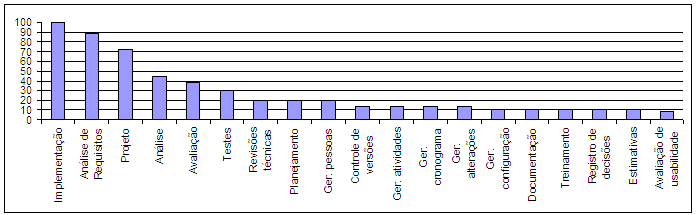
\includegraphics [width=0.99\textwidth]{grafico.png}
  \caption{Pr�ticas cumpridas no desenvolvimento de 36 projetos de pesquisa (em termos de porcentagem)}
  \label{gra_corrente}
\end{figure}

Pelo resultado apresentado no gr�fico � poss�vel notar que, por se tratarem de projetos de software, 100\% dos projetos mencionaram implementa��o. As atividades cumpridas por pelo menos 50\% dos projetos foram an�lise de requisitos e projeto. O resultado obtido foi utilizado na elabora��o do processo proposto neste trabalho de duas formas:
\begin{description}
\item [(a)] balancear requisitos dos usu�rios e atividades conhecidas por eles para a elabora��o do processo e 
\item [(b)] colaborar na indica��o de atividades em que estudos adicionais sobre melhorias na documenta��o (tendo em vista a melhoria da manuten��o dos projetos) seriam realizados, considerando a abordagem de {\it design rationale}. 
\end{description}

Humphrey sugere que a melhoria de um processo seja iniciada por atividades que s�o conhecidas pelos usu�rios do processo.  \cite{Roc01} apresentaram um exemplo de defini��o de processos em que essa estrat�gia foi utilizada na pr�tica e os resultados obtidos foram positivos.

Uma revis�o da literatura foi conduzida, com o objetivo de coletar dados sobre as pr�ticas gen�ricas de desenvolvimento de projetos de pesquisa envolvendo software (atividades al�m daquelas de ciclo de vida de software). Em resumo, foi poss�vel observar que: 

\begin{itemize}

\item Poucas atividades referentes a planejamento e controle s�o cumpridas, pois h� muitas incertezas em rela��o ao desenvolvimento de projetos de pesquisa. H� incertezas, por exemplo, em rela��o a: (1) o tempo gasto para provar uma teoria ou obter resultados v�lidos para experimentos e (2) os requisitos que ser�o considerados no desenvolvimento do projeto, pois eles s�o identificados gradualmente, a medida em que o projeto � desenvolvido e os resultados s�o percebidos \citep{hul05};

\item A documenta��o gerada nos projetos de pesquisa n�o � ideal pois, em geral, est� restrita a documentos cient�ficos, como artigos, disserta��es e teses \citep{wal03,Bol04};

\item H� alta rotatividade dos membros que participam do desenvolvimento de projetos de pesquisas e nem sempre a documenta��o dispon�vel � adequada para que novos participantes possam entender o est�gio em que o projeto se encontra \citep{numpra04,cav89}.

\item As atividades relacionadas a treinamento geralmente ocorrem de formas diferentes, de acordo com o contexto em que � realizado. Em geral, o treinamento em ambiente acad�mico ocorre por meio de uma combina��o de aulas e tutorias e n�o h� envolvimento em termos pr�ticos dos participantes com o conte�do apresentado.  No contexto industrial, � comum que aulas breves sejam ministradas e trabalhos pr�ticos sejam desenvolvidos por pequenos grupos \citep{Ble05}.

\end{itemize}

Durante a etapa de caracteriza��o do processo corrente,  Humphrey ainda sugere que algumas quest�es sejam respondidas. Para responder as quest�es, foram considerados, principalmente, os dados apresentados nesta se��o. As respostas representam tamb�m um resumo sobre as caracter�sticas do desenvolvimento de projetos de pesquisa apresentadas em outras se��es.

\begin{enumerate}

\item {\it � poss�vel descrever as principais atividades do
processo corrente, como est�o relacionadas e o tempo gasto para
execu��o de cada uma delas?} \\
 De forma geral observou-se que s�o
executadas principalmente atividades de ciclo de vida de desenvolvimento de software, destacando-se: implementa��o, an�lise de requisitos e projeto. N�o foram encontradas informa��es sobre o relacionamento entre as
atividades e o tempo gasto para execut�-las.

\item {\it H� problemas relacionados aos processos correntes?
Liste-os}. \\ 
H� dificuldades na manuten��o
dos projetos. � comum a re-escrita (ao inv�s da evolu��o) de
funcionalidades dos prot�tipos.
\cite{Bol04} e \cite{wal03} destacam as limita��es na
documenta��o gerada nos projetos, que � um dos principais fatores
que dificultam a continuidade dos mesmos. Problemas com o
gerenciamento de projetos, principalmente quando s�o desenvolvidos
de forma distribu�da, foram indicados por
\cite{cav02} e \cite{uwa06}. Observam-se tamb�m
problemas no estabelecimento de parcerias entre ind�stria e
academia, devido a dificuldades na defini��o de objetivos e de pap�is e no gerenciamento de recursos \citep{Korn03}.

\item {\it Os passos do processo corrente possuem artefatos de
entrada e de sa�da bem definidos?} \\
 N�o foram encontrados registros
que pudessem indicar tais crit�rios.

\item {\it O processo corrente � planejado e rastreado?} \\
N�o. Conforme apresentado por \cite{hul05}, na pr�tica,
poucas atividades de planejamento de projetos de pesquisa s�o
realizadas ou, pelo menos, reportadas. Os autores consideram tamb�m que as diferen�as entre o
desenvolvimento de projetos de pesquisa e o desenvolvimento de software na ind�stria imp�em que o gerenciamento
dos projetos ocorra de forma diferenciada em ambos os casos.

\item {\it S�o realizadas medi��es suficientemente no processo corrente de forma
a possibilitar que planos de melhoria sejam propostos?} \\
Foram encontrados alguns relatos que indicam interesse da
comunidade cient�fica em medir os processos utilizados nos
laborat�rios de pesquisa. \cite{coc03,cocc01} prop�s um modelo, aplicado em duzentos
institutos, para coleta de dados sobre desempenho e
produtividade em laborat�rios de pesquisa. As m�tricas estabelecidas no modelo est�o relacionadas a: (1) {\it auto
financiamento}, que � a quantidade de recursos obtidos a partir da
parceria entre universidade e ind�stria; (2) {\it treinamento}, que � a
quantidade de pessoas treinadas no instituto, por exemplo, n�mero
de pessoas que obtiveram alguma titula��o e n�mero de pessoas que
participaram de cursos tempor�rios; (3) {\it ensino}, que � a
quantidade de cursos oferecidos no instituto e (4) {\it
produ��o cient�fica}, que � a quantidade de artigos publicados em
peri�dicos nacionais e internacionais. Outras iniciativas e
experi�ncias tamb�m foram apresentadas \citep{har94,luw99}, no
entanto, n�o foi discutida a rela��o entre a aplica��o de
m�tricas e melhoria dos processos. Em outros estudos, a �nfase
est� no processo de avalia��o utilizado e h� pouca discuss�o
sobre as medi��es realizadas \citep{wal03,miy98}. Nestes casos, s�o
apresentadas rela��es entre as avalia��es e a melhoria dos
processos. De forma geral, nota-se que h� iniciativas no sentido
de medir, avaliar e melhorar os processos utilizados no
desenvolvimento de pesquisas. N�o foram encontradas, por�m, generaliza��es sobre medi��es que pudessem indicar como poss�veis planos de melhoria podem ser implantados.


\end{enumerate}






\section{Caracteriza��o do processo almejado} \label{alvo}

De acordo com Humphrey, nesta etapa deve-se identificar os objetivos a serem alcan�ados em rela��o ao processo que est� sendo proposto, bem como a estrutura e os principais elementos do processo.

Para a apresenta��o do processo padr�o foi utilizada a estrutura indicada na norma ISO/IEC 12207, em que os processos s�o divididos em processos fundamentais, processos de apoio e processos organizacionais. Assim, a estrutura geral do processo almejado p�de ser ent�o definida: 

\begin{description}
\item [1. Processos Fundamentais:]   \sffamily Processo de aquisi��o,  Processo de inicia��o,    Processo de desenvolvimento,   Processo  de opera��o,  Processo  de manuten��o.
 
\normalfont
\item [2. Processos de Apoio:]  \sffamily Processo de documenta��o,  Processo de ger�ncia de configura��o,  Processo de garantia da qualidade,  Processo de verifica��o,  Processo de valida��o,  Processo de revis�o,  Processo de resolu��o de problemas,  Processo de revis�o sistem�tica,  Processo de prepara��o de documentos cient�ficos,  Processo de elabora��o de m�dulos educacionais,  Processo de {\it postmortem} e Processo de transfer�ncia tecnol�gica.

\normalfont
\item [3. Processos Organizacionais:]  \sffamily Processo de treinamento, Processo de ger�ncia, Processo de infra-estrutura, Processo de melhoria, Processo de planejamento, Processo de divulga��o, Processo de comunica��o, Processo de coordena��o e Processo de estabelecimento de parceria universidade-empresa.

\end{description}

\normalfont

\section{Estabelecimento de uma estrat�gia de desenvolvimento do
processo} \label{estrat}

De acordo com Humphrey, nesta etapa a(s) pessoa(s) respons�vel(is)
pela defini��o do processo deve(m) definir e cumprir tarefas que a(s)
auxilie(m) a conhecer os processos. Algumas
sugest�es fornecidas para a defini��o da estrat�gia s�o: (1) para
processos que n�o s�o familiares, observe como s�o executados ou
colete dados que os tornem expl�citos; (2) especifique os
processos incluindo passos, atividades ou tarefas que, por
experi�ncia, tenham sido executados com sucesso; (3) se n�o for
poss�vel compreender o processo antes de sua especifica��o, adote
uma abordagem com foco na simplicidade.

Neste trabalho, a seguinte estrat�gia foi utilizada para a
estrutura��o do processo para desenvolvimento de projetos de pesquisa envolvendo software.

\begin{enumerate}

\item De forma geral, para a \textbf{apresenta��o do processo} foi
utilizada a abordagem definida por \cite{mai99}, que prop�e a defini��o de um processo padr�o, a partir do qual s�o definidos processos especializados. Para os diferentes projetos a serem desenvolvidos s�o realizadas instancia��es dos processos especializados.

\item Foram realizados tr�s \textbf{estudos de caso} com o objetivo de
adquirir conhecimento sobre os processos de documenta��o, manunten��o e 
comunica��o no dom�nio de pesquisa.

\item Foi realizado \textbf{outro estudo de caso} em que foi avaliado o
processo utilizado no desenvolvimento do projeto de uma aplica��o
{\it web} denominada Agenda {\it No-Risk Planning}
\citep{moura01,Rib2003} com o objetivo de conhecer como os
estudantes e os pesquisadores envolvidos trataram quest�es
relacionadas ao processo de desenvolvimento em um projeto real, em
que havia rotatividade das pessoas envolvidas e em que os usu�rios
finais do sistema solicitavam manuten��es constantemente. Al�m
disso, iniciativas de melhoria do processo foram consideradas e
foi poss�vel observar como alguns processos descritos no contexto
de processos fundamentais, processos organizacionais e processos
de apoio poderiam ser melhorados e qual foi o impacto da melhoria
no projeto.

\item Em rela��o aos processos para os quais n�o foram coletados
dados que pudessem auxiliar nas suas especifica��es, buscou-se
apresent�-los de forma simples, conforme sugerido por Humphrey.
Para isso, foi utilizada uma estrat�gia semelhante �quela usada na
descri��o do modelo \cite{CMMI2002}, em que exemplos para as
pr�ticas base s�o fornecidos. Neste trabalho, foram apresentados
exemplos, refer�ncias adicionais, coment�rios e li��es aprendidas indicadas por
pesquisadores que tiveram alguma experi�ncia com a execu��o do
processo. 

\end{enumerate}

A seguir s�o descritos os tr�s primeiros itens da estrat�gia utilizada.

\subsection{Abordagem para apresenta��o do processo}

A abordagem apresentada por \cite{mai99} para a defini��o de processos, sugere a proposi��o de um processo padr�o, a especializa��o do processo padr�o e a instancia��o do processo especializado para projetos espec�ficos, conforme apresentado na Figura \ref{proc_mai}. A proposta foi utilizada inicialmente para o contexto da defini��o de um processo de software para equipes geograficamente dispersas e para processo de software orientado a dom�nio \citep{Roc01}. Posteriormente foi utilizado para a defini��o de um processo para desenvolvimento de m�dulos educacionais \citep{Bar04}.

O processo padr�o tem como principal objetivo fornecer uma
estrutura �nica que ser� utilizada pela organiza��o em seus
projetos de software, constituindo a base para a defini��o de seus
processos. A especializa��o corresponde ao processo no qual uma
abstra��o � representada de forma espec�fica a um determinado
contexto, por meio da inclus�o, modifica��o ou encapsulamento de
seus atributos. � necess�rio ter como refer�ncia um modelo que
determine os diferentes n�veis de maturidade de um processo e como
alcan��-los. O processo especializado deve ser instanciado para
ser utilizado em um projeto espec�fico, de forma a atender suas
caracter�sticas \citep{Roc01}. Na Figura \ref{proc_mai} a
abordagem proposta � esquematizada no contexto da defini��o de um
processo para equipes geograficamente dispersas.

\begin{figure} [!ht]
 \centering
  \bfseries
  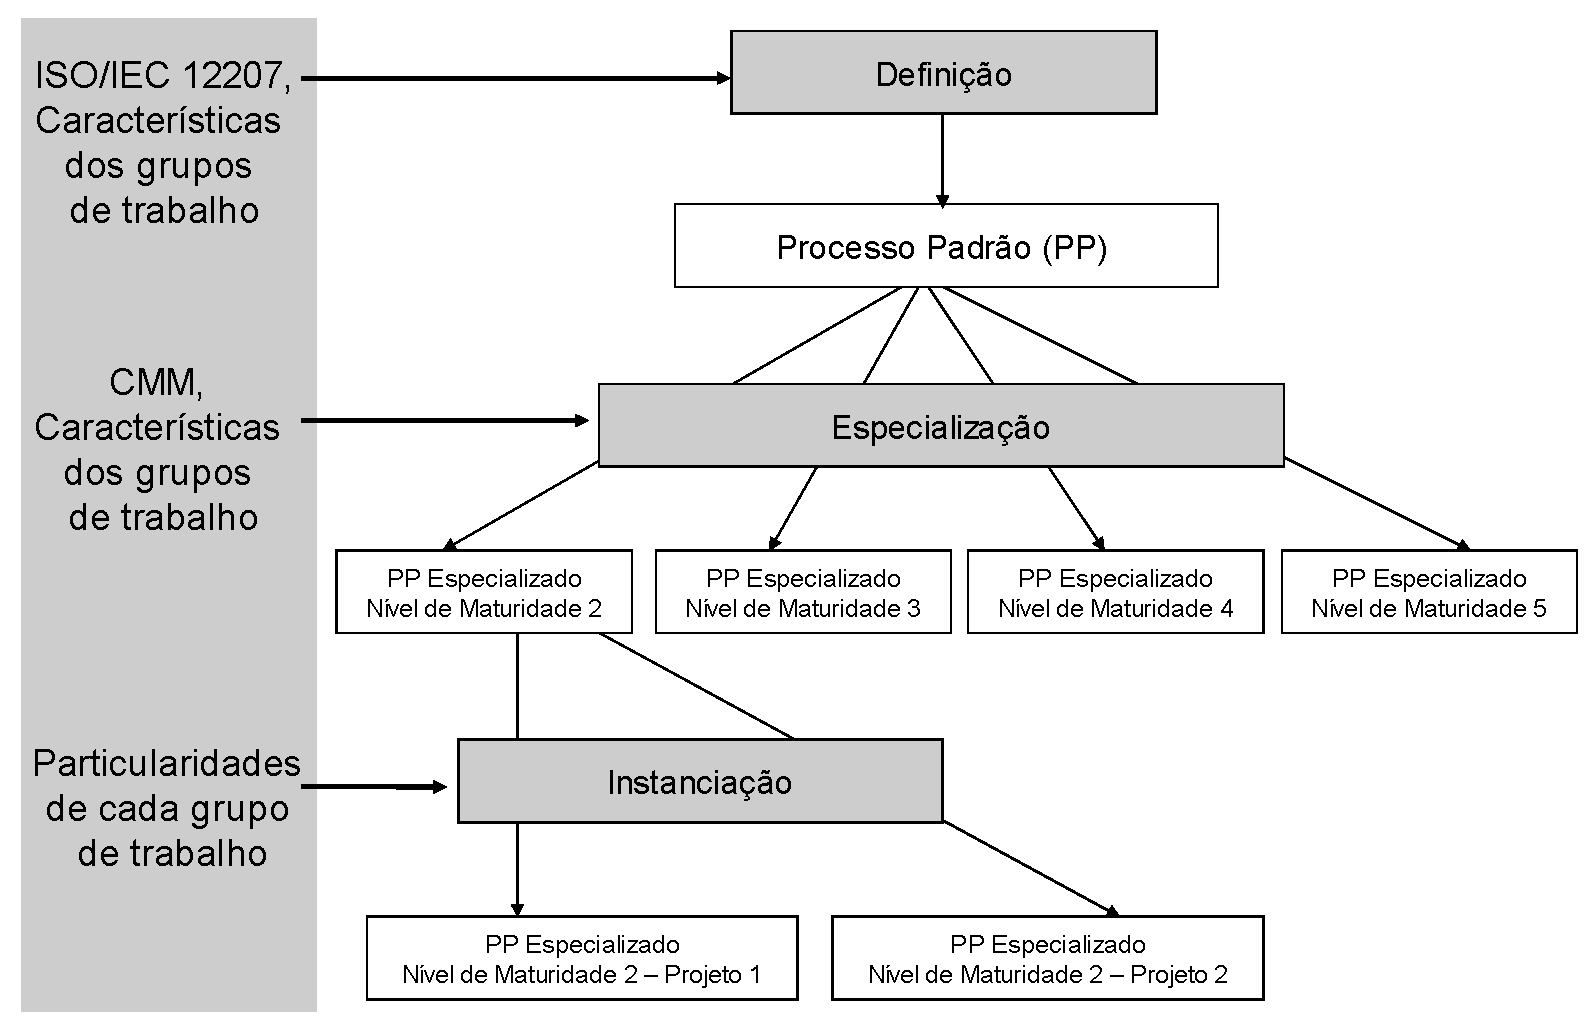
\includegraphics [width=0.85\textwidth]{proposta_maidantchik.pdf}
  \caption{Defini��o de processo de sofware para equipes geograficamente distribu�das \citep{Roc01}}
  \label{proc_mai}
\end{figure}

Neste trabalho, para a defini��o do processo padr�o (Ap�ndice
\ref{pro_padrao}) foram consideradas a norma \cite{ISO12207} e os
objetivos, requisitos, crit�rios e dificuldades discutidos neste
cap�tulo. Para a especializa��o do processo foi considerado o
modelo de maturidade \cite{CMMI2002} (Se��o \ref{especial}). Para a
instancia��o do processo, foi apresentado um exemplo enfatizando a
aloca��o de m�todos, t�cnicas de desenvolvimento, recursos humanos
e tecnol�gicos para as atividades.

\subsection{Estudos de caso: documenta��o, manuten��o e comunica��o}

Os tr�s estudos apresentados a seguir foram realizados no contexto
de disciplinas de cursos de gradua��o do ICMC-USP (estudos de caso
1 e 3) e da Universidade Federal de S�o Carlos (estudo de caso 2).
O objetivo foi observar como os estudantes lidam com determinados
processos, simulando um ambiente de desenvolvimento de pesquisas:
a maioria dos estudantes n�o tinha experi�ncia no dom�nio de
aplica��o proposto e possu�a experi�ncia acad�mica em
desenvolvimento de projetos de software, os trabalhos propostos
foram desenvolvidos em grupos, houve rotatividade de pessoas para
cumprir as tarefas planejadas, ou seja, um grupo iniciava e outro
grupo finalizava as atividades e, em
particular no estudo de caso 3, foi solicitado que simulassem um
ambiente em que os membros da equipe estivessem geograficamente
dispersos e utilizassem alternativas �s reuni�es presenciais para
comunica��o.

A seguir � apresentada uma breve descri��o dos estudos e a
indica��o sobre a utiliza��o dos resultados no processo proposto
neste trabalho.

\subsubsection{Estudo de caso 1: foco na melhoria da documenta��o de projetos de software}

Foi realizado um estudo de caso no segundo semestre de 2002 com o
objetivo de investigar se a abordagem de {\it design rationale}
poderia contribuir para melhorar a documenta��o de projetos de
software. Alguns resultados j� haviam sido apresentados na
literatura, por�m, o foco estava em outras �reas de conhecimento,
por exemplo, Engenharia Mec�nica \citep{Kar96}. O objetivo foi,
portanto, obter ind�cios sobre a aplicabilidade de {\it design
rationale} no contexto de software. Foram investigados dois pontos
principais: 
\begin{enumerate}
\item  se {\it design rationale} contribui para que
engenheiros de software compreendam um projeto anterior; 
\item  se
engenheiros de software est�o interessados em {\it design
rationale} quando precisam compreender um projeto.
\end{enumerate}

Treze estudantes foram divididos em grupos e foi solicitado que
cumprissem determinadas fases de um ciclo de vida de software
tradicional para o desenvolvimento de um projeto, ou seja, an�lise
de requisitos, projeto, projeto de interfaces e testes. Ao mesmo
tempo, foi solicitado que capturassem e registrassem {\it design
rationale} utilizando o modelo IBIS. Os projetos foram trocados
entre os grupos (os temas eram diferentes para cada grupo) e foi
solicitado que implementassem o prot�tipo considerando os
resultados das fases cumpridas anteriormente, por outro grupo.

Foram elaboradas duas quest�es para auxiliar a an�lise dos
resultados. A primeira quest�o foi ``para cada est�gio do ciclo de
vida, as informa��es de {\it design rationale} foram �teis para
auxiliar a compreens�o do projeto?''. Considerando todas as fases
do projeto, foi observado que, em m�dia, {\it design rationale}
foi importante por ajudar a responder 34,99\% das d�vidas dos
estudantes quando eles precisaram compreender o projeto
desenvolvido por outra equipe. Os resultados em rela��o a cada um
dos est�gios do ciclo de vida indicou a utilidade de {\it design
rationale} na compreens�o das fases iniciais do desenvolvimento do
projeto, ou seja, an�lise de requisitos e projeto arquitetural.
Resultados semelhantes foram obtidos para outras �reas de
conhecimento \citep{Kar96} e para o setor industrial
\citep{ConBur1996}.

A segunda quest�o foi ``os engenheiros de software est�o
interessados em {\it design rationale}?''. Foi observada a
frequ�ncia de acesso �s informa��es de {\it design rationale}
pelos grupos. Os resultados obtidos n�o foram conclusivos, pois
nem todos os grupos registraram os dados conforme solicitado, ou
seja, foi registrado apenas que o acesso �s informa��es ocorreu.
Foi observado que todas as informa��es de {\it design rationale}
disponibilizadas foram consultadas. Alguns estudantes mencionaram
a import�ncia em especializar o modelo de {\it design rationale}
para as diferentes fases do ciclo de vida. A descri��o e os
resultados do estudo de caso foram apresentados em
\cite{PaiFor05}.

Os resultados obtidos com a realiza��o deste estudo de caso
indicaram a import�ncia de {\it design rationale} no contexto da
melhoria da documenta��o de software, quando h� rotatividade entre
as pessoas que desenvolve um projeto. Em particular, foram
observados benef�cios quando os artefatos gerados na fase de
an�lise de requisitos precisaram ser compreendidos para que o
desenvolvimento do prot�tipo pudesse ser realizado. Este resultado motivou a realiza��o de
estudos adicionais sobre o uso de {\it design rationale} nas fases
de an�lise de requisitos e projeto de software, com o objetivo de
melhorar a documenta��o obtida. � importante ressaltar que outra
motiva��o foi o resultado apresentado na Figura \ref{gra_corrente}
em rela��o ao processo cumprido atualmente no desenvolvimento de
projetos de pesquisa. Foi observado que as fases de an�lise de
requisitos e projeto est�o entre as tr�s mais valorizadas. Assim,
observou-se que prioriz�-las seria interessante, pois agregaria
valor a uma atividade que � reconhecida pelos pesquisadores e que
apresentou resultados positivos em rela��o ao uso de {\it design
rationale}.

\subsubsection{Estudo de caso 2: foco na import�ncia de {\it design rationale} para manuten��o de software}

Este estudo foi realizado por doze estudantes de p�s gradua��o no segundo semestre de 2003 com o
objetivo de investigar:
\begin{enumerate}
\item  a import�ncia de {\it design
rationale}, resultante de um processo de reengenharia, na
manuten��o de um sistema de software;
\item a import�ncia de {\it design rationale} na redu��o de tempo gasto na manuten��o de
software. Este  segundo item est� relacionado a este trabalho.
\end{enumerate}

Os estudantes foram divididos em 4 grupos e foi proposta uma
atividade de manuten��o em um sistema de oficina eletr�nica,
composta por duas fases. Na primeira fase, foi solicitado que o
sistema permitisse a realiza��o de uma consulta adicional. Na
segunda fase foi solicitada a inclus�o de uma funcionalidade. Para
a realiza��o da primeira manuten��o, os grupos 1 e 2 tiveram
acesso �s informa��es de {\it design rationale} e para a segunda
manuten��o, apenas os grupos 3 e 4 tiveram acesso. Os estudantes
tiveram liberdade para estipular seus hor�rios para desenvolvimento
do trabalho, por�m, foi solicitado que registrassem em um planilha
fornecida o tempo gasto em cada uma das atividades.

Apesar de ser um estudo de caso piloto, foi observado que as
informa��es de {\it design rationale} documentadas durante a
reengenharia do sistema foram importante aux�lio para o
entendimento do projeto durante a realiza��o da atividade de manuten��o. Al�m
disso, o resultado obtido indicou que o tempo gasto na manunten��o
foi menor quando as informa��es de {\it design rationale} estavam
dispon�veis. A descri��o e os resultados do estudo de caso foram apresentados em
\cite{Cagnin04}.

De forma semelhante ao resultado obtido com a realiza��o do estudo
de caso 1, o resultado obtido neste estudo motivou a  realiza��o
de estudos adicionais envolvendo {\it design rationale}, tendo em
vista a melhoria na manuten��o dos projetos.

\subsubsection{Estudo de caso 3: foco na comunica��o entre os participantes do projeto}

Para entender como os estudantes lidam com as quest�es
relacionadas � comunica��o quando um projeto distribu�do �
desenvolvido, foi realizado um estudo de caso no segundo semestre
de 2004 em que o principal objetivo era tornar expl�citas as
caracter�sticas do processo da comunica��o, que � um requisito dos
usu�rios do processo proposto.

Como atividade proposta, foi solicitado que estudantes de duas
turmas da disciplina de Engenharia de Software do ICMC-USP (94
estudantes no total) realizassem determinadas altera��es
(pr�-definidas) em c�digo fonte desenvolvido por estudantes de
outra disciplina, utilizando ferramentas de software livre para
apoiar a comunica��o e simulando um ambiente de desenvolvimento
distribu�do de software. Os estudantes foram incentivados a
desenvolver os projetos de forma colaborativa, dividindo tarefas e
registrando d�vidas, coment�rios e decis�es tomadas, sem realizar
encontros presenciais. Eles estavam matriculados em dois cursos
diferentes e os grupos foram formados por estudantes de turmas
diferentes.

Como resultados obtidos, em resumo, pode-se destacar:
\begin{enumerate}
\item no in�cio do desenvolvimento do projeto foi notada a resist�ncia dos estudantes em rela��o ao estabelecimento inicial da comunica��o, o que indicou a necessidade de refor�ar o treinamento (em termos te�ricos e pr�ticos) e motivar a equipe em rela��o � comunica��o; 
\item  quando as d�vidas em rela��o � resolu��o do problema come�aram a surgir, a comunica��o foi intensificada e aos poucos se tornou mais natural;
\item os estudantes se empenharam em conhecer novas ferramentas que auxiliassem a comunica��o e a vencer as dificuldades que surgem quando a distribui��o geogr�fica � uma caracter�stica do desenvolvimento. 
\end{enumerate}

A descri��o e os resultados do estudo de caso foram apresentados em \cite{Paiva05}. Os resultados obtidos foram positivos no sentido de indicar que �
poss�vel vencer as limita��es do ambiente de desenvolvimento de
pesquisas, como a escassez de recursos, quando h� motiva��o dos
estudantes em rela��o � comunica��o e ao desenvolvimento
distribu�do. A import�ncia do treinamento tamb�m foi refor�ada. %Al�m disso, foram indicadas vantagens e desvantagens
%de ferramentas que auxiliam na comunica��o, enfatizadas na Se��o X
%(parte de instancia��o).


\subsection{Estudo de caso: avalia��o e melhoria do processo}

O projeto {\it No-Risk Planning} foi iniciado em 2001 por um estudante do curso gradua��o em Ci�ncia da Computa��o do ICMC-USP como projeto de fim de curso \citep{moura01}. O objetivo foi desenvolver um sistema de agenda que estivesse dispon�vel na {\it web} e permitisse o agendamento de compromissos de grupos de trabalho. Durante o desenvolvimento do prot�tipo inicial, apenas o c�digo fonte e o modelo l�gico da base de dados foram disponibilizados.

Tendo em vista as dificuldades enfrentadas por dois estudantes (um aluno de inicia��o cient�fica e um de mestrado) em dar continuidade ao desenvolvimento do projeto \citep{Rib2003}, decidiu-se por dar �nfase ao processo de desenvolvimento utilizado. Dessa forma, em paralelo � evolu��o das funcionalidades do software, iniciavam-se as atividades de melhoria do processo de desenvolvimento do sistema. O modelo IDEAL \citep{GreMye97} e a norma \cite{ISO12207} foram utilizados para guiar o cumprimento das atividades de melhoria do processo \citep{PaiSanFor2003}.

Em uma primeira iniciativa, foram priorizadas, basicamente,
atividades de ciclo de vida (processos fundamentais), atividades
de ger�ncia (processos organizacionais) e atividades de ger�ncia
de configura��o (processos de apoio). Em rela��o aos processos
fundamentais, foram propostas melhorias na execu��o das atividades
de especifica��o de requisitos, an�lise do sistema, projeto
navegacional do sistema, realiza��o de testes de unidade e de
aceita��o. Para os processos organizacionais foram considerados o
gerenciamento de prazos e de recursos. As atividades relacionadas
aos processos de apoio foram o controle de vers�es e a garantia da
conclus�o, consist�ncia e corre��o dos itens. A equipe respons�vel
pelo projeto se empenhou em cumprir as atividades priorizadas e,
como resultado, um processo de desenvolvimento de software inicial
foi estabelecido e a documenta��o do sistema foi notoriamente
melhorada \citep{ribeiro:03}.

A partir do uso expressivo do sistema por usu�rios finais,
conforme apresentado por \cite{Frei04}, diversos requisitos novos
surgiram e notou-se que a implementa��o eficiente desses
requisitos exigia mais melhorias em termos de documenta��o e
melhor controle (gerenciamento) do processo de desenvolvimento.
Dessa forma, processos especializados para desenvolvimento de
software para ambiente {\it web} foram investigados, tendo sido adotada
a proposta elaborada por \cite{pres01}, que prop�e que sejam
cumpridas as atividades de formula��o e planejamento, an�lise,
engenharia, gera��o de testes e avalia��o com usu�rios; al�m de
considerar princ�pios de gerenciamento. Com a ado��o dessa
abordagem foi poss�vel considerar no processo elementos
caracter�sticos de um desenvolvimento voltado para o ambiente {\it web},
por exemplo, a evolu��o cont�nua das aplica��es e o planejamento
de interfaces considerando elementos do contexto {\it web}
\citep{For04}.

� importante destacar tamb�m que o desenvolvimento do projeto {\it
No-Risk Planning} passou a ser realizado utilizando o conjunto de
ferramentas oferecidas pela Incubadora Virtual da Fapesp, ou seja,
foram utilizadas ferramentas para apoio �s atividades de controle
de vers�es, controle de bugs, gerenciamento de tarefas,
requisi��es de novas funcionalidades, gerenciamento de
documenta��o, listas de discuss�o, f�runs, entre outros. A
utiliza��o dessas ferramentas tamb�m contribuiu para a melhoria do
processo. Outras informa��es sobre a realiza��o do estudo de caso
podem ser encontradas em \cite{pfsf04a}.

A experi�ncia adquirida com a realiza��o deste estudo de caso foi
importante principalmente em rela��o � forma de implanta��o do
processo, ou seja, foi observada na pr�tica a import�ncia em
propor a melhoria gradual de um processo e em
considerar elementos do dom�nio e do tipo de aplica��o
desenvolvido para que os esfor�os de melhoria sejam bem sucedidos.
Al�m disso, os resultados obtidos com o uso de ferramentas que
ap�iam o desenvolvimento de projetos distribu�dos em ambiente de
pesquisa foram considerados.

As etapas seguintes da proposta de Humphrey para defini��o de
processos se referem � defini��o e valida��o do processo. Os
resultados obtidos com a execu��o destas etapas s�o apresentados
no Cap�tulo \ref{proc_pes}.


\section {Considera��es finais}

Neste cap�tulo foram apresentadas as atividades cumpridas para a concep��o de um processo para o desenvolvimento de projetos de pesquisa. A abordagem proposta por \cite{Hum95} para a defini��o de processos de software foi utilizada. O principal benef�cio obtido foi a possibilidade de tomar consci�ncia e refletir sobre diversos elementos fundamentais da defini��o de um processo. Provavelmente a import�ncia desses elementos n�o teria sido observada se uma abordagem sistem�tica n�o tivesse sido utilizada.

Em particular, duas limita��es podem ser destacadas em rela��o �
concep��o do processo apresentada neste cap�tulo. A primeira se
refere � fase de defini��o de objetivos e metas. De acordo com a
proposta de Humphrey, nesta fase devem ser definidas m�tricas e os
resultados esperados devem ser indicados. Na Se��o \ref{obj} foi
discutido um conjunto restrito de m�tricas e, al�m disso, n�o
foram encontrados dados hist�ricos e estimativas de projetos
anteriores que pudessem auxiliar na proposi��o de resultados
esperados.

Outra limita��o est� relacionada � estrat�gia de desenvolvimento
do processo. Humphrey sugere que esta etapa seja fortemente
baseada em observa��o. Alguns estudos de caso foram realizados
sendo que foi solicitado aos estudantes que cumprissem as tarefas
pr�-determinadas. N�o foi considerado se havia motiva��o para
desempenhar a tarefa e como eles iriam proceder se pudessem escolher a
forma de desempenh�-la.


\chapter{Processo para Projetos de Pesquisa em Software} \label{proc_pes}

\section{Considera��es iniciais}

Neste cap�tulo � apresentado o processo proposto para desenvolvimento de projetos de pesquisa em software. Ap�s uma breve discuss�o, em que s�o retomados os principais elementos que foram importantes para a defini��o do processo, � apresentado o processo padr�o. Em seguida s�o apresentados o processo especializado e um exemplo de instancia��o da proposta. O modelo CMMI foi utilizado para apoiar a etapa de especializa��o e a instancia��o foi realizada no contexto do desenvolvimento do projeto SAFE ({\it Software Engineering Available for Everyone}). Por fim, s�o discutidos tamb�m aspectos da avalia��o do processo. 

\section{Fundamentos para a elabora��o do processo proposto} \label{funda}

Para a defini��o do processo padr�o foram considerados aspectos
espec�ficos do desenvolvimento de projetos distribu�dos e
colaborativos e do desenvolvimento de software livre. Al�m disso,
conforme sugerido na literatura, buscou-se combinar elementos de
metodologias �geis e de metodologias tradicionais. � importante destacar tamb�m os
processos que tornam vi�veis o estabelecimento de parcerias entre
universidades e empresas.

� poss�vel notar, como caracter�sticas semelhantes entre o
desenvolvimento de projetos de software livre e o desenvolvimento
de projetos de pesquisa, a evolu��o cont�nua do projeto, em que
novas vers�es s�o frequentemente disponibilizadas; a aus�ncia de um
conjunto determinado de requisitos no in�cio do desenvolvimento do
projeto; a dispers�o geogr�fica dos membros e a
distribui��o gratuita do software desenvolvido em grande parte dos
projetos. Em especial, as experi�ncias e as pr�ticas cumpridas
pela comunidade de software livre contribu�ram para a defini��o dos processos de coordena��o, de comunica��o
e de gerenciamento.

O desenvolvimento distribu�do e colaborativo � uma das principais
caracter�sticas do desenvolvimento de projetos de pesquisa. Assim,
em particular, pr�ticas indicadas por \cite{mai99} na proposta de
um processo para o desenvolvimento de projetos distribu�dos e por
\cite{hum99}, na proposta de um processo para desenvolvimento de
projetos por equipes, foram enfatizadas. De forma geral,
conforme apresentado no Cap�tulo \ref{processo_software},
processos importantes neste contexto se referem ao gerenciamento
de configura��o, comunica��o, gerenciamento e coordena��o de
projetos, estabelecimento da infra-estrutura, gerenciamento
de requisitos, planejamento e controle de projetos e garantia da
qualidade.

Dois importantes valores defendidos nas propostas de m�todos �geis
para desenvolvimento de software foram considerados no contexto
deste trabalho. Em um dos valores � enfatizado que software
funcional � mais importante que documenta��o detalhada. Foi
observado, conforme apresentado no Cap�tulo \ref{cap_concepcao}, que em geral h�
pouca experi�ncia com o cumprimento de boas pr�ticas para
desenvolvimento de projetos de pesquisa. Conforme sugerido por
\cite{Hum95}, propor uma mudan�a dr�stica nos processos cumpridos
correntemente n�o � vi�vel. Assim, considerando este valor, foi
proposto uma documenta��o simplificada das atividades a serem
cumpridas, por�m, incluindo elementos essenciais.

Outro valor importante considerado na proposta de m�todos �geis
est� relacionado a priorizar a resposta a mudan�as, ao inv�s do
cumprimento de um plano. Trazendo para o contexto do
desenvolvimento de pesquisas, nota-se que tamb�m h� a prioridade
em investigar respostas para as quest�es de pesquisa quando elas surgem.  Assim, a obten��o
de conhecimento, a proposta de solu��es inovadoras e as
investiga��es para a resolu��o dos problemas de pesquisa tamb�m
devem ser considerados como primordiais.

Conforme observado por \cite{Jen04} e \cite{Mac96}, � dif�cil
implementar a parceria entre academia e ind�stria por diversos
motivos, dentre eles, a falta de interesse de membros da academia
em projetar sistemas para a �rea de neg�cios e em elaborar
materiais apropriados para oferecer treinamento para a ind�stria. No entanto, apesar das dificuldades, membros da academia, da
ind�stria e do governo t�m buscado desenvolver projetos
conjuntamente e, sobretudo, aprender com os erros, propor modelos
de parceria, estender seus dom�nios e melhorar seus neg�cios e
suas pesquisas de acordo com as experi�ncias obtidas.

Diversos autores, baseados em suas experi�ncias, indicaram
atividades consideradas fundamentais para que a parceria entre
universidade e ind�stria aconte�a. \cite{Korn03} destacaram a
import�ncia em definir claramente objetivos, pap�is e
responsabilidades, usar uma abordagem incremental para o
desenvolvimento de software, elaborar documenta��o completa dos
projetos, incluindo elementos de {\it design rationale}.
\cite{Jen04} destaca a import�ncia do gerenciamento efetivo do
projeto. \cite{Mac96} indicaram tamb�m a import�ncia da defini��o
clara de objetivos e pap�is e destacaram a import�ncia da forma��o de
equipes cujos membros se comunicam com facilidade, da divis�o do projeto em
fases, do uso de um processo iterativo, da compatibilidade entre os
treinamentos oferecidos e dos interesses das entidades envolvidas.

Em ambiente de desenvolvimento de pesquisas observa-se que os requisitos s�o
identificados primordialmente de forma iterativa \citep{seg05}.
Al�m disso, h� interesse no desenvolvimento de prot�tipos, com o
objetivo de validar resultados de pesquisa. Estes prot�tipos
geralmente s�o continuados por diversos estudantes e pesquisadores
e, conforme observado por \cite{Bol04}, �
fundamental produzir documenta��o que contribua para
garantir a evolu��o das investiga��es e a obten��o de resultados
cient�ficos.

%Conforme apresentado por \cite{paa04}, quando um projeto � desenvolvido de forma distribu�da, n�o �
%necess�rio que as equipes envolvidas adotem o mesmo processo.
%Quando estas equipes cumprem algum processo considerado
%satisfat�rio, deve ocorrer apenas a sincroniza��o entre as
%principais fases do processo e os {\it milestones}. Sugere-se,
%ainda, que seja utilizado um modelo de processo incremental e os
%participantes devem sincronizar os ciclos de itera��o, isto �,
%eles devem ter o mesmo tamanho.

%Os processos de engenharia englobam o m�todo da prototipa��o,
%pr�ticas de desenvolvimento �gil e o registro de design rationale.
%Conforme apresentado na Figura \ref{eng}, sugere-se que o
%desenvolvimento ocorra de forma iterativa, (incremental?? ver
%termos usados no artigo do seg05 e no livro do praxis),
%disponibilizando-se releases com a maior frequ�ncia poss�vel. Na
%�ltima itera��o disponibiliza-se o prot�tipo.

%{\bf Vis�o geral do subprocesso:} engloba atividades de um desenvolvimento �gil consideradas em um contexto de prototipa��o. Tradicionalmente, prot�tipos s�o constru�dos para ajudar o projetista a refinar os requisitos do sistema. Geralmente � constru�do um software simples, sem documenta��o, pouco eficiente. Em ambiente acad�mico geralmente s�o desenvolvidos prot�tipos (como resultado das pesquisas realizadas) que s�o continuados por diversos estudantes e pesquisadores. Neste processo enfatiza-se a utiliza��o das principais fases da prototipa��o considerando-se pr�ticas de desenvolvimento �gil, de forma que uma documenta��o elementar seja gerada. (Pressman fala na pagina 75 sobre uso de prototipa��o junto com m�todos ageis).

%O desenvolvimento de prot�tipos, ao inv�s de produtos, � uma caracter�stica do ambiente acad�mico. S�o consideradas, basicamente, as atividades propostas pelo m�todo da prototipa��o. Em ambiente acad�mico, nem sempre � simples definir o tema do projeto que ser� desenvolvido \cite{DuSoBuRe04a} e, portanto, uma atividade relacionada foi inclu�da

%OBS: Pg 77 - Pressman: Fuzzy problem solving ability: H� uma relacao entre DR e metodos ageis. H� um link entre metodos ageis, prototipa��o e li��es aprendidas.


\section{Processo padr�o para desenvolvimento de projetos de pesquisa em software}

Na Figura \ref{fig1} � apresentada uma vis�o geral do processo padr�o para o desenvolvimento de projetos de pesquisa em software. Processos apresentados em caixas com fundo branco s�o equivalentes a processos apresentados na norma e processos apresentados em caixas com fundo cinza foram inclu�dos como resultado da realiza��o deste trabalho.

\begin{figure} [!ht]
 \centering
  \bfseries
  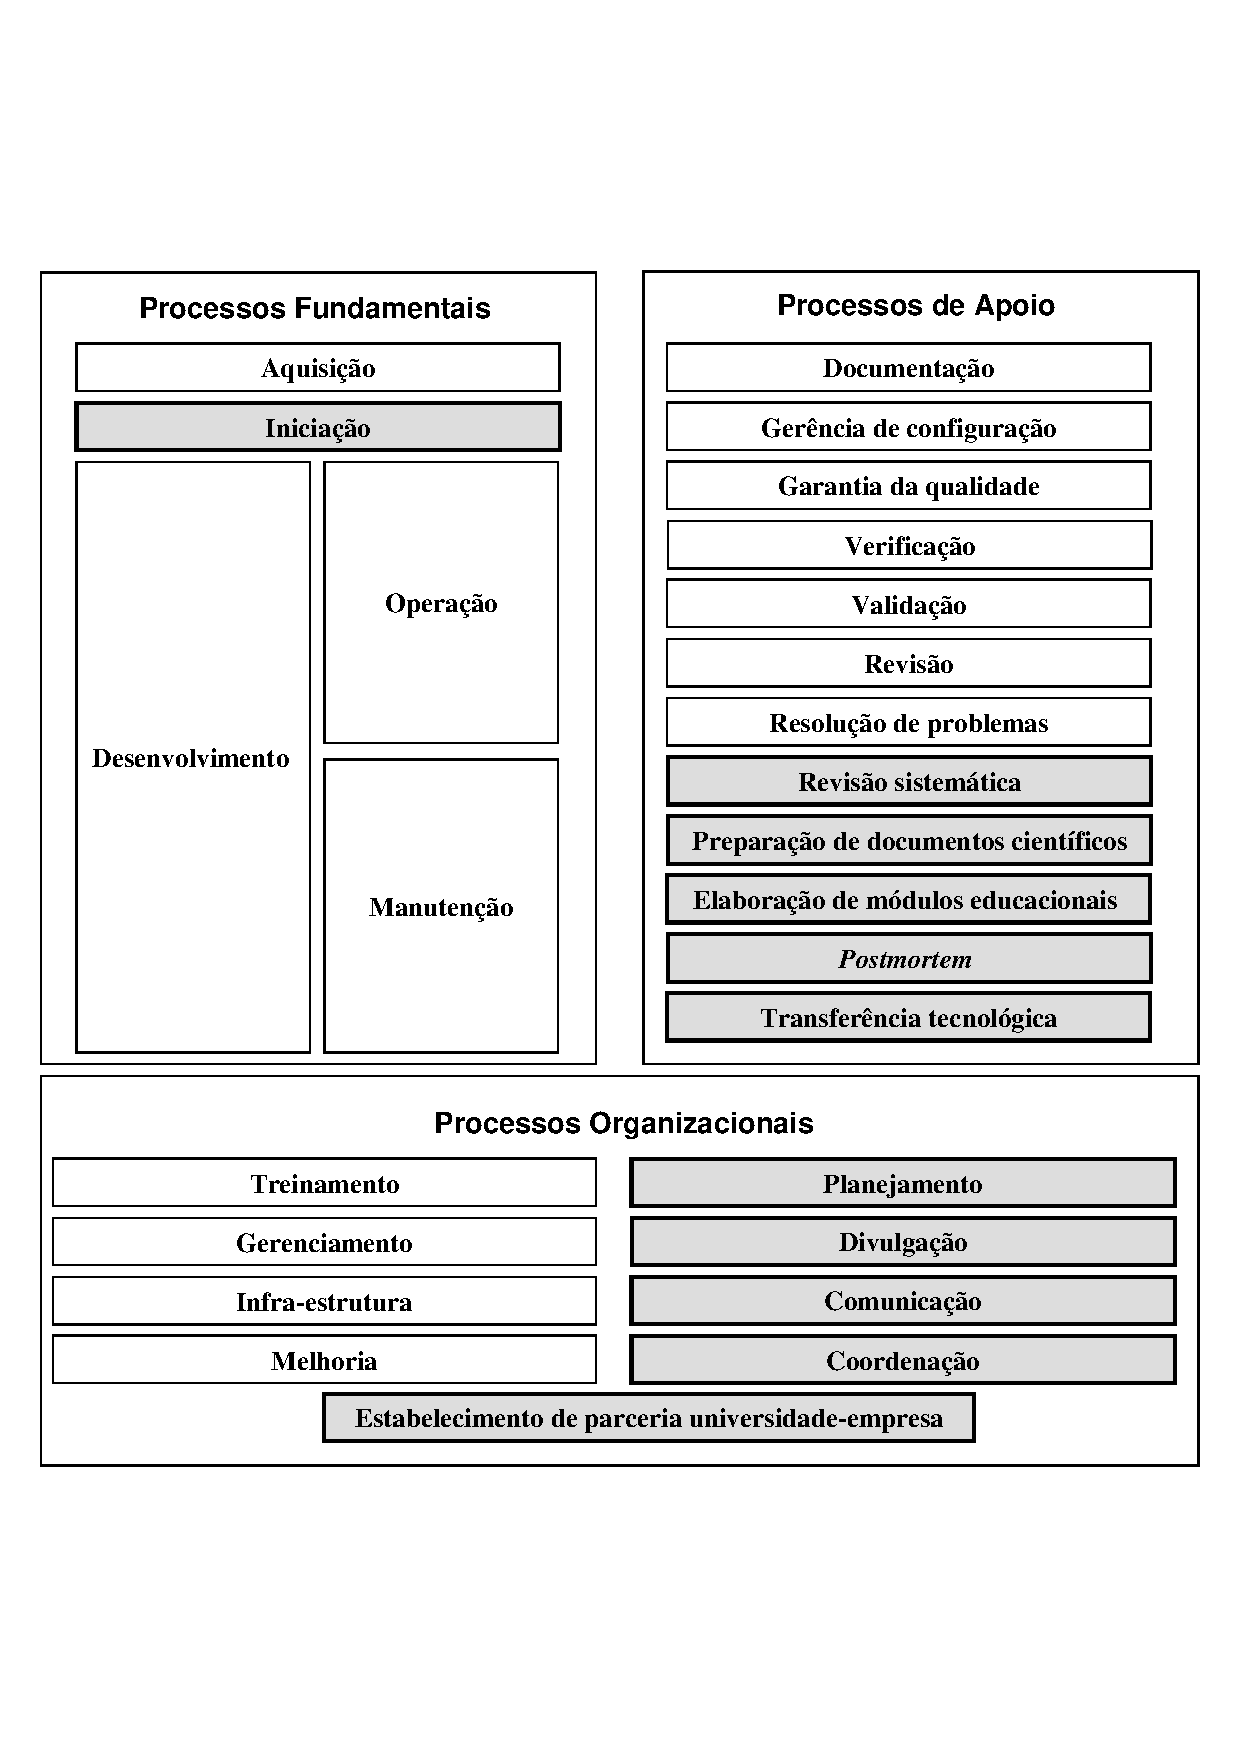
\includegraphics [width=0.95\textwidth]{Processo_Padrao.pdf}
  \caption {Processo padr�o para o desenvolvimento de projetos de pesquisa}
  \label{fig1}
\end{figure}

%As principais diferen�as entre a norma ISO/IEC 12207 e o processo para desenvolvimento de projetos de pesquisa em rela��o aos processos fundamentais s�o:

%\begin{itemize}

%\item O processo ``Fornecimento'', presente na norma ISO/IEC 12207, n�o foi inclu�do no processo para desenvolvimento de projetos de pesquisa. Foi observado, no entanto, que atividades referentes ao processo ``Estabelecimento de Parceria Universidade-Empresa'' (inclu�do neste trabalho) est�o relacionados ao processo proposto na norma. 

%\item O processo ``Inicia��o'' foi inclu�do com o objetivo de englobar atividades de prepara��o para desenvolvimento de projetos de pesquisa. %como escolha do tema do projeto de pesquisa e elabora��o de um plano de pesquisa.

%\end{itemize}

%As principais diferen�as entre a norma ISO/IEC 12207 e o processo para desenvolvimento de projetos de pesquisa em rela��o aos processos de apoio s�o:

%\begin{itemize}

%\item O processo ``Auditoria''\footnote{Na norma ISO/IEC 12207, no processo de auditoria � avaliada a conformidade a requisitos, planos e contratos}, presente na norma ISO/IEC 12207, n�o foi inclu�do no processo para desenvolvimento de projetos de pesquisa porque, conforme indicado na Se��o \ref{funda}, foi priorizado respostas a mudan�as, ao inv�s do cumprimento de planos. � poss�vel, no entato, que tal processo seja importante quando h� parcerias entre universidades e empresas. N�o foram encontrados relatos na literatura indicando a import�ncia e as atividades relacionadas ao processo neste caso e, assim, optou-se pela n�o inclus�o do processo. 

%\item O processo ``Revis�o Sistem�tica'' foi inclu�do, apesar de n�o haver sido mencionado pelos usu�rios do processo. A inclus�o ocorreu devido a observa��o da import�ncia deste processo durante o desenvolvimento de projetos de pesquisa.

%\item O processo ``{\it Postmortem}'' foi inclu�do por ter sido mencionado como um requisito dos usu�rios e por fornecer uma alternativa (bastante valorizada na literatura) para obten��o de conhecimento sobre os projetos. Esse conhecimento pode contribuir para a melhoria na forma como os projetos subjacentes ser�o desenvolvidos. 


%\item Os processos ``Prepara��o de documentos cient�ficos'', ``Elabora��o de m�dulos educacionais'' e ``Transfer�ncia tcnol�gica'' foram inclu�dos por serem requisitos dos usu�rios.

%\end{itemize}

%As principais diferen�as entre a norma ISO/IEC 12207 e o processo para desenvolvimento de projetos de pesquisa em rela��o aos processos organizacionais se refere � inclus�o dos processos de ``Planejamento'', ``Divulga��o'', ``Comunica��o'', ``Coordena��o'' e ``Estabelecimento de parceria universidade-empresa'', que foram requisitos dos usu�rios.

A descri��o dos processos considerando-se o contexto de
desenvolvimento de projetos de pesquisa � apresentada no Ap�ndice
2. Conforme indicado no Cap�tulo \ref{processo_software}, �
fundamental apresentar {\it guidelines} que auxiliem a execu��o do
processo, incluindo, por exemplo, atividades e artefatos a serem
produzidos. 

Para a descri��o do processo padr�o, foi utilizada uma estrutura
semelhante �quela apresentada na norma IS0/IEC 15504, parte 5. Portanto, neste trabalho, para cada processo s�o descritas suas atividades sendo que para cada atividade s�o apresentados (a) identificador, (b) proposta, (c) resultados e (d) tarefas. Para cada tarefa s�o apresentados (a) objetivos, (b) artefatos de entrada e (c) artefatos de sa�da.  

 
\section{Especializa��o do processo padr�o para projetos de pesquisa em software} \label{especial}

De acordo com a proposta apresentada por \cite{mai99}, o processo padr�o deve ser especializado
de forma a indicar uma abstra��o espec�fica para um determinado
contexto. A principal motiva��o para a especializa��o do processo padr�o � permitir que gerentes e coordenadores
de equipes abstraiam determinados aspectos do processo com o objetivo de atender as �reas de um dado n�vel de maturidade. Dessa forma, a especializa��o requer que seja estabelecida a correspond�ncia entre os diferentes aspectos do processo padr�o e as �reas apresentadas no modelo de maturidade. Assim, � poss�vel identificar os aspectos do
processo os quais devem ser enfatizados a fim de atender �s �reas de um determinado n�vel
de maturidade. 

Neste trabalho, com o objetivo de atender �s diferentes
caracter�sticas das equipes que participam do desenvolvimento de
projetos de pesquisa, foi realizada a especializa��o do processo
padr�o de forma a permitir que cada equipe utilize um processo com
n�vel de maturidade compat�vel � sua capacidade. Para especializar
o processo foi estabelecido como refer�ncia o modelo CMMI \citep{CMMI2002} (representa��o por est�gios), no qual
foram definidos os diferentes n�veis de maturidade de um processo. Os resultados obtidos s�o apresentados na Tabela \ref{epc} (para especializa��o em rela��o ao n�vel 2 do CMMI) e na Tabela \ref{nivel3} (para especializa��o em rela��o ao n�vel 3 do CMMI). Foi observado que para os n�veis 4 e 5 do CMMI n�o h� processos correspondentes no processo padr�o elaborado. Conforme apresentado no Cap�tulo \ref{acabou}, o estudo da viabilidade da inclus�o dos processos referentes a estes n�veis � um dos trabalhos futuros propostos.  

% %\begin{tabular}{|l|l|l|l|}
\begin{table}[!ht]
\begin{center}
\caption{Especializa��o do processo padr�o para o n�vel 2 do CMMI}\label{epc}
\begin{tabular}{|p{3.5cm}|p{4cm}|p{2.5cm}|p{3cm}|}
\hline
{\bf \small �reas de processo do CMMI (n�vel 2)} & {\bf \small Processo padr�o para desenvolvimento de projetos de pesquisa em software} & {\bf \small Atividades do processo padr�o} & {\bf \small Tarefas do processo padr�o} \\ 
\hline
\small Gerenciamento de requisitos & \small Gerenciamento & \small GN & \small GN.1 \\ 
\hline
\small Planejamento de projeto & \small Planejamento  & \small DE, PI, PZ, PC, PS & \small DE.1, DE.2, PI.1, PI.2, PI.3, PZ.1, PC.1, PS.1, PS.2, PS.3 \\ 
\cline{2-4}
 & \small Inicia��o & \small ET, EP & \small ET.1, ET.2, ET.3, ET.4, EP.1, EP.2 \\ 
\cline{2-4}
 & \small Documenta��o & \small PD & \small PD.1 \\ 
\cline{2-4}
 & \small Infra-estrutura & \small IT, IF & \small IT.1, IT.2, IF.1 \\ 
\hline
\small Monitoramento e controle de projeto & \small Coordena��o & \small MR, EC & \small MR.1, EC.1 \\ 
\hline
\multicolumn{1}{|c|}{--} & \small Aquisi��o & \small AQ, AR & \small AQ.1, AQ.2, AR.1, AR.2, AR.3 \\ 
\hline
\small Ger�ncia de subcontrata��o & \small Estabelecimento de parceria universidade-empresa & \small EA & \small EA.1, EA.2, EA.3 \\ 
\hline
\small Medi��o e an�lise & \multicolumn{1}{c|}{--} & \multicolumn{1}{c|}{--} & \multicolumn{1}{c|}{--} \\ 
\hline
\small Garantia de qualidade de processo e de produto & \small Garantia da qualidade & \small IC, GQ, GA & \small IC.1, GQ.1, GA.1 \\ 
\cline{2-4}
 & \small Documenta��o  & \small IP, PO & \small IP.1, PO.1 \\ 
\cline{2-4}
 & \small Revis�o & \small IB, RR & \small IB.1, RR.1, RR.2, RR.3 \\ 
\cline{2-4}
 & \small Resolu��o de problemas & \small ID, RP & \small ID.1, RP.1 \\ 
\hline
\small Gerenciamento de configura��o & \small Ger�ncia de configura��o & \small IO, II, CC, AC & \small IO.1, II.1, CC.1, CC.2, CC.3, AC.1 \\ 
\hline
\multicolumn{1}{|c|}{--} & \small Revis�o sistem�tica & \small IM, RE & \small IM.1, RE.1, RE.2, RE.3 \\ 
\hline
\multicolumn{1}{|c|}{--} & \small Prepara��o de documentos cient�ficos & \small RD, FD & \small RD.1, FD.1 \\ 
\hline
\multicolumn{1}{|c|}{--} & \small Elabora��o de m�dulos educacionais & \small EM  & \small EM.1, EM.2, EM.3 \\ 
\hline
\multicolumn{1}{|c|}{--} & \small Divulga��o & \small IA, DI & \small IA.1, DI.1, DI.2 \\ 
\hline
\multicolumn{1}{|c|}{--} & \small Comunica��o & \small IN, PC & \small IN.1, PC.1, PC.2 \\ 
\hline
\end{tabular}
\end{center}
\end{table}

\begin{table}[!ht]
\begin{center}
\caption{Especializa��o do processo padr�o para o n�vel 2 do CMMI.  \small No Ap�ndice B desta tese encontram-se as descri��es das atividades e tarefas que est�o apresentadas nesta tabela por meio de seus identificadores.}\label{epc}
\begin{tabular}{|p{3.8cm}|p{4cm}|p{2.5cm}|p{2.8cm}|}
\hline
\bf \footnotesize \centering Modelo CMMI \\ \centering (n�vel 2) & 
\multicolumn{3}{|c|}{\textbf{\footnotesize Processo Padr�o para Projetos de Pesquisa em Software}}\\
\hline
\bf \footnotesize  �reas &
\bf \footnotesize  Processos &
\bf \footnotesize  Atividades  &
\bf \footnotesize Tarefas\\  
\hline
\footnotesize Gerenciamento de re\-quisitos & \footnotesize \sffamily Gerenciamento & \footnotesize  GN & \footnotesize  GN.1 \\ 
\hline
\footnotesize Planejamento de projeto & \footnotesize \sffamily Planejamento  & \footnotesize   DE, PI, PZ, PC, PS & \footnotesize  DE.1, DE.2, PI.1, PI.2, PI.3, PZ.1, PC.1, PS.1, PS.2, PS.3 \\ 
\cline{2-4}
 & \footnotesize \sffamily Inicia��o & \footnotesize  ET, EP & \footnotesize  ET.1, ET.2, ET.3, ET.4, EP.1, EP.2 \\ 
\cline{2-4}
 & \footnotesize \sffamily Documenta��o & \footnotesize  PD & \footnotesize  PD.1 \\ 
\cline{2-4}
 & \footnotesize \sffamily Infra-estrutura & \footnotesize IT, IF & \footnotesize IT.1, IT.2, IF.1 \\ 
\hline
\footnotesize  Monitoramento e con\-trole de projeto & \footnotesize \sffamily Coordena��o & \footnotesize MR, EC & \footnotesize MR.1, EC.1 \\ 
\hline
\multicolumn{1}{|c|}{--} & \footnotesize \sffamily Aquisi��o & \footnotesize AQ, AR & \footnotesize AQ.1, AQ.2, AR.1, AR.2, AR.3 \\ 
\hline
\footnotesize Ger�ncia de subcontrata��o & \footnotesize \sffamily Estabelecimento de parceria universidade-empresa & \footnotesize EA & \footnotesize EA.1, EA.2, EA.3 \\ 
\hline
\footnotesize Medi��o e an�lise & \multicolumn{1}{c|}{--} & \multicolumn{1}{c|}{--} & \multicolumn{1}{c|}{--} \\ 
\hline
\footnotesize Garantia de qualidade de processo e de produto & \footnotesize \sffamily Garantia da qualidade & \footnotesize IC, GQ, GA & \footnotesize IC.1, GQ.1, GA.1 \\ 
\cline{2-4}
 & \footnotesize \sffamily Documenta��o  & \footnotesize IP, PO & \footnotesize IP.1, PO.1 \\ 
\cline{2-4}
 & \footnotesize \sffamily Revis�o & \footnotesize IB, RR & \footnotesize IB.1, RR.1, RR.2, RR.3 \\ 
\cline{2-4}
 & \footnotesize \sffamily Resolu��o de problemas & \footnotesize ID, RP & \footnotesize ID.1, RP.1 \\ 
\hline
\footnotesize Gerenciamento de configura��o & \footnotesize \sffamily Ger�ncia de configura��o & \footnotesize IO, II, CC, AC & \footnotesize IO.1, II.1, CC.1, CC.2, CC.3, AC.1 \\ 
\hline
\multicolumn{1}{|c|}{--} & \footnotesize \sffamily Revis�o sistem�tica & \footnotesize IM, RE & \footnotesize IM.1, RE.1, RE.2, RE.3 \\ 
\hline
\multicolumn{1}{|c|}{--} & \footnotesize \sffamily Prepara��o de documentos cient�ficos & \footnotesize RD, FD & \footnotesize RD.1, FD.1 \\ 
\hline
\multicolumn{1}{|c|}{--} & \footnotesize \sffamily Elabora��o de m�dulos edu\-ca\-cionais & \footnotesize EM  & \footnotesize EM.1, EM.2, EM.3 \\ 
\hline
\multicolumn{1}{|c|}{--} & \footnotesize \sffamily Divulga��o & \footnotesize IA, DI & \footnotesize IA.1, DI.1, DI.2 \\ 
\hline
\multicolumn{1}{|c|}{--} & \footnotesize \sffamily Comunica��o & \footnotesize IN, PC & \footnotesize IN.1, PC.1, PC.2 \\ 
\hline
\end{tabular}
\end{center}
\end{table}



%\begin{table}[!ht]
\begin{center}
\caption{Especializa��o do processo padr�o para o n�vel 3 do CMMI}\label{nivel3}
\begin{tabular}{|p{3.5cm}|p{4cm}|p{2.5cm}|p{3cm}|}
\hline{\bf �reas de processo do CMMI (n�vel 3)} & {\bf Processo padr�o para desenvolvimento de projetos de pesquisa em software} & {\bf Atividades do processo padr�o} & {\bf Tarefas do processo padr�o} \\ 
\hline
Desenvolvimento de requisitos & Inicia��o & AE & AE.1, AE.2  \\ 
\cline{2-4}
 & Desenvolvimento & DF  & DF.1 \\ 
\hline
Solu��o t�cnica & Inicia��o  & PA  & PA.1 \\ 
\cline{2-4}
 & Desenvolvimento & PR, PP, DP, AP & PR.1, PP.1, DP.1, DP.2, DP.3, AP.1, AP.2, AP.3 \\ 
\cline{2-4}
 & Opera��o & GU, SU & GU.1, SU.1 \\ 
\cline{2-4}
 & Manuten��o  & PM, RM & PM.1, RM.1, RM.2, RM.3, RM.4 \\ 
\hline
Integra��o do produto  & Desenvolvimento & IR  & IR.1, IR.2, IR.3 \\ 
\hline
Verifica��o  & Verifica��o  & IE, VE & IE.1, VE.1 \\ 
\hline
Valida��o & Valida��o & IS, VA & IS.1, VA.1 \\ 
\hline
Foco no processo organizacional & Melhoria  & DR, AO, MP & DR.1, AO.1, AO.2, MP.1, MP.2 \\ 
\hline
Defini��o do processo da organiza��o & \multicolumn{1}{c|}{--} & \multicolumn{1}{c|}{--} & \multicolumn{1}{c|}{--} \\ 
\hline
Treinamento organizacional & Treinamento  & IL, TR & IL.1, TR.1 \\ 
\hline
Gerenciamento integrado de projeto & Gerenciamento  & GE, GR, GC, GT, GO, GS & GE.1, GR.2, GR.3, GR.4, GR.5, GC.1, GC.2, GT.1, GO.1, GS.1 \\ 
\hline
Gerenciamento de riscos & Gerenciamento & GI & GI.1 \\ 
\hline
An�lise de decis�o e resolu��o & \multicolumn{1}{c|}{--} & \multicolumn{1}{c|}{--} & \multicolumn{1}{c|}{--} \\ 
\hline
\multicolumn{1}{|c|}{--} & Postmortem & PE, FA & PE.1, PE.2, FA.1, FA.2 \\ 
\hline
\multicolumn{1}{|c|}{--} & Transfer�ncia Tecnol�gica & PT, RS & PT.1, PT.2, RS.1, RS.2, RS.3 \\ 
\hline
\end{tabular}
\end{center}
\end{table}

\begin{table}[!ht]
\begin{center}
\caption{Especializa��o do processo padr�o para o n�vel 3 do CMMI.  \small No Ap�ndice B desta tese encontram-se as descri��es das atividades e tarefas que est�o apresentadas nesta tabela por meio de seus identificadores.}\label{nivel3}
\begin{tabular}{|p{3.9cm}|p{3.6cm}|p{2.6cm}|p{3cm}|}
\hline
\bf \footnotesize \centering Modelo CMMI \\ \centering (n�vel 3) & 
\multicolumn{3}{|c|}{\textbf{\footnotesize Processo Padr�o para Projetos de Pesquisa em Software}}\\
\hline
\bf \footnotesize  �reas &
\bf \footnotesize  Processos &
\bf \footnotesize  Atividades  &
\bf \footnotesize Tarefas\\  
\hline
\footnotesize Desenvolvimento de requisitos & \footnotesize \sffamily Inicia��o & \footnotesize AE & \footnotesize AE.1, AE.2  \\ 
\cline{2-4}
 & \footnotesize \sffamily Desenvolvimento & \footnotesize DF  & \footnotesize DF.1 \\ 
\hline
\footnotesize Solu��o t�cnica & \sffamily  \footnotesize Inicia��o  & \footnotesize PA  & \footnotesize PA.1 \\ 
\cline{2-4}
 & \footnotesize \sffamily Desenvolvimento & \footnotesize PR, PP, DP, AP & \footnotesize PR.1, PP.1, DP.1, DP.2, DP.3, AP.1, AP.2, AP.3 \\ 
\cline{2-4}
 & \footnotesize \sffamily Opera��o & \footnotesize GU, SU & \footnotesize GU.1, SU.1 \\ 
\cline{2-4}
 & \footnotesize \sffamily Manuten��o  & \footnotesize PM, RM & \footnotesize PM.1, RM.1, RM.2, RM.3, RM.4 \\ 
\hline
\footnotesize Integra��o do produto  & \footnotesize \sffamily Desenvolvimento & \footnotesize IR  & \footnotesize IR.1, IR.2, IR.3 \\ 
\hline
\footnotesize Verifica��o  & \footnotesize \sffamily Verifica��o  & \footnotesize IE, VE & \footnotesize IE.1, VE.1 \\ 
\hline
\footnotesize Valida��o & \footnotesize \sffamily Valida��o & \footnotesize IS, VA & \footnotesize IS.1, VA.1 \\ 
\hline
\footnotesize Foco no processo organizacional & \footnotesize \sffamily Melhoria  & \footnotesize DR, AO, MP & \footnotesize DR.1, AO.1, AO.2, MP.1, MP.2 \\ 
\hline
\footnotesize Defini��o do processo da organiza��o & \multicolumn{1}{c|}{--} & \multicolumn{1}{c|}{--} & \multicolumn{1}{c|}{--} \\ 
\hline
\footnotesize Treinamento organizacional & \footnotesize \sffamily Treinamento  & \footnotesize IL, TR & \footnotesize IL.1, TR.1 \\ 
\hline
\footnotesize Gerenciamento integrado de projeto & \footnotesize \sffamily Gerenciamento  & \footnotesize GE, GR, GC, GT, GO, GS & \footnotesize GE.1, GR.2, GR.3, GR.4, GR.5, GC.1, GC.2, GT.1, GO.1, GS.1 \\ 
\hline
\footnotesize Gerenciamento de riscos & \footnotesize \sffamily Gerenciamento & \footnotesize GI & \footnotesize GI.1 \\ 
\hline
\footnotesize An�lise de decis�o e resolu��o & \multicolumn{1}{c|}{--} & \multicolumn{1}{c|}{--} & \multicolumn{1}{c|}{--} \\ 
\hline
\multicolumn{1}{|c|}{--} & \footnotesize \sffamily Postmortem & \footnotesize PE, FA & \footnotesize PE.1, PE.2, FA.1, FA.2 \\ 
\hline
\multicolumn{1}{|c|}{--} & \footnotesize \sffamily Transfer�ncia Tecnol�gica & \footnotesize PT, RS & \footnotesize PT.1, PT.2, RS.1, RS.2, RS.3 \\ 
\hline
\end{tabular}
\end{center}
\end{table}

\section{Instancia��o do processo padr�o para projetos de pesquisa em software} \label{instancia}

Conforme apresentado por \cite{mai99}, a atividade de instancia��o consiste na sele��o e aloca��o de m�todos, t�cnicas de desenvolvimento, recursos humanos e tecnol�gicos para cada uma das atividades de um projeto particular.
� interessante notar que h� uma rela��o entre a atividade de instancia��o proposta pela autora e a atividade de valida��o do processo, proposta na abordagem de \cite{Hum95} para a defini��o de processos de software. � poss�vel considerar que a atividade de instancia��o contribui para a valida��o e os seus resultados s�o fundamentais para que sejam propostas melhorias nos processos padr�o e especializado.        

Nesta se��o � apresentado um exemplo de instancia��o do processo padr�o para desenvolvimento de projetos de pesquisa em software. Ser�o apresentados elementos relacionados a recursos humanos, recursos computacionais, m�todos de desenvolvimento e recursos computacionais utilizados para o desenvolvimento do projeto SAFE \citep{For04a}.     

O projeto SAFE foi desenvolvido por membros do ICMC-USP, da UFMS e da empresa Async Open Source, sediada em S�o Carlos. O projeto teve in�cio em 2004 e foi finalizado em 2006, sendo que seu principal objetivo foi 
o desenvolvimento de uma infra-estrutura que permitisse integrar
ferramentas de software livre de apoio �s atividades de Engenharia
de Software. Buscou-se oferecer um suporte
automatizado para o processo de software livre, que fosse simples o
suficiente para atrair a colabora��o e a participa��o de
desenvolvedores, independentemente do seu n�vel de familiaridade com o
processo de software livre. 

\subsubsection{Recursos Humanos}

A equipe original do projeto SAFE, conforme descrita na proposta submetida em 2004, era
composta por 32 pessoas, sendo 3 coordenadores (um de cada uma das entidades envolvidas:
ICMC-USP, UFMS e Async Open Source); os demais membros assumiram os pap�is de analistas e desenvolvedores. 

Por ser realizado principalmente em ambiente acad�mico, onde existe alta rotatividade
dos pesquisadores envolvidos, ao final do primeiro ano do desenvolvimento do projeto a equipe sofreu algumas altera��es, principalmente devido ao fato de que alguns alunos de mestrado e
de gradua��o finalizaram seus cursos. Assim, cinco membros foram desligados do projeto e, por outro lado, sete novos membros passaram a compor a equipe. Portanto, no segundo ano de desenvolvimento, 34 pessoas compuseram a equipe de desenvolvimento do projeto SAFE. 

Os principais pap�is cumpridos pelos membros das equipes e os processos pelos quais estiveram respons�veis foram:

\begin{description}

\item [1. Coordenador geral:] respons�vel pelos processos de inicia��o, aquisi��o, garantia da qualidade, planejamento, gerenciamento, estabelecimento de parceria universidade-empresa, comunica��o, transfer�ncia tecnol�gica, divulga��o, verifica��o, valida��o, prepara��o de documentos cient�ficos e revis�o;

\item [2. Coordenador local:] respons�vel pelos processos de coordena��o, garantia da qualidade, gerenciamento, comunica��o, divulga��o, transfer�ncia tecnol�gica, verifica��o, valida��o, prepara��o de documentos cient�ficos e revis�o;

\item [3. Analista:] respons�vel pelos processos de desenvolvimento, opera��o, manuten��o, prepara��o de documentos cient�ficos, ger�ncia de configura��o e transfer�ncia tecnol�gica;

\item [4. Desenvolvedor:] respons�vel pelos processos de desenvolvimento, opera��o, manuten��o, ger�ncia de configura��o, prepara��o de documentos cient�ficos e transfer�ncia tecnol�gica;

\item [5. Instrutor:] respons�vel pelos processos de elabora��o de m�dulos educacionais e treinamento.

\end{description}   

\subsubsection{Processos cumpridos}

Alguns processos que constituem o processo padr�o para desenvolvimento de projetos de pesquisa em software foram cumpridos no desenvolvimento do projeto SAFE. De forma a exemplificar, s�o descritas a seguir atividades e tarefas de desenvolvimento, planejamento e gerenciamento cumpridas. Outras informa��es sobre o cumprimento dos processos no contexto do projeto SAFE (em especial as li��es aprendidas) foram apresentadas em \cite{paiturfor06}. \\    

\begin{itemize}

\item {\bf Desenvolvimento}

No in�cio do projeto foram realizadas diversas reuni�es entre os
membros para a compreens�o do objetivo do projeto e a
identifica��o dos requisitos iniciais. Os participantes foram
motivados a expressar suas opini�es a respeito da proposta do projeto,
identificar casos de uso do software e indicar poss�veis
direcionamentos para o desenvolvimento do projeto (uso de
metodologias, ferramentas, plataformas e arquiteturas). A maioria
das reuni�es foi realizada em formato de {\it brainstorming},
cuidando-se do planejamento e do registro (por meio de atas) dos
itens apresentados e discutidos em cada reuni�o. Como
resultado dessas reuni�es foram gerados diagramas de casos de uso,
descri��o dos casos de uso e modelo de dados por duas das
institui��es participantes. Toda documenta��o
do projeto foi publicada em uma {\it wiki} espec�fica do projeto\footnote{Inicialmente a documenta��o estava dispon�vel em http://safe.icmc.usp.br/coteia; atualmente est� dispon�vel em http://safe.icmc.usp.br/safe}. A comunica��o ocorreu principalmente por {\it emails}. Informa��es relativas ao
planejamento e ao registro das informa��es das reuni�es, questionamentos e solu��es t�cnicas foram divulgadas a todos os membros.

Foi elaborado um projeto r�pido do sistema e um
prot�tipo foi desenvolvido pelos membros da terceira institui��o
participante. Os resultados do desenvolvimento inicial do projeto foram discutidos no I Workshop SAFE, em abril de 2005, em que estiveram presentes representantes de todas
as institui��es envolvidas. Foram tomadas diversas decis�es
relacionadas ao planejamento das atividades do projeto, que tamb�m
foram registradas em formato de ata, enviadas por {\it email} aos
participantes e armazenadas na {\it wiki} do projeto.

A partir do desenvolvimento do prot�tipo, toda a equipe manifestou que foi poss�vel entender
melhor e refinar os requisitos do software. Como conseq��ncia,
atualiza��es foram realizadas nos diagramas inicialmente gerados.
Com esta evolu��o, decidiu-se por dividir o trabalho de
implementa��o entre os membros de cada institui��o envolvida,
refor�ando a abordagem colaborativa, tanto na tomada de decis�es como na realiza��o das tarefas de desenvolvimento propriamente. Os resultados obtidos foram ent�o
apresentados no II Workshop SAFE,
em novembro de 2005. Novamente estiveram presentes membros das tr�s
institui��es envolvidas. Com as discuss�es ocorridas, os casos de
uso do sistema foram novamente refinados e a implementa��o continuou
a evoluir. � importante observar que durante a realiza��o dos
{\it workshops}, em que as atividades executadas e os resultados obtidos
foram apresentados, sentiu-se a necessidade da elabora��o de outros
diagramas (principalmente diagrama de classes e de arquitetura do
sistema), de forma a facilitar o entendimento e a evolu��o do
projeto. Considerando-se que o projeto foi desenvolvido de
forma distruibu�da e colaborativa, comumente os membros das
diferentes institui��es participantes precisavam entender e dar
continuidade a partes do sistema desenvolvido por outros membros. Um
problema identificado neste sentido foi a falta de documenta��o de
testes realizados, que gerava incertezas a respeito da qualidade da
implementa��o.

Para o desenvolvimento do projeto SAFE n�o foi
estabelecido inicialmente um modelo de ciclo de vida que deveria ser utilizado
e, na pr�tica, a abordagem iterativa foi
adotada e evidenciada como sendo naturalmente necess�ria.

\item {\bf Planejamento e Gerenciamento}

No in�cio do desenvolvimento do projeto foram geradas planilhas 
referentes ao planejamento inicial e que serviram como um artefato de entrada para o gerenciamento das atividades do projeto. Nas planilhas foram indicados relacionamentos entre as metas do projeto e as pessoas respons�veis; as
metas e os prazos para cumprimento; e as metas, prazos 
e artefatos que deveriam ser elaborados.

As planilhas foram �teis na atribui��o inicial das metas aos
participantes e na defini��o de prazos e de artefatos a serem
gerados. Observando-se que a atualiza��o das planilhas estava se
tornando uma tarefa pouco eficiente � medida que o volume de
informa��es aumentava, optou-se por utilizar um sistema de
gerenciamento {\it online}. As pessoas
envolvidas foram motivadas a publicar informa��es referentes ao
desenvolvimento de suas atividades. Apesar de a equipe ter sido
treinada para usar a ferramenta e a import�ncia em utiliz�-la ter
sido enfatizada, poucas informa��es foram registradas. Grande
parte das informa��es era registrada por um dos membros do projeto,
de acordo com as atividades e os resultados apresentados nas
reuni�es. 

De forma similar ao que acontece em ambiente industrial,
notou-se que n�o houve entre os participantes a cultura de
documentar, passo a passo, as atividades que cumprem. No geral,
apenas os resultados finais de cada atividade foram apresentados na
forma de um artefato, o que prejudicou o entendimento do projeto
quando novos membros passaram a compor a equipe.

\end{itemize}

\subsubsection{Recursos computacionais}

A ferramenta OpenOffice Calc\footnote{http://www.openoffice.org/product/calc.html} foi utilizada para a elabora��o das planilhas de planejamento e gerenciamento. Outras ferramentas de software livre foram utilizadas para apoiar o
desenvolvimento, a comunica��o entre os membros e a documenta��o do
projeto. A ferramenta PHPDoc\footnote{http://www.phpdoc.org/} foi utilizada para a documenta��o do c�digo desenvolvido em PHP, 
as ferramentas CVS\footnote{http://www.nongnu.org/cvs/} e Subversion\footnote{http://subversion.tigris.org/} foram utilizadas para controle de vers�es dos artefatos desenvolvidos, o  
CMS Plone\footnote{http://plone.org/} foi utilizado para gerenciamento de conte�do, a ferramenta Bugzilla\footnote{http://www.bugzilla.org/} para controle de altera��es e a ferramenta NetOffice\footnote{http://netoffice.sourceforge.net/} para gerenciamento do projeto. 

A instancia��o do processo padr�o no desenvolvimento do projeto SAFE cobriu apenas partes dos processos, atividades e tarefas propostos. Considerando-se que o projeto SAFE foi desenvolvido de forma distribu�da e colaborativa, as dificuldades relacionadas ao gerenciamento do projeto prejudicaram muitas vezes o entendimento sobre o estado corrente de desenvolvimento ou a percep��o sobre o projeto. As dificuldades foram notadas, por exemplo, quando havia necessidade de identificar quais metas e qual a porcentagem de cada atividade havia sido cumprida. Al�m disso, um n�mero limitado de ferramentas foi utilizado. Experi�ncias interessantes poderiam ter sido obtidas caso plataformas  e ferramentas tais como a plataforma GENESIS e a ferramenta MILOS (mencionadas no Cap�tulo \ref{processo_software}) tivessem sido utilizadas.    

� importante destacar tamb�m que a experi�ncia com a instancia��o do processo padr�o sugeriu a inclus�o de um novo processo, que se refere ao apoio � experimenta��o. De fato, esta � uma pr�tica comum em ambiente de desenvolvimento de pesquisas e a investiga��o sobre sua inclus�o pode ser sugerida como um trabalho futuro.       


\section{Avalia��o do processo padr�o para projetos de pesquisa em software}

Foi realizada uma avalia��o simplificada do processo, que visa a contribuir para a valida��o da proposta (�ltima etapa da proposta de \cite{Hum95} para defini��o de processos de software). A avalia��o consistiu em: 

\begin{enumerate}
\item  verificar quais requisitos, caracter�sticas e propriedades apresentados na literatura para defini��o de processos gen�ricos e discutidos no Cap�tulo \ref{processo_software} foram cumpridos 
\item  comparar a proposta com o estado da arte. 
\end{enumerate}
Os resultados dessa avalia��o s�o apresentados nas sub-se��es seguintes.

\subsection{Em rela��o a requisitos, ca\-rac\-ter�sticas e propriedades de processos}

Inicialmente o processo proposto foi avaliado em rela��o �s propriedades de processos identificadas por \cite{Pfl01}, \cite{mad91} e \cite{kel88}. A avalia��o foi importante no sentido de indicar elementos fundamentais que precisam ser melhorados. As propriedades e a discuss�o no contexto do processo proposto s�o apresentadas a seguir:

\begin{itemize}

\item {\it O processo possui raz�es que suportam suas defini��es?} Sim. Foi observado na literatura a import�ncia em  
cumprir processos para o desenvolvimento de projetos de pesquisa em software. As propostas existentes contemplavam parcialmente os requisitos identificados para um processo de desenvolvimento de projetos de pesquisa.

\item {\it O processo possui as perspectivas funcionais, comportamentais e organizacionais?} N�o. Somente a perspectiva funcional foi considerada. 

\item {\it O processo descreve e integra diferentes n�veis de abstra��o?} N�o. Foi apresentada apenas uma descri��o textual do processo. 

\item {\it O processo apresenta sintaxe e sem�ntica definidas formalmente?} Est� sendo iniciado um projeto na UFMS com o objetivo de dar in�cio � representa��o sint�tica do processo. O projeto tem como objetivo fazer um levantamento das linguagens de modelagem de processo (PML -- {\it Process Modeling Language}), analisar suas vantagens e desvantagens e aplicar uma delas na modelagem do processo proposto. Um trabalho relacionado � formaliza��o de processos de software foi apresentado por \cite{Re03}. Pretende-se investigar a possibilidade de ado��o dos mecanismos de especifica��o formal explorados pela pesquisadora, em especial a gram�tica de grafos, no contexto deste trabalho. Pretende-se propor tamb�m 
investiga��es sobre a aplica��o de ontologias e linguagens formais tais como OWL ({\it Web Ontology Language})\footnote{http://www.w3.org/TR/2004/REC-owl-features-20040210/} e RDF ({\it Resource Description Framework})\footnote{http://www.w3.org/RDF/} para a descri��o sem�ntica do processo proposto. Um trabalho relacionado � representa��o sem�ntica de processos foi apresentado por \cite{yan06}. A viabilidade de aplica��o dos resultados obtidos pelos autores no contexto deste trabalho dever�o ser analisados. 

\item {\it O processo � reutiliz�vel?} N�o � poss�vel avaliar, pois depende da utiliza��o do processo na pr�tica.

\item {\it O processo � compreens�vel em abrang�ncia e em detalhes?} N�o � poss�vel avaliar, pois depende da utiliza��o por usu�rios finais.

%\item {\it O processo � modular e possui interfaces bem definidas?} Foram apresentados diversos sub-processos que comp�em o processo maior. Para descrev�-los, foi utilizada uma estrutura semelhante � estrutura apresentada na descri��o de processos na Norma ISO/IEC 15504, enfatizando atividades e tarefas. O relacionamento entre os m�dulos (ou a interface entre eles) n�o foi enfatizado.   

\end{itemize}

\subsection{Em rela��o ao estado da arte} \label{arte}

� importante destacar inicialmente que n�o foram indicadas nas propostas apresentadas na literatura as atividades cumpridas para a concep��o dos processos. Assim, na maioria das propostas n�o foram especificados os objetivos e os requisitos para a defini��o dos processos e o que se espera obter com a execu��o dos mesmos. Acredita-se, no entanto, que estas informa��es sejam fundamentais para promover a evolu��o das propostas. Al�m disso, de forma geral, n�o foi observado nos trabalhos apresentados na literatura a motiva��o para o cumprimento de atividades relacionadas � especifica��o do processo (representa��o sint�tica e sem�ntica) e ao uso e � melhoria do processo. Portanto, atividades como modelagem do processo, implementa��o de um ambiente que ofere�a suporte automatizado e valida��o do processo n�o foram mencionadas pelos autores. 

A proposta apresentada por \cite{Oli05}, denominada {\it eXtreme Researching}, estende a metodologia XP para o contexto de desenvolvimento de pesquisas, considerando um ambiente de distribui��o. No entanto, um das principais atividades que devem ser cumpridas para viabilizar o desenvolvimento distribu�do � o gerenciamento e poucas pr�ticas relativas ao gerenciamento foram enfatizadas pelos autores. O processo apresentado por \cite{Hwa06} � semelhante � proposta apresentada nesta tese em termos da estrutura utilizada como base para defini��o da proposta (os autores utilizaram a  norma \cite{ISO15288}). Por�m, atividades fundamentais como o apoio ao desenvolvimento distribu�do e colaborativo n�o foram enfatizados. No HDG \citep{wal03}, n�o h� uma vis�o de processo, e sim uma proposta de pr�ticas base para o desenvolvimento de projetos de pesquisa. � interessante notar, como um fator positivo, a simplicidade na apresenta��o da proposta, pois os autores exploraram o uso de termos comuns do desenvolvimento de pesquisas para descrev�-la. A proposta apresentada por \cite{numa90} enfatiza essencialmente atividades de ciclo de vida do desenvolvimento de um projeto. 

Neste trabalho, buscou-se enfatizar os requisitos apresentados na Se��o \ref{obj} para um processo de desenvolvimento de projetos de pesquisa. � poss�vel observar que a maioria dos requisitos foram cobertos pelas propostas apresentadas na literatura, por�m, de forma individual. Portanto, o processo descrito nesta tese pode ser observado como uma proposta inicial de integra��o desses requisitos em uma �nica abordagem. As limita��es da proposta s�o apresentadas na Se��o \ref{limita}.     

\section{Considera��es finais}

Neste cap�tulo foi apresentada a proposta de um processo para desenvolvimento de projetos de pesquisa em software, um dos principais resultados desta tese. Um conjunto de requisitos identificado na literatura e resultados de estudos de caso realizados fundamentaram a elabora��o da proposta.

Em particular, as dificuldades em rela��o � documenta��o dos projetos de pesquisa, relatados por alguns autores na literatura, serviram como motiva��o para que uma alternativa para melhoria do processo de documenta��o fosse investigada. Os estudos realizados e os resultados obtidos s�o apresentados no pr�ximo cap�tulo. 


\chapter{Um Modelo de {\it Design Rationale} para Projetos de Pesquisa} \label{cap_modelo}

\section{Considera��es iniciais}

%O processo de gerenciamento de conhecimento, apesar de ter sido um requisito dos usu�rios para o processo de software para desenvolvimento de projetos de pesquisa, n�o foi considerado na proposta apresentada no cap�tulo anterior. Um dos objetivos deste trabalho foi investigar a possibilidade de usar a abordagem de {\it design rationale} de forma a contribuir neste sentido. Certamente, este � um trabalho a ser desenvolvido a longo prazo, de forma a observar as especificidades de cada processo e a adequa��o do uso da abordagem em cada um deles.  

Neste cap�tulo � apresentado o estudo realizado sobre a aplica��o de {\it design rationale} no processo de desenvolvimento de projetos de pesquisa, tendo em vista a melhoria da documenta��o e enfatizando especificamente a atividade de an�lise de requisitos de software. %A motiva��o para a escolha deste processo est� relacionada aos resultados obtidos em um estudo de caso realizado \citep{PaiFor05}, em que foi notada a import�ncia da abordagem nas fases iniciais das atividades de ciclo de vida de desenvolvimento de software. � importante notar que resultados semelhantes foram registrados por outros autores na literatura \citep{ConBur1996, Kar96}, o que refor�ou o interesse em come�ar as investiga��es por tal processo.

%Nas sub-se��es seguintes s�o apresentadas as diferentes etapas cumpridas e os resultados obtidos para a elabora��o de um modelo de {\it design rationale} que seja �til para o desenvolvimento de projetos de pesquisa.     

\section{Experi�ncias com {\it design rationale} em ambiente acad�mico}

Nos �ltimos quatro anos, foram realizados estudos de caso envolvendo a captura e o registro de {\it design rationale} no ICMC-USP, em disciplinas dos cursos de gradua��o e p�s gradua��o em Ci�ncia da Computa��o. Durante o desenvolvimento dos projetos foi solicitado aos estudantes que indicassem suas opini�es a respeito do uso da abordagem, principalmente em rela��o ao aux�lio � manuten��o dos projetos. Conforme observado por \cite{tesebur}, uma dificuldade em investigar o potencial uso de {\it design rationale} no desenvolvimento de software � que h� poucas bases de dados relacionadas para an�lise. Assim, a atividade inicial proposta foi criar uma base que auxiliasse na realiza��o das investiga��es. 

Foram realizados estudos de caso em 6 disciplinas e 124 alunos estiveram envolvidos. A perspectiva da argumenta��o foi explorada, sendo que os modelos IBIS e PHI e as ferramentas DocRationale \citep{Fran2004} e DocRat \citep{lar05} foram utilizados (nos primeiros estudos realizados n�o haviam ferramentas dispon�veis e as informa��es foram registradas utilizando um editor de textos). De forma geral, foi solicitado aos estudantes que capturassem e registrassem informa��es de {\it design rationale} para os projetos desenvolvidos em grupos. %Os projetos desenvolvidos foram trocados entre os grupos e atividades de manuten��o foram propostas em seguida. Os efeitos de {\it design rationale} puderam ser observados considerando-se os registros dos estudantes.      

Ap�s a cria��o de uma base de {\it design rationale} inicial, buscou-se avaliar se os estudantes estavam de fato registrando as informa��es relacionadas �s discuss�es e decis�es durante a etapa de desenvolvimento. Obviamente, as informa��es de {\it design rationale} n�o poder�o ser �teis na fase de manuten��o se n�o forem convenientemente tratadas na fase de desenvolvimento. Assim, uma das atividades do trabalho de \cite{panos04} foi analisar a base obtida, contando a quantidade de quest�es, posi��es e argumentos que foi registrada nas quatro fases desenvolvidas (an�lise de requisitos, projeto, prototipa��o r�pida e testes) em 31 projetos avaliados das 6 disciplinas. Na Tabela \ref{contagem} s�o apresentados os valores m�dios obtidos que representam o volume de dados registrado para cada item de argumenta��o. Por exemplo, considerando a primeira linha e a segunda coluna da tabela � poss�vel observar que em m�dia 2,41 quest�es foram registradas na fase de an�lise de requisitos em cada projeto. 

\begin{table} [!ht]
\centering \caption{Informa��es de {\it design rationale} registradas em 31 projetos acad�micos de software
(valores m�dios) }\label{contagem}
%\begin{tabular}{|c|c|l|l|}
\begin{tabular}{|l|c|c|c|}
\hline
& \textbf{Quest�es} & \textbf{Posi��es} & \textbf{Argumentos}\\
\hline \sffamily An�lise de requisitos & \sffamily 2,41 & \sffamily 1,16 & \sffamily 0,67 \\
\hline \sffamily Projeto & \sffamily 4,61 & \sffamily 1,32 & \sffamily 0,73\\
\hline \sffamily Prototipa��o r�pida & \sffamily 1,8 & \sffamily 0,91 & \sffamily 0,84\\
\hline \sffamily Testes & \sffamily 0,94 & \sffamily 1,17 & \sffamily 0,25\\
\hline
\end{tabular}
\end{table}

� not�vel que poucas informa��es de {\it design rationale} foram de fato registradas pelos estudantes. Na pr�tica, observou-se que os estudantes tinham dificuldades em organizar as informa��es de acordo com as estruturas de argumenta��o propostas nos modelos IBIS e PHI. As observa��es realizadas no decorrer do desenvolvimento dos projetos, permitiram identificar os seguintes dois poss�veis fatores, que justificam o pouco interesse dos estudantes para o registro de {\it design rationale}:   

\begin{itemize}

\item Os estudantes n�o s�o engenheiros de software experientes e a atividade de documenta��o n�o � familiar a eles. 
Assim, produzir uma rede elaborada de argumenta��o, categorizando e ligando informa��es convenientemente n�o foi uma atividade simples para desenvolvedores novatos. Foi observado que, em muitas situa��es, havia dificuldade em discutir argumentos favor�veis e contra, provavelmente por n�o possu�rem experi�ncia pr�tica suficiente para discutir diferentes alternativas para os problemas que ocorreram.    

\item Nos modelos tradicionais para {\it design rationale}, alguns n�s e {\it links}, por exemplo, quest�es e argumentos, n�o refletem o processo de Engenharia de Software, o que se torna um empecilho para a ado��o dos modelos. 

\end{itemize}

\section{Modelo de representa��o de {\it design rationale} para desenvolvimento de projetos de pesquisa} \label{mod_re}

Como resultado das experi�ncias realizadas, foi elaborado um conjunto de requisitos para um modelo de representa��o de {\it design rationale} \citep{PaiPiFor06}, conforme apresentado a seguir. 

\begin{enumerate}

\item {\it Foco no objetivo de cada fase do processo}: a captura de diferentes tipos de informa��o, de acordo com o objetivo de cada fase do processo deve ser poss�vel. Portanto, nas fases de an�lise de requisitos e projeto, o foco est� em ``o que'' constituir� o software e ``porque''. Por outro lado, durante a fase de implementa��o, {\it design rationale} pode ser �til para registrar informa��es relacionadas a ``como'' os requisitos foram codificados. Acredita-se que a especializa��o direcione a captura de informa��es �teis minimizando os problemas relacionados ao gerenciamento de uma vasta quantidade de informa��es. Al�m disso, � poss�vel que o uso de {\it design rationale} seja aprimorado porque os analistas e programadores poder�o distinguir quais tipos de informa��es poder�o ser recuperadas em cada fase do processo de desenvolvimento do software.  
  
\item {\it Foco nas decis�es, justificativas e resultados das experi�ncias -- fases de an�lise de requisitos e projeto}: a captura de decis�es tomadas, justificativas e resultados das experi�ncias deve ser poss�vel. A captura de argumentos a favor e contra, sugerida em muitos modelos tradicionais, n�o � um elemento primordial. Considera-se que projetos de pesquisa sejam desenvolvidos em ambiente de aprendizado e realiza��o de experi�ncias, em que as alternativas est�o sendo avaliadas e experimentadas.   

\item {\it Rastreabilidade}: a associa��o entre os requisitos do software e as informa��es de {\it design rationale} deve ser poss�vel. A associa��o permite identificar posteriormente, em fases mais adiantadas do processo, quais decis�es foram tomadas em rela��o a cada requisito, ou seja, recuperar informa��es adicionais sobre eles. 

\item {\it Inclus�o de coment�rios}: a inclus�o de opini�es, li��es aprendidas e sugest�es para novas investiga��es deve ser poss�vel. Em ambiente de desenvolvimento de pesquisas, o racioc�nio empregado para resolver um problema, as reflex�es, a experimenta��o e as discuss�es s�o elementos fundamentais para a obten��o dos resultados cient�ficos e podem resultar na obten��o de conhecimentos valiosos para as equipes. A inclus�o de coment�rios oferece, portanto, a possibilidade de registrar esse tipo de informa��o, utilizando-se um formato livre.    

\item {\it Evolu��o de {\it design rationale}}: a evolu��o das informa��es de {\it design rationale} deve acompanhar a evolu��o das vers�es do software, ou seja, deve ser poss�vel associar as informa��es de {\it design rationale} �s vers�es dos artefatos. Em termos de desenvolvimento de software, a atividade de manuten��o � muito intensiva e, portanto, torna-se importante distinguir claramente quais decis�es foram tomadas durante o desenvolvimento de cada vers�o do projeto. O relacionamento entre {\it design rationale} e as vers�es do sistema podem trazer muitos benef�cios. Por exemplo, membros novatos podem compreender, passo a passo, como a evolu��o do software ocorreu e, al�m disso, uma documenta��o indicando quais decis�es s�o v�lidas para cada vers�o � gerada, refor�ando o requisito de rastreabilidade. Este requisito n�o foi coberto na proposta apresentada nesta tese. No entanto, um projeto de pesquisa, que dever� ser implementado como um projeto de mestrado, foi proposto recentemente com o objetivo de investigar mecanismos para implementa��o deste requisito no contexto da proposta. A proposta foi submetida � Fundect (Funda��o de Apoio ao Desenvolvimento do Ensino, Ci�ncia e Tecnologia do Estado de Mato Grosso do Sul) em 09/03/2007 e est� em avalia��o.   

\item {\it Informa��es de contexto}: informa��es relacionadas ao contexto no qual o {\it design rationale} foi elaborado devem ser capturadas. Isso inclui identificar quem registrou determinada informa��o de {\it design rationale}, quando (data/hora) e onde (em qual projeto/em qual vers�o) ela foi registrada. Este requisito tamb�m n�o foi coberto na proposta apresentada. Pretende-se propor um projeto de inicia��o cient�fica cujo objetivo ser� a implementa��o deste requisito. 

\end{enumerate}

%Additionally, we are emphasizing two key points that have not been
%explored in literature: versioning and agility.

Outro requisito importante considerado neste trabalho est� relacionado � simplicidade do modelo de {\it design rationale}. Como apresentado por \cite{SouDalKliJac99}, as informa��es resultantes das discuss�es muitas vezes s�o perdidas devido � fraca motiva��o das equipes em registr�-las. De acordo com \cite{RegHuAtwSun00}, um desafio � reduzir o custo para registrar {\it design rationale} e garantir que sua organiza��o permita a recupera��o posterior. Neste sentido, observando-se que um dos focos dos m�todos �geis � a simplicidade da documenta��o, foi verificado como os princ�pios defendidos no Manifesto �gil\footnote{http://agilemanifesto.org/} poderiam ser aplicados no contexto de {\it design rationale}.

 Conforme apresentado a seguir, foi identificada a possibilidade de aplicar cinco dos princ�pios, aconselhados no Manifesto �gil, no contexto deste trabalho. O objetivo foi definir uma estrutura simples para registro das informa��es de {\it design rationale} e motivar os membros de um projeto de pesquisa para seu uso. Assim, os princ�pios seguidos foram os seguintes:

\begin{enumerate}

\item {\it Entrega preliminar e cont�nua do software}: este princ�pio sugere que o software seja desenvolvido iterativamente e que os resultados obtidos sejam avaliados pelos usu�rios. Em termos de {\it design rationale} isso pode significar   capturar informa��es valiosas desde fases preliminares do processo de software e captur�-las continuamente durante todo o desenvolvimento e a manuten��o. Al�m disso, as informa��es de {\it design rationale} devem poder ser capturadas de forma iterativa e colaborativa.  

\item {\it Desenvolver projetos com pessoas motivadas (oferecer o ambiente e o suporte necess�rios)}: este princ�pio sugere que sejam fornecidas as condi��es necess�rias para que as pessoas de fato se envolvam com o projeto. Em termos de {\it design rationale} isso pode significar fornenecer informa��es que contribuam para o desenvolvimento, o entendimento e a manuten��o dos projetos. Al�m disso, deve ser poss�vel utilizar as informa��es como uma base para discutir e raciocinar sobre um projeto desenvolvido de forma colaborativa. 

\item {\it Software funcional � a principal medida de progresso}: este princ�pio sugere que o software funcionando � mais importante que a documenta��o completa e detalhada. Em termos de {\it design rationale} isso pode significar que as informa��es de {\it design rationale} podem ser valiosas e contribuir para o progresso do projeto, somente se forem acessadas para auxiliar projetistas a tomar decis�es ou resolver algum problema durante o desenvolvimento e a manuten��o \citep{Burge2000}. H� interesse, portanto, em compreender em quais fases do processo de software {\it design rationale} pode ser �til e qual a estrutura de representa��o deve ser utilizada em cada uma delas.  

\item {\it Simplicidade}: este princ�pio sugere que a solu��o mais simples poss�vel deve sempre ser desenvolvida. Em termos de {\it design rationale} isso pode significar manter a estrutura para registro das informa��es simples, de forma a minimizar os custos de uma documenta��o adicional. 

\item {\it Solu��es diretas}: este princ�pio sugere que solu��es simples e f�ceis de entender sejam desenvolvidas. Em termos de {\it design rationale} isso pode significar que o modelo de representa��o utilizado seja f�cil de compreender e seja bem documentado. 

\end{enumerate}

Considerando-se os requisitos apresentados, foi elaborado um modelo de representa��o de {\it design rationale} com o objetivo de atender o contexto de desenvolvimento de pesquisas em software. O foco � o registro de {\it design rationale} nas fases de an�lise de requisitos e projeto. De forma geral, os requisitos do software representam um elemento de entrada, para os quais as informa��es de {\it design rationale} s�o registradas. 

O modelo de representa��o, denominado \textbf{DR-SACI} ({\it {\bf D}esign {\bf R}ationale of {\bf S}oftw{\bf A}re developed in resear{\bf C}h env{\bf I}ronment}), � apresentado na Figura \ref{dr_saci}. Em seguida seus principais elementos conceituais s�o descritos.

\begin{figure} [!ht]
 \centering
  \bfseries
  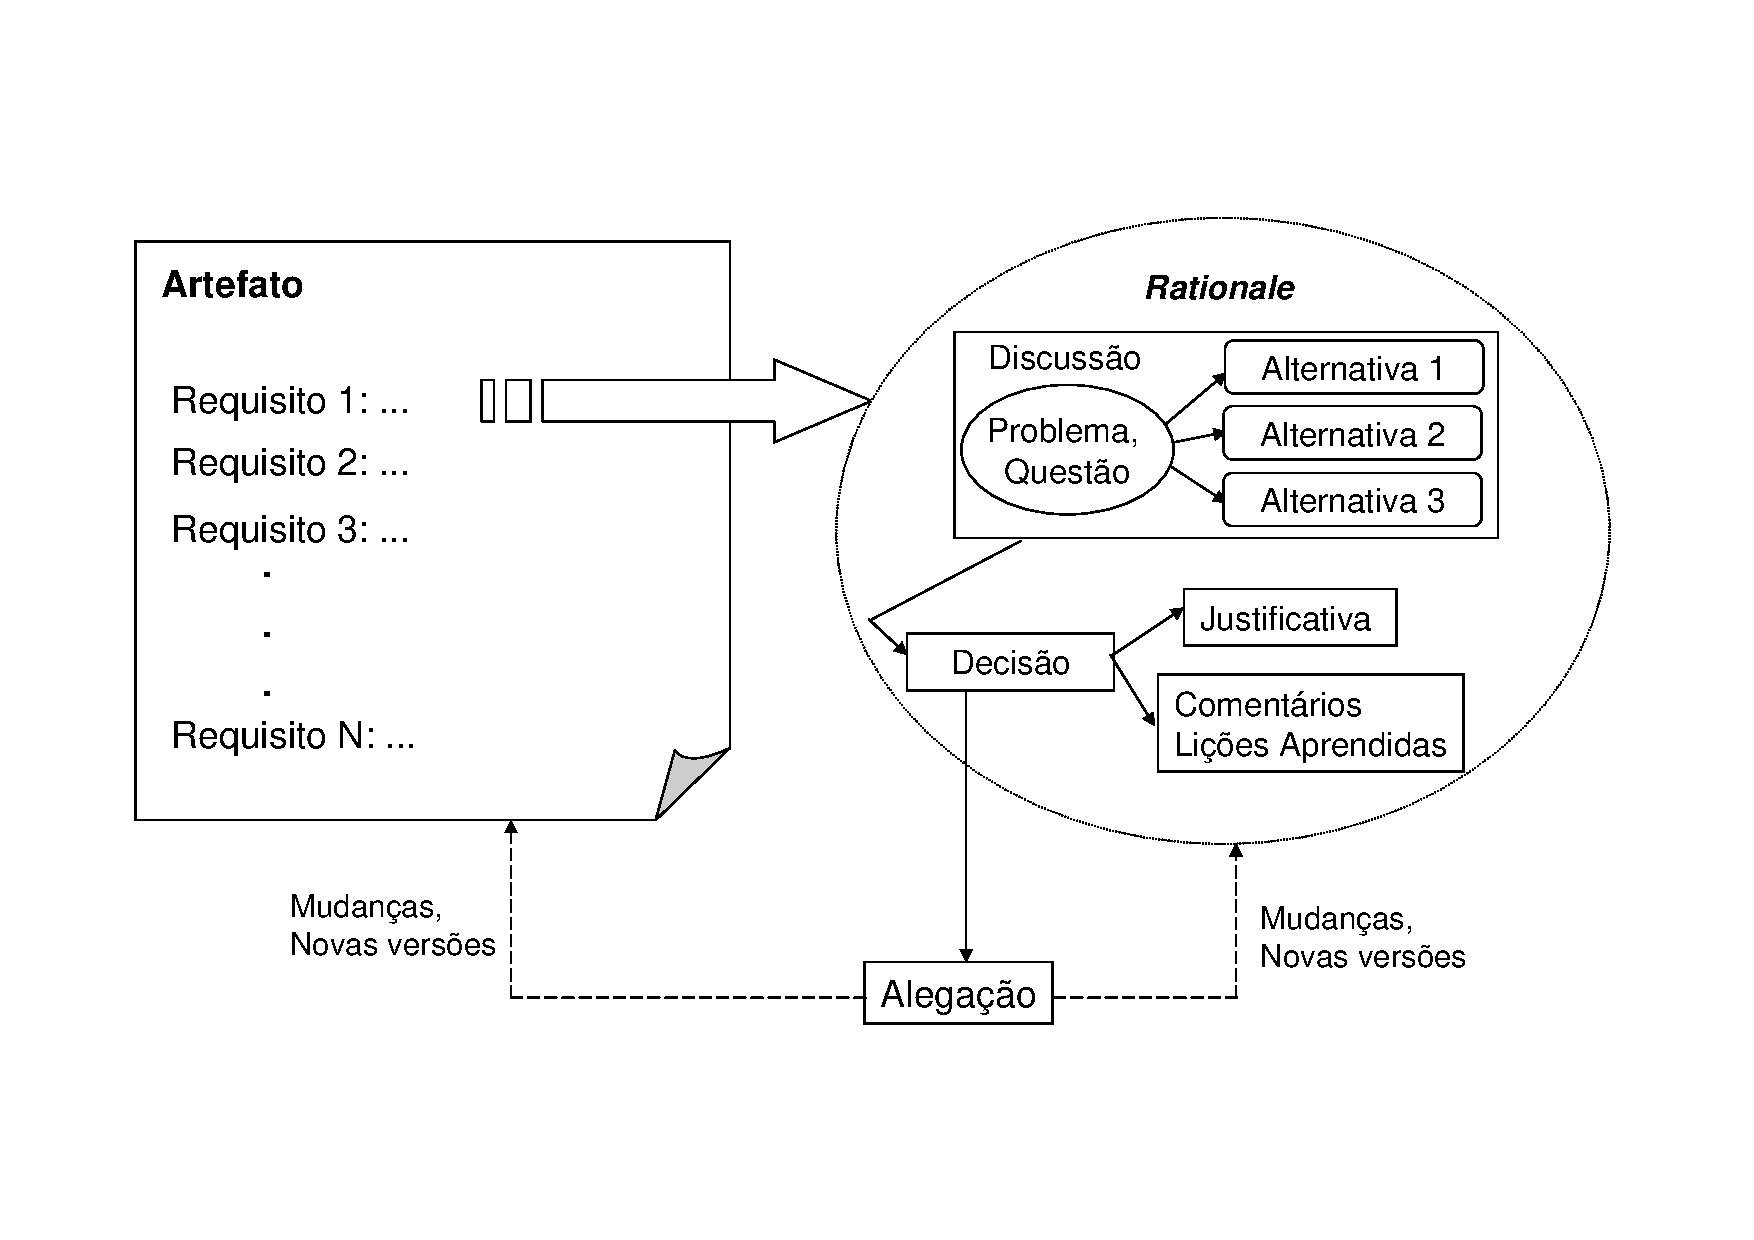
\includegraphics [width=0.85\textwidth]{modelo_dr.pdf}
  \caption {Modelo de representa��o de {\it design rationale} para o contexto de desenvolvimento de projetos de pesquisa em software}
  \label{dr_saci}
\end{figure}


\begin{itemize}

\item {\it Artefato}: representa o artefato de software que cont�m os requisitos elicitados. 

\item {\it Requisito}: representa um requisito funcional ou n�o funcional do sistema. D�vidas ou problemas relacionados � elicita��o dos requisitos levam a discuss�o ou reflex�o. Como resultado, tal discuss�o entre os participantes do desenvolvimento de um projeto pode melhorar o entendimento e o detalhamento dos requisitos. 

\item {\it Problema, Quest�o}: representam os questionamentos ou as d�vidas que surgem na fase de elicita��o dos requisitos do projeto. Est� relacionado a qualquer problema ou dificuldade da equipe que leve a uma discuss�o.   

\item {\it Alternativas}: representam poss�veis solu��es para as quest�es ou d�vidas

\item {\it Decis�o}: representa a indica��o da alternativa selecionada. Pode estar relacionada a uma combina��o de alternativas. 

\item {\it Justificativa}: representa uma explica��o sobre ``porque'' determinada decis�o foi tomada. 

\item {\it Coment�rios, Li��es aprendidas}: representam os registros sobre os resultados obtidos a partir das decis�es que foram tomadas, sobre trabalhos futuros (por exemplo, propor uma modifica��o em determinado requisito para realizar novas investiga��es) e para detalhar as li��es aprendidas.    

\item {\it Alega��o}: representam informa��es que indicam a necessidade de reflex�o em rela��o a requisitos especificados anteriormente ou decis�es tomadas, tendo em vista a realiza��o de novas experi�ncias e a evolu��o do projeto de pesquisa. Por exemplo, problemas ou desvantagens de uma decis�o que foi tomada ou sugest�o para selecionar outra alternativa para o mesmo problema podem ser indicadas.     

\end{itemize}

O relacionamento entre os elementos conceituais do modelo \textbf{DR-SACI} foi definido  de forma que  as setas em \textbf{tra�o cont�nuo} indicam relacionamento de associa��o, mostrando uma rela��o entre dois conceitos, no sentido de complementar a informa��o que se tem sobre eles em um determinado instante. Por exemplo, um problema com suas respectivas alternativas e uma decis�o associada a uma certa justificativa. 

No modelo \textbf{DR-SACI}, as setas em \textbf{tra�o pontilhado} simbolizam o relacionamento de evolu��o de um projeto de pesquisa, ou seja, termos novas vers�es, tanto de um artefato que cont�m os requisitos, quanto da documenta��o de {\it design rationale}, geradas como resultado de uma alega��o a uma decis�o. 


\section{Ferramenta para apoiar o registro de {\it design rationale} de projetos de pesquisa em software}

A partir da proposta do modelo \textbf{DR-SACI} para representa��o de {\it design rationale}, foi realizada uma adapta��o na ferramenta MVCASE\footnote{http://mvcase.dev.java.net} de forma a implementar parcialmente os requisitos e o modelo apresentados na Se��o \ref{mod_re} \citep{pailufor06}.  

A ferramenta MVCASE est� sendo desenvolvida por alunos de gradua��o e p�s-gradua��o da Universidade Federal de S�o Carlos (UFSCar) e do Instituto de Ci�ncias Matem�ticas e de Computa��o (ICMC-USP). Totalmente desenvolvida em Java, � uma ferramenta livre que teve suas origens como uma ferramenta de modelagem \citep{pra00}, e est� evoluindo desde ent�o, com funcionalidades sendo acrescentadas � sua arquitetura, como desenvolvimento baseado em componentes \citep{pra01,almeida02}, integra��o com ambientes de Engenharia de Software \citep{lucredio04jot}, desenvolvimento de software orientado a aspectos \citep{garcia04} e suporte � reutiliza��o de software \citep{lucredio05dissert}. 

A ferramenta MVCASE � extens�vel por meio de {\it plug-ins}. Assim, os desenvolvedores podem adicionar funcionalidades extras �s fun��es b�sicas de modelagem, sem a necessidade de modificar seu c�digo-base. Um desenvolvedor pode incluir funcionalidades em \textit{plug-ins} que podem ser instalados facilmente na ferramenta. Um dos \textit{plug-ins} desenvolvidos para a MVCASE trata a representa��o de {\it design rationale}. 

Na Figura \ref{mvcase} � apresentada uma tela da ferramenta MVCASE indicando a implementa��o do modelo de representa��o de {\it design rationale}. Pode ser observado na figura que um elemento correspondente a um item de {\it design rationale} foi disponibilizado na paleta de elementos gr�ficos (indicado por (1)). Utilizando o bot�o, � poss�vel incluir, em qualquer diagrama suportado pela ferramenta, textos referentes � documenta��o segundo o modelo apresentado na Figura \ref{dr_saci}. O texto inclu�do fica ent�o vis�vel em uma caixa (indicado por (2)), dividida em quatro compartimentos: {\it Problema, quest�o e alternativa} (representados por ``P''); {\it Decis�es} (representadas por ``D''); {\it Justificativas} (representados por ``J'') e {\it Coment�rios e Li��es Aprendidas} (representado por ``Comments''). � poss�vel associar um item de {\it design rationale} diretamente a um determinado elemento do diagrama, por meio de uma linha pontilhada.

\begin{figure} [!ht]
 \centering
  \bfseries
  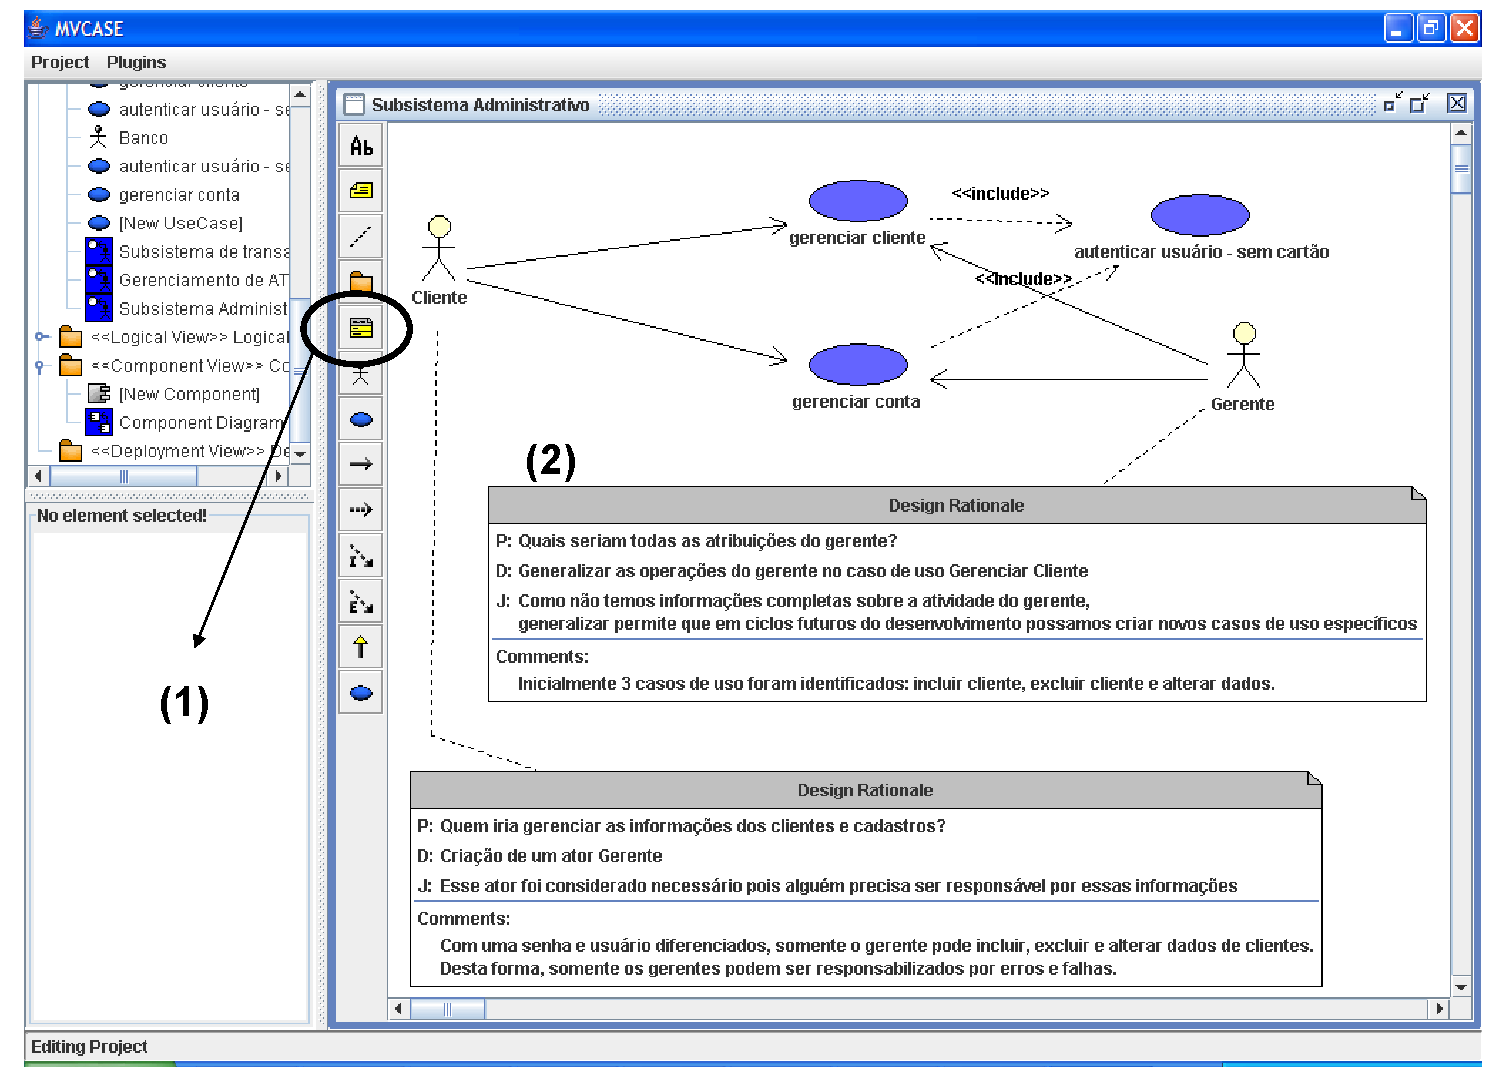
\includegraphics [width=0.95\textwidth]{fig_mvc.pdf}
  \caption{Exemplo de uso da ferramenta MVCASE em que informa��es de {\it design rationale} foram capturadas}
  \label{mvcase}
\end{figure}

Conforme observado por \cite{RegHuAtwSun00}, diversos fatores contribuem para que informa��es de {\it design rationale} n�o sejam capturadas na pr�tica durante o desenvolvimento de projetos. Com a realiza��o deste trabalho (elabora��o do modelo proposto e implementa��o na MVCASE), buscou-se diminuir os efeitos desses fatores e motivar os desenvolvedores para a captura das informa��es. Um dos fatores est� relacionado ao fato de geralmente se propor a utiliza��o de uma nova ferramenta para captura de {\it design rationale}, o que gera uma sobrecarga adicional ao processo de software. Na ferramenta MVCASE, � poss�vel incluir as informa��es nos pr�prios diagramas, sem a necessidade de utilizar outra ferramenta. Outro fator apresentado pelos autores � que os sistemas de {\it design rationale} n�o suprem as necessidades espec�ficas de determinados contextos, por exemplo, uma empresa ou um determinado ambiente. No caso da ferramenta MVCASE, foi implementado um modelo diferenciado, em que foi considerado o dom�nio de desenvolvimento de pesquisas em software.


\section{Experimento envolvendo o modelo de {\it design rationale} e a ferramenta MVCASE} \label{exp_dr}

Foi realizado um experimento em duas disciplinas do curso de Ci�ncia da Computa��o do ICMC-USP. Os modelos IBIS	e DR-SACI foram utilizados, constituindo o tratamento 1 e o tratamento 2, respectivamente. Foi solicitado aos estudantes que capturassem e registrassem {\it design rationale} para os projetos que foram propostos, que deveriam ser desenvolvidos em grupo e de forma colaborativa.   

O experimento consistiu da an�lise de tr�s diferentes projetos de software, com um n�vel similar de dificuldade, considerando-se o n�mero de requisitos e o n�mero de classes do software. 

O enunciado do primeiro projeto estava relacionado � distribui��o de disciplinas para professores de uma universidade (sistema 1, desenvolvido por estudantes da disciplina 1, usando o modelo IBIS); o do segundo projeto estava relacionado ao controle de bilhetes eletr�nico para transporte municipal (sistema 2, desenvolvido por estudantes da disciplina 2, usando o modelo DR-SACI);  e o do terceiro projeto estava relacionado ao controle de caixa eletr�nico de um banco (sistema 3, desenvolvido por estudantes da disciplina 2, usando o modelo DR-SACI). As disciplinas 1 e 2 foram respectivamente: ``Sistemas de Informa��o'' e ``An�lise e Projeto Orientados a Objetos''.


Nas sub-se��es seguintes s�o apresentadas as atividades cumpridas para a defini��o, o planejamento e a execu��o de experimentos, de acordo com os {\it guidelines} recomendados por \cite{Woh2000}, envolvendo o modelo DR-SACI e a ferramenta MVCASE \citep{pai07}. 

\subsection{Defini��o do experimento}

\noindent{\bf Objeto de estudo}: modelo para registro de {\it design rationale} para o contexto de desenvolvimento de projetos de pesquisa em software (DR-SACI).  \\

\noindent{\bf Proposta}: avaliar o modelo DR-SACI em rela��o � motiva��o para registro de {\it design rationale} e sua utilidade na manuten��o e evolu��o de software desenvolvidos em projetos de pesquisa.\\

\noindent{\bf Foco qualitativo}: efic�cia do modelo DR-SACI.\\

\noindent{\bf Perspectiva}: o experimento foi realizado sob o ponto de vista de estudantes do curso de gradua��o do ICMC-USP.\\

\noindent{\bf Contexto}: foram apresentadas diferentes especifica��es de requisitos aos estudantes e foi solicitado que cumprissem atividades de desenvolvimento e manuten��o de software. Foi oferecido treinamento (aproximadamente 3 horas) sobre conceitos de {\it design rationale} e sobre os modelos e as ferramentas utilizadas. Estudantes da disciplina 1 cursavam o oitavo per�odo do curso e os estudantes da disciplina 2 cursavam o s�timo per�odo. O estudo envolvendo o modelo IBIS foi realizado no primeiro semestre de 2005 e o estudo envolvendo o modelo DR-SACI foi realizado no primeiro semestre de 2006.   

\subsection{Planejamento do experimento} \label{plano_experi}

\noindent{\bf Sele��o do contexto} o experimento foi realizado por sessenta estudantes divididos em vinte grupos (tr�s estudantes em cada grupo). O experimento foi realizado fora da sala de aula e sem supervis�o e, portanto, os estudantes tiveram a liberdade de determinar seus pr�prios cronogramas para cumprir as atividades propostas. \\

\noindent{\bf Hip�teses}: as hip�teses foram formuladas considerando a Fase 1, em que havia a possibilidade de fazer an�lise quantitativa.

\begin{description}

\item[{\bf Hip�tese nula (H0)}]: a quantidade de itens de {\it design rationale} registrados usando o modelo DR-SACI � menor ou o mesmo que a quantidade de itens de {\it design rationale} registrados usando um modelo tradicional.  

\item[{\bf Hip�tese alternativa (H1)}]: a quantidade de itens de {\it design rationale} registrados usando o modelo DR-SACI � maior que a quantidade de itens de {\it design rationale} registrados usando um modelo tradicional.

\end{description}

\noindent{\bf Projeto do experimento}: o experimento foi projetado para ser executado em duas fases. Na Fase 1, o foco estava na modelagem dos tr�s sistemas, usando a linguagem UML. Os estudantes das duas disciplinas cumpriram esta fase. Na Fase 2, foi solicitado aos estudantes que tentassem compreender os projetos desenvolvidos por outros grupos para que pudessem realizar uma atividade de manuten��o que foi proposta. Apenas os estudantes da disciplina 2 participaram desta segunda fase. Os grupos que desenvolveram o sistema 2 realizaram a manuten��o no sistema 3 e vice-versa. 

Na Fase 1, o objetivo foi fazer uma an�lise quantitativa dos resultados, ou seja, para cada um dos sistemas foi contado o n�mero de itens de {\it design rationale} registrados pelos estudantes na fase de an�lise de requisitos. No modelo DR-SACI foi considerado como um item de {\it design rationale}, um conjunto de informa��es contendo problema - alternativa(s) - decis�o - justificativa (coment�rios s�o opcionais). Para o modelo IBIS, cada conjunto de informa��es de quest�o - posi��es - argumentos foi contado como um item de {\it design rationale}. %O objetivo foi avaliar se houve melhoria em rela��o � motiva��o dos estudantes para a captura de {\it design rationale} quando o modelo DR-SACI foi usado, resultando em uma quantidade maior de itens de {\it design rationale} em compara��o com o uso do modelo IBIS. %Um ponto negativo � que n�o foi avaliada a import�ncia das informa��es registradas em atividades de manuten��o usando ambos os modelos.   

Na Fase 2, o objetivo foi fazer uma an�lise qualitativa dos resultados, ou seja, avaliar a import�ncia de {\it design rationale} na evolu��o e manuten��o do software. Aproximadamente metade dos grupos p�de acessar e avaliar a import�ncia das informa��es de {\it design rationale} produzidas na Fase 1. Os grupos que n�o utilizaram as informa��es de {\it design rationale} produzidas na Fase 1 puderam avaliar o quanto as informa��es poderiam facilitar o entendimento dos projetos durante a realiza��o da manuten��o.    

Na Tabela \ref{exp1} s�o apresentadas informa��es relacionadas �s duas fases do experimento, em rela��o aos grupos que estiveram respons�veis por cumpri-las e aos sistemas que foram utilizados (\small Legenda: \sffamily DDP = sistema para Distribui��o de Disciplinas para Professores; CBE = sistema para Controle de Bilhetes Eletr�nicos para transporte municipal; CCE = sistema para Controle de Caixa Eletr�nico de um banco).   \\

\begin{table}[!h]
\begin{center}
\caption{Projeto do experimento}\label{exp1}
%\begin{tabular}{|c|c|c|c|}
\begin{tabular}{|p{1.7cm}|p{2.2cm}|p{3.5cm}|p{3.3cm}|p{2.4cm}|}
\hline
{\bf \footnotesize Disciplina} & {\bf \footnotesize Identificador do grupo} & {\bf \footnotesize \centering Fase 1:\\ \centering An�lise requisitos} & {\bf \footnotesize \centering Fase 2:\\  \centering Manuten��o} & \bf \footnotesize Uso de {\it design rationale} \\\hline
\hline  \centering 1 &  \centering 1 &  \small \sffamily  \centering DDP & -- & --\\
\hline  \centering 1 &  \centering 2 &  \small \sffamily  \centering DDP & -- & --\\
\hline  \centering 1 &  \centering 3 &  \small \sffamily  \centering DDP & -- & --\\
\hline  \centering 1 &  \centering 4 &  \small \sffamily  \centering DDP & -- & --\\
\hline  \centering 1 &  \centering 5 &  \small \sffamily  \centering DDP & -- & --\\
\hline  \centering 1 &  \centering 6 &  \small \sffamily  \centering DDP & -- & --\\
\hline  \centering 1 &  \centering 7 &  \small \sffamily  \centering DDP & -- & --\\
\hline  \centering 1 &  \centering 8 &  \small \sffamily  \centering DDP & -- & --\\
\hline  \centering 1 &  \centering 9 &  \small  \sffamily  \centering DDP & -- & -- \\
\hline  \centering 2 &  \centering 10 & \small  \sffamily  \centering CBE &  \sffamily  \centering CCE  & \small  \textit{sim} \\
\hline  \centering 2 &  \centering 11 & \small  \sffamily  \centering CCE &  \sffamily  \centering CBE  & \small   \textit{sim} \\
\hline  \centering 2 &  \centering 12 & \small  \sffamily  \centering CBE &  \sffamily  \centering CCE  & \small  n�o \\
\hline  \centering 2 &  \centering 13 & \small  \sffamily  \centering CCE &  \sffamily  \centering CBE  & \small   n�o \\
\hline  \centering 2 &  \centering 14 & \small  \sffamily  \centering CBE &  \sffamily  \centering CCE  & \small  \textit{sim} \\
\hline  \centering 2 &  \centering 15 & \small  \sffamily  \centering CCE &  \sffamily  \centering CBE  & \small  \textit{sim} \\
\hline  \centering 2 &  \centering 16 & \small  \sffamily  \centering CBE &  \sffamily  \centering CCE  & \small   n�o \\
\hline  \centering 2 &  \centering 17 & \small  \sffamily  \centering CCE &  \sffamily  \centering CBE  & \small  n�o \\
\hline  \centering 2 &  \centering 18 & \small  \sffamily  \centering CBE &  \sffamily  \centering CCE  & \small   \textit{sim} \\
\hline  \centering 2 &  \centering 19 & \small  \sffamily  \centering CCE &  \sffamily  \centering CBE  & \small  \textit{sim} \\
\hline  \centering 2 &  \centering 20 & \small  \sffamily  \centering CBE &  \sffamily  \centering CCE  & \small   n�o \\
\hline
\end{tabular}
\end{center}
\end{table}

\normalsize
\normalfont
\subsubsection {Vari�veis independentes} 

\noindent {\it Metodologia usada} -- na Fase 1 (modelagem do software), aproximadamente metade dos estudantes usou o modelo IBIS e os demais usaram o modelo DR-SACI. Na Fase 2 (manuten��o do software), apenas o modelo DR-SACI foi usado, realizando-se a troca de projetos entre os grupos. Os itens de {\it design rationale} elaborados na Fase 1 foram disponibilizados a aproximadamente metade dos estudantes durante a Fase 2. \\

\noindent {\it Experi�ncia dos estudantes e �rea de interesse}: os estudantes possu�am experi�ncia pr�via em an�lise orientada a objetos e interesse em diferentes �reas da Ci�ncia da Computa��o.  

\subsubsection {Vari�veis dependentes}

\noindent  {\it Quantidade de itens de {\it design rationale} registrados pelos participantes} -- Conforme mencionado anteriormente, foi definido previamente como os itens seriam contados. Em rela��o � Fase 2, as informa��es subjetivas dos participantes considerando a utilidade de {\it design rationale} na manuten��o de software foi considerada uma vari�vel dependente. \\

\subsubsection {Sele��o dos participantes}

\noindent Os participantes foram escolhidos considerando-se a conveni�ncia. A divis�o dos estudantes em grupos n�o foi aleat�ria, pois eles puderam fazer as escolhas dos membros de acordo com suas vontades. A distribui��o dos sistemas entre os grupos foi aleat�ria na Fase 1 e foi invertida na Fase 2. Os estudantes n�o tiveram a liberdade de escolher entre participar ou n�o do estudo, pois o experimento constituiu parte de um projeto obrigat�rio que deveria ser desenvolvido nas disciplinas. Portanto, n�o � poss�vel garantir que os resultados seriam os mesmos se os participantes fossem volunt�rios. 


\subsubsection{Amea�as � validade}

\noindent {\it Validade de conclus�o}: para todos os grupos, os itens de {\it design rationale} foram contados considerando o crit�rio mencionado no item {\it Projeto do experimento}. � importante observar, no entanto, que os estudantes receberam pontos de cr�dito nas disciplinas por suas participa��es no estudo. H� o risco de que o incentivo tenha influenciado os resultados apresentados. Al�m disso, o experimento foi realizado em duas disciplinas diferentes. Se os gurpos s�o muito heterog�neos, � poss�vel que as varia��es que ocorreram devido �s influ�ncias individuais tenham interferido no resultado geral do experimento.       \\

\subsubsection {Validade interna}

\noindent Os tratamentos n�o foram aplicados a todos os participantes, ou seja, � poss�vel que um resultado diferente tivesse sido obtido se os tratamentos fossem trocados entre os grupos. Em rela��o a amea�a � matura��o, a maioria dos participantes aparentemente estava concentrada em suas atividades (n�o houve controle em rela��o a esse efeito). Na Fase 2, em rela��o � instrumenta��o, � importante notar que os resultados s�o dependentes do conte�do dos itens de {\it design rationale} gerados na Fase 1. Portanto, os resultados sobre a utilidade de {\it design rationale} para manuten��o de software s�o influenciados pelas condi��es da base fornecida, por exemplo, completude. Se as informa��es n�o foram registradas adequadamente, os resultados foram afetados negativamente.     

\subsubsection{Validade de constru��o}

\noindent O treinamento em {\it design rationale} n�o foi extensivo e, portanto, os conceitos e as defini��es provavelmente n�o foram claras para alguns estudantes. Poucos tipos de medi��es foram executadas e as conclus�es podem ter sido afetadas negativamente. O fato de que os estudantes estavam desenvolvendo um projeto que � parte de uma disciplina pode ser considerado uma amea�a, pois eles poderiam tentar manipular as informa��es para melhorar suas notas. No entanto, esse fato n�o foi considerado, pois os estudantes foram informados a respeito da import�ncia da acur�cia das informa��es. Al�m disso, o professor da disciplina 1 n�o foi o mesmo da disciplina 2, o que pode ter causado diferen�as no direcionamento da proposta das atividades.

\subsubsection{Validade externa}

\noindent N�o � poss�vel generalizar os resultados para diferentes contextos pois, para a elabora��o do modelo considerado no experimento (DR-SACI) foram enfatizadas caracter�sticas comuns do contexto de desenvolvimento de projetos de pesquisa. Considerou-se aceit�vel a realiza��o dos experimentos com estudantes sobre um modelo voltado para o desenvolvimento de projetos de pesquisa, pois sabe-se que em geral os estudantes s�o membros das equipes que desenvolvem os projetos.  

\subsubsection{Instrumenta��o}

\noindent O material fornecido aos participantes para a execu��o dos experimento foi composto por: {\it guidelines} para executar o experimento, documento de requisitos do sistema (apenas o necess�rio para cada grupo), documentos contendo descri��es do modelo IBIS e do modelo DR-SACI (apenas o necess�rio para cada grupo), documentos descrevendo diagrama de casos de uso e diagrama de classes, planilhas para coletar os dados do experimento.  


\subsection{Realiza��o do experimento}

\subsubsection{Prepara��o}

\noindent Como parte do treinamento, foram ministradas aulas sobre {\it design rationale} (conceitos, modelos, etc) e an�lise orientada a objetos. Os artefatos indicados no item {\it Instrumenta��o} foram disponibilizados na {\it web}. \\

\subsubsection{Participantes}

\noindent Os estudantes possu�am conhecimento pr�vio em Engenharia de Software, mas eles n�o possu�am conhcimento sobre conceitos de {\it design rationale}.  \\

\subsubsection{Realiza��o do experimento}

\noindent Inicialmente, a descri��o do sistema com o qual o trabalho seria realizado foi apresentado aos estudantes, bem como as tarefas que deveriam ser cumpridas (modelagem do sistema e registro de {\it design rationale}). Foi considerado que, avaliar a motiva��o dos estudantes em termos da quantidade de itens de {\it design rationale} capturados n�o era suficiente, ou seja, seria fundamental obter alguma informa��o sobre a qualidade das informa��es em rela��o � utilidade na fase de manuten��o dos projetos. Dessa forma, foi proposta uma atividade de manuten��o para estudantes da disciplina 2, usando o modelo DR-SACI. Os estudantes da disciplina 1 n�o participaram porque o tema de manuten��o de software n�o fazia parte do programa do curso. Os projetos desenvolvidos por estudantes da disciplina 2 foram trocados entre os grupos e um novo requisito foi adicionado. Foi solicitado que as modifica��es necess�rias fossem realizadas. Os dados resultantes das duas fases foram coletados da seguinte forma: ap�s a Fase 1, a documenta��o disponibilizada pelos estudantes das duas disciplinas foi examinada e o n�mero de itens de {\it design rationale} foi contado. Durante a execu��o da Fase 2, os grupos registraram em um question�rio as suas opini�es sobre a import�ncia das informa��es de {\it design rationale} durante a manunte��o de software. As respostas obtidas tamb�m foram contabilizadas.    \\

\subsubsection{Valida��o dos dados}

\noindent O question�rio distribu�do aos participantes foram checados com o objetivo de garantir que foram preenchidos corretamente. Os registros obtidos foram satisfat�rios e nenhum question�rio foi descartado. 

\subsection{Resultados dos experimentos}

Primeiramente, as hip�teses ser�o analisadas, considerando-se os dados quantitativos. Em seguida, as respostas obtidas para o question�rio ser�o discutidas. 

Os resultados da an�lise estat�stica descritiva considerando-se as duas disciplinas s�o apresentados na Tabela \ref{quantid}. A terceira coluna apresenta os valores m�dios relacionados � quantidade de itens de {\it design rationale} registrados pelos estudantes usando ambos os modelos. A diferen�a entre os valores fornece uma evid�ncia (embora n�o prove) de que a motiva��o para registro de {\it design rationale} melhorou quando o modelo DR-SACI foi utilizado. 

\begin{table}[h]
\begin{center}
\caption{Resultados quantitativos em rela��o � captura de {\it design rationale}}\label{quantid}
\begin{tabular}{|c|c|c|c|}
%\begin{tabular}{|l|c|c|c|}
%\begin{tabularx}{|X|X|X|}
\hline
 & {\bf \footnotesize Quantidade de grupos} & \bf \footnotesize �tens de {\it design rationale} &  {\bf \footnotesize Desvio padr�o} \\
 &      & \footnotesize (valor m�dio) & \\\hline
\hline \footnotesize Modelo IBIS       &      &      &      \\
       \footnotesize (disciplina 1)    &   9  & 3,78 & 3,49 \\
\hline \footnotesize Modelo DR-SACI    &      &      &      \\
       \footnotesize (disciplina 2)    &  11  & 8,36 & 2,42  \\
\hline
\end{tabular}
\end{center}
\end{table}

Um gr�fico {\it box plot} foi gerado para facilitar a visualiza��o dos dados (Figura \ref{box}). A partir da figura � poss�vel observar que h� um padr�o que indica que a quantidade de itens de {\it design rationale} registrada foi maior quando o modelo DR-SACI foi utilizado.   

\begin{figure} [!ht]
 \centering
  \bfseries
  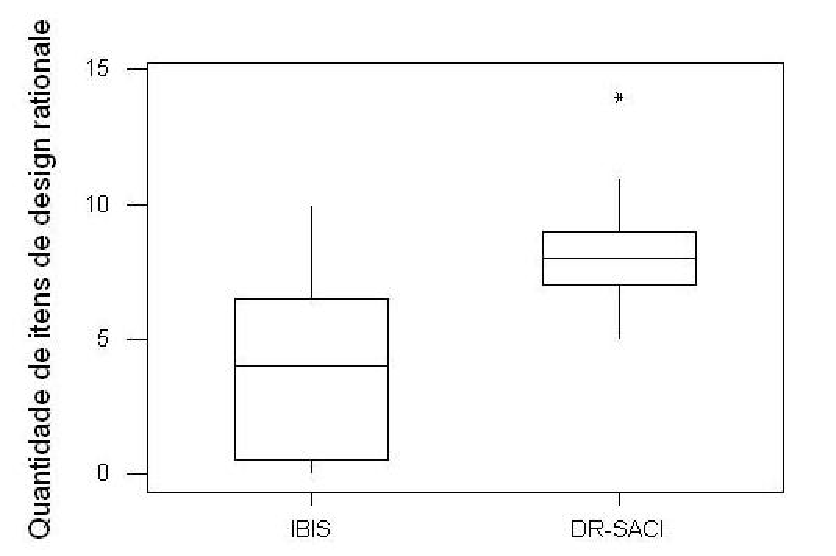
\includegraphics [width=0.85\textwidth]{box.pdf}
  \caption{Quantidade de itens de {\it design rationale} registrados em rela��o ao uso dos modelos IBIS e DR-SACI}
  \label{box}
\end{figure}

Os dados coletados foram testados em rela��o � normalidade por meio do teste Anderson-Darling, utilizando-se a ferramenta MINITAB. Os testes de hip�tese para normalidade dos dados provenientes do uso do modelo IBIS (p-value=0,470) e dos dados provenientes do uso do modelo DR-SACI (p-value=0,069) n�o foram rejeitados, considerando o n�vel de signific�ncia de 5\%. Os gr�ficos gerados s�o apresentados nas Figuras \ref{norma_ibis} e \ref{norma_saci}.   

\begin{figure} [!ht]
 \centering
  \bfseries
  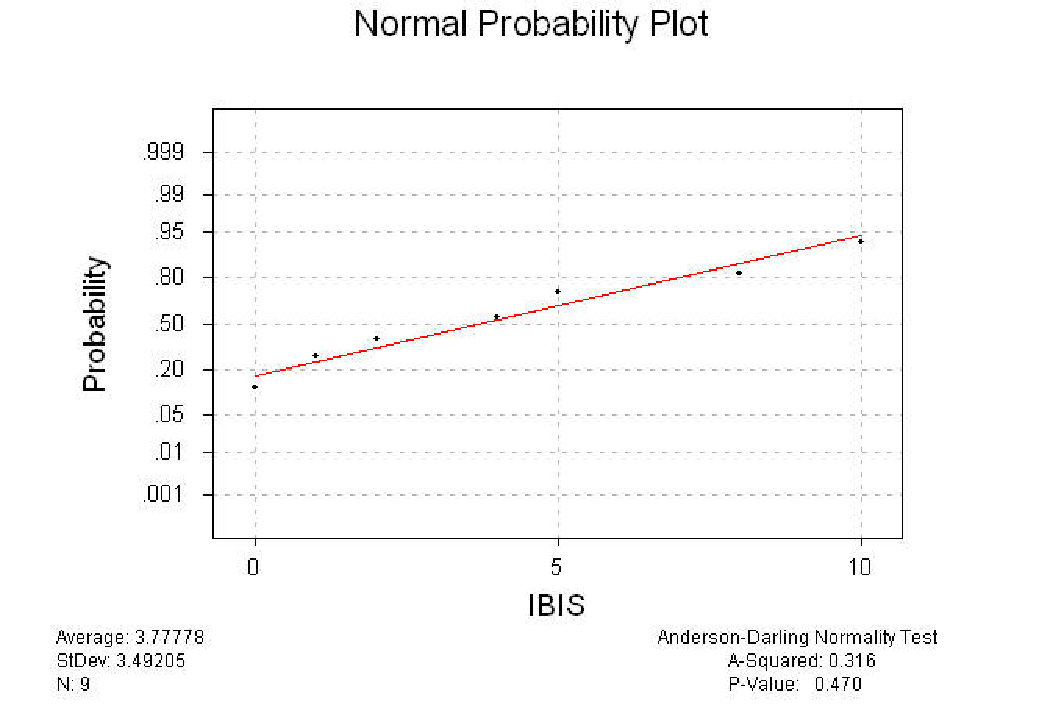
\includegraphics [width=0.85\textwidth]{normalidade_ibis.pdf}
  \caption{Resultados do teste de normalidade dos dados obtidos com o uso do modelo IBIS}
  \label{norma_ibis}
\end{figure}

\begin{figure} [!ht]
 \centering
  \bfseries
  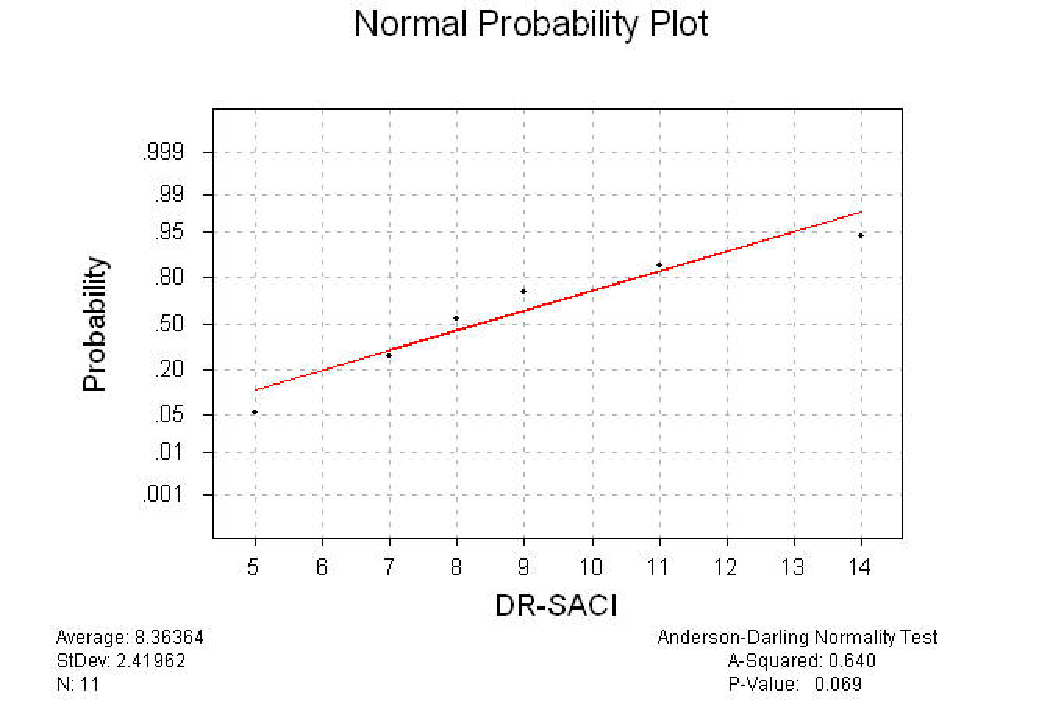
\includegraphics [width=0.85\textwidth]{normalidade_saci.pdf}
  \caption{Resultados do teste de normalidade dos dados obtidos com o uso do modelo DR-SACI}
  \label{norma_saci}
\end{figure}

Foi realizado um t-test bilateral com as duas amostras presumindo vari�ncias equivalentes. O resultado indicou que o n�mero de itens de {\it design rationale} registrado para grupos que usaram o modelo DR-SACI foi significativamente maior em compara��o ao uso do modelo IBIS (p-value=0,0027). Com este resultado, portanto, � poss�vel rejeitar a hip�tese nula (H0) e concluir que h� uma diferen�a significativa entre os resultados obtidos quando o modelo IBIS e DR-SACI foram utilizados.    

Foi solicitado, ainda, que os estudantes da disciplina 2 registrassem suas opini�es durante o experimento sobre alguns t�picos espec�ficos. Foi perguntado aos grupos que usaram {\it design rationale} durante a fase de manuten��o se as informa��es apresentadas (em rela��o �s categorias do modelo DR-SACI) foram suficientes para auxiliar a compreens�o do projeto. Como apresentado na Figura \ref{sub1}, a maioria dos estudantes indicou que as categorias do modelo foram satisfat�rias. 

\begin{figure} [!ht]
 \centering
  \bfseries
  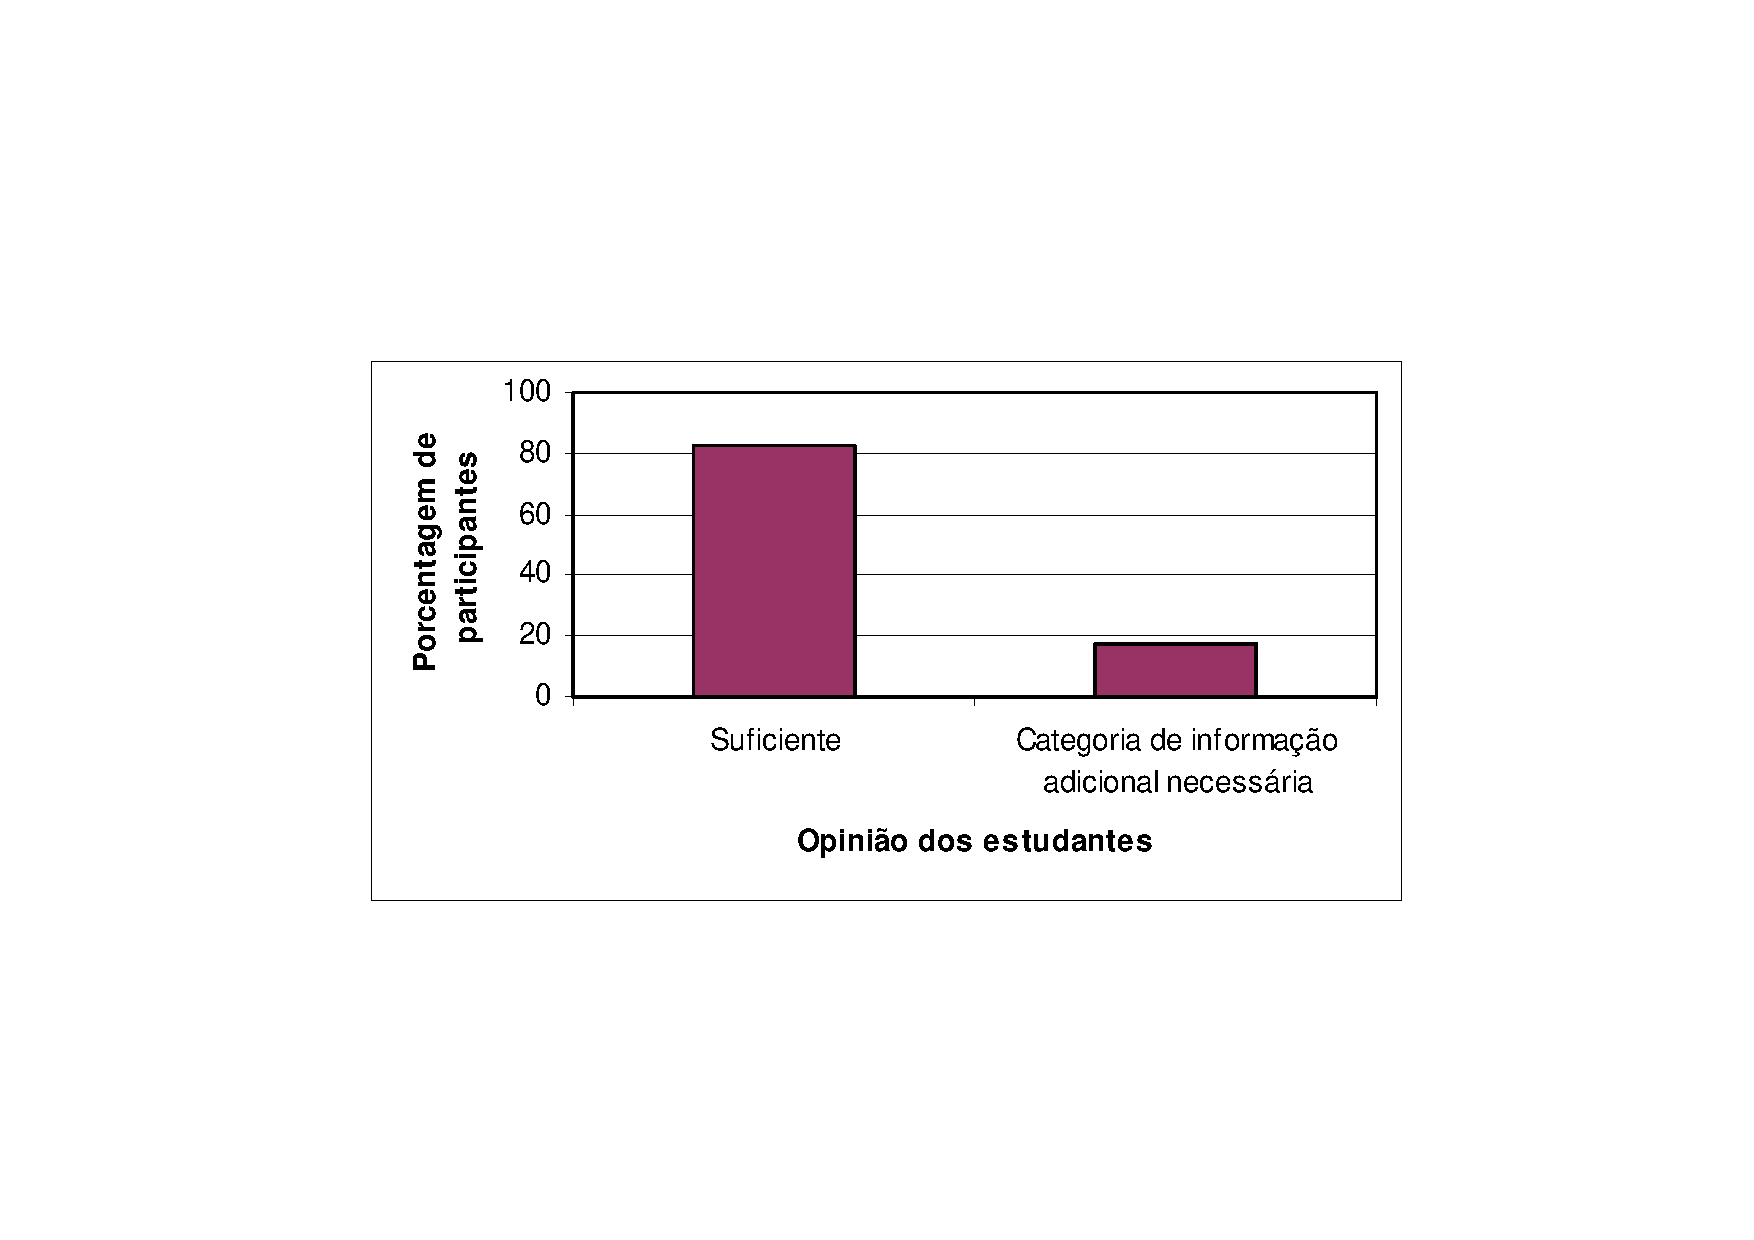
\includegraphics [width=0.70\textwidth]{fig5.pdf}
  \caption{Resultados da avalia��o da estrutura do modelo DR-SACI}
  \label{sub1}
\end{figure}

Os grupos que usaram {\it design rationale} durante a fase de manuten��o tamb�m avaliaram se as informa��es disponibilizadas ajudaram a compreender o projeto desenvolvido por outro grupo. Como apresentado na Figura \ref{sub2}, aproximadamente 80\% dos estudantes indicou que as informa��es de {\it design rationale} foram importantes ou muito importantes. 

\begin{figure} [!ht]
 \centering
  \bfseries
  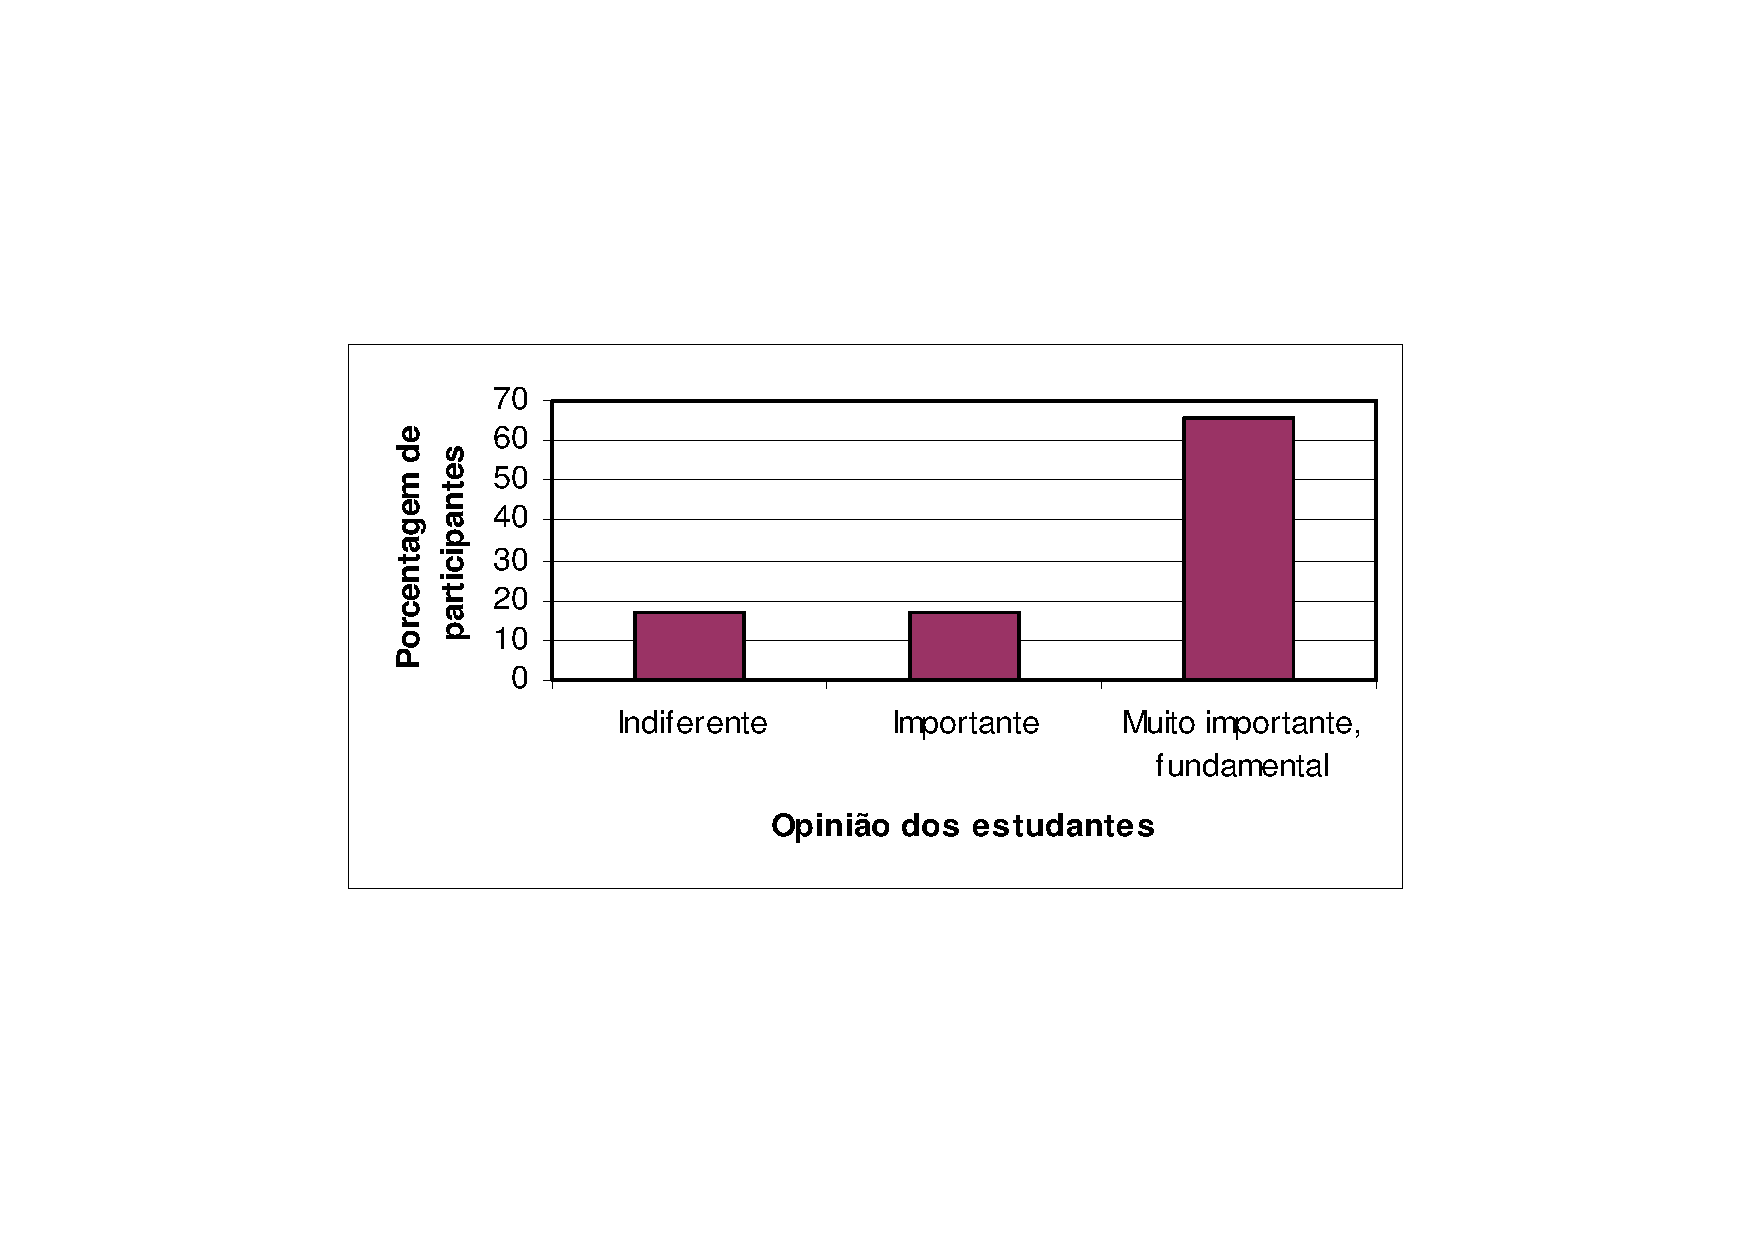
\includegraphics [width=0.70\textwidth]{fig6.pdf}
  \caption {Resultados da avalia��o da import�ncia do modelo DR-SACI na fase de manuten��o}
  \label{sub2}
\end{figure}


Foi perguntado aos grupos que realizaram a manuten��o sem {\it design rationale} se, ao surgirem d�vidas durante a etapa de compreens�o do projeto, era poss�vel encontrar as respostas nos diagramas disponibilizados ou se informa��es adicionais teriam sido relevantes. Conforme apresentado na Figura \ref{sub3}, 60\% dos participantes julgaram importante a disponibiliza��o das informa��es adicionais. Por outro lado, 40\% dos estudantes indicou que as informa��es adicionais n�o poderiam ajud�-los, porque as d�vidas surgiram principalmente em rela��o ao novo requisito considerado. 

\begin{figure} [!ht]
 \centering
  \bfseries
  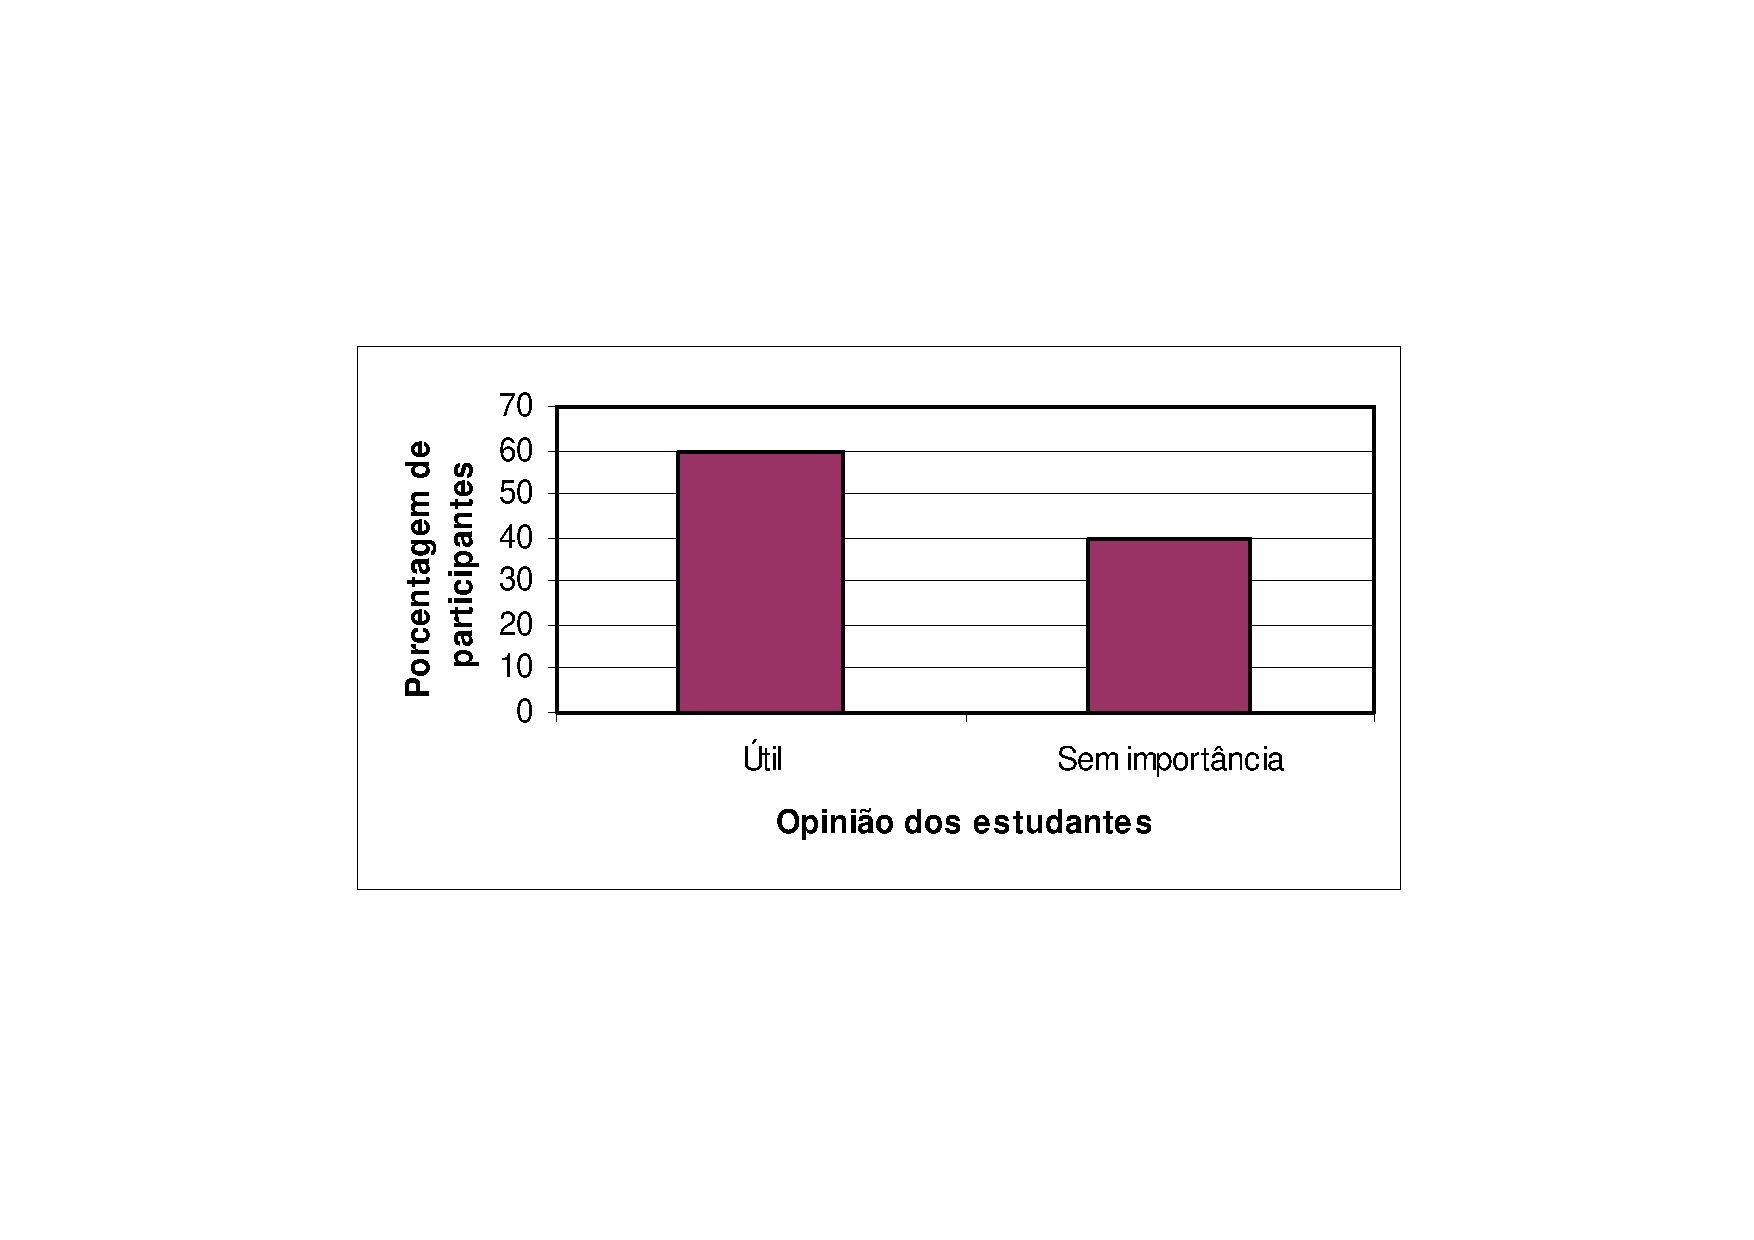
\includegraphics [width=0.70\textwidth]{fig7.pdf}
  \caption {Opini�o dos estudantes que realizaram a manuten��o sem o uso de {\it design rationale}}
  \label{sub3}
\end{figure}


Finalmente, � importante destacar outro resultado positivo relacionado ao experimento. Durante a fase de manuten��o, o registro de {\it design rationale} n�o foi solicitado aos estudantes. No entanto, aproximadamente 65\% deles fez o registro de tais informa��es. Este resultado foi observado como uma forte evid�ncia de que, uma vez que os estudantes tenham compreendido a import�ncia de {\it design rationale} em documenta��o de software, eles estar�o motivados a usar a abordagem em projetos futuros.    

\section{Compara��o entre propostas para registro de {\it design rationale} em projetos de pesquisa}

Conforme apresentado na Se��o \ref{sec_kim}, a �nica proposta encontrada na literatura envolvendo {\it design rationale} no contexto de projetos de pesquisa foi apresentada por \cite{kim93}. Os autores propuseram uma adapta��o do modelo IBIS para o contexto de desenvolvimento de pesquisas cient�ficas colaborativas. No entanto, as atividades cumpridas para elabora��o do modelo e os resultados experimentais de sua avalia��o n�o foram indicados. 

Considerando-se a import�ncia que a Engenharia de Software experimental tem assumido nos �ltimos anos \citep{Woh2000}, diferentemente da metodologia adotada por Kim et al, na proposta do modelo DR-SACI, a experimenta��o est� sendo considerada uma importante atividade para auxiliar a avalia��o e a melhoria da proposta. Um novo estudo de caso foi proposto e realizado no segundo semestre de 2006 no ICMC-USP, por�m seus resultados ainda n�o foram contabilizados. Certamente esses novos dados ser�o importantes para permitir tirar conclus�es sobre a efic�cia do modelo. 

O principal elemento que diferencia a proposta apresentada nesta tese � a ado��o da abordagem de registrar principalmente ``o que o pesquisador fez''. Assim, o registro de alternativas que n�o foram implementadas e de argumentos para os quais n�o h� avalia��o n�o s�o consideradas como foco da proposta. O objetivo principal � indicar as decis�es e as justificativas de forma expl�cita, colaborando para o entendimento dos projetos na fase de manuten��o.   

\section{Considera��es finais}

Neste cap�tulo foi apresentado o modelo de {\it design rationale} elaborado para o desenvolvimento de projetos de pesquisa. Foram descritas as fases cumpridas para obten��o do modelo e os resultados parciais obtidos (por exemplo, a proposta dos requisitos e a adapta��o realizada na ferramenta MVCASE). 

A necessidade de realiza��o de novos estudos de caso torna-se evidente. Em particular, observa-se a import�ncia em realiz�-los no pr�prio ambiente de desenvolvimento de pesquisas. A experi�ncia obtida com a realiza��o do estudo descrito na Se��o \ref{exp_dr} ser� importante na defini��o, no planejamento e na realiza��o de outros experimentos.    


\chapter{Conclus�es} \label{acabou}


\section{Contribui��es}

Este trabalho teve por objetivo identificar um processo para desenvolvimento de projetos de pesquisa envolvendo software, tendo em vista o aux�lio � evolu��o desses projetos. Uma das principais dificuldades relatadas na literatura est� relacionada � car�ncia de documenta��o em um ambiente em que h� alta rotatividade dos membros que participam das equipes. Esta foi uma importante motiva��o para que o processo de documenta��o fosse investigado de forma mais detalhada, considerando-se a abordagem de {\it design rationale}. 

As principais contribui��es deste trabalho e as experi�ncias relacionadas podem ser resumidas conforme apresentadas a seguir:

\begin{enumerate}

\item Identifica��o de um processo para desenvolvimento de projetos de pesquisa, utilizando-se uma abordagem sistem�tica proposta na literatura. O uso da abordagem proposta por Humphrey para a defini��o do processo foi relevante, pois indicou etapas fundamentais, como a identifica��o de requisitos para o processo, que guiaram efetivamente o desenvolvimento da proposta. Al�m disso, acredita-se que a documenta��o gerada com o cumprimento de cada etapa contribuir� para a evolu��o e melhoria da proposta.    

\item Identifica��o de um modelo de {\it design rationale} para projetos de pesquisa, considerando-se caracter�sticas do dom�nio. Estudos de caso foram realizados no decorrer do trabalho e os resultados obtidos, as experi�ncias realizadas e as li��es aprendidas fundamentaram a elabora��o da proposta. Al�m disso, o fato de ter sido cumprido um ciclo de desenvolvimento para a obten��o do modelo, incluindo identifica��o de requisitos, projeto, implementa��o e experimenta��o, foi fundamental no sentido de possibilitar o refinamento gradual da proposta.   

\end{enumerate}    

Nota-se que as contribui��es est�o inseridas em um contexto de pesquisa que est� sendo valorizado atualmente. H� diversos incentivos para que projetos de pesquisa sejam desenvolvidos de forma colaborativa, envolvendo pesquisadores de diferentes �reas de conhecimento, tendo em vista aos avan�os cient�ficos e tecnol�gicos. Como resultado, a comunidade cient�fica est� come�ando a propor discuss�es de amplo alcance em torno do tema de \textbf{processos} para o desenvolvimento de projetos de pesquisa. Um exemplo disso � a realiza��o do {\it First International Workshop on Improving Research Productivity in Computing}\footnote{http://www.iaria.org/conferences2007/IRP.html}, a ser realizado em agosto de 2007 na Fran�a, que tem por objetivo discutir {\it como} os projetos de pesquisa est�o sendo desenvolvidos e quais s�o as alternativas para melhorar os processos utilizados.   

\section{Limita��es} \label{limita}

Algumas limita��es deste trabalho foram:

\begin{itemize}

\item Alguns requisitos identificados pelos usu�rios, por exemplo, gerenciamento de conhecimentos, n�o foram cobertos pois optou-se por propor uma solu��o inicial que dever� ser avaliada, melhorada e estendida de forma incremental; 

\item A descri��o das atividades, tarefas e artefatos do processo � simplificada e oferece apenas uma vis�o geral do trabalho que precisa ser realizado;

\item A abordagem iterativa, mencionada como um requisito de um processo para desenvolvimento de projetos de pesquisa em software, n�o foi experimentada;

\item A avalia��o e a valida��o do processo proposto foram pouco enfatizadas, sendo necess�ria, principalmente, a realiza��o de experimentos reais no contexto de desenvolvimento de projetos de pesquisa colaborativos e distribu�dos;

\item A proposta envolvendo {\it design rationale} n�o foi analisada em rela��o �s atividades de captura e recupera��o das informa��es. � importante averiguar o quanto essas atividades podem ser cumpridas satisfatoriamente quando o modelo � utilizado.  

\end{itemize}

\section{Trabalhos futuros}

Al�m das propostas de trabalhos futuros indicadas nos cap�tulos anteriores, podem ser destacadas:  

\begin{itemize}

\item Definir formalmente a sint�tica e a sem�ntica do processo; 

\item Desenvolver um ambiente que auxilie a execu��o das atividades propostas e o armazenamento e a recupera��o de informa��es relacionadas aos projetos de pesquisa. Uma possibilidade � a investiga��o da adequa��o de ambientes que j� foram desenvolvidos, por exemplo, a esta��o TABA \citep{roch05} nesse escopo. Certamente este ser� um facilitador para o cumprimento das etapas 7 e 8 propostas por Humphrey, que se referem � valida��o e melhoria do processo; 

\item Investigar se os modelos de avalia��o de processos de software atuais s�o aplic�veis ao contexto de desenvolvimento de projetos de pesquisa. Caso n�o sejam, investigar quais elementos devem compor tais modelos. Observa-se que alguns pesquisadores est�o come�ando a se interessar em avaliar os processos que cumprem nos laborat�rios de pesquisa, com o objetivo de atrair e viabilizar novas parcerias com outros centros de pesquisa e com o setor industrial. Um modelo de avalia��o, portanto, complementa a proposta apresentada neste trabalho;

\item Investigar as principais caracter�sticas que definem um ambiente {\it collaboratory} e determinar o quanto a proposta apresentada est� alinhada aos seus objetivos, propondo e realizando as modifica��es necess�rias;

\item Dar continuidade �s investiga��es relacionadas a um modelo de maturidade para o desenvolvimento de projetos de pesquisa envolvendo software, observando a viabilidade em tratar a especializa��o dos n�veis 4 e 5 do CMMI para esse contexto;

\item Realizar experimentos com o modelo de {\it design rationale} em um ambiente de desenvolvimento de pesquisas;

\item Investigar a possibilidade de aplica��o da abordagem de {\it design rationale} como uma forma de capturar o conhecimento dos pesquisadores em rela��o a cada um dos processos apresentados na Figura \ref{fig1};

\item Cobrir os requisitos de {\it evolu��o de design rationale} e {\it informa��es de contexto} do modelo de representa��o, discutidos na Se��o \ref{mod_re}.
  
\end{itemize}


\section{Produ��o cient�fica}

A seguir est�o as refer�ncias das publica��es decorrentes dos estudos realizados e dos resultados obtidos durante o desenvolvimento da pesquisa descrita nesta tese.  

\subsubsection{Artigos completos em peri�dicos}

\begin{enumerate}

\item Paiva, D. M. B.; Freire, A. P.; Lucr�dio, D.; Braga, R. T. V.; Fortes, R. P. M. ``Reinforcing Design Rationale in Software Projects Developed in Academic Environment.'' \textit{International Transactions on Systems Science and Applications}, 2007. Aceito para publica��o.

\item Freire, A. P.; Paiva, D. M. B.; Fortes, R. P. M. ``Implanta��o de Gest�o Descentralizada de Recursos Acad�micos - um estudo de caso.'' \textit{Revista Brasileira de Inform�tica na Educa��o}, v. 12, n. 2, p. 78-85, 2004. 

\end{enumerate}

\subsubsection{Artigos completos em congressos}

\begin{enumerate}

\item Paiva, D. M. B.; Turine, M. A. S.; Fortes, R. P. M. ``Processo de Software Livre em Ambiente Acad�mico: Experi�ncias e Li��es Aprendidas.'' \textit{Proceedings}. In: CLEI 2006 - XXXII Conferencia Latinoamericana de Inform�tica, Chile, 2006.  

\item Paiva, D. M. B.; Lucr�dio, D.; Fortes, R. P. M. ``MVCASE - Incluindo Design Rationale para Aux�lio � Modelagem em Projetos de Pesquisa.'' \textit{Anais.} In: XVIII Sess�o de Ferramentas do XX Simp�sio Brasileiro de Engenharia de Software,  Florian�polis-SC, p. 73-78, 2006.  

\item Paiva, D. M. B.; Fortes, R. P. M. ``Design Rationale in Software Engineering: A Case Study.'' \textit{Proceedings.} In: Seventeenth International Conference on Software Engineering \& Knowledge Engineering (SEKE), Taiwan, p. 342-348, 2005.

\item Paiva, D. M. B.; Manduca, A. M.; Silva, M. A. G.; Quemello, L. J.; Braga, R. T. V.; Fortes, R. P. M.  ``Refor�ando a Comunica��o com Uso de uma Ferramenta de Software Livre em Ensino de Engenharia de Software.'' \textit{Anais.} In: XIII Workshop sobre Educa��o em Computa��o (WEI 2005), XXV Congresso da Sociedade Brasileira de Computa��o (SBC 2005), S�o Leopoldo-RS, 2005. 

\item Paiva, D. M. B.; Fortes, R. P. M. ``Model for Academic Software Development Including Design Rationale Elements.'' \textit{Proceedings.} In: I IFIP Academy on the State of Software Theory and Practice - PhD Colloquium, Porto Alegre-RS, 2005.  

\item Cagnin, M. I.; Paiva, D. M. B.; Maldonado, J. C.; Penteado, R. D.; Fortes, R. P. M.; Germano, R. S. ``From Design Rationale to Reengineering Rationale: Lessons Learned in a Maintenance Pilot Case Study.'' \textit{Proceedings.} In: 4� Jornadas Iberoamericanas de Ingenier�a del Software e Ingenier�a del Conocimiento, Espanha, p. 231-243, 2004.  

\item Paiva, D. M. B.; Freire, A. P.; Sanches, R.; Fortes, R. P. M. ``Definindo, Implantando e Melhorando Processos de Software em Ambiente Acad�mico.'' \textit{Anais.} In: VI Simp�sio Internacional de Melhoria de Processo de Software (SIMPROS), S�o Paulo-SP, p. 71-82, 2004.  

\item Paiva, D. M. B.; Sanches, R.; Fortes, R. P. M. ``Melhoria de Processo de Software no Contexto do Desenvolvimento Acad�mico de uma Agenda na {\it Web}.'' \textit{Anais.}  In: 14o Congresso Internacional de Tecnologia de Software (CITS 2003), Curitiba-PR, p. 56-68, 2003. 

\item Francisco, S. D.; Izeki, C. A.; Paiva, D. M. B.; Fortes, R. P. M. ``Um Sistema de Apoio � Utiliza��o de Design Rationale de Artefatos de Software.'' \textit{Proceedings.} In: CLEI 2003 - XXIX Conferencia Lationoamericana de Inform�tica, Bol�via, 2003.

\item Francisco, S. D.; Izeki, C. A.; Paiva, D. M. B.; Fortes, R. P. M. ``DocRationale: Um Aux�lio a Design Rationale na Documenta��o de Software.'' \textit{Anais.} In: X Sess�o de Ferramentas, XVII Simp�sio Brasileiro de Engenharia de Software (SBES2003), Manaus-AM, p. 61-66, 2003.  

\end{enumerate}

\subsubsection{Resumos}

\begin{enumerate}

\item Paiva, D. M. B.; Freire, A. P.; Fortes, R. P. M. ``Design Rationale in Academic Software Development: Requirements for a Representation Model.'' \textit{Proceedings.} In: Eighteenth International Conference on Software Engineering \& Knowledge Engineering (SEKE), USA, p. 469-472, 2006.

\item Lara, S. M.; Freire, A. P.; Paiva, D. M. B.; Fortes, R. P. M. ``Registering Design Rationale in Collaborative Software Projects: a Case Study.'' \textit{Proceedings.} In: 4th International Information and Telecommunication Technologies Symposium (I2TS), Florian�polis-SC, p. 163-164, 2005.

\item Freire, A. P.; Paiva, D. M. B.; Fortes, R. P. M. ``Manuten��o de Aplica��es {\it Web} Utilizando Separa��o de Interesses: Um Estudo de Caso.'' \textit{Proceedings.} In: 4th International Information and Telecommunication Technologies Symposium (I2TS), Florian�polis-SC, 2005.  

\item Fortes, R. P. M.; Freire, A. P.; Vieira, V. H.; Paiva, D. M. B. ``An Academic Web-Based Agenda and its Engineering Process.'' \textit{Proceedings.} In: VII Workshop Iberoamericano de Ingenier�a de Requisitos Y Desarrollo de Ambientes de Software, Peru, p. 151-156, 2004. 

\end{enumerate}

\subsubsection{Relat�rio t�cnico}

\begin{enumerate}

\item Paiva, D. M. B.; Freire, A. P.; Fortes, R. P. M. ``Web Engineering Process - a Case Study from Academic Development.'' Relat�rio T�cnico do ICMC-USP, n. 79, 2004. 


\end{enumerate}

\subsubsection{Outras publica��es} 

\begin{enumerate}

\item Freire, A. P.; Paiva, D. M. B.; Turine, M. A. S.; Fortes, R. P. M. ``Using Screen Readers to Reinforce Web Accessibility Education.'' \textit{Proceedings.} To Appear in: 12th Annual Conference on Innovation and Technology in Computer Science Education, Esc�cia, 2007. 

\item Martins Netto, O. A.; Paiva, D. M. B.; Pimentel, M. G. C. ``Abordagem para Deriva��o de Regras de Usabilidade Especializadas em Contextos de Aplica��o Espec�ficos.'' \textit{Proceedings.} In: CLEI 2004 - XXX Conferencia Latinoamericana de Inform�tica, Peru, p. 789-800, 2004. 

\item Fortes, R. P. M.; Silva, E. A.; Paiva, D. M. B. ``Utilizando a Norma ISO/IEC 14598-5 na Avalia��o da Qualidade de Hiperdocumentos {\it Web}.'' \textit{Anais.} In: I Simp�sio Brasileiro de Qualidade de Software (SBQS), Gramado, p. 128-142, 2002. 

\end{enumerate}

\subsubsection{Artigo em avalia��o}

\begin{enumerate}

\item Paiva, D. M. B.; Sanches, R.; Fortes, R. P. M. ``Um Processo para Desenvolvimento de Projetos de Pesquisa Envolvendo Software.'' Submetido ao VI Simp�sio Brasileiro de Qualidade de Software (SBQS), 2007.

\end{enumerate}

\bibliographystyle{icmc2}
\bibliography{debora}


\backmatter
\appendix

\chapter{Pr�ticas de Desenvolvimento de Software em Projetos de Pesquisa} \label{ap1}

S�o apresentados a seguir projetos cient�ficos e as respectivas
pr�ticas cumpridas para desenvolvimento. O levantamento
apresentado foi realizado com o objetivo de auxiliar na
identifica��o do processo atual cumprido no desenvolvimento de
projetos de pesquisa.

\begin{enumerate}

\item {\bf Projeto Genesis}: defini��o de tema, gerenciamento de
conhecimento, an�lise de requisitos, registro de decis�es de plataforma, planejamento de infra-estrutura, planejamento das tarefas para divulga��o do projeto, suporte � comunica��o, gerenciamento de riscos, gerenciamento de cronograma, gerenciamento de configura��o, testes, revis�es t�cnicas, implementa��o, introdu��o de elementos de XP \citep{aver04}

\item {\bf Projeto COSPA}: an�lise de requisitos (question�rios, entrevistas, est�rias dos usu�rios), desenvolvimento de prot�tipo, an�lise custo/benef�cio da aplica��o, constru��o e disponibiliza��o de reposit�rio de conhecimento \citep{suc04}

\item {\bf Projeto MVCASE}: an�lise de requisitos, avalia��o e melhoria de usabilidade, documenta��o, gerenciamento de pessoas, projeto arquitetural, implementa��o, testes, gerenciamento de cronograma, gerenciamento de mudan�as (descri��o do pedido de mudan�a, an�lise do pedido, implementa��o e disponibiliza��o da mudan�a)  \citep{pra00,pra01,almeida02}

\item {\bf Projeto CARA ({\it Computer Assisted Resuscitation Algorithm})}: especifica��o formal (usando linguagens para especifica��o de sistemas de tempo real), an�lise de requisitos (documento de requisitos gerado usando linguagem natural), projeto arquitetural, projeto de dados, implementa��o, testes (plano de testes, casos de testes, execu��o), avalia��o de usabilidade, controle de vers�es, registro de {\it design rationale}, inspe��es (provas formais), gerenciamento de cronograma, or�amento e pessoas, avalia��o e melhoria de usabilidade, revis�es t�cnicas, verifica��o, treinamento \citep{Gua04,Mar04}

\item {\bf Projeto CAOS ({\it Collaborative Application for Open Storage})}: gerenciamento de pessoas, an�lise de neg�cios, an�lise e projeto de software (an�lise, documenta��o e manuten��o de casos de uso, requisitos, arquitetura e modelo de base de dados), teste de software (plano de testes, incluindo casos de teste e crit�rios de aceita��o, implementa��o, execu��o e valida��o de casos de teste, fornecimento de relat�rio de teste), gerenciamento de configura��o, planejamento, gerenciamento de riscos, resolu��o de problemas, treinamento, garantia de qualidade de software, verifica��o, coleta e registro de m�tricas, avalia��o do projeto (repositorio Java.net https://caos.dev.java.net/source/browse/caos/RelatoExperiencia/)

\item {\bf ADVS ({\it Lawyer Activities Control System})}: an�lise de requisitos (casos de uso), teste de software (defini��o de casos de testes, defini��o de procedimentos de testes), defini��o de pap�is e responsabilidades, ger�ncia de configura��o (identifica��o de configura��o, controle de mudan�a e configura��o, controle de vers�es), treinamento, plano de desenvolvimento do projeto, gerenciamento de riscos (identifica��o dos principais riscos ao projeto, implementa��o, procedimentos de an�lise dos riscos), gerenciamento de custos e de prazos (http://advs.tigris.org/)

\item {\bf Projeto Hyperdev}: an�lise de requisitos (identifica��o de
requisitos gerais, requisitos funcionais, requisitos da interface
com o usu�rio), an�lise e projeto (diagrama de classes, projeto
arquitetural, modelagem da base de dados, defini��o de m�dulos e
funcionalidades associadas a cada um) desenvolvimento de
prot�tipos evolutivos, documenta��o, gerenciamento de atividades (coordena��o das atividades,
determina��o da prioridade das tarefas e planejamento das
atividades da vers�o seguinte do sistema), elabora��o do manual de
uso do software \citep{mai99}

\item {\bf Projeto Canto Livre}: an�lise de requisitos (documento de requisitos e casos de uso), projeto arquitetural, testes, planejamento de atividades e acompanhamento do progresso do projeto (por meio de reuni�es e do uso da ferramenta Atlassian, que auxiliou o acompanhamento da equipe distribu�da), revis�es, planejamento do projeto, elabora��o de propostas t�cnicas e comerciais, gerenciamento de altera��es e gerenciamento das atividades usando o {\it Issue Tracker} (do projeto Tigris), controle de vers�es, implementa��o, estimativa de esfor�o \citep{brito04}

\item {\bf Projeto Tupan}: avalia��o dos processos e produtos de trabalho, auditoria de processo, gerenciamento de vers�es, an�lise de requisitos (documento de requisitos e casos de uso), an�lise do projeto, projeto arquitetural, implementa��o, testes, acompanhamento do progresso do projeto, revis�es, planejamento do projeto, gerenciamento de altera��es, estimativa de esfor�o \citep{Spin04}

\item {\bf Prot�tipo do Modelo APSEE}: an�lise de requisitos (diagrama de pacotes, diagrama de classes, transi��o de estados) projeto arquitetural, implementa��o, identifica��o de componentes, constru��o de prot�tipo, estudos de caso \citep{Re03}

\item {\bf Prosoft Cooperativo}: especifica��es formais, especifica��o din�mica dos processos que implementam a proposta, implementa��o \citep{Re98}

\item {\bf Controle de Acesso para Sistemas Distribu�dos Java}: an�lise de requisitos, projeto arquitetural, desenvolvimento de prot�tipo (https://ablp.dev.java.net/), \citep{sodre01}

\item {\bf Projeto Balehar}: an�lise de requisitos, diagrama de classes, projeto de dados, elabora��o do manual de usu�rio, implementa��o (http://balehar.tigris.org/)

\item {\bf Projeto Codecrawler}: an�lise de requisitos, registro de li��es aprendidas, projeto arquitetural, controle de vers�es, implementa��o \citep{Lan05}

\item {\bf \textit{Development of a Design History Information System}}: an�lise de requisitos, projeto arquitetural, projeto de  dados, implementa��o e instala��o do sistema, avalia��o (estudos de caso) \citep{wi99}

\item {\bf Seurat}: an�lise de requisitos, projeto arquitetural, implementa��o, avalia��o \citep{burlivro}

\item {\bf Projeto OSCAR}: an�lise de requisitos,
projeto arquitetural, teste de unidade,
aplica��o de pr�ticas de XP (programa��o em
pares, desenvolvimento orientado a testes, desenvolvimento e
libera��o de {\it releases}), gerenciamento de conhecimento, gerenciamento de
riscos, gerenciamento de cronograma, revis�es t�cnicas, gerenciamento
de configura��o, implementa��o, registro de decis�es \citep{Bol04}

\item {\bf Projeto Adelfe}: an�lise de requisitos, modelagem conceitual, implementa��o \citep{geor03}

\item {\bf AssistPro (Integra��o de Conhecimento em um Ambiente de Desenvolvimento de Software)}: an�lise de requisitos, descri��o de cen�rios de utiliza��o, gerenciamento de atividades, projeto arquitetural, prototipa��o \citep{falb98}

\item {\bf Arquitetura para Gerenciamento de Conhecimentos expl�citos sobre Processo de Desenvolvimento de Produto}: an�lise de requisitos, projeto arquitetural, prototipa��o, projeto de dados, projeto de interface, descri��o de cen�rio de utiliza��o, avalia��o \citep{daniel}

\item {\bf AutorE}: an�lise de requisitos, modelagem conceitual, projeto arquitetural, prototipa��o \citep{DG03}

\item {\bf Projeto Mae}: an�lise de requisitos, projeto arquitetural, prototipa��o \citep{Ros04}

\item {\bf Projeto Hipikat}: an�lise de requisitos, projeto arquitetural, prototipa��o \citep{Mur03}

\item {\bf Projeto PDE}: defini��o de requisitos funcionais e n�o funcionais, an�lise do projeto (diagrama de atividades, diagrama de sequ�ncia, modelo de classes, diagrama de estados, modelo da intera��o entre objetos), projeto arquitetural, diagrama de colabora��o, implementa��o  \citep{jun03,jun03a}

\item {\bf Desenvolvimento do Ambiente ABCDE-Feature}: an�lise de requisitos, an�lise do projeto (diagrama de classes), projeto arquitetural, implementa��o \citep{Oli01}

\item {\bf Projeto PERF}: an�lise de requisitos, projeto arquitetural, implementa��o \citep{Goe01,Goe01a}

\item {\bf Especifica��o e Desenvolvimento da Ferramenta C\&L}: controle de vers�es, an�lise de requisitos, gerenciamento de atividades e de pessoas, descri��o de cen�rios de utiliza��o (mapa de relacionamentos entre cen�rios), implementa��o, testes (plano de testes, casos de testes, execu��o), gerenciamento de altera��es, implementa��o, avalia��o (estudo de caso) \citep{Silva03}

\item {\bf Projeto Adequas}: an�lise de requisitos, projeto arquitetural, implementa��o, avalia��o (estudo de caso) \citep{Oliv02,Oliv03}

\item {\bf Projeto ProGrid}: an�lise de requisitos, projeto arquitetural, implementa��o \citep{Zorz05}

\item {\bf NSCP ({\it Distributed System for the Design of a Network and Service Control Plataform})}: an�lise de requisitos, projeto arquitetural, projeto de interface, implementa��o \citep{Ion05}

\item {\bf \textit{Algorithm for Establishing LSPs for Multicast Communication}}: an�lise de requisitos, projeto arquitetural, implementa��o, avalia��o \citep{Est05}

\item {\bf Projeto WQoS}: an�lise de requisitos, an�lise
comportamental, implementa��o, avalia��o (estudos de caso)
\citep{mor05}

\item {\bf Projeto Strathcona}: defini��o de cen�rio, implementa��o, avalia��o \citep{hol05}

\item {\bf GQMTool}: defini��o de requisitos, an�lise do projeto (diagrama de classes), projeto arquitetural, implementa��o, avalia��o \citep{Lav05}

\item {\bf \textit{Application for the Critical Work of Email and Information Management}}: gerenciamento de pessoas e defini��o de pap�is, an�lise de requisitos (documento de requisitos, registro de est�rias), estimativa de tempo para desenvolvimento das est�rias, revis�es t�cnicas, planejamento, implementa��o, testes de aceita��o \citep{bel02}

\item {\bf \textit{Jikes Research Virtual Machine Project}}: implementa��o, controle de vers�es, documenta��o, revis�o de c�digo, gerenciamento de altera��es, testes de unidade, testes de regress�o, treinamento \citep{alp05}

\end{enumerate}

\chapter{Processo Padr�o de Desenvolvimento de Projetos de Pesquisa} \label{pro_padrao}

\section{Processos fundamentais}

Para o contexto do desenvolvimento de projetos de pesquisa em software, foram considerados processos que pudessem ser utilizados para (1) aquisi��o de recursos que geralmente s�o utilizados para o desenvolvimento de pesquisas, por exemplo, material de consumo, software e equipamentos; (2) inicia��o ou defini��o de uma proposta geral para o desenvolvimento do projeto; (3) desenvolvimento do projeto, que envolve a cumprimento das atividades de ciclo de vida de desenvolvimento de software; (4) opera��o do prot�tipo desenvolvido e suporte operacional e (5) manuten��o do prot�tipo para evolu��o dos projetos de pesquisa.

\subsection{Processo de Aquisi��o} \label{processo_aquisicao}

O processo de aquisi��o � composto pelas atividades de prepara��o para aquisi��o e aquisi��o de recursos.

\subsubsection{Prepara��o para aquisi��o}

\noindent \fbox{{\bf Identificador:} AQ} \\

\noindent {\bf Proposta:} estabelecer as necessidades e objetivos de aquisi��o das equipes envolvidas com o desenvolvimento de um projeto de pesquisa.

\noindent {\bf Resultados:} como resultado da implementa��o bem
sucedida desta atividade espera-se que as necessidades de aquisi��o sejam conhecidas, a estrat�gia de aquisi��o (geralmente definida pela(s) ag�ncia(s) que financia(m) o projeto ou pela(s) institui��o(�es) na(s) qual(is) � desenvolvido) seja conhecida e usada e o fornecedor seja selecionado.

\noindent {\bf Tarefas:} as tarefas relacionadas � atividade de prepara��o e realiza��o da aquisi��o foram
identificadas a partir das normas ISO/IEC 12207 e ISO/IEC 15504-5.
Os artefatos de sa�da s�o dependentes das informa��es solicitadas pela(s) ag�ncia(s) que financia(m) o projeto ou pela(s) institui��o(�es) na(s) qual(is) � desenvolvido. Apesar disso, s�o indicadas sugest�es para os artefatos de sa�da.

\begin{description}

\item[AQ.1] Defini��o dos requisitos para aquisi��o

\begin{itemize}

\item Objetivos: estabelecer a necessidade de aquisi��o dos recursos, definir e validar os requisitos referentes � aquisi��o, conhecer a estrat�gia e os crit�rios de aquisi��o estabelecidos.

\item Artefatos de entrada: documentos descrevendo as pol�ticas a serem utilizadas para aquisi��o de recursos

\item Artefatos de sa�da: \\
 \textbf{1. Plano de aquisi��o:}  \\
 1.1. Necessidade de aquisi��o \\
 1.2. Requisitos do recurso (requisitos funcionais, requisitos de qualidade, etc)\\
 1.3. Limita��es de custo\\
 1.4. Requisitos de prazo de entrega\\
 1.5. Requisitos de suporte\\
 1.6. Requisitos de interfaces\\
 1.7. Requisitos de padr�es\\
 1.8. Requisitos relacionados a patentes, {\it copyright} e licen�as.

\end{itemize}

\item[AQ.2] Sele��o de fornecedor

\begin{itemize}

\item Objetivos: avaliar as capacidades dos fornecedores em cumprir os requisitos definidos, avaliar propostas de poss�veis fornecedores e selecionar fornecedor

\item Artefatos de entrada: plano de aquisi��o

\item Artefatos de sa�da: \\
1. Solicita��o de or�amento: \\
1.1. Recurso solicitado \\
1.2. Requisitos do recurso (requisitos funcionais, de qualidade, de interfaces, de padr�es, de patentes, de {\it copyright} e licen�as) \\
1.3. Prazo de entrega\\
1.4. Suporte oferecido\\
1.5. Requisitos sobre o formato de resposta requerido \\

2. Proposta do fornecedor: \\
2.1. Valores de custo para os recursos solicitados \\
2.2. Demais informa��es requeridas\\

3. An�lise das propostas: \\
3.1. Documento analisado\\
3.2. Respons�vel pela an�lise \\
3.3. Crit�rios de sele��o do fornecedor\\
3.4. Decis�o sobre a sele��o do fornecedor\\
3.5. Raz�es para sele��o do fornecedor\\

\end{itemize}

\end{description}

\subsubsection{Aquisi��o de Recursos}

\noindent \fbox{{\bf Identificador:} AR}

\noindent {\bf Proposta:} efetivar a aquisi��o dos recursos necess�rios para o desenvolvimento do projeto de pesquisa.

\noindent {\bf Resultados:} como resultado da implementa��o bem
sucedida desta atividade espera-se que um acordo seja estabelecido entre o coordenador do projeto e o fornecedor, o fornecedor seja monitorado, os recursos obtidos sejam avaliados e o pedido de aquisi��o seja conclu�do.

\noindent {\bf Tarefas:} as tarefas relacionadas � atividade de aquisi��o de recursos foram
identificadas a partir das normas ISO/IEC 12207 e ISO/IEC 15504-5.
Assim como ocorreu na atividade AQ (Prepara��o para aquisi��o), os artefatos de sa�da s�o dependentes das informa��es solicitadas pela(s) ag�ncia(s) que financia(m) o projeto ou pela(s) institui��o(�es) na(s) qual(is) � desenvolvido, por�m, tamb�m s�o indicadas sugest�es para os artefatos de sa�da.

\begin{description}

\item [AR.1] Prepara��o de contrato

\begin{itemize}

\item Objetivos: negociar e aprovar contrato.

\item Artefatos de entrada: plano de aquisi��o, proposta do fornecedor

\item Artefatos de sa�da:

1. Contrato de aquisi��o\\
1.1. Recurso solicitado \\
1.2. Custo\\
1.3. Requisitos do recurso (requisitos funcionais, requisitos de qualidade, etc) \\
1.4. Limita��es de custo\\
1.5. Requisitos de prazo de entrega\\
1.6. Requisitos de suporte\\
1.7. Requisitos de interfaces\\
1.8. Requisitos de padr�es\\
1.9. Requisitos relacionados a patentes, {\it copyright} e licen�as\\
1.10. Crit�rios de aceita��o do recurso\\
1.11. Outras informa��es consideradas pertinentes

\end{itemize}

\item [AR.2] Monitoramento do fornecedor

\begin{itemize}

\item Objetivos: estabelecer e manter comunica��o entre coordenador ou membros do projeto e fornecedor, revisar aspectos do desenvolvimento com o fornecedor, considerando planos e contrato.

\item Artefatos de entrada: plano de aquisi��o, contrato de aquisi��o

\item Artefatos de sa�da: \\
1. Relat�rio sobre monitoramento do fornecedor \\
1.1. registros sobre o progresso do desenvolvimento\\
1.2. registros de desvios e justificativas\\
1.3. Decis�es

\end{itemize}

\item [AR.3] Aceita��o do recurso solicitado

\begin{itemize}

\item Objetivo: avaliar os recursos considerando os requisitos e o acordo com o fornecedor.

\item Artefatos de entrada: plano de aquisi��o, contrato de aquisi��o, recurso fornecido

\item Artefatos de sa�da: \\
1. Aceita��o de recursos:\\
1.1. Data de entrega\\
1.2. Registros de recep��o, entrega e aceita��o\\
1.3. Identifica��o dos recursos entregues\\
1.4. Aceita��o (sim/n�o) e justificativa \\
1.5. Identifica��o do respons�vel pela aceita��o

\end{itemize}

\end{description}


\subsection{Processo de Inicia��o} \label{processo_iniciacao}

O processo de inicia��o � composto pelas atividades de escolha do
tema, an�lise de requisitos do sistema, projeto arquitetural do
sistema e elabora��o de plano de pesquisa.

\subsubsection{Escolha do tema}

\noindent \fbox{{\bf Identificador:} ET}

\noindent {\bf Proposta:} auxiliar os pesquisadores a escolher um tema de pesquisa de acordo
com as aptid�es, as tend�ncias e as possibilidades de quem se
prop�e a elaborar e desenvolver o projeto. Escolher um
tema � encontrar um objeto que mere�a ser
investigado cientificamente e tenha condi��es de ser formulado e
delimitado em fun��o da pesquisa \citep{Marc02}. Conforme observado
por \cite{Gil02}, a escolha de um tema que possibilite de fato
a realiza��o de uma pesquisa requer bastante habilidade do
pesquisador. Assim, o papel do coordenador do projeto � de
fundamental import�ncia nesta atividade. Com base em sua experi�ncia
ele � capaz de sugerir temas de pesquisa, indicar refer�ncias bibliogr�ficas para leitura e
advertir quanto �s dificuldades que poder�o decorrer da escolha de
determinados temas.

\noindent {\bf Resultados:} como resultado da implementa��o bem
sucedida desta atividade espera-se que a comunica��o entre os membros envolvidos com a pesquisa seja estabelecida, o tema do projeto e o problema que ser� resolvido sejam identificados.

\noindent {\bf Tarefas:} as tarefas relacionadas � atividade de escolha do tema foram
identificadas a partir de estudos realizados por
\cite{Gil02}, \cite{Marc01,Marc02},
\cite{Lav99}, \cite{Bas04}, \cite{fran92} e \cite{mai99}.% e nos {\it templates} elaborados no projeto Readyset ({\it Ready-to-use Software Engineering Templates\footnote{http://readyset.tigris.org/nonav/}.

\begin{description}

\item[ET.1] Identifica��o de temas de interesse

\begin{itemize}

\item Objetivo: identificar poss�veis temas de pesquisa a partir
de estudos bibliogr�ficos, discuss�es com outros pesquisadores ou
percep��es de demandas cient�ficas que sejam potenciais objetos de
pesquisa. %De acordo com Laville e Dionne \cite{Lav99}, um problema
%de pesquisa � um problema que se pode resolver com conhecimentos e
%dados j� dispon�veis ou com aqueles fact�veis de serem produzidos,
%ou seja, � um problema cuja compreens�o forne�a novos
%conhecimentos para o tratamento de quest�es a ele relacionadas.

\item Artefatos de entrada: documentos cient�ficos

\item Artefatos de sa�da: \\
1. Temas de interesse: registrar situa��es problema que possam
ser objetos de pesquisa do modo mais sucinto poss�vel, por�m,
com clareza e precis�o. N�o deve ser negligenciado qualquer
par�metro essencial � compreens�o do assunto.
Algumas palavras e poucas frases s�o suficientes. Como sugerido
por \cite{Lav99} algumas perguntas devem ser
respondidas para cada tema de interesse identificado, como
apresentado a seguir.

1.1. Situa��o-problema identificado\\
1.2. Motivos pelos quais o problema merece ser pesquisado e benef�cio(s) que
pode(m) ser esperado(s)\\
1.3. Hip�tese a ser explorada (caso j� seja poss�vel identificar)\\
1.4. Informa��es sobre como o problema pode ser melhor delimitado\\
1.5. Refer�ncias bibliogr�ficas importantes \\
1.6. Quest�es para discuss�o com um especialista (caso necess�rio)\\
1.7. Conhecimentos que o pesquisador possui que podem ser �teis para ajud�-lo a resolver o problema
identificado\\
1.8. Informa��es gerais sobre motiva��o e interesse das pessoas envolvidas (estudante,
coordenador do projeto, etc) em rela��o � resolu��o do problema identificado

\item Informa��es adicionais, Tabela \ref{tema}

\begin{table}[!ht]
\begin{center}
\caption{Informa��es adicionais relacionadas � tarefa
ET.1}\label{tema}
\begin{tabular}{|p{12.5cm}|}
%\begin{tabularx}{|X|X|X|}
\hline
Coment�rios: \\
\hline No caso de uma pesquisa em equipe, � vantajoso considerar as
id�ias de cada um dos membros recorrendo � t�cnica do {\it
brainstorming} quando for necess�rio escolher um problema comum de
pesquisa. Com a realiza��o de reuni�es, deve-se eliminar
progressivamente os problemas que parecem menos interessantes e concentrar naqueles
que parecem ser os mais interessantes, especificando-os e enriquecendo-os, at� que reste apenas um. Ao final, a
equipe provavelmente se encontrar� diante de um problema de pesquisa de
interesse, cuja problem�tica j� estar� sendo formulada a partir
das discuss�es \citep{Lav99}.\\
\hline Outras informa��es sobre processos de aquisi��o de conhecimento, envolvendo t�cnicas como {\it brainstorming} e entrevistas foram apresentadas por \cite{jub99}. Foi proposto um processo de aquisi��o de conhecimento, denominado IPAIA, contendo cinco fases: in�cio do processo de aquisi��o de conhecimento, prepara��o da sess�o de aquisi��o de conhecimento, aquisi��o do conhecimento, implementa��o do conhecimento e avalia��o do conhecimento. \\
\hline � fundamental que os valores, as prefer�ncias, as
experi�ncias de vida, os conhecimentos, os gostos, as
curiosidades, as aptid�es e as possibilidades das pessoas
envolvidas com o desenvolvimento da pesquisa orientem a escolha do
tema \citep{Lav99,Marc02}.\\
\hline Refer�ncia:\\
\hline No Cap�tulo X, \cite{Sal04}
discute nove principais fontes ou elementos que auxiliam a escolha
do tema de pesquisa: observa��o direta, reflex�o, senso comum,
experi�ncia pessoal, analogias, observa��o documental,
serendipidade (descoberta repentina e aparentemente
causal que leva a uma pesquisa), semin�rios e controv�rsias.\\
\hline
\end{tabular}
\end{center}
\end{table}

\end{itemize}

\item[ET.2] Levantamento bibliogr�fico preliminar

\begin{itemize}

\item Objetivo: adquirir conhecimento sobre um tema espec�fico,
de interesse dos envolvidos com o desenvolvimento do projeto de
pesquisa.%, caso algum tema identificado em [PI.1.BP1] tenha sido escolhido. � poss�vel realizar tamb�m um estudo bibliogr�fico para mais de um dos temas, de forma a auxiliar na escolha do temae de um problema de pesquisa.

\item Artefatos de entrada: temas de interesse

\item Artefatos de sa�da:

1. Levantamento bibliogr�fico: para a realiza��o de levantamento
bibliogr�fico podem ser utilizados tr�s procedimentos
\citep{Marc02}: pesquisa documental (busca por informa��es
relevantes em arquivos oficiais e particulares, dados hist�ricos e
estat�sticos, registros em geral e obras liter�rias), pesquisa
bibliogr�fica (apanhado geral sobre os principais trabalhos j�
realizados, capazes de fornecer dados atuais e relevantes
relacionados ao tema) e contatos diretos (troca de experi�ncias
e discuss�es com pessoas que podem fornecer dados ou sugerir
poss�veis fontes de informa��es). \cite{Gol03} sugere que sejam registrados como
resultado do levantamento bibliogr�fico preliminar: %Conforme observado por
%\cite{Sev02} e \cite{Sal04}, a pr�tica da documenta��o
%pessoal deve ser constantemente realizada por estudantes e
%pesquisadores. Os autores consideram, particularmente, a
%import�ncia da documenta��o bibliogr�fica, que se refere ao
%registro de informa��es sobre livros, artigos e demais trabalhos
%cient�ficos. Portanto,

1.1. Refer�ncia completa da obra incluindo autores, t�tulo, local e
data de publica��o \\
1.2. Objetivos dos autores\\
1.3. Hip�teses de trabalho\\
1.4. Metodologia de pesquisa utilizada\\
1.5. Import�ncia do estudo de acordo com a vis�o dos autores\\
1.6. Import�ncia do estudo de acordo com a vis�o do leitor\\
1.7. Estudos sugeridos pelos autores, ind�cios de novas pesquisas
identificados\\
1.8. Resumo da obra\\
1.9. Avalia��o cr�tica pessoal da obra\\

2. Tema de pesquisa: ap�s a realiza��o do levantamento bibliogr�fico preliminar, o tema a ser explorado no projeto de pesquisa deve ter sido escolhido. A princ�pio este tema � amplo e oferece apenas uma vis�o geral do contexto no qual a
pesquisa ser� realizada. \\
2.1.Tema de pesquisa escolhido\\
2.2 Justificativa

\item Informa��es adicionais, Tabela \ref{lev}

\begin{table}[!ht]
\begin{center}
\caption{Informa��es adicionais relacionadas � tarefa ET.2}\label{lev}
\begin{tabular}{|p{12.5cm}|}
%\begin{tabularx}{|X|X|X|}
\hline
Sugest�es:\\
\hline \cite{Gol03} sugere que o registro de temas que n�o foram escolhidos e a justificativa sejam registrados. Segundo o autor, tal pr�tica � importante porque mant�m registrado os motivos pelos quais um tema foi descartado e as restri��es que impediram o desenvolvimento de um projeto de pesquisa relacionado ao tema. Tais informa��es podem ser relevantes para a escolha de tema e defini��o de problema em projetos futuros.  \\
\hline Recomenda-se que diretrizes para a leitura, an�lise e
interpreta��o de textos cient�ficos sejam consultadas.
\cite{Sev02}, por exemplo, dedica o Cap�tulo III de seu livro �
discuss�o de elementos relacionados a este assunto.\\
\hline Coment�rios:\\
\hline O levantamento bibliogr�fico preliminar possibilita que o
tema de pesquisa selecionado seja melhor
compreendido e que o problema de pesquisa seja definido. Pode ocorrer, por
outro lado, que o levantamento bibliogr�fico contribua para
determinar uma mudan�a nos prop�sitos iniciais da pesquisa, tendo
em vista as dificuldades que o tema pode impor \citep{Gil02}. \\
\hline De acordo com \cite{Marc01}, a {\it
justificativa} para desenvolvimento do projeto deve apresentar respostas � quest�o ``por qu�?''.
Consiste numa exposi��o sucinta, por�m completa, das raz�es de
ordem te�rica e dos motivos de ordem pr�tica que tornam importante
a realiza��o da pesquisa.\\
\hline
\end{tabular}
\end{center}
\end{table}

\end{itemize}

\item[ET.3] Formula��o do problema

\begin{itemize}

\item Objetivos: especificar o problema a ser tratado no projeto de
pesquisa, definir o objetivo do trabalho
cient�fico e a motiva��o para seu desenvolvimento.

\item Artefatos de entrada: levantamento bibliogr�fico, tema de pesquisa

\item Artefatos de sa�da:

1. Formula��o do problema:  \\
1.1. Tema escolhido\\
1.2. Problema identificado (o problema aqui ainda pode ser amplo)\\
1.3. Contexto no qual o problema est� inserido\\
1.4. Abordagens atuais que tratam o problema\\
1.5. Motivos pelos quais o pesquisador considera que vale a pena resolver este problema ou melhorar as solu��es atuais\\
1.6. Material bibliogr�fico relevante

\item Informa��es adicionais, Tabela \ref{prob}

\begin{table}[!ht]
\begin{center}
\caption{Informa��es adicionais relacionadas � tarefa ET.3}\label{prob}
\begin{tabular}{|p{12.5cm}|}
%\begin{tabularx}{|X|X|X|}
\hline
Coment�rio:\\
\hline De acordo com \cite{Gil02}, n�o existem regras claras que possam ser
aplicadas no processo de formula��o do problema. Algumas
perguntas, no entanto, podem ser �teis para avaliar em que medida
o problema proposto est� em condi��es de ser investigado. Foram
sugeridas, por exemplo, as quest�es: ``O tema � de interesse do
pesquisador?''; ``O problema apresenta relev�ncia te�rica e
pr�tica?''; ``Existe material bibliogr�fico suficiente e
dispon�vel para seu equacionamento e solu��o?''\\
\hline Experi�ncia:\\
\hline  \cite{Bol04} relatam que durante a elabora��o do projeto OSCAR foram definidos objetivos de  pesquisa dif�ceis de serem alcan�ados e avaliados no tempo dispon�vel para desenvolvimento, o que gerou muitos problemas para a equipe respons�vel. Os autores recomendam muita aten��o na fase de elabora��o do projeto, de forma que objetivos e resultados fact�veis sejam propostos. \\
\hline
\end{tabular}
\end{center}
\end{table}

\end{itemize}

\item[ET.4] Constru��o do reposit�rio de terminologias

\begin{itemize}

\item Objetivo: descrever os principais termos relativos ao(s) dom�nio(s) de conhecimento do projeto.

\item Artefatos de entrada: documentos cient�ficos, ontologias

\item Artefatos de sa�da: \\
1. Reposit�rio de termos acess�vel a todos os membros da equipe de desenvolvimento. Servir� como um artefato de entrada para desenvolvimento das demais atividades do processo. 

\end{itemize}

\end{description}


\subsubsection{An�lise de requisitos do sistema} \label{areq}

\noindent \fbox{{\bf Identificador:} AE}

\noindent{\bf Proposta:} auxiliar o entendimento e a descri��o do contexto geral no qual o problema est� inserido e come�ar a identificar os requisitos t�cnicos de um sistema relacionado ao tema escolhido e ao problema identificado.

\noindent {\bf Resultados:} como resultado da implementa��o bem
sucedida desta atividade espera-se os requisitos do sistema sejam estabelecidos e sejam priorizados, aprovados e atualizados quando necess�rio.

\noindent {\bf Tarefas:} as tarefas relacionadas � atividade de an�lise de requisitos do sistema foram
identificadas a partir da norma ISO/IEC 15504.

\begin{description}

\item[AE.1] Estabelecer os requisitos do sistema

\begin{itemize}

\item Objetivo: estabelecer um conjunto de requisitos do sistema que ser� tratado no projeto de pesquisa, ou seja, identificar sub-sistemas, requisitos dos usu�rios e de pesquisadores, elementos de seguran�a, fatores humanos, elementos de hardware e de equipamentos.

\item Artefatos de entrada: formula��o do problema, documentos t�cnicos ou outros artefatos que auxiliem a defini��o dos requisitos do sistema.

\item Artefatos de sa�da: \\
1. Documento de requisitos do sistema \\
1.1. Vis�o geral do sistema\\
1.2. Sub-sistemas identificados\\
1.3. Requisitos (fun��es, an�lise de neg�cios, requisitos organizacionais, seguran�a, ergonomia, restri��es do projeto)\\
1.4. Relacionamento e restri��es entre os sub-sistemas\\
1.5. Elementos de software dos sub-sistemas \\
1.6. Considera��es e restri��es para cada sub-sistema em rela��o a requisitos de mem�ria, de elementos de hardware, de interfaces de usu�rio, interfaces externas do sistema, desempenho, seguran�a, prote��o de dados, par�metros, manual de opera��es e componentes reus�veis


\end{itemize}

\item[AE.2] Analisar os requisitos do sistema

\begin{itemize}

\item Objetivo: analisar os requisitos definidos para o sistema.

\item Artefatos de entrada: formula��o do problema,  documento de requisitos do sistema

\item Artefatos de sa�da: \\
1. Documento de an�lise de requisitos do sistema\\
1.1. Elementos (ou sub-sistemas) analisados\\
1.2. Respons�vel pela an�lise\\
1.3. Crit�rio de an�lise utilizado\\
1.4. Resultados da an�lise do sistema\\
1.5. Aspectos de corretitude verificando se os requisitos s�o completos, compreens�veis, test�veis, consistentes e adequados ao contexto  \\
1.6. An�lise da viabilidade dos requisitos identificando quais deles s�o pass�veis de serem considerados no contexto do projeto e no contexto de pesquisa

\item Informa��es adicionais, Tabela \ref{ana}

\begin{table}[!ht]
\begin{center}
\caption{Informa��es adicionais relacionadas � tarefa AE.2}\label{ana}
\begin{tabular}{|p{12.5cm}|}
%\begin{tabularx}{|X|X|X|}
\hline
Exemplo:\\
\hline Na norma ISO/IEC 15504 foram indicadas t�cnicas que s�o �teis para cumprimento da atividade de an�lise de requisitos do sistema: estudo de viabilidade, realiza��o de estudos de caso, prototipa��o, uso de linguagens formais e realiza��o de {\it workshops}. \\
\hline
\end{tabular}
\end{center}
\end{table}

\end{itemize}

\end{description}

\subsubsection{Projeto arquitetural do sistema}

\noindent \fbox{{\bf Identificador:} PA}

\noindent{\bf Proposta:} identificar quais requisitos de sistema devem ser alocados a quais sub-sistemas. %Considerando-se o desenvolvimento de sistemas distribu�dos, � realizada a aloca��o de partes do projeto para cada subgrupo envolvido.

\noindent {\bf Resultados:} como resultado da implementa��o bem sucedida desta atividade espera-se que um projeto da arquitetura do sistema que ser� tratado no desenvolvimento do projeto de pesquisa seja definido, os requisitos sejam alocados aos sub-sistemas e as interfaces entre os sub-sistemas sejam definidas.
%a consist�ncia e rastreabilidade entre requisitos do sistema e projeto da arquitetura do sistema � mantida

\noindent {\bf Tarefas:} as tarefas relacionadas � atividade de projeto arquitetural do sistema foram
identificadas a partir da norma ISO/IEC 15504.

\begin{description}

\item[PA.1] Projetar a arquitetura do sistema

\begin{itemize}

\item Objetivos: estabelecer a arquitetura do sistema em alto n�vel relacionando componentes de hardware e software,  alocar os requisitos do sistema a elementos da arquitetura e definir as interfaces entre os elementos do sistema.

\item Artefatos de entrada: documento de requisitos do sistema, documento de an�lise do sistema 

\item Artefatos de sa�da: \\
1. Projeto arquitetural do sistema\\
1.1. Vis�o geral do projeto\\
1.2. Descri��o dos elementos do sistema e relacionamento entre eles\\
1.3. Mapeamento de requisitos para elementos do sistema\\
1.4. Especifica��o (projeto) para cada elemento do sistema considerando: requisitos de mem�ria e capacidade, requisitos de interfaces de hardware, requisitos de interface do usu�rio, requisitos de interface externa, requisitos de desempenho, prote��o dos dados, par�metros, manual de opera��es, componentes reus�veis.\\
1.5 Defini��o de interfaces entre sub-sistemas

\end{itemize}

\end{description}

\subsubsection{Elabora��o de plano de pesquisa}

%{\bf Vis�o geral do subprocesso:}

\noindent \fbox{{\bf Identificador:} EP}

\noindent {\bf Proposta:} definir um plano que direcione o desenvolvimento do projeto de pesquisa e que apresente um resumo de suas principais caracter�sticas.

\noindent {\bf Resultados:} como resultado da implementa��o bem
sucedida desta atividade espera-se que seja elaborado um plano para o desenvolvimento do projeto que sirva como refer�ncia para as equipes, podendo ser submetido a uma ag�ncia financiadora.

\noindent {\bf Tarefas:} as tarefas relacionadas � atividade de elabora��o de plano de pesquisa foram
identificadas a partir dos trabalhos de
\cite{Gil02}, \cite{bar90}, \cite{Sev02}
e \cite{san04}.

\begin{description}

\item[EP.1] Defini��o da metodologia cient�fica

\begin{itemize}

\item Objetivo: definir a metodologia de pesquisa, os procedimentos de pesquisa e as t�cnicas que ser�o utilizadas para alcan�ar os objetivos definidos.

\item Artefatos de entrada: formula��o do problema, documento de atividades do projeto, projeto arquitetural do sistema, documento de requisitos do sistema, documento de an�lise de requisitos do sistema, EAP.

\item Artefatos de sa�da: \\
1. Documento de descri��o da metodologia cient�fica\\
1.1. T�tulo do projeto\\
1.2. Hip�tese(s) \\
1.3. Identifica��o do tipo de pesquisa \\
1.4. Procedimentos t�cnicos\\
1.5. Elabora��o dos instrumentos e determina��o da estrat�gia de
coleta de dados\\
1.6. Previs�o do plano de an�lise dos dados\\
1.7. Previs�o da forma de apresenta��o dos resultados

\item Informa��es adicionais, Tabela \ref{metodo}

\begin{table}[!ht]
\begin{center}
\caption{Informa��es adicionais relacionadas � tarefa EP.1}\label{metodo}
\begin{tabular}{|p{12.5cm}|}
%\begin{tabularx}{|X|X|X|}
\hline
Coment�rios:\\
\hline Em rela��o � identifica��o do tipo de pesquisa, \cite{Gil1999} ressalta que a classifica��o mais adotada considera tr�s grupos: {\it pesquisa explorat�ria} que tem como objetivo principal proporcionar uma vis�o geral de um determinado fato; {\it pesquisa descritiva} que tem como objetivo principal descrever as caracter�sticas de determinada popula��o ou fen�meno ou o estabelecimento de rela��es entre vari�veis e {\it pesquisa explicativa} que tem como objetivo identificar os fatores que determinam ou que contribuem para a ocorr�ncia dos fen�menos.  \\
\hline Ap�s a identifica��o do tipo de pesquisa � importante selecionar
os procedimentos t�cnicos que ser�o utilizados. As principais classifica��es
de procedimentos de pesquisa s�o \citep{Pad2000,Gil1999,cerber1983}: {\it pesquisa bibliogr�fica}, desenvolvida a partir de materiais como livros e artigos cient�ficos; {\it pesquisa documental}, realizada a partir de documentos contempor�neos ou retrospectivos, considerados cientificamente aut�nticos; {\it pesquisa experimental}, que consiste na busca de rela��es entre fatos sociais ou fen�menos f�sicos pela identifica��o e pela manipula��o das vari�veis que determinam a rela��o causa-efeito; {\it pesquisa de levantamento -- survey} caracterizada pela interroga��o direta das pessoas cujo comportamento deseja-se conhecer, utilizando-se geralmente question�rios; {\it estudo de campo} em que � estudado um �nico grupo ou comunidade, buscando-se um aprofundamento maior das quest�es em estudo; {\it estudo de caso} caracterizado pelo estudo profundo e exaustivo de um ou de poucos objetos, de maneira a permitir o seu
conhecimento amplo e detalhado; {\it pesquisa-a��o} realizada com base emp�rica e associada  a uma a��o ou � resolu��o de um problema coletivo, no qual os procedimentos e participantes representativos da situa��o ou do problema est�o envolvidos de modo cooperativo ou participativo.\\
\hline As t�cnicas de coleta de dados constituem um aspecto fundamental no processo de pesquisa. A defini��o das t�cnicas a serem utilizadas � dependente dos objetivos da pesquisa e do universo a ser pesquisado. Destacam-se como t�cnicas para coleta de dados: {\it observa��o}, que � o uso dos sentidos buscando adquirir os conhecimentos necess�rios para o cotidiano; {\it entrevista}, em que o investigador se apresenta frente ao investigado e lhe formula perguntas, com o objetivo de obter dados que interessem � investiga��o; {\it question�rio}, que � a t�cnica de investiga��o composta por um determinado n�mero de quest�es apresentadas por escrito �s pessoas, tendo por objetivo o conhecimento de opini�es, cren�as, sentimentos, interesses, expectativas e situa��es vivenciadas e {\it documentos}, que prov�m de arquivos hist�ricos, registros, di�rios, biografias, jornais e revistas \citep{Pad2000,Gil1999}.\\
\hline
\end{tabular}
\end{center}
\end{table}

\end{itemize}

\item[EP.2] Reda��o do plano de pesquisa

\begin{itemize}

\item Objetivo: agrupar as principais caracter�sticas do planejamento do projeto de pesquisa.

\item Artefatos de entrada: formula��o do problema, documento de atividades do projeto, EAP, documento de defini��o do escopo, documento de descri��o da metodologia cient�fica, lista de atividades do projeto de pesquisa, recursos, cronograma do projeto.

\item Artefatos de Sa�da:\\
1. Plano de pesquisa\\
1.1. T�tulo do projeto\\
1.2. Formula��o do problema\\
1.3. Hip�tese(s) \\
1.4. Objetivos do projeto\\
1.5. Justificativa para o desenvolvimento do projeto\\
1.6. Estado da arte e da pr�tica em rela��o ao problema \\
1.7. Metodologia e atividades \\
1.8. Identifica��o do tipo de pesquisa \\
1.9. Procedimentos t�cnicos\\
1.10. Elabora��o dos instrumentos e determina��o da estrat�gia de
coleta de dados\\
1.11. Previs�o do plano de an�lise dos dados\\
1.12. Previs�o da forma de apresenta��o dos resultados \\
1.13. Cronograma de execu��o da pesquisa\\
1.14. Defini��o dos recursos humanos, materiais e financeiros a
serem alocados\\

\end{itemize}

\end{description}


\subsection{Processo de Desenvolvimento} \label{processo_desenvolvimento}

O processo de desenvolvimento � composto pelas atividades de
defini��o de funcionalidades do prot�tipo, planejamento r�pido,
projeto r�pido, desenvolvimento do prot�tipo, avalia��o do
prot�tipo e integra��o dos resultados das equipes.

\subsubsection{Defini��o de funcionalidades do prot�tipo}

\noindent \fbox{{\bf Identificador:} DF}

\noindent {\bf Proposta:} identificar as funcionalidades que ser�o implementadas no prot�tipo.

\noindent {\bf Resultados:} como resultado da implementa��o bem
sucedida desta atividade espera-se que as funcionalidades do componente software do sistema sejam estabelecidas.

\noindent {\bf Tarefas:} as tarefas relacionadas � atividade de defini��o de funcionalidades do prot�tipo foram
identificadas a partir da norma ISO/IEC 15504, da norma IEEE 830 \citep{ieee830}, nos {\it templates} elaborados no projeto Readyset ({\it Ready-to-use Software Engineering Templates})\footnote{http://readyset.tigris.org/nonav/} e a partir de \cite{Aue02} e \cite{Som2000}.

\begin{description}

\item[DF.1] Especificar os requisitos do prot�tipo

\begin{itemize}

\item Objetivo: documentar as fun��es do prot�tipo, os requisitos de usu�rios, os requisitos organizacionais e os requisitos n�o funcionais.

\item Artefatos de entrada: registros de entrevistas com usu�rios, documentos cient�ficos, documento de an�lise de requisitos do sistema, projeto arquitetural do sistema,

\item Artefatos de sa�da: diferentes nota��es podem ser utilizadas para a especifica��o de requisitos do prot�tipo. Por exemplo, quando m�todos �geis s�o utilizados, est�rias dos usu�rios s�o enfatizadas. Outras possibilidades s�o a especifica��o de casos de uso e a elabora��o de documento de requisitos.

1. Registro de est�rias dos usu�rios\\
1.1. T�tulo\\
1.2. Data\\
1.3. Identifica��o dos participantes \\
1.4. Est�ria \\

2. Especifica��o de casos de uso\\
2.1. Identificador do caso de uso\\
2.2. T�tulo do caso de uso\\
2.3. Autor\\
2.4. Data\\
2.5. Atores\\
2.6. Descri��o geral do caso de uso\\
2.7. Fluxo b�sico de eventos\\
2.8. Fluxo alternativo de eventos\\

3. Documento de requisitos\\
3.1. Introdu��o\\
3.2. Proposta\\
3.3. Escopo\\
3.4. Defini��es, acr�nimos e abrevia��es\\
3.5. Refer�ncias\\
3.6. Perspectiva do prot�tipo (apresenta o prot�tipo a ser desenvolvido no contexto de outros projetos de pesquisa em desenvolvimento pelo grupo) \\
3.7. Fun��es do prot�tipo\\
3.8. Caracter�sticas dos usu�rios\\
3.9. Restri��es\\
3.10. Suposi��es e depend�ncias\\
3.11. Requisitos funcionais\\
3.12. Requisitos n�o-funcionais\\
3.13. Crit�rios de verifica��o e valida��o


\item Informa��es adicionais, Tabela \ref{est}

\begin{table}[!ht]
\begin{center}
\caption{Informa��es adicionais relacionadas � tarefa DF.1}\label{est}
\begin{tabular}{|p{12.5cm}|}
%\begin{tabularx}{|X|X|X|}
\hline Explica��es: \\
\hline Est�rias descrevem como os usu�rios poder�o interagir com o sistema para cumprir uma tarefa. Est�rias dos usu�rios s�o breves par�grafos (3 a 5 senten�as) que descrevem um cen�rio espec�fico. Nestas est�rias n�o s�o considerados detalhes do sistema pois o foco est� na intera��o do usu�rio com o sistema \cite{Aue02}.\\
\hline Um caso de uso � uma descri��o de um conjunto de sequ�ncia de a��es, incluindo variantes realizadas pelo sistema para produzir um resultado observ�vel do ponto de vista de um ator \citep{Jac06}. \\
\hline Refer�ncias:\\
\hline Descri��es relativas ao conte�do e � qualidade de um documento de requisitos de software s�o apresentadas na norma IEEE 830 \citep{ieee830}. De forma geral, em rela��o ao conte�do, devem ser englobadas introdu��o, descri��o geral e especifica��o de requisitos. Em rela��o � qualidade, os requisitos apresentados devem ser corretos, n�o-amb�guos, completos e consistentes. Al�m disso, prioridades devem ser indicadas e deve ser poss�vel verific�-los, modific�-los e rastre�-los.  \\
\hline � importante notar que outras t�cnicas al�m da realiza��o de sess�es de {\it brainstormings} e revis�o da literatura podem ser consideradas na identifica��o de funcionalidades do prot�tipo a ser desenvolvido, por exemplo, entrevistas e an�lise de dados de question�rios. Outras informa��es sobre t�cnicas para engenharia de requisitos s�o apresentadas por \cite{kot}.\\
\hline Experi�ncias:\\
\hline Conforme observado por \cite{Oli05}, comumente o coordenador do projeto de pesquisa desempenha o papel de usu�rio final. Neste caso, as est�rias podem ser registradas a partir de reuni�es individuais entre pesquisador e coordenador do projeto ou a partir de sess�es de {\it brainstormings} envolvendo as equipes. \\
\hline  \cite{seg05} apresenta suas experi�ncias com o desenvolvimento de projetos de pesquisa no laborat�rio LABtoSPACE e destaca que os cientistas desenvolvem software de forma muito iterativa e os requisitos emergem nas sucessivas itera��es. A autora apresenta as dificuldades relacionadas � elabora��o e utiliza��o de um documento de requisitos e sugere que seja utilizada uma metodologia �gil e iterativa, que favore�a a inclus�o de novos requisitos � medida que o projeto � desenvolvido. \\
\hline
\end{tabular}
\end{center}
\end{table}

\end{itemize}

%\item[DF.1] Registro de est�rias dos usu�rios

%        \begin{enumerate}
%        \item Sess�es de brainstorming precisam ser previamente planejadas e os resultados devem ser registrados. Sugere-se, portanto, o cumprimento das tarefas e o registro das informa��es apresentadas a seguir \cite{jub99}: \\
%1. Local, data e hor�rio de in�cio e de t�rmino da sess�o\\
%2. Nome do condutor da sess�o de brainstorming\\
%3. Nome dos anotadores/assistentes\\
%4. Nome dos participantes\\
%5. Meta da sess�o\\
%6. Tarefas:\\
%6.1. O condutor da sess�o deve deixar claro o motivo da participa��o de cada um
%motivando-os e deixando-os � vontade para que a sess�o transcorra de forma efetiva\\
%6.2. Apresentar o elemento-chave que motiva a sess�o\\
%6.3. Solicitar que cada participante exponha seu conhecimento a respeito do elemento-chave  \\
%6.4. Repetir as tarefas 6.2 e 6.3 at� que todas as funcionalidades identificadas tenham sido discutidas \\
%7. Definir cronograma: estipular tempo m�ximo para cada tarefa\\
%8. Disponibilizar recursos necess�rios para realiza��o da sess�o.\\

\end{description}

\subsubsection{Planejamento r�pido}

\noindent \fbox{{\bf Identificador:} PR}

\noindent {\bf Proposta:} definir o planejamento do projeto (para a itera��o corrente, caso seja utilizada uma abordagem iterativa).

\noindent {\bf Resultados:} como resultado da implementa��o bem sucedida desta atividade, obt�m-se um planejamento para o desenvolvimento do projeto.

%\end{enumerate}

\noindent {\bf Tarefa:} a tarefa relacionada � atividade de planejamento r�pido foi identificada a partir dos {\it templates} elaborados no projeto Readyset ({\it Ready-to-use Software Engineering Templates})\footnote{http://readyset.tigris.org/nonav/} e a partir de \cite{Aue02}.

\begin{description}

\item[PR.1] Planejamento 

\begin{itemize}

\item Objetivo: realizar um planejamento elementar que inclui estimativa de tempo para implementar cada est�ria, caso de uso ou requisito, custos associados, riscos e prioridade (para a itera��o corrente, caso seja utilizada uma abordagem iterativa).

\item Artefatos de entrada: registro de est�rias dos usu�rios, especifica��o de casos de uso, documento de requisitos, cronograma de cada equipe

\item Artefatos de sa�da:

1. Planejamento\\
1.1. Identificador das est�rias, requisitos ou casos de uso que ser�o considerados\\
1.2. Estimativa de tempo para implementa��o \\
1.3. Prioridade (alta, moderada, baixa)

\item Informa��es adicionais, Tabela \ref{plan}

\begin{table}[!ht]
\begin{center}
\caption{Informa��es adicionais relacionadas � tarefa PR.1}\label{plan}
\begin{tabular}{|p{12.5cm}|}
%\begin{tabularx}{|X|X|X|}
\hline Sugest�o: \\
\hline Conforme sugerido por \cite{Oli05}, o planejamento deve ser realizado pelas equipes e as decis�es tomadas devem ser mantidas em um reposit�rio online, de forma que os membros do projeto possam acess�-las facilmente.\\
\hline
\end{tabular}
\end{center}
\end{table}

\end{itemize}

\end{description}


\subsubsection{Projeto ({\it design}) r�pido}

\noindent \fbox{{\bf Identificador:} PP}

\noindent {\bf Proposta:} definir um projeto simples do prot�tipo

\noindent {\bf Resultados:} como resultado da implementa��o bem sucedida desta atividade, obt�m-se o projeto do prot�tipo (para a itera��o corrente, caso seja utilizada uma abordagem iterativa).

\noindent {\bf Tarefas:}

\begin{description}

\item[PP.1] Elabora��o de projeto simples

\begin{itemize}

\item Objetivo: elaborar projeto considerando as prioridades estabelecidas no planejamento.

\item Artefatos de entrada: registro de est�rias dos usu�rios, diagrama de casos de uso, documento de requisitos, planejamento.

\item Artefatos de sa�da: h� diversas possibilidades em rela��o aos artefatos a serem gerados, por exemplo, diagrama de classes, projeto da arquitetura do sistema, projeto de dados, projeto da interface, diagrama de colabora��o e outros sugeridos pela linguagem UML.

\item Informa��es adicionais, Tabela \ref{plan_rap}

\begin{table}[!ht]
\begin{center}
\caption{Informa��es adicionais relacionadas � tarefa PP.1}\label{plan_rap}
\begin{tabular}{|p{12.5cm}|}
%\begin{tabularx}{|X|X|X|}
\hline Sugest�o: \\
\hline \cite{Oli05} sugeriram, no contexto da metodologia XR ({\it eXtreme Researching}), que a atividade de projeto seja baseado em componentiza��o e orienta��o a objetos, pois, segundo eles, � uma forma de facilitar a transmiss�o de conhecimento entre as equipes que trabalham em um projeto de pesquisa e facilitar a intera��o quando o projeto � desenvolvido de forma multidisciplinar.  \\
\hline Refer�ncia: \\
\hline Descri��es sobre os diagramas que podem ser gerados na tarefa de elabora��o de projeto simples podem ser encontradas em \cite{Jac06}. \\
\hline
\end{tabular}
\end{center}
\end{table}

\end{itemize}

\end{description}

\subsubsection{Desenvolvimento do prot�tipo}

\noindent \fbox{{\bf Identificador:} DP}

\noindent {\bf Proposta:} desenvolver o prot�tipo e realizar testes de unidade

\noindent {\bf Resultados:} como resultado da implementa��o bem sucedida desta atividade, o c�digo fonte do prot�tipo � desenvolvido e testes de unidade s�o realizados.

\noindent {\bf Tarefas:} as tarefas relacionadas � atividade de desenvolvimento de prot�tipo foi identificada a partir dos {\it templates} elaborados no projeto Readyset ({\it Ready-to-use Software Engineering Templates})\footnote{http://readyset.tigris.org/nonav/} e do trabalho de \cite{Fil01}.

\begin{description}

\item[DP.1] Implementa��o do c�digo fonte

\begin{itemize}

\item Objetivo: desenvolver o c�digo fonte do prot�tipo, considerando as est�rias dos usu�rios, casos de uso ou requisitos elicitados que foram priorizados. Padr�es de codifica��o ({\it coding standards}) devem ser estabelecidos, divulgados e utilizados.

\item Artefatos de entrada: descri��o das est�rias, casos de uso ou requisitos da itera��o corrente, diagramas gerados na atividade de projeto r�pido

\item Artefatos de sa�da: c�digo fonte\\

\end{itemize}

\item[DP.2] Projetar procedimentos e casos de testes de unidade

\begin{itemize}

\item Objetivo: projetar os procedimentos e casos de teste para testes de unidade.

\item Artefatos de entrada: planejamento, artefatos produzidos na tarefa de elabora��o de projeto simples, c�digo fonte

\item Artefatos de sa�da: \\
1. Procedimentos de teste\\
1.1. Objetivo\\
1.2. Fluxo

2. Projeto de casos de teste\\
2.1. Entradas \\
2.2. Sa�das esperadas 

\item Informa��es adicionais, Tabela \ref{und1a}

\begin{table}[!ht]
\begin{center}
\caption{Informa��es adicionais relacionadas � tarefa DP.2}\label{und1a}
\begin{tabular}{|p{12.5cm}|}
%\begin{tabularx}{|X|X|X|}
\hline Explica��o:\\
\hline Os procedimentos de teste cont�m uma sequ�ncia de a��es que devem ser executadas para realizar um grupo de testes semelhantes. O fluxo de procedimento representa os passos que devem ser executados por um testador em termos de telas, campos e comandos. Os valores dos campos s�o determinados nos casos de teste. Portanto, os casos de teste cont�m valores de entrada e valores de sa�da esperados para cada inst�ncia de teste \citep{Fil01}.\\
\hline
\end{tabular}
\end{center}
\end{table}

\end{itemize}

\item[DP.3] Executar testes de unidade

\begin{itemize}

\item Objetivo: realizar testes de unidade de acordo com o projeto de casos de teste

\item Artefatos de entrada: procedimentos de teste, projeto de casos de teste, c�digo fonte

\item Artefatos de sa�da: c�digo fonte, relat�rio de testes de acordo com os interesses e necessidades da equipe

\item Informa��es adicionais, Tabela \ref{und1}

\begin{table}[!ht]
\begin{center}
\caption{ Informa��es adicionais relacionadas � tarefa DP.3}\label{und1}
\begin{tabular}{|p{12.5cm}|}
%\begin{tabularx}{|X|X|X|}
\hline
Sugest�es:\\
\hline Conforme sugerido por \cite{Amb04}, as pessoas que trabalham no desenvolvimento de um m�dulo ou de uma parte de um projeto de pesquisa s�o aquelas que conhecem mais sobre os {\it bugs} e as restri��es que fazem parte do mesmo. Os autores sugerem o cumprimento da atividade de rastreio de {\it bugs} ({\it bug tracking}), tendo em vista a alta rotatividade dos membros dos projetos. Outro fator que motiva o cumprimento desta atividade se refere ao fato de que, � medida que os projetos crescem, os problemas causados pelos {\it bugs} tendem a se tornar mais complexos. Dessa forma, caso as descri��es dos {\it bugs} n�o sejam registradas e disponibilizadas, � prov�vel que as manuten��es realizadas pelos desenvolvedores  comprometam a qualidade e os objetivos a longo prazo do projeto. \\
\hline A ferramenta Bugzilla pode ser �til para contribuir na implanta��o da atividade de rastreio de {\it bugs}. Em especial, o uso da ferramenta pode colaborar para que a comunica��o ocorra quando o projeto � desenvolvido de forma distribu�da e para registrar informa��es sobre {\it bugs} que ser�o �teis quando novos membros assumirem o projeto. A descri��o das principais funcionalidades da ferramenta Bugzilla pode ser encontrada em \cite{que05}. \\
\hline
\end{tabular}
\end{center}
\end{table}

\end{itemize}


%\end{itemize}

\end{description}

\subsubsection{Avalia��o do prot�tipo}

\noindent \fbox{{\bf Identificador:} AP}

%\noindent {\bf Proposta do processo:} O objetivo deste processo � definir um plano de avalia��o do prot�tipo (teste de aceita��o) e realizar a avalia��o.

\noindent {\bf Proposta:} realizar testes funcionais no prot�tipo

\noindent {\bf Resultados:} como resultado da implementa��o bem sucedida desta atividade, o prot�tipo � avaliado, ou seja, um conjunto de funcionalidades � avaliado pelos usu�rios finais e um conjunto de altera��es � sugerido.

%\end{enumerate}

\noindent {\bf Tarefas:} as tarefas relacionadas � atividade de avalia��o do prot�tipo foram
identificadas a partir do trabalho de \cite{hum99} e \cite{Fil01}.

\begin{description}

\item [AP.1] Planejar testes funcionais
%\item[AA.3.BP1] Definir o plano de avalia��o do prot�tipo, considerenado quais partes do prot�tipo ser�o avaliadas e como ser�o avaliadas. Instru��es apresentadas na Norma ISO/IEC 15504-5 \cite{ISO15504} podem ser �teis na defini��o deste plano;

%\item[AA.3.BP2] Avaliar o prot�tipo considerando a vis�o de usu�rios finais.

\begin{itemize}

\item Objetivos: identificar t�cnica(s) que ser�o usadas para realiza��o de testes funcionais, especificar condi��es de t�rmino dos testes e determinar recursos para realiza��o de testes.

\item Artefatos de entrada: registro de est�rias dos usu�rios, especifica��o de casos de uso, documento de requisitos, planejamento

\item Artefatos de sa�da:\\
1. Planejamento de testes funcionais \\
1.1. T�cnica(s) de teste a ser(em) utilizada(s)\\
1.2. Itens a serem testados\\
1.3. Grau de cobertura por itens\\
1.4. Condi��es de t�rmino normal dos testes\\
1.5. Condi��es de t�rmino anormal dos testes e procedimentos a adotar\\
1.6. Responsabilidades, cronograma e recursos necess�rios

\item Informa��es adicionais, Tabela \ref{tes}

\begin{table}[!ht]
\begin{center}
\caption{  Informa��es adicionais relacionadas � tarefa AP.1}\label{tes}
\begin{tabular}{|p{12.5cm}|}
%\begin{tabularx}{|X|X|X|}
\hline
Coment�rio:\\
\hline Avalia��es com clientes e usu�rios s�o pr�ticas fortemente recomendadas no contexto de metodologias �geis. Em ambiente de desenvolvimento de pesquisa, a realiza��o de avalia��es pode ser favorecida, pois o cliente ou usu�rio (�s vezes o pr�prio coordenador do projeto) est� presente no ambiente de desenvolvimento ({\it on site customer}) \citep{Oli05}.\\
\hline
\end{tabular}
\end{center}
\end{table}

\end{itemize}

%\item[AP.2] Identificar itens a testar

%\begin{itemize}

%\item Objetivo: defini��o de requisitos funcionais n�o funcionais dos itens a serem testados.

%\item Papel:

%\item Artefatos de Entrada: especifica��o dos requisitos (requisitos funcionais e n�o funcionais)

%\item Artefatos de Sa�da:
%1. Requisitos funcionais dos itens a testar\\
%2. Requisitos nao funcionais dos itens a testar\\

%\end{itemize}


%\item[PE.5.BP3] Fazer o planejamento detalhado dos testes funcionais

%\begin{itemize}

%\item Objetivo: determinar detalhes da t�cnica definida no planejamento inicial

%\item Papel:

%\item Artefatos de Entrada:

%\item Artefatos de Sa�da:
%    1. Template??? ver no livro

%   \end{itemize}


\item[AP.2] Projetar testes funcionais

\begin{itemize}

\item Objetivo: projetar os procedimentos e casos de teste.

\item Artefatos de entrada: registro de est�rias dos usu�rios, especifica��o de casos de uso, documento de requisitos,

\item Artefatos de sa�da:

1. Projeto dos procedimentos de teste\\
1.1. Objetivo\\
1.2. Fluxo

2.Projeto de casos de teste\\
2.1. Entradas \\
2.2. Sa�das esperadas \\

%\item Informa��es adicionais, Tabela \ref{fun1}

%\begin{table}[!ht]
%\begin{center}
%\caption{}\label{fun1}
%\begin{tabular}{|p{12.5cm}|}
%\hline
%Explica��o:\\
%\hline Testes de aceita��o podem ser considerados sob as perspectivas de testes funcionais e testes de sistema \cite{Fil01}. Os testes de sistema possuem o prop�sito de exercitar completamente um sistema baseado em computador, considerando-se elementos como hardware, pessoas e informa��es \cite{Pressman05}. Os testes de recupera��o, testes de seguran�a, teste de stress e teste de performance s�o considerados testes de sistema. \\
%\hline
%\end{tabular}
%\end{center}
%\end{table}

\end{itemize}

\item[AP.3] Executar testes funcionais

\begin{itemize}

\item Objetivo: realizar testes de acordo com o planejamento de testes funcionais, projeto dos procedimentos de testes funcionais e projeto de casos de teste funcionais.

\item Artefatos de entrada: planejamento dos testes funcionais, procedimentos e casos de teste, registro de est�rias dos usu�rios, especifica��o de casos de uso, documento de requisitos, c�digo fonte

\item Artefato de sa�da: \\
1. Relat�rio de testes funcionais: \\
1.1. Data (ou per�odo) em que os testes foram realizados\\
1.2. Identifica��o do respons�vel(is) pela execu��o dos testes\\
1.3. Prot�tipo e configura��o testados\\
1.4. Tempo gasto na execu��o dos testes\\
1.5. Descri��o dos defeitos encontrados e medidas adotadas\\
1.6. Outros resultados dos testes relevantes\\

\end{itemize}


%\item [PE.5.BP4] Testes de aceita��o (ou entao entra na parte de Valida��o) -- tirei porque acho que ja esta incluido em testes de funcionalidade, que ja havia sido incluida.

%\begin{itemize}

%\item Objetivo: O objetivo deste processo � planejar e realizar testes de aceita��o. Os testes de aceita��o t�m como objetivo fazer a valida��o do produto, verificando o atendimento aos requisitos especificados. Devem ser projetados para garantir que todos os requisitos funcionais e de desempenho s�o satisfeitos, a documenta��o est� correta e os requisitos de qualidade s�o cumpridos \cite{Pressman05}.

%\item Pape

%\item Artefatos de entrada: est�rias dos usu�rios

%\item Artefatos de sa�da:

%\end{itemize}

\end{description}

\subsubsection{Integra��o dos resultados das equipes}

\noindent \fbox{{\bf Identificador} IR}

\noindent {\bf Proposta:} realizar a integra��o dos resultados parciais obtidos com o desenvolvimento do projeto.

\noindent {\bf Resultados:} como resultado da implementa��o bem sucedida desta atividade espera-se que os prot�tipos desenvolvidos pelas equipes sejam integrados e testados.

\noindent {\bf Tarefas:} as tarefas relacionadas � atividade de integra��o dos resultados das equipes foram
identificadas a partir do trabalho de \cite{hum99}, \cite{paa04} e \cite{Fil01}.

\begin{description}

\item[IR.1] Planejar a integra��o dos resultados de cada equipe

\begin{itemize}

\item Objetivos: elaborar um plano de integra��o dos artefatos produzidos pelas equipes e realizar a integra��o.

\item Artefatos de entrada: artefatos produzidos por cada equipe e que ser�o integrados, projeto arquitetural do prot�tipo

\item Artefatos de sa�da:

1. Plano de integra��o:\\
1.1. M�dulos (componentes) e artefatos a serem integrados\\
1.2. Estrat�gia de teste de integra��o a ser utilizada ({\it top-down ou bottom-up})\\
1.4. Responsabilidades, cronograma e recursos necess�rios

\item Informa��es adicionais, Tabela \ref{int}

\begin{table}[!ht]
\begin{center}
\caption{ Informa��es adicionais relacionadas � tarefa IR.1}\label{int}
\begin{tabular}{|p{12.5cm}|}
%\begin{tabularx}{|X|X|X|}
\hline
Coment�rios:\\
\hline Conforme apresentado por \cite{paa04}, muitos benef�cios podem ser alcan�ados com a realiza��o de integra��o ap�s o cumprimento de cada ciclo de itera��o. Por exemplo, previne-se que as equipes desenvolvam os projetos por longos per�odos independentemente e produzam m�dulos dif�ceis de integrar e, al�m disso, o trabalho das equipes torna-se mais transparente.\\
\hline Sempre que um novo m�dulo � integrado ao sistema, podem ocorrer problemas com fun��es que anteriormente eram executadas de forma correta. Portanto, devem ser realizados testes de regress�o que � a re-execu��o de um conjunto de testes para assegurar que as mudan�as n�o inclu�ram erros adicionais. O subconjunto de testes a ser executado cont�m, principalmente, uma amostra representativa de testes que ir�o exercitar todas as fun��es de software e testes adicionais com foco em fun��es que s�o prov�veis de serem afetadas pelas mudan�as e testes \citep{Pressman05}.  \\
\hline
\end{tabular}
\end{center}
\end{table}

\end{itemize}

\item[IR.2] Projetar testes de integra��o

\begin{itemize}

\item Objetivo: projetar os procedimentos e casos de teste de integra��o.

\item Artefatos de entrada: projeto arquitetural do software

\item Artefatos de sa�da:

1. Projeto dos procedimentos de teste\\
1.1. Objetivo\\
1.2. Fluxo

2.Projeto dos casos de teste\\
2..1. Entradas \\
2.2. Sa�das esperadas \\

\end{itemize}

\item[IR.3] Executar testes de integra��o

\begin{itemize}

\item Objetivos: fazer a integra��o dos artefatos produzidos pelas equipes e realizar testes de acordo com o planejamento de testes de integra��o, procedimentos de testes de integra��o e projeto de casos de teste de integra��o.

\item Artefatos de entrada: projeto arquitetural do software, plano de integra��o, procedimentos e casos de teste de integra��o, artefatos integrados

\item Artefatos de sa�da: \\
1. Relat�rio de teste de integra��o\\
1.1. Data (ou per�odo) em que os testes foram realizados\\
1.2. Identifica��o do respons�vel(is) pela execu��o dos testes\\
1.3. Prot�tipo e configura��o testados\\
1.4. Tempo gasto na execu��o dos testes\\
1.5. Descri��o dos defeitos encontrados e medidas adotadas\\
1.6. Outros resultados relevantes dos testes \\

\end{itemize}

\end{description}


\subsection{Processo de Opera��o} \label{processo_operacao}

O processo de opera��o � composto pelas atividades de garantia do uso operacional do prot�tipo e suporte ao usu�rio. 

\subsubsection{Garantia do uso operacional do prot�tipo}

\noindent \fbox{{\bf Identificador:} GU}

\noindent {\bf Proposta:} assegurar a opera��o correta e eficiente do prot�tipo de acordo com a inten��o de uso dos usu�rios em seu ambiente de execu��o.  

\noindent {\bf Resultados:} como resultado da implementa��o bem
sucedida desta atividade espera-se que testes operacionais do prot�tipo sejam realizados e os usu�rios sejam orientados em rela��o � opera��o do prot�tipo. 

\noindent {\bf Tarefa:} as tarefas relacionadas � atividade de garantia do uso operacional do prot�tipo foram
identificadas a partir da norma ISO/IEC 15504.

\begin{description}

\item[GU.1] Executar testes operacionais

\begin{itemize}

\item Objetivo: executar teste operacional de cada {\it release} do prot�tipo, avaliando a satisfa��o do usu�rio quando o prot�tipo � executado em seu ambiente de opera��o. 

\item Artefatos de entrada: registro de est�rias dos usu�rios, especifica��o de casos de uso, documento de requisitos, prot�tipo 

\item Artefatos de sa�da: deve ser gerado um relat�rio apresentando resultados de medidas de interesse, de acordo com o tipo de aplica��o, que indiquem se o prot�tipo opera satisfatoriamente no ambiente de execu��o real. Algumas sugest�es para o relat�rio s�o apresentadas a seguir: \\
1. Relat�rio de testes operacionais\\
1.1. Recursos de mem�ria necess�rios para execu��o\\
1.2. Tempo de execu��o\\
1.3. Desempenho operacional\\
1.4. Restri��es observadas\\
1.5. Decis�es 

\end{itemize}

\end{description}


\subsubsection{Suporte ao usu�rio}

\noindent \fbox{{\bf Identificador:} SU}

\noindent {\bf Proposta:} estabelecer e manter um n�vel aceit�vel de servi�os, prestando assist�ncia e consultoria ao usu�rio para que o uso do prot�tipo seja efetivo. 

\noindent {\bf Resultados:} como resultado da implementa��o bem
sucedida desta atividade espera-se que as necessidades de suporte ao usu�rio sejam identificadas, monitoradas e atendidas 

\noindent {\bf Tarefa:} as tarefas relacionadas � atividade de suporte ao usu�rio foram
identificadas a partir da norma ISO/IEC 15504.

\begin{description}

\item[SU.1] Estabelecer e implantar um mecanismo de suporte 

\begin{itemize}

\item Objetivo: estabelecer um servi�o por meio do qual o usu�rio possa registrar e comunicar problemas e d�vidas encontradas durante o uso do prot�tipo e receber ajuda na resolu��o. Ferramentas e infra-estrutura para suporte devem ser implantadas quando necess�rio.

\item Artefatos de entrada: prot�tipo, recursos de aux�lio ao suporte 

\item Artefatos de sa�da: \\
1. Suporte \\
1.1. Identifica��o do respons�vel pelo pedido de suporte\\
1.2. Descri��o do problema\\
1.3. Classifica��o do problema (cr�tico, urgente, relevante, etc)\\
1.4. {\it Status} do problema \\
1.5. A��es e resultados \\

\end{itemize}

%\item[SU.2] Oferecer treinamento ao usu�rio

%\begin{itemize}

%\item Objetivo: fornecer treinamento e documenta��o, de forma que o prot�tipo possa ser usado efetivamente. 

%\item Artefatos de entrada: prot�tipo 

%\item Artefatos de sa�da: 
%1. Material para treinamento: o treinamento dos usu�rios pode ocorrer de diferentes formas, por exemplo, por meio de cursos e tutoriais. Assim, o material pertinente deve ser elaborado, juntamente com o material do usu�rio.  

%\end{itemize}

%\item[SU.2] Monitorar o uso do prot�tipo

%\begin{itemize}

%\item Objetivo: monitorar o desempenho operacional do prot�tipo, de forma que os pesquisadores estejam cientes dos problemas que possam impactar o n�vel de servi�os. 

%\item Artefatos de entrada: requisitos do prot�tipo, prot�tipo, relat�rios anteriores de testes operacionais 

%\item Artefatos de sa�da: assim como indicado na tarefa ``[GU.1] Executar testes operacionais'', deve ser gerado um relat�rio apresentando resultados de medidas de interesse dos usu�rios:

%1. Relat�rio de monitoramento do prot�tipo: \\
%1.1. Data\\
%1.2. Recursos avaliados e resultados \\
%1.3. Restri��es observadas\\
%1.4. Decis�es \\

%\item Informa��es adicionais, Tabela \ref{supo}

%\begin{table}[!ht]
%\begin{center}
%\caption{}\label{supo}
%\begin{tabular}{|p{12.5cm}|}
%\hline Refer�ncia: \\
%\hline \cite{Frei04} apresentaram as atividades cumpridas para implanta��o e monitoria do prot�tipo {\it No-Risk Planning} em diferentes se��es do ICMC-USP e as li��es aprendidas.      \\   
%\hline  
%\end{tabular}
%\end{center}
%\end{table}

%\end{itemize}

\end{description}

\subsection{Processo de Manuten��o} \label{processo_manutencao}

O processo de manuten��o � composto pelas atividades de prepara��o para manuten��o e realiza��o de manunten��o no prot�tipo  

\subsubsection{Prepara��o para manuten��o}

\noindent \fbox{{\bf Identificador:} PM}

\noindent {\bf Proposta:} planejar as atividades que ser�o cumpridas para a realiza��o da manuten��o do prot�tipo. 

\noindent {\bf Resultados:} como resultado da implementa��o bem
sucedida desta atividade espera-se que o processo a ser cumprido para a manuten��o seja definido.

\noindent {\bf Tarefa:} a tarefa relacionada � atividade de prepara��o para manuten��o foi
identificada a partir das normas ISO/IEC 15504 e ISO/IEC 12207.

\begin{description}

\item[PM.1] Desenvolver estrat�gia de manuten��o

\begin{itemize}

\item Objetivo: desenvolver estrat�gia para gerenciar modifica��es 

\item Artefatos de entrada: pol�ticas para realiza��o de manuten��o

\item Artefatos de sa�da: \\
1. Plano para manuten��o\\
1.1. Procedimentos para receber, registrar e rastrear registros de problemas e pedidos de modifica��o dos usu�rios e envio de resposta. \\
1.2. Procedimentos para cumprimento da atividade de manuten��o

\end{itemize}

\end{description}

\subsubsection{Realizar manunten��o no prot�tipo}

\noindent \fbox{{\bf Identificador:} RM}

\noindent {\bf Proposta:} cumprir atividades de manuten��o de acordo com a estrat�gia de manuten��o definida

\noindent {\bf Resultados:} como resultado da implementa��o bem
sucedida desta atividade espera-se que a manuten��o seja realizada quando pertinente.  

\noindent {\bf Tarefas:} as tarefas relacionadas � atividade de realiza��o de manuten��o no prot�tipo foram
identificadas a partir das normas ISO/IEC 15504 e ISO/IEC 12207.

\begin{description}

\item[RM.1] Analisar o pedido de manuten��o

\begin{itemize}

\item Objetivo: analisar o registro do problema e o pedido de modifica��o em rela��o ao impacto na organiza��o, nos artefatos e nos sistemas que fazem interface com o prot�tipo. 

\item Artefatos de entrada: plano para manuten��o, solicita��o de manuten��o, artefatos gerados durante o cumprimento das atividades de defini��o de funcionalidades do prot�tipo, projeto r�pido e desenvolvimento do prot�tipo

\item Artefatos de sa�da: \\
1. Pedido de mudan�a \\
1.1. Descri��o do pedido de mudan�a\\
1.2. Identificador do pedido de mudan�a\\
1.3. {\it Status} do pedido (novo, aceito, rejeitado, etc)\\
1.4. Informa��es de contato do solicitante\\
1.5. Impacto causado pela modifica��o \\
1.6. Data de entrega solicitada pelo usu�rio  

\end{itemize}

\item[RM.2] Documentar, implementar e testar a modifica��o 

\begin{itemize}

\item Objetivos: determinar quais artefatos precisam ser modificados, implementar, testar e documentar as modifica��es realizadas. 

\item Artefatos de entrada: plano para manuten��o, pedido de mudan�a, artefatos gerados durante o cumprimento das atividades de defini��o de funcionalidades do prot�tipo, projeto r�pido e desenvolvimento do prot�tipo

\item Artefatos de sa�da: \\
1. Documentos atualizados \\
2. Prot�tipo modificado e testado \\
3. Relat�rio de testes atualizado  

\item Informa��es adicionais, Tabela \ref{man}

\begin{table}[!ht]
\begin{center}
\caption{ Informa��es adicionais relacionadas � tarefa RM.2}\label{man}
\begin{tabular}{|p{12.5cm}|}
%\begin{tabularx}{|X|X|X|}
\hline
Coment�rio:\\
\hline Na norma ISO/IEC 12207 � destacada a import�ncia em cumprir as atividades do processo de desenvolvimento quando uma manuten��o � solicitada\\
\hline
\end{tabular}
\end{center}
\end{table}

\end{itemize}

\item[RM.3] Revisar e aceitar modifica��o

\begin{itemize}

\item Objetivo: revisar a modifica��o realizada e obter aceita��o, de forma que a integridade do prot�tipo seja comprovada. 

\item Artefatos de entrada: pedido de mudan�a, documentos atualizados, prot�tipo modificado e testado e relat�rio de testes atualizado 

\item Artefatos de sa�da:\\ 
1. Relat�rio de revis�o\\
1.1. Modifica��o realizada\\
1.2. Atividades de revis�o \\
1.3. Respons�veis pela revis�o \\
1.4. Resultados da revis�o \\
1.5. Aceita��o ou rejei��o da modifica��o

\end{itemize}

\item[RM.4] Descontinuar o prot�tipo

\begin{itemize}

\item Objetivo: documentar a finaliza��o do suporte � opera��o e manuten��o do prot�tipo 

\item Artefatos de entrada: n�o h�

\item Artefato de sa�da: \\
1. Encerramento de suporte � opera��o e manuten��o do prot�tipo:\\
1.1. Indica��o sobre encerramento parcial ou total de suporte\\
1.2. Forma de arquivamento do prot�tipo e de sua documenta��o \\
1.3. Responsabilidades por necessidades de suporte residuais \\
1.4. Transi��o para o novo prot�tipo, se aplic�vel\\
1.5. Acessibilidade a dados \\
1.6. Justificativa para finaliza��o do suporte\\
1.7. Data em que o prot�tipo ser� descontinuado

\end{itemize}

\end{description}

\section{Processos de apoio}

De acordo com a norma ISO/IEC 12207, os processos de apoio auxiliam e contribuem para o sucesso e a qualidade do projeto de software.

Para o contexto do desenvolvimento de projetos de pesquisa, foram incorporados processos para (1) estabelecimento dos padr�es de documenta��o que ser�o utilizados para desenvolvimento do projeto; (2) ger�ncia de configura��o; (3) garantia de qualidade de produtos e processos; (4) verifica��o; (5) valida��o; (6) revis�o; (7) resolu��o de problemas; (8) revis�o sistem�tica; (9) prepara��o de documentos cient�ficos; (10) elabora��o de m�dulos educacionais; (11) {\it postmortem} e (12) transfer�ncia tecnol�gica.

\subsection{Processo de Documenta��o}

O processo de documenta��o � composto pelas atividades de implanta��o do processo, planejamento da documenta��o e produ��o da documenta��o.

\subsubsection{Implanta��o do processo}

\noindent \fbox{{\bf Identificador:} IP}

\noindent {\bf Proposta:} determinar a estrat�gia de produ��o da documenta��o, tratanto o que deve ser documentado por cada equipe em cada um dos est�gios do ciclo de vida. Deve-se estabelecer tamb�m onde os documentos ser�o armazenados. 

\noindent {\bf Resultados:} como resultado da implementa��o bem
sucedida desta atividade espera-se que uma pol�tica para produ��o da documenta��o seja definida.

\noindent {\bf Tarefas:} as tarefas relacionadas � atividade de implanta��o do processo foram identificadas a partir das normas ISO/IEC 15504-5 e ISO/IEC 12207 e do trabalho de \cite{mai99}.

\begin{description}

\item[IP.1] Desenvolver pol�tica para documenta��o

\begin{itemize}

\item Objetivo: estabelecer padr�es para desenvolver, modificar e manter documentos.

\item Artefato de entrada: documentos indicando exig�ncias em rela��o � documenta��o

\item Artefato de sa�da: \\
1. Plano para documenta��o \\
1.1. T�tulo do documento\\ 
1.2. Objetivo \\
1.3. Audi�ncia \\
1.4. Procedimentos e responsabilidades para a produ��o, revis�o, modifica��o, aprova��o, produ��o, armazenamento, manunten��o e ger�ncia de configura��o dos documentos

\end{itemize}

\end{description}

\subsubsection{Planejamento da documenta��o}

\noindent \fbox{{\bf Identificador:} PD}

\noindent {\bf Proposta:} definir os padr�es de documenta��o que dever�o ser usados pelas equipes.  

\noindent {\bf Resultados:} como resultado da implementa��o bem
sucedida desta atividade espera-se que seja definido como a documenta��o dever� ser elaborada pelos participantes do desenvolvimento do projeto de pesquisa.    

\noindent {\bf Tarefas:} as tarefas relacionadas � atividade de implanta��o do processo foram identificadas a partir da norma ISO/IEC 15504-5 e ISO/IEC 12207 e do trabalho de \cite{mai99}.

\begin{description}

\item[PD.1] Gerar modelos para documenta��o 

\begin{itemize}

\item Objetivo: definir o padr�o a ser utilizado na elabora��o de cada documento e indicar as fontes para obten��o de informa��es. %A revis�o dos documentos � tratada no processo de revis�o.   

\item Artefato de entrada: normas e documentos cient�ficos descrevendo padr�es de documenta��o

\item Artefato de sa�da: \\
1. Modelo para documenta��o: \\
1.1. Informa��es sobre formato do documento\\
1.2. Informa��es sobre descri��o do conte�do \\
1.3. Informa��es sobre apresenta��o do documento 


\end{itemize}

\end{description}

\subsubsection{Produ��o da documenta��o}

\noindent \fbox{{\bf Identificador:} PO}

\noindent {\bf Proposta:} produzir a documenta��o de acordo com o plano e o modelo para documenta��o elaborados.

\noindent {\bf Resultados:} como resultado da implementa��o bem
sucedida desta atividade espera-se que a documenta��o seja elaborada e satisfa�a ao plano e ao modelo para documenta��o  estabelecidos.

\noindent {\bf Tarefas:} as tarefas relacionadas � atividade de produ��o da documenta��o foram identificadas a partir das normas ISO/IEC 15504-5 e ISO/IEC 12207 e do trabalho de \cite{mai99}.

\begin{description}

\item[PO.1] Documentar o desenvolvimento do projeto de pesquisa

\begin{itemize}

\item Objetivo: produzir a documenta��o do projeto que est� sendo desenvolvido. Os documentos devem poder ser acessados pelas equipes utilizando-se rede de computadores. Manuten��es da documenta��o, quando necess�rias, devem ser realizadas de acordo com o processo de manuten��o e ger�ncia de configura��o.    

\item Artefatos de entrada: plano para documenta��o, modelo para documenta��o

\item Artefato de sa�da: \\
1. Documentos produzidos

\end{itemize}

\end{description}



\subsection{Processo de Gerenciamento de Configura��o}

O processo de gerenciamento de configura��o � composto pelas atividades de implanta��o do processo, identifica��o de itens de configura��o, controle da configura��o, avalia��o da configura��o.

\subsubsection{Implanta��o do processo}

\noindent \fbox{{\bf Identificador:} IO}

\noindent {\bf Proposta:} propor uma pol�tica para gerenciamento de configura��o que dever� ser utilizada pelas equipes que participam do desenvolvimento do projeto de pesquisa.

\noindent {\bf Resultados:} como resultado da implementa��o bem
sucedida desta atividade espera-se que uma pol�tica de
gerenciamento de configura��o seja definida e implantada.

\noindent {\bf Tarefas:} as tarefas relacionadas � atividade de implanta��o do processo foram identificadas a partir das normas ISO/IEC 15504 e ISO/IEC 12207 e do trabalho de \cite{mai99}.

\begin{description}

\item[IO.1] Desenvolver pol�tica para gerenciamento de configura��o

\begin{itemize}

\item Objetivo: determinar as atividades de gerenciamento de configura��o que ser�o cumpridas pelas equipes

\item Artefato de entrada: documentos indicando exig�ncias em rela��o ao gerenciamento de configura��o

\item Artefato de sa�da: \\
1. Plano para gerenciamento de configura��o\\
1.1. Procedimentos para controlar mudan�as nos itens sob gerenciamento de configura��o\\
1.2. Equipes de trabalho respons�veis pelos itens de configura��o\\
1.3. Localiza��o dos itens sob gerenciamento de configura��o e mecanismos de acesso \\
1.4. Mecanismos a serem utilizados para armazenamento e recura��o de itens sob gerenciamento de configura��o\\
1.5. Mecanismos a serem utilizados para gerenciamento de {\it branchs}, estrat�gias para realiza��o de {\it merging}, versionamento de arquivos em uma {\it branch}\\
1.6. Estabelecimento de {\it baselines}\\
1.7. Pol�ticas de cria��o, altera��o e exclus�o de arquivos e diret�rios

\end{itemize}

\end{description}

%{\bf DESIGN RATIONALE}

%A branching strategy will define why and when branches will be created, what activities
%will occur in the branches, and how the branches will complete and/or migrate into the main
%source base.


\subsubsection{Identifica��o de itens de configura��o}

\noindent \fbox{{\bf Identificador:} II}

\noindent {\bf Proposta:} estabelecer os itens que ser�o gerenciados de acordo com o processo de gerenciamento de configura��o

\noindent {\bf Resultados:} como resultado da implementa��o bem
sucedida desta atividade espera-se que sejam estabelecidos os itens cuja configura��o ser� gerenciada.

\noindent {\bf Tarefa:} a tarefa relacionada � atividade de identifica��o de itens de configura��o foi identificada a partir da norma ISO/IEC 15504.

\begin{description}

\item[II.1] Estabelecer itens de configura��o

\begin{itemize}

\item Objetivo: definir os itens de software cuja configura��o ser� gerenciada durante o desenvolvimento do projeto de pesquisa. Devem ser englobados os itens desenvolvidos por cada equipe e os itens resultantes da integra��o dos sub-projetos.

\item Artefatos de entrada: artefatos do processo e do projeto 

\item Artefato de sa�da: \\
1. Itens sob gerenciamento de configura��o: \\
1.1. Item sob gerenciamento de configura��o\\
1.2. Tipo do item (por exemplo, modelo de {\it template}, c�digo fonte, documento)\\
1.3. Outras informa��es sobre o item de configura��o

\end{itemize}

\end{description}

\subsubsection{Controle da configura��o}

\noindent \fbox{{\bf Identificador:} CC}

\noindent {\bf Proposta:} realizar efetivamente o gerenciamento de configura��o

\noindent {\bf Resultados:} como resultado da implementa��o bem
sucedida deste processo espera-se que o gerenciamento de configura��o seja realizado e {\it baselines} possam ser recuperadas com sucesso quando necess�rio.

\noindent {\bf Tarefas:} as tarefas relacionadas � atividade de implanta��o do processo foram identificadas a partir da norma ISO/IEC 15504.

\begin{description}

\item[CC.1] Controlar altera��es

\begin{itemize}

\item Objetivo: promover o registro e o rastreamento do {\it status} dos pedidos de altera��o e registro de erros nos projetos de pesquisa.

\item Artefatos de entrada: itens sob gerenciamento de configura��o, itens de configura��o, pedido de mudan�a

\item Artefatos de sa�da: \\
1. Pedido de altera��o: \\
1.1. Identificador do pedido de mudan�a\\
1.2. avalia��o do pedido de mudan�a e decis�o 

\end{itemize}

\item[CC.2] Controlar vers�es

\begin{itemize}

\item Objetivo: combinar procedimentos e ferramentas para gerenciar vers�es de itens que s�o criados durante o desenvolvimento do projeto de pesquisa e que est�o sob gerenciamento de configura��o.

\item Artefatos de entrada: reposit�rio de vers�es, itens sob gerenciamento de configura��o, itens de configura��o

\item Artefatos de sa�da: o controle de vers�es envolve a utiliza��o de um reposit�rio de vers�es e o armazenamento e o gerenciamento de todas as vers�es dos itens de configura��o.

\end{itemize}

\end{description}

\subsubsection{Avalia��o da configura��o}

\noindent \fbox{{\bf Identificador:} AC}

\noindent {\bf Proposta:} garantir que informa��es sobre itens que est�o sob gerenciamento de configura��o s�o completas e consistentes.

\noindent {\bf Resultados:} como resultado da implementa��o bem
sucedida desta atividade espera-se que os itens de configura��o sejam avaliados e informa��es de interesse sejam disponibilizadas.

\noindent {\bf Tarefa:} a tarefa relacionada � atividade de avalia��o da configura��o foi identificada a partir da norma ISO/IEC 15504.

\begin{description}

\item[AC.1] Avalia��o do aspecto funcional de item de configura��o

\begin{itemize}

\item Objetivo: verificar se foram realizadas as mudan�as requisitadas, se a nova vers�o respeita os requisitos e se o projeto e a documenta��o est�o atualizados.

\item Artefatos de entrada: pedido de mudan�a, pedido de altera��o, itens de configura��o, reposit�rios

\item Artefatos de sa�da: \\
1. Relat�rio de avalia��o sobre itens de configura��o \\
1.1. Item de configura��o avaliado\\
1.2. Informa��es sobre o item de configura��o (atendimento � solicita��o de mudan�a, atualiza��o da documenta��o, etc)

\end{itemize}

\end{description}


\subsection{Processo de Garantia da Qualidade}

O processo de garantia da qualidade � composto pelas atividades de implanta��o do processo, garantia de qualidade de artefatos e garantia de qualidade de processos. 

\subsubsection{Implanta��o do Processo}

\noindent \fbox{{\bf Identificador:} IC}

\noindent {\bf Proposta:} desenvolver uma estrat�gia para garantia de qualidade dos artefatos e do processo. 

\noindent {\bf Resultados:} como resultado da implementa��o bem
sucedida desta atividade espera-se que uma estrat�gia para garantia de qualidade seja definida e implantada. 

\noindent {\bf Tarefa:} a tarefa relacionada � atividade de implanta��o do processo foi
identificada a partir das normas ISO/IEC 15504 e ISO/IEC 12207. 

\begin{description}

\item[IC.1] Desenvolver pol�tica para garantia de qualidade

\begin{itemize}

\item Objetivo: determinar as atividades de garantia de qualidade que ser�o cumpridas pelas equipes

\item Artefato de entrada: documentos indicando exig�ncias em rela��o � garantia de qualidade

\item Artefato de sa�da:\\
1. Plano para garantia de qualidade \\
1.1. Padr�es, m�todos, procedimentos e ferramentas para execu��o de atividades de garantia de qualidade \\
1.2. Procedimentos para identifica��o, coleta, registro, manuten��o e disponibiliza��o dos registros de qualidade\\
1.3. Recursos, cronogramas e responsabilidades para o cumprimento de atividades de garantia de qualidade  

\end{itemize}

\end{description}

\subsubsection{Garantia de qualidade de artefatos}

\noindent \fbox{{\bf Identificador:} GQ}

\noindent {\bf Proposta:} garantir que todos os artefatos produzidos seguem os planos e satisfazem aos requisitos

\noindent {\bf Resultados:} como resultado da implementa��o bem
sucedida desta atividade espera-se que avalia��es sobre a conformidade dos artefatos aos padr�es aplic�veis sejam realizadas. 

\noindent {\bf Tarefas:} as tarefas relacionadas � atividade de garantia de qualidade de artefatos foram
identificadas a partir das normas ISO/IEC 15504 e ISO/IEC 12207. 

\begin{description}

\item[GQ.1] Garantir qualidade dos artefatos 

\begin{itemize}

\item Objetivos: assegurar que os artefatos s�o documentados de acordo com os planos, s�o consistentes e est�o sendo elaborados da forma como foi requisitado. 

\item Artefatos de entrada: plano para garantia de qualidade, artefatos produzidos, m�tricas, contratos e acordos 

\item Artefato de sa�da:\\
1. Relat�rio de garantia de qualidade de artefatos: \\
1.1. Artefato avaliado \\
1.2. Resultados de medi��es e observa��es (pontos favor�veis/restri��es) referentes � documenta��o do artefato\\
1.3. Resultados de medi��es e observa��es (pontos favor�veis/restri��es) referentes � consist�ncia do artefato

\end{itemize}

\end{description}

\subsubsection{Garantia de qualidade de processos}

\noindent \fbox{{\bf Identificador:} GA}

\noindent {\bf Proposta:} garantir que os processos s�o cumpridos de acordo com os planos estabelecidos

\noindent {\bf Resultados:} como resultado da implementa��o bem sucedida desta atividade espera-se que avalia��es sobre a conformidade dos processos aos padr�es aplic�veis sejam realizadas. 

\noindent {\bf Tarefa:} a tarefa relacionada � atividade de implanta��o do processo foi
identificada a partir das normas ISO/IEC 15504 e ISO/IEC 12207. 

\begin{description}

\item[GA.1] Garantir qualidade do processo

\begin{itemize}

\item Objetivos: assegurar que os processos s�o cumpridos conforme os padr�es estabelecidos e satisfazem as exig�ncias de acordos estabelecidos ou de contratos. 

\item Artefato de entrada: plano para garantia de qualidade, padr�es de refer�ncia, m�tricas, contratos e acordos    

\item Artefato de sa�da:\\
1. Garantia de qualidade de processos \\
1.1. Processo avaliado \\
1.2. Resultados de medi��es e observa��es (pontos favor�veis/restri��es) sobre garantia de qualidade em rela��o ao processo

\end{itemize}

\end{description}



\subsection{Processo de Verifica��o}

O processo de verifica��o � composto pelas atividades de implanta��o do processo e verifica��o. 

\subsubsection{Implanta��o do Processo}

\noindent \fbox{{\bf Identificador:} IE}

\noindent {\bf Proposta:} desenvolver uma estrat�gia para verifica��o. 

\noindent {\bf Resultados:} como resultado da implementa��o bem
sucedida desta atividade espera-se que uma estrat�gia para verifica��o seja definida e implantada. 

\noindent {\bf Tarefas:} as tarefas relacionadas � atividade de implanta��o do processo foram
identificadas a partir das normas ISO/IEC 15504 e ISO/IEC 12207. 

\begin{description}

\item[IE.1] Desenvolver pol�tica para verifica��o

\begin{itemize}

\item Objetivos: determinar as atividades de verifica��o que ser�o cumpridas pelas equipes

\item Artefato de entrada: documentos indicando exig�ncias em rela��o � verifica��o

\item Artefatos de sa�da: \\
1. Plano para verifica��o:\\
1.1. M�todos, t�cnicas e ferramentas que ser�o usadas para verifica��o \\
1.2. Artefatos que dever�o ser verificados\\
1.3. Cronograma para execu��o das atividades de verifica��o\\
1.4. Crit�rios que dever�o ser considerados na verifica��o 

\end{itemize}

\end{description}

\subsubsection{Verifica��o}

\noindent \fbox{{\bf Identificador:} VE}

\noindent {\bf Proposta:} verificar se os artefatos est�o sendo desenvolvidos da forma certa

\noindent {\bf Resultados:} como resultado da implementa��o bem sucedida desta atividade espera-se que a verifica��o dos artefatos seja realizada de acordo com o plano para verifica��o. 

\noindent {\bf Tarefas:} as tarefas relacionadas � atividade de verifica��o foram
identificadas a partir das normas ISO/IEC 15504 e ISO/IEC 12207. 

\begin{description}

\item[VE.1] Verifica��o dos artefatos

\begin{itemize}

\item Objetivos: verificar se os artefatos est�o corretos e se foram completamente e corretamente integrados.     

\item Artefatos de entrada: plano para verifica��o, artefatos que ser�o integrados 

\item Artefatos de sa�da: \\
1. Relat�rio de verifica��o:\\
1.1. Item verificado e crit�rios utilizados\\
1.2. Itens cuja verifica��o foi bem sucedida\\
1.3. Itens que falharam \\
1.4. Problemas identificados \\
1.5. A��es recomendadas\\
1.6. Conclus�es da verifica��o 

\end{itemize}

\end{description}



\subsection{Processo de Valida��o}

O processo de valida��o � composto pelas atividades de implanta��o do processo e valida��o. 

\subsubsection{Implanta��o do Processo}

\noindent \fbox{{\bf Identificador:} IS}

\noindent {\bf Proposta:} desenvolver uma estrat�gia para valida��o. 

\noindent {\bf Resultados:} como resultado da implementa��o bem
sucedida desta atividade espera-se que uma estrat�gia para valida��o seja definida e implantada. 

\noindent {\bf Tarefa:} a tarefa relacionada � atividade de implanta��o do processo foi
identificada a partir das normas ISO/IEC 15504 e ISO/IEC 12207. 

\begin{description}

\item[IS.1] Desenvolver pol�tica para valida��o

\begin{itemize}

\item Objetivo: determinar as atividades de valida��o que ser�o cumpridas pelas equipes

\item Artefato de entrada: documentos indicando exig�ncias em rela��o � valida��o 

\item Artefatos de sa�da: \\
1. Plano para valida��o:\\
1.1. M�todos, t�cnicas e ferramentas que ser�o usadas para valida��o \\
1.2. Artefatos que dever�o ser validados\\
1.3. Cronograma para execu��o das atividades de valida��o\\
1.4. Crit�rios de valida��o que dever�o ser considerados 

\end{itemize}

\end{description}

\subsubsection{Valida��o}

\noindent \fbox{{\bf Identificador:} VA}

\noindent {\bf Proposta:} avaliar se os requisitos para a elabora��o dos artefatos s�o satisfeitos. 

\noindent {\bf Resultados:} como resultado da implementa��o bem
sucedida desta atividade espera-se que a valida��o dos artefatos seja realizada de acordo com o plano para valida��o. 

\noindent {\bf Tarefa:} s tarefa relacionada � atividade de valida��o foi
identificada a partir das normas ISO/IEC 15504 e ISO/IEC 12207. 

\begin{description}

\item[VA.1] Valida��o dos artefatos 

\begin{itemize}

\item Objetivo: avaliar se os artefatos produzidos est�o de acordo com os requisitos e os planos estabelecidos.

\item Artefatos de entrada: plano para valida��o, artefatos que ser�o validados 

\item Artefatos de sa�da: \\
1. Relat�rio de valida��o:\\
1.1. Item validado e crit�rios utilizados\\
1.2. Itens cuja valida��o foi bem sucedida\\
1.3. Itens que falharam \\
1.4. Problemas identificados \\
1.5. A��es recomendadas\\
1.6. Conclus�es da valida��o 

\end{itemize}

\end{description}

\subsection{Processo de Revis�o}

O processo de revis�o � composto pelas atividades de implanta��o do processo e realiza��o de revis�es.  

\subsubsection{Implanta��o do Processo}

\noindent \fbox{{\bf Identificador:} IB}

\noindent {\bf Proposta:} desenvolver uma estrat�gia para realiza��o de revis�es

\noindent {\bf Resultados:} como resultado da implementa��o bem
sucedida desta atividade espera-se que uma estrat�gia para a realiza��o de revis�es seja definida e implantada. 

\noindent {\bf Tarefa:} a tarefa relacionada � atividade de implanta��o do processo foi
identificada a partir das normas ISO/IEC 15504 e ISO/IEC 12207 e do trabalho de \cite{mai99}. 

\begin{description}

\item[IB.1] Desenvolver pol�tica para revis�o

\begin{itemize}

\item Objetivo: determinar as atividades de revis�o que ser�o cumpridas pelas equipes

\item Artefatos de entrada: documentos indicando exig�ncias em rela��o � revis�o

\item Artefatos de sa�da:\\
1. Plano para revis�o\\
1.1. Itens a serem revisados \\
1.2. Recursos necess�rios para realizar a revis�o \\
1.3. Crit�rios para revis�o ({\it checklists}, requisitos, padr�es)\\
1.4. Cronograma para revis�o\\
1.5. Mecanismos para prepara��o do time de revis�o \\
1.6. Procedimentos para realiza��o da revis�o\\
1.7. Artefatos de entrada e sa�da da revis�o \\
1.8. Experi�ncia esperada de cada revisor \\
1.9. Registros de revis�o a serem armazenados \\
1.10. Medidas de revis�o a serem mantidas 

\end{itemize}

\end{description}

\subsubsection{Realiza��o de revis�es}

\noindent \fbox{{\bf Identificador:} RR}

\noindent {\bf Proposta:} realizar revis�es durante o desenvolvimento do projeto de pesquisa em rela��o ao gerenciamento, � corretitude t�cnica dos artefatos produzidos e � qualidade cient�fica dos documentos produzidos.

\noindent {\bf Resultados:} como resultado da implementa��o bem sucedida desta atividade espera-se que revis�es sejam 
realizadas de acordo com o plano para revis�o. 

\noindent {\bf Tarefas:} as tarefas relacionadas � atividade de realiza��o de revis�es foram
identificadas a partir das normas ISO/IEC 15504 e ISO/IEC 12207. 

\begin{description}

\item[RR.1] Realiza��o de revis�es gerenciais 

\begin{itemize}

\item Objetivos: revisar o {\it status} do projeto de acordo com os planos de revis�o estabelecidos.  

\item Artefatos de entrada: plano para revis�o, artefatos que ser�o revisados  

\item Artefato de sa�da: \\
1. Relat�rio de revis�o gerencial\\
1.1. Contexto geral da revis�o (o que foi revisado, {\it status} da revis�o)\\
1.2. {\it Checklists} usados e crit�rios de revis�o\\
1.3. Prepara��o para revis�o \\
1.4. Tempo gasto na revis�o\\
1.5. Revisores, pap�is e experi�ncias \\
1.6. Resultados da revis�o sobre o progresso das atividade e o cumprimento dos planos\\
1.7. Resultados da revis�o sobre aloca��o de recursos e cumprimento dos planos\\
1.8. Determina��o da necessidade de alterar planos 

\end{itemize}

\item[RR.2] Realiza��o de revis�es t�cnicas 

\begin{itemize}

\item Objetivos: revisar os artefatos de acordo com os planos de revis�o estabelecidos.  

\item Artefatos de entrada: plano para revis�o, artefatos que ser�o revisados 

\item Artefato de sa�da: \\
1. Relat�rio de revis�o t�cnica\\
1.1. Contexto geral da revis�o (o que foi revisado, {\it status} da revis�o)\\
1.2. {\it Checklists} usados e crit�rios de revis�o\\
1.3. Prepara��o para revis�o \\
1.4. Tempo gasto na revis�o\\
1.5. Revisores, pap�is e experi�ncias \\
1.6. Completude dos artefatos gerados \\
1.7. Revis�o sobre atendimento dos artefatos a padr�es e especifica��es\\
1.8. Aceita��o/rejei��o do artefato para execu��o da pr�xima atividade

\end{itemize}

\item[RR.3] Realiza��o de revis�es de documentos cient�ficos

\begin{itemize}

\item Objetivos: revisar documentos que relatam os resultados obtidos com o desenvolvimento de projetos de pesquisa, tais como artigos, disserta��es e teses.  

\item Artefato de entrada: documento cient�fico, crit�rios para revis�o  

\item Artefatos de sa�da: \\
1. Relat�rio de revis�o de documentos cient�ficos\\
1.1. Contexto geral da revis�o (o que foi revisado, {\it status} da revis�o)\\
1.2. {\it Checklists} usados e crit�rios de revis�o\\
1.3. Parecer final da revis�o

\item Informa��es adicionais, Tabela \ref{revisao} 

\begin{table}[!ht]
\begin{center}
\caption{ Informa��es adicionais relacionadas � tarefa RR.3}\label{revisao}
\begin{tabular}{|p{12.5cm}|}
%\begin{tabularx}{|X|X|X|}
\hline Refer�ncia: \\
\hline \cite{smi90} indica uma s�rie de sugest�es para a revis�o de artigos cient�ficos e para gera��o do relat�rio de revis�o. Segundo o autor, � fundamental avaliar um artigo sem qualquer no��o pr�-concebida de qualidade ou corretitude. A tarefa do revisor � decidir se o conte�do do documento traz contribui��o para o campo de pesquisa para o qual � destinado. Segundo o autor, durante a revis�o de um artigo cient�fico devem ser respondidas as seguintes quest�es: (a) Qual � o prop�sito do artigo? O problema, os aspetos relevantes e os resultados est�o claramente colocados? (b) O artigo � apropriado para o f�rum escolhido? (c) O objetivo � relevante? (d) O m�todo aplicado � v�lido? (e) A execu��o do m�todo est� correta? (f) Conclus�es corretas foram abstra�das? (g) a apresenta��o � satisfat�ria?\\ %O autor indica tamb�m as se��es que um relat�rio deve conter: (a) Descri��o breve da recomenda��o e raz�es para esta (b) Resumo descrevendo a ess�ncia do artigo (c) avalia��o da validade e da signific�ncia do objetivo de pesquisa (d) avalia��o da qualidade do trabalho, incluindo metodologia, t�cnica utilizada, acur�cia do resultado e apresenta��o (e) recomenda��o para aceita��o ou rejei��o do artigo, acompanhada por sugest�es de mudan�as e melhorias.     \\
\hline  
\end{tabular}
\end{center}
\end{table}

\end{itemize}

\end{description}

\subsection{Processo de Resolu��o de Problemas}

O processo de resolu��o de problemas � composto pelas atividades de implanta��o do processo e resolu��o de problemas.

\subsubsection{Implanta��o do processo}

\noindent \fbox{{\bf Identificador:} ID}

\noindent {\bf Proposta:} desenvolver uma estrat�gia para resolu��o de problemas.

\noindent {\bf Resultados:} como resultado da implementa��o bem
sucedida desta atividade espera-se que uma pol�tica para resolu��o
de problemas seja definida e implantada.

\noindent {\bf Tarefa:} a tarefa relacionada � atividade de implanta��o do processo foi identificada a partir da norma ISO/IEC 12207 e do trabalho de \cite{mai99}.

\begin{description}

\item[ID.1] Desenvolver pol�tica de resolu��o de problemas

\begin{itemize}

\item Objetivo: identificar como os problemas detectados durante o desenvolvimento do projeto de pesquisa devem ser tratados.

\item Artefatos de entrada: documentos indicando exig�ncias em rela��o � resolu��o de problemas

\item Artefatos de sa�da:\\
1. Plano para resolu��o de problemas:\\
1.1. Mecanismo utilizado para registro de problemas \\
1.2. Esquema para categoriza��o e prioriza��o de problemas\\
1.3. An�lises que ser�o realizadas para detectar tend�ncias nos problemas reportados\\
1.4. Avalia��es que ser�o realizadas quando os problemas forem resolvidos

\end{itemize} 

\end{description}

\subsubsection{Resolu��o de problemas}

\noindent \fbox{{\bf Identificador:} RP}

\noindent {\bf Proposta:} assegurar que todos os problemas detectados durante o desenvolvimento do projeto de pesquisa ser�o identificados, analisados, gerenciados e controlados.

\noindent {\bf Resultados:} como resultado da implementa��o bem
sucedida desta atividade espera-se que a resolu��o dos problemas seja realizada de acordo com o plano para resolu��o de problemas.

\noindent {\bf Tarefas:} as tarefas relacionadas � atividade de resolu��o de problemas foram
identificadas a partir das normas ISO/IEC 15504 e ISO/IEC 12207.

\begin{description}

\item[RP.1] Registro do problemas e da solu��o

\begin{itemize}

\item Objetivos: gerar relat�rios descrevendo os problemas detectados e indicar a investiga��o, a an�lise e a resolu��o do problema.

\item Artefato de entrada: plano para resolu��o de problemas

\item Artefatos de sa�da: \\
1. Relat�rio de resolu��o de problemas\\
1.1. Descri��o do problema detectado \\
1.2. Categoria e prioridade do problema \\
1.3. Investiga��o do problema\\
1.4. An�lise do problema\\
1.5. Resolu��o do problema

\end{itemize}

\end{description}


\subsection{Processo de Revis�o Sistem�tica}

O processo de revis�o sistem�tica � composto pelas atividades de implanta��o do processo e realiza��o da revis�o sistem�tica.  

\subsubsection{Implanta��o do Processo}

\noindent \fbox{{\bf Identificador:} IM}

\noindent {\bf Proposta:} desenvolver uma estrat�gia para a realiza��o de revis�o sistem�tica. 

\noindent {\bf Resultados:} como resultado da implementa��o bem sucedida desta atividade espera-se que uma estrat�gia para revis�o sistem�tica seja definida e implantada. 

\noindent {\bf Tarefas:}

\begin{description}

\item[IM.1] Desenvolver pol�tica para revis�o sistem�tica

\begin{itemize}

\item Objetivo: determinar as atividades de revis�o sistem�tica que ser�o cumpridas pelas equipes

\item Artefato de entrada: documentos indicando exig�ncias em rela��o � revis�o sistem�tica

\item Artefatos de sa�da: \\
1. Plano para revis�o sistem�tica:\\
1.1. {\it Guidelines}, procedimentos, metodologias ou crit�rios que ser�o usados para revis�o sistem�tica 

\end{itemize}

\end{description}

\subsubsection{Realiza��o da revis�o sistem�tica}

\noindent \fbox{\bf {Identificador:} RE}

\noindent {\bf Proposta:} auxiliar a avalia��o e interpreta��o de resultados de pesquisas dispon�veis relevantes para uma quest�o de pesquisa, t�pico ou fen�meno de interesse.

\noindent {\bf Resultados:} como resultado da implementa��o bem
sucedida desta atividade espera-se que uma avalia��o rigorosa e confi�vel sobre um t�pico de pesquisa seja realizada e esteja de acordo com o plano para revis�o sistem�tica.

\noindent {\bf Tarefas:} as tarefas relacionadas � atividade de realiza��o de revis�o sistem�tica foram identificadas a partir do procedimento para execu��o de revis�es sistem�ticas apresentadas por \cite{kit04}. Esse trabalho foi particularmente escolhido por se tratar de uma compila��o de outros trabalhos j� existentes que indicavam {\it guidelines} para a realiza��o de revis�es sistem�ticas para a �rea de medicina. 

\begin{description}

\item[RE.1] Planejar a revis�o sistem�tica

\begin{itemize}

\item Objetivos: identificar as necessidades de uma revis�o sistem�tica e desenvolver um protocolo para realiz�-la.

\item Artefatos de entrada: tema para revis�o sistem�tica

\item Artefatos de sa�da: \\
1. Planejamento da revis�o sistem�tica\\
1.1. Objetivos da revis�o\\
1.2. Fontes prim�rias para identifica��o de estudos prim�rios\\
1.3. Crit�rios de inclus�o e exclus�o dos estudos \\ 
1.4. Crit�rios utilizados para avaliar a qualidade de estudos prim�rios\\
1.5. Mecanismo utilizado para extra��o de dados de estudos prim�rios e para s�ntese dos dados\\
1.6. Diferen�as entre os estudos investigados \\
%Alguma conclus�o j� foi obtida a partir dos estudos prim�rios?

2. Protocolo para revis�o sistem�tica \\ 
2.1. {\it Background} (raz�es para realizar a revis�o)\\
2.2. Quest�o de pesquisa que deve ser respondida\\
2.3. Estrat�gia que deve ser utilizada para procurar por documentos\\
2.4. Crit�rios para incluir e excluir estudos da revis�o sistem�tica\\
2.5. {\it Checklist} de avalia��o de qualidade dos estudos\\
2.6. Estrat�gia de extra��o dos dados\\
2.7. S�ntese dos dados extra�dos

\end{itemize}

\item [RE.2] Executar a revis�o sistem�tica

\begin{itemize}

\item Objetivo: identificar e selecionar estudos, extrair e sintetizar os dados

\item Artefatos de entrada: planejamento da revis�o sistem�tica, protocolo para revis�o sistem�tica, documentos cient�ficos

\item Artefatos de sa�da: \\
1.1. Resultados da revis�o sistem�tica\\
1.2. Popula��o investigada (peri�dicos, anais, literatura em geral)\\
1.3. Resultados da discuss�o dos estudos com um especialista\\
1.4. Avalia��o da qualidade dos estudos, considerando se a qualidade de cada estudo justifica as diferen�as nos resultados, atribuindo pesos a estudos de acordo com suas import�ncias\\
1.5. Informa��es sobre a revis�o: revisor, data, t�tulo, autores, detalhes da publica��o, notas pessoais do revisor  \\
1.6. Resumo dos resultados dos estudos

\end{itemize}

\item [RE.3] Registrar os resultados da revis�o sistem�tica

\begin{itemize}

\item Objetivos: comunicar os resultados da revis�o sistem�tica

\item Artefatos de entrada: planejamento da revis�o sistem�tica, protocolo para revis�o sistem�tica, resultados da revis�o sistem�tica 

\item Artefatos de sa�da: \\
1. Relat�rio final da revis�o sistem�tica:\\
1.1. T�tulo\\
1.2. Autores\\
1.3. Contexto (a import�ncia da quest�o de pesquisa tratada na revis�o)\\
1.4. Objetivos (quest�es tratadas na revis�o sistem�tica)\\
1.5. {\it Background} (justificativa da necessidade de revis�o)\\
1.6. Quest�es de revis�o\\
1.7. M�todos usados na revis�o (fontes de dados e estrat�gia de pesquisa, crit�rios de sele��o de estudos, avalia��o de qualidade, extra��o de dados, s�ntese de dados)\\
1.8. Estudos inclu�dos e exclu�dos\\
1.9. Resultados\\
1.10. Discuss�o sobre os principais resultados\\
1.11. Conclus�es\\
1.12. Refer�ncias e Ap�ndices

\end{itemize}

\end{description}

\subsection{Processo de Prepara��o de documentos cient�ficos}

O processo de prepara��o de documentos cient�ficos � composto pelas atividades de reda��o de documentos cient�ficos e formata��o de documentos cient�ficos.

\subsubsection{Reda��o de documentos cient�ficos}

\noindent \fbox{{\bf Identificador:} RD}

\noindent {\bf Proposta:} indicar diretrizes e {\it guidelines} para auxiliar a reda��o de
documentos cient�ficos, com foco na estrutura. Como os objetivos e a estrutura de documentos cient�ficos (planos de
pesquisa, artigos, teses, disserta��es, resenhas, etc) diferem
muito entre si, n�o se pode falar em um roteiro r�gido para
reda��o desses documentos. No entanto, � poss�vel oferecer um
modelo relativamente flex�vel, que considere os elementos
essenciais e que permita incluir itens inerentes ao tipo de
documento a ser produzido \citep{Gil02}.

\noindent {\bf Resultados:} como resultado da implementa��o bem
sucedida deste processo espera-se que um roteiro que auxilie a reda��o de documentos cient�ficos seja definido e seja utilizado.  

\noindent {\bf Tarefa:} a tarefa relacionada � atividade de reda��o de documentos cient�ficos foi
identificada a partir dos trabalhos desenvolvidos por \cite{Bas04}, \cite{gon04}, \cite{wal93} e \cite{Lav99}. 

\begin{description}

\item [RD.1] Definir os elementos estruturais do documento

\begin{itemize}

\item Objetivo: identificar a estrutura que dever� ser utilizada
para descrever o trabalho cient�fico. A estrutura deve ser
escolhida de acordo com o tipo de documento que dever� ser
elaborado.

\item Artefatos de entrada: texto referente ao conte�do do documento, normas e padr�es indicando elementos estruturais de documentos cient�ficos.  

\item Artefatos de sa�da: \\
1. Estrutura do documento cient�fico:\\
1.1 Elementos pr�-textuais (capa, folha de rosto, folha de aprova��o,
dedicat�ria, agradecimentos, ep�grafe, resumo, lista de figuras, lista de tabelas, siglas, s�mbolos e abreviaturas, sum�rio\\ 
1.2. Elementos textuais (introdu��o, revis�o da literatura, material(is) e m�todo(s), resultados, 
discuss�o e conclus�es)\\
1.3. Elementos p�s-textuais (refer�ncias, gloss�rio,
ap�ndice(s), anexo(s), �ndice(s)). 

\item Informa��es adicionais, Tabela \ref{red}

\begin{table}[!ht]
\begin{center}
\caption{ Informa��es adicionais relacionadas � tarefa
RD.1}\label{red}
\begin{tabular}{|p{12.5cm}|}
%\begin{tabularx}{|X|X|X|}
\hline Sugest�es:\\
\hline Em particular, em rela��o � reda��o de um
projeto de pesquisa, \cite{Gil02} sugere que a estrutura do documento seja
composta por introdu��o (objetivos do trabalho, justificativa,
defini��o e delimita��o do problema, revis�o da literatura,
hip�tese(s)); metodologia (tipo de pesquisa, popula��o, amostra,
coleta de dados, t�cnicas para an�lise de dados); cronograma de
execu��o; suprimentos e equipamentos necess�rios e custo do
projeto.  \\
\hline Alguns trabalhos t�m sido desenvolvidos com o objetivo de
identificar as estruturas b�sicas que
devem ser consideradas durante a elabora��o do resumo de um documento cient�fico \citep{fel04,teu99}.
De forma geral, os autores sugerem que sejam apresentadas 
a contextualiza��o, o problema encontrado na literatura, o prop�sito, a
metodologia, os resultados e as conclus�es do trabalho. \\
\hline \cite{wal93} indica alguns {\it guidelines} para
auxiliar a reda��o de documentos cient�ficos: devem ser elaborados por pesquidadores novatos e experientes, de forma colaborativa; devem ser disponibilizados modelos (exemplos) de documentos e deve ser criado um ``centro de
suporte � reda��o de documentos''. Exemplos desses centros s�o o
{\it Writing Center at Rensselaer Polytechnic Institute} e o {\it
Writing Assistance Program at North Carolina State}.\\
\hline  
\end{tabular}
\end{center}
\end{table}

\end{itemize}

\end{description}

\subsubsection{Formata��o de documentos cient�ficos}

\noindent \fbox{{\bf Identificador:} FD}

\noindent {\bf Proposta:} indicar diretrizes e {\it guidelines} para auxiliar a formata��o de
documentos cient�ficos, com foco na apresenta��o. 

\noindent {\bf Resultados:} como resultado da implementa��o bem
sucedida desta atividade espera-se que um roteiro que auxilie a apresenta��o de documentos cient�ficos seja definido e utilizado.  

\noindent {\bf Tarefa:} a tarefa relacionada � atividade de formata��o de documentos cient�ficos foi
identificada a partir dos trabalhos desenvolvidos por \cite{Bas04}, \cite{gon04} e \cite{Lav99}. 

\begin{description}

\item [FD.1] Apresentar documentos cient�ficos de acordo com regras de formata��o

\begin{itemize}

\item Objetivo: formatar o documento cient�fico de acordo com regras
definidas por normas reconhecidas ou por institui��es envolvidas com o desenvolvimento de pesquisas.

\item Artefatos de entrada: documento cient�fico (de acordo com o documento de estrutura), normas de apresenta��o de documentos cient�ficos 

\item Artefatos de sa�da: \\
1. Documento cient�fico que segue o padr�o de formata��o escolhido. Foram propostas normas para auxiliar a
formata��o e apresenta��o de documentos cient�ficos. Alguns exemplos s�o a NBR 14724 \citep{abnt14724}, para apresenta��o de trabalhos acad�micos e a NBR 6023 para indica��o de refer�ncias \citep{abnt6023}.

\end{itemize}
\end{description}

\subsection{  Processo de Elabora��o de M�dulos Educacionais} \label{educa}

O processo de elabora��o de m�dulos educacionais � composto pela atividade de elabora��o de modelos para representa��o de conte�do educacional.  

\subsubsection{Elabora��o de modelos para representa��o de conte�do educacional}

\noindent \fbox{{\bf Identificador:} EM}

\noindent {\bf Proposta:} indicar diretrizes para o desenvolvimento de m�dulos educacionais, que poder�o ser utilizados na apresenta��o de trabalhos em confer�ncias, para a realiza��o de treinamento, dentre outros.

\noindent {\bf Resultados:} como resultado da implementa��o bem
sucedida desta atividade espera-se que sejam criados modelos para representa��o do conhecimento e m�dulos educacionais que auxiliem a transmiss�o do conhecimento. 

\noindent {\bf Tarefas:} as tarefas relacionadas � atividade de elabora��o de modelos para representa��o de conte�do educacional foram identificadas a partir do trabalho de \cite{Bar04}. 

\begin{description}

%No contexto deste trabalho adotou-se a defini��o de Barbosa et al \cite{bar03} para m�dulos educacionais: unidades concisas de estudo, compostas basicamente por conte�dos te�ricos integrados a atividades pr�ticas e avalia��es, cuja disponibiliza��o aos aprendizes � apoiada por recursos tecnol�gicos e computacionais.

\item [EM.1] Determinar os aspectos espec�ficos do dom�nio de conhecimento

\begin{itemize}

\item Objetivo: gerar um modelo conceitual descrevendo, em alto n�vel, o dom�nio que se deseja ensinar considerando-se, principalmente, aspectos relativos � estrutura��o do conhecimento.

\item Artefatos de entrada: conceitos e tipos de estruturas que ser�o utilizadas na organiza��o dos conceitos

\item Artefatos de sa�da: \\
1. Modelo conceitual

\item Informa��es adicionais, Tabela \ref{conc}  

\begin{table}[!ht]
\begin{center}
\caption{ Informa��es adicionais relacionadas � tarefa EM.1}\label{conc}
\begin{tabular}{|p{12.5cm}|}
%\begin{tabularx}{|X|X|X|}
\hline Sugest�o:\\
\hline \cite{Bar04} sugeriu as seguintes atividades para o processo de constru��o de modelos conceituais: (a) identificar os conceitos relevantes para a compreens�o do dom�nio; (b) identificar relacionamentos de classifica��o entre os conceitos considerando-se verbos e express�es como ``� classificado em'' e ``� um tipo de''; (c) identificar  relacionamentos de composi��o entre os conceitos considerando-se verbos e express�es como ``� formado por'', ``� composto de'' e ``pertence a'' e (d) identificar relacionamentos espec�ficos entre os conceitos selecionados. Verbos e express�es tais como ``implica em'', ``� consequ�ncia de'', ``utiliza'', ``assume'' podem ser utilizados.  \\
\hline Coment�rio: \\
\hline Conforme indicado por \cite{Tur98}, alguns tipos de estruturas podem ser utilizadas na organiza��o da informa��o: hier�rquica, linear e rede. Como observado por \cite{Bar04}, a estrutura��o hier�rquica � a mais enfatizada no contexto educacional. Abordagens para o desenvolvimento de aplica��es educacionais que utilizam a estrutura hier�rquica foram propostos por \cite{Pan99} e por \cite{Pim97}. \\ 
\hline
\end{tabular}
\end{center}
\end{table}

\end{itemize}

\item [EM.2] Refinar o modelo conceitual e definir elementos instrucionais

\begin{itemize}

\item Objetivo: gerar um modelo instrucional, identificando informa��es adicionais que devam ser associadas ao dom�nio de conhecimento.

\item Artefato de entrada: modelo conceitual

\item Artefato de sa�da: \\
1. Modelo instrucional  

\item Informa��es adicionais, Tabela \ref{instr}  

\begin{table}[!ht]
\begin{center}
\caption{ Informa��es adicionais relacionadas � tarefa EM.2}\label{instr}
\begin{tabular}{|p{12.5cm}|}
%\begin{tabularx}{|X|X|X|}
\hline Sugest�o:\\
\hline \cite{Bar04} sugeriu as seguintes atividades para o processo de refinamento do modelo conceitual e constru��o de modelos instrucionais: (a) para cada conceito representado no modelo conceitual, identificar as informa��es adicionais (nomes, datas, eventos, conjunto de passos, etapas, etc) que possam ser associadas ao mesmo; (b) associar itens de informa��o, preservando e estabelecendo a estrutura��o hier�rquica entre eles e (c) definir elementos instrucionais que possam ser associados a cada conceito representado no modelo conceitual: elementos explanat�rios, ou seja, informa��es complementares utilizadas na explica��o de um dado item de informa��o como exemplos, dicas, sugest�es de estudo e refer�ncias; elementos explorat�rios, ou seja, aspectos que permitam explorar o dom�nio de conhecimento de maneira pr�tica (exerc�cios guiados, simula��es) e elementos de avalia��o, ou seja, aspectos que permitam avaliar o aprendizado ocorrido, envolvendo quest�es na forma objetiva e/ou subjetiva.\\  
\hline
\end{tabular}
\end{center}
\end{table}

\end{itemize}

\item [EM.3] Estabelecer ordem pedag�gica para apresenta��o das informa��es

\begin{itemize} 

\item Objetivo: gerar um ou mais modelos did�ticos, estabelecendo formas distintas de utiliza��o e disponibiliza��o de um conte�do educacional.

\item Artefatos de entrada: modelo conceitual, modelo instrucional

\item Artefatos de sa�da:\\ 
1. Modelos did�ticos

\item Informa��es adicionais, Tabela \ref{did}  

\begin{table}[!ht]
\begin{center}
\caption{ Informa��es adicionais relacionadas � tarefa EM.3}\label{did}
\begin{tabular}{|p{12.5cm}|}
%\begin{tabularx}{|X|X|X|}
\hline Sugest�o:\\
\hline Conforme apresentado por \cite{Bar04}, os modelos did�ticos s�o respons�veis pelo estabelecimento de rela��es de preced�ncia (pr�-requisitos) e relacionamentos did�ticos, definindo sequ�ncias de apresenta��o entre os objetos caracterizados no modelo instrucional. S�o considerados relacionamentos did�ticos as rela��es tais como ``complementa'', ``exemplifica'', ``ilustra'', ``motiva'', ``exercita'' e ``avalia''. Estruturas de acesso, tais como �ndices e roteiros tamb�m podem ser utilizados. As atividades sugeridas para constru��o dos modelos did�ticos s�o as seguintes: definir sequ�ncias de apresenta��o entre os objetos modelados; definir rela��es de preced�ncia entre itens de informa��o e definir relacionamentos did�ticos entre itens de informa��o e elementos instrucionais.   \\
\hline
\end{tabular}
\end{center}
\end{table}

\end{itemize}

\end{description}




\subsection{  Processo de {\it Postmortem}} \label{post}

O processo de {\it postmortem} � composto pelas atividades de prepara��o e realiza��o de an�lise {\it postmortem} e finaliza��o da an�lise {\it postmortem}.

\subsubsection{Prepara��o e realiza��o de an�lise {\it postmortem}}

\noindent \fbox{{\bf Identificador:} PE}

\noindent {\bf Proposta:} planejar e realizar an�lise {\it postmortem}. 

\noindent {\bf Resultados:} como resultado da implementa��o bem
sucedida desta atividade espera-se que a an�lise {\it postmortem} seja planejada de forma a ser replic�vel e que a execu��o da an�lise {\it postmortem} forne�a resultados confi�veis.   

\noindent {\bf Tarefas:} as tarefas relacionadas � atividade de prepara��o e realiza��o de an�lise {\it postmortem} foram identificadas a partir dos trabalhos de \cite{bir02}, de \cite{col96} e de \cite{hum99}.

\begin{description}

\item[PE.1] Planejamento da an�lise {\it postmortem} 

\begin{itemize}

\item Objetivo: determinar o objetivo, os participantes, as atividades e os recursos necess�rios para a realiza��o da an�lise {\it postmortem}. O tipo de an�lise {\it postmortem} tamb�m deve ser definido. Conforme observado por \cite{bir02}, h� dois tipos distintos de an�lise {\it postmortem}: um deles � aquele considerado mais gen�rico, que tem como objetivo coletar todo tipo de experi�ncia do grupo e o outro possui o foco mais definido, pois tenta compreender e melhorar uma atividade espec�fica do projeto.  
		    
\item Artefatos de entrada: objetivo geral da an�lise {\it postmortem}, informa��es relativas a ``o que'' se deseja obter com a an�lise {\it postmortem}
	
\item Artefato de sa�da: \\
1. Plano de an�lise {\it postmortem} \\
1.1. Objetivos\\
1.2. Participantes, local, data\\
1.3. Atividades da an�lise {\it postmortem}\\
1.4. Recursos necess�rios\\
1.5. T�cnicas para an�lise dos dados \\
1.6. Mecanismos de divulga��o dos resultados\\
1.7. Tipo de an�lise {\it postmortem} 

\item Informa��es adicionais, Tabela \ref{pos}

\begin{table}[!ht]
\begin{center}
\caption{ Informa��es adicionais relacionadas � tarefa PE.1}\label{pos}
\begin{tabular}{|p{12.5cm}|}
%\begin{tabularx}{|X|X|X|}
\hline Sugest�es: \\
\hline Para a fase de planejemento da an�lise {\it postmortem}, \cite{col96} sugerem o planejamento e a submiss�o de question�rios quando for necess�rio coletar informa��es espec�ficas do projeto sem comprometer a confidencialidade dos participantes. Diferentemente, \cite{des05} apresentam experi�ncias em que o planejamento de an�lise de {\it postmortem} consistiu na identifica��o de perguntas que poderiam ser feitas aos participantes em uma reuni�o, por exemplo, ``Quais foram as quatro principais experi�ncias positivas e as quatro principais experi�ncias negativas que voc� teve durante o desenvolvimento do projeto?''.       \\
\hline  
\end{tabular}
\end{center}
\end{table}

\end{itemize}

\item[PE.2] Coleta de dados 

\begin{itemize}

\item Objetivos: capturar e registrar experi�ncias dos membros das equipes durante o desenvolvimento do projeto. %Pode ser realizada, por exemplo, por meio de an�lise de question�rios respondidos pelos participantes do projeto ou de discuss�es em reuni�es. Algumas t�cnicas que podem ser utilizadas para a coleta de dados s�o entrevistas semi-estruturadas, discuss�es em grupo com interven��o do moderador e sess�es KJ \cite{bir02}.  
		    
\item Artefatos de entrada: plano de an�lise {\it postmortem}
	
\item Artefatos de sa�da: s�o dependentes da abordagem planejada para coleta de dados. Assim, podem ser obtidos como artefatos de sa�da, resultados de question�rios respondidos, registros de fatores positivos, negativos e li��es aprendidas mencionados por participantes do projeto em reuni�es.
 		
\end{itemize}

\end{description}

\subsubsection{Finaliza��o da an�lise {\it postmortem}}

\noindent \fbox{{\bf Identificador:} FA}

\noindent {\bf Proposta:} analisar os dados e publicar os resultados da an�lise {\it postmortem}. 

\noindent {\bf Resultados:} como resultado da implementa��o bem sucedida desta atividade espera-se que sejam utilizadas as t�cnicas para an�lise dos dados pr�-determinadas e que os resultados sejam divulgados para a comunidade de interesse.  

\noindent {\bf Tarefas:} as tarefas relacionadas � atividade de finaliza��o da an�lise {\it postmortem} foram identificadas a partir dos trabalhos de \cite{bir02}, de \cite{col96} e de \cite{hum99}.

\begin{description}

\item[FA.1] An�lise de dados 

\begin{itemize}

\item Objetivo: sintetizar os dados coletados de forma a auxiliar na elabora��o das conclus�es. 
   
\item Artefatos de entrada: plano de an�lise {\it postmortem}, dados coletados 
	
\item Artefatos de sa�da: \\
1. Diagramas apresentando os resultados:
diferentes diagramas relacionando os principais t�picos mencionados pelos participantes na fase de coleta de dados e os fatores positivos e negativos em rela��o �quele t�pico podem ser gerados. Por exemplo, diagramas Ishikawa (conhecidos como diagrama espinha de peixe) podem ser gerados em um processo colaborativo para auxiliar a encontrar as causas de experi�ncias positivas e negativas e analisar fatores favor�veis e cr�ticos em rela��o ao projeto.
 		
\item Informa��es adicionais, Tabela \ref{post}  

\begin{table}[!ht]
\begin{center}
\caption{ Informa��es adicionais relacionadas � tarefa FA.1}\label{post}
\begin{tabular}{|p{12.5cm}|}
%\begin{tabularx}{|X|X|X|}
\hline Sugest�o:\\
\hline Conforme sugerido por \cite{col96}, caso a submiss�o de question�rios tenha sido utilizada na fase de coleta de dados, pode-se realizar o ``dia da hist�ria do projeto'', em que alguns participantes do projeto se re�nem com o objetivo de revisar os principais eventos do projeto. \\  
\hline
\end{tabular}
\end{center}
\end{table}

\end{itemize}

\item[FA.2] Registro e publica��o dos resultados 

\begin{itemize}

\item Objetivos: divulgar os resultados da an�lise {\it postmortem} � comunidade de interesse e document�-los em um relat�rio de experi�ncias do projeto  
		    
\item Artefatos de entrada: plano de an�lise {\it postmortem}, dados coletados, diagramas gerados
	
\item Artefatos de sa�da: \\
1. Relat�rio da an�lise {\it postmortem}\\
1.1. Descri��o geral do projeto incluindo produtos gerados, m�todos utilizados e tempo e esfor�o necess�rios\\
1.2. Principais problemas do projeto mencionados pelos participantes (descri��es e diagramas de Ishikawa devem apontar as causas) \\
1.3. Principais elementos de sucesso dos projetos (de forma semelhante, descri��es e diagramas Ishikawa devem ser apresentados) \\
1.4. Ap�ndice contendo {\it transcripts} da an�lise de postmortem (para que os leitores possam compreender como o grupo discutiu os problemas e as experi�ncias de sucesso do projeto\\
1.5. Liga��es com projetos futuros, que indiquem compromissos dos coordenadores do projeto em mudar e melhorar os processos  
	
\end{itemize}

\end{description}


\subsection{  Processo de Transfer�ncia Tecnol�gica}

O processo de transfer�ncia tecnol�gica � composto pelas atividades de prepara��o para transfer�ncia tecnol�gica, realiza��o de estudos de caso e implanta��o do prot�tipo em setor industrial.  

\subsubsection{Prepara��o para transfer�ncia tecnol�gica}

\noindent \fbox{{\bf Identificador:} PT}

\noindent {\bf Proposta:} indicar pr�ticas que auxiliam a aplica��o de resultados de pesquisas cient�ficas em contexto industrial. 

\noindent {\bf Resultados:} como resultado da implementa��o bem
sucedida desta atividade espera-se que seja determinado se a transfer�ncia tecnol�gica de resultados de um projeto de pesquisa para o setor industrial � vi�vel.  

\noindent {\bf Tarefas:} as tarefas relacionadas � atividade de prepara��o para transfer�ncia tecnol�gica foram identificadas a partir dos trabalhos de \cite{Shu01} e de \cite{Ram00}. 

\begin{description}

\item[PT.1] Analisar a viabilidade da transfer�ncia tecnol�gica  

\begin{itemize}

\item Objetivos: analisar se o prot�tipo que se pretende aplicar em contexto industrial cumpre os objetivos 
relacionados ao seu desenvolvimento e se os esfor�os necess�rios para cumprir atividades de transfer�ncia tecnol�gica s�o compensat�rios. Outro objetivo � realizar estudos experimentais para avaliar a efetividade do prot�tipo (embora n�o seja estritamente necess�rio que todas as hip�teses ou questionamentos sejam completamente esclarecidos. Podem ser realizadas, por exemplo, entrevistas com pessoas que tenham utilizado ou avaliado o prot�tipo considerando-se quest�es relevantes para as pessoas interessadas).

\item Artefatos de entrada: prot�tipo, resultados de entrevistas, resultados de estudos experimentais

\item Artefatos de sa�da: \\
1. Resultados da an�lise do prot�tipo: dados de interesse devem ser coletatos e registrados, tais como utilidade pr�tica, benef�cios e limita��es do prot�tipo e melhoria na produtividade.  

\item Informa��es adicionais, Tabela \ref{transf}

\begin{table}[!ht]
\begin{center}
\caption{ Informa��es adicionais relacionadas � tarefa PT.1}\label{transf}
\begin{tabular}{|p{12.5cm}|}
%\begin{tabularx}{|X|X|X|}
\hline Coment�rio: \\
\hline  \cite{Shu01} propuseram uma metodologia para transferir processos de software que tenham sido definidos e avaliados no setor acad�mico para o setor industrial. O processo proposto pelos autores foi considerado no contexto deste trabalho, no entanto, foi adaptado para o contexto de transfer�ncia tecnol�gica de software. Conforme apresentado por \cite{Ros05}, h� um crescente interesse da ind�stria para que ocorra a transfer�ncia de conhecimento, em termos de boas pr�ticas de Engenharia de Software, do setor acad�mico para o industrial.  As atividades relacionadas foram tratadas sob a perspectiva de treinamento, Se��o \ref{proc_treinamento}.  \\
\hline
\end{tabular}
\end{center}
\end{table}

\end{itemize}

\item[PT.2] Realizar estudo observacional

\begin{itemize}

\item Objetivo: coletar dados que indiquem como o prot�tipo � executado. T�cnicas de observa��o podem ser usadas para auxiliar membros da universidade e da ind�stria a compreender os processos (ou as atividades) que podem ser executados com aux�lio do prot�tipo. Al�m disso, podem ser identificados requisitos ou caracter�sticas adicionais que devam ser consideradas caso seja constatada a necessidade de manuten��o envolvendo o prot�tipo. O observador deve, portanto, capturar informa��es sobre as circunst�ncias nas quais as pessoas enfrentam problemas ao lidar com o prot�tipo.       

\item Artefatos de entrada: t�cnicas para realiza��o de estudo observacional, prot�tipo a ser avaliado   

\item Artefatos de sa�da: \\
1. Relat�rio de estudo observacional:\\
1.1. T�cnica(s) utilizada(s)\\
1.2. Dados coletados\\
1.3. Resultados obtidos\\
1.4. Conclus�es sobre o estudo observacional\\
 
\end{itemize}  

\end{description}

\subsubsection{Realiza��o de estudos de caso e implanta��o do prot�tipo em ambiente industrial}

\noindent \fbox{{\bf Identificador:} RS}

\noindent {\bf Proposta:} realizar estudos de caso em ambiente acad�mico e industrial tendo em vista a transfer�ncia tecnol�gica.

\noindent {\bf Resultados:} como resultado da implementa��o bem
sucedida desta atividade espera-se que o prot�tipo seja avaliado, melhorado e implantado em ambiente industrial.

\noindent {\bf Tarefas:} as tarefas relacionadas � atividade de realiza��o de estudos de caso e implanta��o do prot�tipo em ambiente industrial foram identificadas a partir dos trabalhos de \cite{Shu01} e de \cite{Ram00}. 

\begin{description}

\item[RS.1] Realizar estudos de caso em ambiente acad�mico

\begin{itemize}

\item Objetivo: coletar dados que permitam testar, avaliar ou melhorar o prot�tipo. A principal motiva��o para a realiza��o desta atividade � a possibilidade de realizar estudos envolvendo o prot�tipo em um ambiente em que os custos e os riscos s�o relativamente baixos.   

\item Artefatos de entrada: t�cnicas para realiza��o de estudos de caso, prot�tipo a ser avaliado

\item Artefatos de sa�da:\\
1. Registros dos resultados de estudos de caso em ambiente acad�mico: a estrutura apresentada na norma ISO/IEC 14598-5 \citep{ISO14598} pode ser utilizada para a prepara��o e a execu��o de cada estudo de caso realizado. Sugere-se que o documento apresentando os resultados do estudo de caso apresente as seguintes informa��es:\\
1.1. An�lise de requisitos do estudo de caso (descri��o dos objetivos do estudo de caso e indica��o dos requisitos  avaliados)\\  
1.2. Especifica��o do estudo de caso (definir do escopo do estudo de caso, das medi��es realizadas, das restri��es, dos m�todos a serem utilizados e das responsabilidades de todos os envolvidos)\\
1.3. Planejamento do estudo de caso (procedimentos a serem adotados para realiza��o das medi��es definidas na especifica��o, identifica��o de recursos necess�rios, distribui��o desses recursos nas v�rias a��es a serem executadas bem como os prazos, a equipe envolvida, os riscos associados e todas as atividades envolvidas) \\
1.4. Execu��o do estudo de caso (descri��o da execu��o das atividades planejadas com o objetivo de medir e verificar o artefato de acordo com os requisitos, com a especifica��o e com o projeto do estudo de caso) \\
1.5. Conclus�o do estudo de caso (elabora��o, revis�o e disponibiliza��o do relat�rio)


\end{itemize}   
  
\item[RS.2] Realizar estudos de caso em ambiente industrial  

\begin{itemize}

\item Objetivo: realizar estudos com um pequeno grupo de pessoas do setor industrial com o objetivo de avaliar o prot�tipo, ou seja, investigar os benef�cios e os problemas da intera��o com o prot�tipo no ambiente real em que se pretende utiliz�-lo. A avalia��o envolve, al�m do c�digo-fonte, a documenta��o dispon�vel. 

\item Artefatos de entrada: t�cnicas para realiza��o de estudos de caso, prot�tipo a ser avaliado

\item Artefatos de sa�da: \\
1. Registros de resultados sobre estudos de caso no setor industrial: assim como apresentado na descri��o da tarefa [RS.1], a norma ISO/IEC 14598-5 pode ser adotada na prepara��o e execu��o de estudos de caso no setor industrial.   

\item Informa��es adicionais, Tabela \ref{transf1}

\begin{table}[!ht]
\begin{center}
\caption{ Informa��es adicionais relacionadas � tarefa RS.2}\label{transf1}
\begin{tabular}{|p{12.5cm}|}
%\begin{tabularx}{|X|X|X|}
\hline Sugest�o: \\
\hline \cite{Shu01} sugeriram que membros dos setores acad�mico e industrial discutam e avaliem as possibilidades de uso do prot�tipo no setor industrial. Considerando-se que o pesquisador � o especialista em rela��o ao prot�tipo e o membro da ind�stria � quem de fato conhece as necessidades do setor em que o prot�tipo ser� implantado, alguns problemas potenciais podem ser descobertos antes que o prot�tipo seja adotado pela organiza��o ou por seus pr�prios clientes.  \\ 
\hline Coment�rio: \\
\hline De acordo com \cite{rom07}, h� dois objetivos principais em rela��o ao uso da experimenta��o em transfer�ncia tecnol�gica: ajuda a persuadir os membros da organiza��o antes de introduzir uma nova tecnologia e, durante o uso da nova tecnologia, a experimenta��o ajuda na realiza��o das altera��es necess�rias na tecnologia, promovendo a otimiza��o de seus efeitos. \cite{Mal06} indicaram que pacotes de laborat�rio s�o instrumentos que viabilizam a replica��o de estudos experimentais e contribuem para a realiza��o de transfer�ncia tecnol�gica. Segundo os autores, os pacotes de laborat�rio descrevem o experimento em termos espec�ficos, fornecem materiais para replica��o, indicam oportunidades para varia��es e apresentam um contexto que contempla a combina��o de resultados considerando diferentes tratamentos.\\
\hline Experi�ncia:\\
\hline Resultados de uma experi�ncia relacionada � transfer�ncia de tecnologia no contexto de t�cnicas de leitura de especifica��o de requisitos de software foram apresentadas por \cite{hoh03}. \\
\hline
\end{tabular}
\end{center}
\end{table}
 
\end{itemize}

\item[RS.3] Modificar o prot�tipo e implantar na ind�stria

\begin{itemize}

\item Objetivo: preparar o prot�tipo para ser utilizado na ind�stria, realizando as altera��es necess�rias e disponibilizando os artefatos produzidos.  

\item Artefatos de entrada: prot�tipo, registros de resultados sobre estudos de caso

\item Artefatos de sa�da: para a modifica��o e teste do prot�tipo deve-se considerar as atividades de processo de desenvolvimento de software cumpridas pela empresa ou pela universidade, considerando-se os interesses, as responsabilidades e os acordos definidos para o cumprimento das atividades. Como resultado, deve-se gerar um pacote contendo os artefatos de interesse para a ind�stria, que pode incluir, por exemplo, o c�digo fonte e a documenta��o do prot�tipo, registro de decis�es de projeto, li��es aprendidas e material para treinamento do prot�tipo. 

\end{itemize}

\end{description}
 

\section{Processos organizacionais}

De acordo com a norma ISO/IEC 12207, os processos organizacionais
s�o empregados para estabelecer e implementar uma estrutura
constitu�da pelos processos de ciclo de vida e pelo pessoal
envolvido no desenvolvimento do software.

Para o contexto do desenvolvimento de projetos de pesquisa, foram incorporados processos para (1) treinamento; (2) ger�ncia; (3) estabelecimento da infra-estrutura necess�ria; (4) melhoria do processo cumprido para desenvolvimento de projetos de pesquisa; (5) planejamento; (6) divulga��o dos resultados obtidos e das experi�ncias; (7) comunica��o entre os participantes do projeto; (8) coordena��o e (9) parceria universidade-empresa.

\subsection{Processo de Treinamento} \label{proc_treinamento}

O processo de treinamento � composto pelas atividades de implanta��o do processo e treinamento

\subsubsection{Implanta��o do processo}

\noindent \fbox{{\bf Identificador:} IL}

\noindent {\bf Proposta:} preparar pesquisadores e estudantes, em rela��o �s habilidades e aos conhecimentos necess�rios, para o desenvolvimento de projetos de pesquisa.

\noindent {\bf Resultados:} como resultado da implementa��o bem
sucedida desta atividade espera-se que uma estrat�gia para o treinamento seja definida e implantada.

\noindent {\bf Tarefas:} as tarefas relacionadas � atividade de
implanta��o do processo foram identificadas a partir das normas
ISO/IEC 15504 e ISO/IEC 12207.

\begin{description}

\item[IL.1] Desenvolver pol�tica para treinamento

\begin{itemize}

\item Objetivo: determinar as atividades que ser�o cumpridas e os recursos necess�rios para a realiza��o do treinamento.

\item Artefatos de entrada: documentos indicando exig�ncias em rela��o ao treinamento, tema do treinamento

\item Artefato de sa�da:\\
1. Plano para treinamento \\
1.1. Atividades de treinamento\\
1.2. Recursos necess�rios (equipamentos, software,
infra-estrutura, etc)

\end{itemize}

\end{description}

\subsubsection{Treinamento}

\noindent \fbox{{\bf Identificador:} TR}

\noindent {\bf Proposta:} fornecer treinamento aos participantes
do desenvolvimento do projeto de pesquisa de forma a assegurar que
eles tenham as habilidades requeridas para executar as atividades
propostas.

\noindent {\bf Resultados:} como resultado da implementa��o bem
sucedida desta atividade espera-se que as equipes que participam do desenvolvimento do projeto de pesquisa sejam treinadas de acordo com suas necessidades.

\noindent {\bf Tarefas:} as tarefas relacionadas � atividade de
treinamento foram identificadas a partir das normas
ISO/IEC 15504 e ISO/IEC 12207.

\begin{description}

\item [TR.1] Treinar equipes

\begin{itemize}

\item Objetivos: elaborar material para a realiza��o do treinamento, cumprir as atividades de treinamento planejadas e manter registros de treinamento. A elabora��o de material envolve a prepara��o de m�dulos educacionais, conforme apresentado no processo de elabora��o de m�dulos educacionais (Se��o \ref{educa}).

\item Artefato de entrada: plano para treinamento

\item Artefatos de sa�da:\\
1. Material de treinamento\\
2. Registros de treinamento\\
2.1. Nome do(s) instrutor(es)\\
2.2. Nome dos participantes\\
2.3. T�tulo, data, tempo de treinamento\\
2.4. Resumo do tema abordado\\
2.5. Solicita��o dos participantes de treinamentos adicionais 

\item Informa��es adicionais, Tabela \ref{treina}

\begin{table}[h]
\begin{center}
\caption{ Informa��es adicionais relacionadas � tarefa
TR.1}\label{treina}
\begin{tabular}{|p{12.5cm}|}
%\begin{tabularx}{|X|X|X|}
\hline Sugest�o:\\
\hline \cite{Ble05} indicaram atividades que est�o sendo cumpridas de forma bem sucedida para treinamento em ambiente industrial e que, segundo ele, poderiam ser cumpridas tamb�m em universidades. Em resumo, os autores sugerem que (1) sejam apresentadas aulas te�ricas intercaladas com aulas pr�ticas em laborat�rio; (2) sejam realizados pequenos ciclos de produ��o e {\it feedback} em que artefatos de interesse s�o produzidos pelos participantes, avaliados e comentados pelos respons�veis pelo treinamento; (3) seja desenvolvido um mini-projeto de forma que os participantes possam perceber
o uso da tecnologia ou do processo que est� em treinamento no contexto do desenvolvimento de um projeto e (4) sejam oferecidas contribui��es em um projeto real e n�o cr�tico, de forma que os participantes possam experimentar problemas t�picos do desenvolvimento de projetos de software em diferentes n�veis: sociais, t�cnicos e organizacionais. \\
\hline Coment�rio:\\
\hline Conforme sugerido na Norma ISO/IEC 15504-5, ao final do treinamento, os participantes devem avaliar a qualidade do treinamento oferecido, tendo em vista a melhoria do processo utilizado. Uma possibilidade, neste caso, � a realiza��o de uma an�lise {\it postmortem} (Se��o \ref{post}).  \\
\hline
\end{tabular}
\end{center}
\end{table}

\end{itemize}

\end{description}


\subsection{Processo de Gerenciamento}

O processo de gerenciamento � composto pelas atividades de
gerenciamento de escopo, gerenciamento de recursos humanos,
gerenciamento da capacidade das equipes, gerenciamento de
atividades, gerenciamento de cronograma, gerenciamento de custos,
gerenciamento de riscos e gerenciamento de requisitos.

%Alguns autores enfatizam a import�ncia do gerenciamento efetivo dos projetos de pesquisa \cite{Rob98,koe05,Tas05}. No geral os autores destacam a import�ncia de definir claramente os objetivos e metas da pesquisa e acompanhar as atividades cumpridas para que os resultados almejados sejam alcan�ados.

\subsubsection{Gerenciamento de escopo}

\noindent \fbox{{\bf Identificador:} GE}

\noindent {\bf Proposta:} gerenciar as diferentes equipes de
desenvolvimento do projeto de pesquisa em rela��o ao escopo do
projeto.

\noindent {\bf Resultados:} como resultado da implementa��o bem
sucedida desta atividade espera-se que o escopo do projeto seja
gerenciado.

\noindent {\bf Tarefas:} a tarefa relacionada � atividade de
gerenciamento de escopo foi identificada a partir da norma ISO/IEC
15504-5.

\begin{description}

\item [GE.1] Gerenciamento de escopo

\begin{itemize}

\item Objetivos: gerenciar as mudan�as que ocorrem no escopo do
projeto de pesquisa e efetuar mudan�as no documento de defini��o
do escopo quando necess�rio.

\item Artefato de entrada: documento de defini��o do escopo,
solicita��es de mudan�as

\item Artefato de sa�da: \\
1. Documento de defini��o do escopo atualizado, refletindo as
altera��es. � fundamental identificar as causas das mudan�as no
planejamento do escopo; haver um acordo por parte de todas as
equipes em rela��o �s mudan�as solicitadas e monitorar as
mudan�as.

\end{itemize}

\end{description}

\subsubsection{Gerenciamento de recursos humanos}

\noindent \fbox{{\bf Identificador:} GR}

\noindent {\bf Proposta:} auxiliar a organiza��o e o gerenciamento das equipes de trabalho em um ambiente em que h� alta rotatividade de pessoas.

\noindent {\bf Resultados:} como resultado da implementa��o bem
sucedida deste processo espera-se que habilidades e compet�ncias
necess�rias para o desenvolvimento do projeto sejam identificadas
e que o gerente do projeto e os coordenadores locais sejam capazes
de coordenar a aloca��o de tarefas de acordo com a disponibilidade
dos recursos humanos.

\noindent {\bf Tarefas:} as tarefas relacionadas � atividade de
gerenciamento de recursos humanos foram identificadas a partir do
PMBOK, da norma ISO/IEC 15504-5 e dos trabalhos de \cite{mai99},
\cite{ac04} e \cite{chi02}.

\begin{description}

\item[GR.1] Preparar para o recrutamento

\begin{itemize}

\item Objetivos: estabelecer as necessidades do projeto que levam ao recrutamento de novos membros e definir as t�cnicas de recrutamento e os crit�rios de sele��o.

\item Artefatos de entrada: artefatos gerados nas fases de an�lise de requisitos do sistema, projeto arquitetural do sistema e elabora��o de plano de pesquisa, por apresentarem uma vis�o do sistema (mais geral) e do projeto (mais espec�fico). Os artefatos s�o relevantes no contexto desta tarefa porque auxiliam o entendimento de partes do projeto para as quais h� a necessidade de recrutamento.

\item Artefatos de sa�da:

1. Necessidade de recrutamento\\
1.1. N�mero de pessoas que ser�o recrutadas \\
1.2. Perfil t�cnico desejado\\
1.3. Perfil n�o t�cnico desejado\\
1.4. Justificativa da necessidade de recrutamento\\

2. T�cnicas de recrutamento e crit�rios de sele��o \\
2.1. T�cnica(s) utilizada(s) no recrutamento \\
2.2. Meio utilizado para recebimento de propostas dos interessados, por exemplo, por email ou entrega de documentos impressos pessoalmente\\
2.3. Crit�rios de sele��o dos candidatos

\item Informa��es adicionais, Tabela \ref{recr2}

\begin{table}[!ht]
\begin{center}
\caption{ Informa��es adicionais relacionadas � tarefa
GR.1}\label{recr2}
\begin{tabular}{|p{12.5cm}|}
\hline
Coment�rios:\\
\hline As t�cnicas de recrutamento apresentadas por \cite{chi02}
podem ser consideradas no contexto de desenvolvimento de pesquisas
e se referem, por exemplo, � an�lise de curr�culo de candidatos
que se apresentaram em outros recrutamentos, apresenta��o de
candidatos por outros estudantes e pesquisadores, divulga��o de
an�ncios e contatos com outros
pesquisadores.\\
\hline De acordo com Chiavenato, as tr�s fases do planejamento do
recrutamento s�o: realizar pesquisa interna (identificar o que a
organiza��o ou o grupo precisa), realizar pesquisa externa
(identificar o que o mercado ou a comunidade pode oferecer) e
escolher t�cnicas de recrutamento. Em rela��o � segunda fase, � interessante
considerar os coment�rios de \cite{dan02}. Os
autores comentam que muitos estudantes que podem oferecer
importantes contribui��es aos projetos de pesquisa n�o conhecem os
trabalhos que est�o sendo desenvolvidos no pr�prio departamento em que
est�o associados. Por outro lado, devido � alta rotatividade dos
estudantes nos cursos, os coordenadores dos projetos nem sempre
conhecem seus perfis e habilidades. Assim,
acredita-se que a realiza��o de apresenta��es breves sobre os
projetos de pesquisa em disciplinas dos cursos, na forma de
semin�rios ou palestras, seja um mecanismo importante para a
divulga��o dos projetos e aumente a possibilidade de que os
estudantes se interessem por participar do desenvolvimento de projetos de pesquisa. \\
\hline \cite{Gil02} e \cite{Gol03} indicaram
qualidades pessoais que um pesquisador deve ter e que podem ser
consideradas para auxiliar a defini��o do pefil n�o t�cnico dos membros que ser�o recrutados: conhecimento do
assunto a ser pesquisado, curiosidade, criatividade, integridade
intelectual, atitude autocorretiva, sensibilidade social,
imagina��o disciplinada, perseveran�a e paci�ncia, confian�a na
experi�ncia e capacidade de articular teoria e dados emp�ricos
(analisar os dados coletados em rela��o a um corpo de conhecimento
acumulado por outros estudiosos).\\
\hline
\end{tabular}
\end{center}
\end{table}

\end{itemize}


\item[GR.2] Preparar e tornar p�blica a chamada � participa��o no
desenvolvimento de projetos de pesquisa

\begin{itemize}

\item Objetivos: elaborar um documento ou um texto informal apresentando a possibilidade de participa��o de novo(s) membro(s) no projeto de pesquisa, a estrat�gia de sele��o e o perfil desejado dos candidatos. Al�m disso, deve-se publicar a chamada � participa��o. %exemplo, por meio de envio de email � listas da comunidade e divulga��o de cartazes.

\item Artefatos de entrada: necessidade de recrutamento, t�cnicas de recrutamento e crit�rios de sele��o.

\item Artefato de sa�da:\\
1. Chamada � participa��o no desenvolvimento de projetos de pesquisa\\
1.1. Nome do projeto\\
1.2. Coordenador de projeto e institui��o\\
1.3. Descri��o do projeto\\
%4. Institui��es envolvidas com o desenvolvimento do projeto\\
1.4. Indica��o de atividade(s) a ser(em) cumprida(s) pelo(s) novo(s) membro(s)\\
1.5. Perfil desejado\\
1.6. Etapas do processo de sele��o, incluindo datas e locais.

\item Informa��es adicionais, Tabela \ref{equ}

\begin{table}[!ht]
\begin{center}
\caption{ Informa��es adicionais relacionadas � tarefa
GR.2}\label{equ}
\begin{tabular}{|p{12.5cm}|}
%\begin{tabularx}{|X|X|X|}
\hline
Coment�rios: \\
\hline Potenciais candidatos devem avaliar seu perfil e sua disponibilidade para participar do projeto considerando, por exemplo, elementos apresentados na norma ISO/IEC 15504: cumprimento aos requisitos apresentados na chamada � participa��o e restri��es de tempo (ou outras restri��es) que possam impedir a participa��o. \\
\hline
\end{tabular}
\end{center}
\end{table}

\end{itemize}


%\subsubsection{Sele��o do(s) participante(s) e assinatura de termo de responsabilidades}

%\noindent {\bf Identificador:} SP

%\noindent {\bf Proposta:} selecionar as pessoas que ir�o compor as equipes de desenvolvimento do projeto de pesquisa.

%\noindent {\bf Resultados:} como resultado da implementa��o bem
%sucedida desta atividade espera-se que o(s) candidato(s) seja(m)
%selecionado(s) para participar do projeto e um termo de
%responsabilidades seja estabelecido (ou um contrato seja
%assinado).

%\noindent {\bf Tarefas:} as tarefas relacionadas � atividade de
%gerenciamento de recursos humanos foram identificadas a partir
%PMBOK e dos trabalhos de \cite{ac04} e \cite{chi02}.

%\begin{description}

\item[GR.3] Avaliar perfil dos candidatos e realizar sele��o

\begin{itemize}

\item Objetivos: avaliar cada uma das propostas submetidas em
rela��o aos crit�rios estabelecidos utilizando a t�cnica de
recrutamento definida e selecionar membros que participar�o do
desenvolvimento do projeto de pesquisa.

\item Artefatos de entrada: necessidade de recrutamento, t�cnicas
de recrutamento e crit�rios de sele��o e documentos fornecidos
pelos candidatos

\item Artefatos de sa�da:\\
1. Avalia��o do perfil dos candidatos \\
1.1. Nome \\
1.2. Cumprimento aos crit�rios estabelecidos \\
1.3. Fatores adicionais que motivam a sele��o do candidato\\

2. Classifica��o dos candidatos \\
2.1. Candidados classificados \\
2.2. Candidados selecionados

\end{itemize}

\item[GR.4] Negociar e assinar termo de responsabilidades

\begin{itemize}

\item Objetivos: negociar e
aprovar um termo de responsabilidades (quando pertinente devem
assinar um contrato) indicando claramente as expectativas, os
compromissos e os deveres do(s) candidato(s) selecionado(s).

\item Artefatos de entrada: termo de responsabilidades, contrato (sugeridos por ag�ncia financiadora ou setor industrial)

\item Artefatos de sa�da: diferentes resultados podem ser obtidos com o cumprimento desta tarefa.
Quando h� uma ag�ncia financiando um projeto ou parceria com o setor industrial, � comum que exista um contrato padronizado \citep{Ble05}. Em outras situa��es, o pr�prio coordenador do projeto pode redigir um contrato. Neste caso, conforme sugerido na norma 15504, pode ser elaborado um contrato conforme apresentado a seguir: \\
1. Contrato para trabalho em projeto de pesquisa\\
1.1. Escopo do contrato\\
1.2. Prazo de validade do contrato\\
1.3. Riscos e conting�ncias poss�veis\\
1.4. Alinhamento do contrato com o valor estrat�gico do projeto\\
1.5. Prote��o � informa��o propriet�ria\\
1.6. Produtos a serem entregues pelo estudante/pesquisador selecionado e informa��es de licen�as, {\it copyright} e patentes relacionadas aos prot�tipos\\
1.7. Padr�es e procedimentos a serem usados \\
1.8. Recebimento de bolsa e valor \\
1.9. Identifica��o de pap�is\\
1.10. Carga hor�ria semanal de trabalho do estudante/pesquisador selecionado\\

\end{itemize}

\item[GR.5] Registrar informa��es gerais sobre membros 

\begin{itemize}

\item Objetivo: registrar dados dos membros que ir�o compor as equipes de desenvolvimento do projeto de pesquisa

\item Artefato de entrada: n�o h�

\item Artefato de sa�da: \\
1. Identifica��o da equipe\\
1.1. Identifica��o \\
1.2. Universidade/empresa em que est� associado(a)\\
1.3. Email (ou outras informa��es para contato)\\
1.4. �reas de interesse\\
1.5. Experi�ncias anteriores

\end{itemize}

\end{description}

\subsubsection{Gerenciamento das capacidades das equipes}

\noindent \fbox{{\bf Identificador:} GC}

\noindent {\bf Proposta:} garantir que as atividades a serem
delegadas �s equipes sejam adequadas �s suas capacidades

\noindent {\bf Resultados:} como resultado da implementa��o bem
sucedida desta atividade espera-se que informa��es sobre as habilidades de cada equipe sejam mantidas em um reposit�rio, sejam utilizadas para a atribui��o de atividades a cada equipe quando necess�rio e sejam atualizadas.

\noindent {\bf Tarefas:} as tarefas relacionadas � atividade de
gerenciamento das capacidades das equipes foram identificadas a partir do
trabalho de \cite{ac04} e \cite{paa04}.

\begin{description}

%\item[GC.1] Relacionamento entre pap�is e compet�ncias

%\begin{itemize}

%\item Objetivo: identificar as compet�ncias que devem estar associadas aos poss�veis pap�is que os membros dos projetos poder�o assumir.

%\item Artefatos de entrada:

%\item Artefatos de sa�da: \\
%1. Relacionamento entre pap�is e compet�ncias

%\item Artefatos de sa�da: para cada equipe devem ser elaborados
%artefatos que indiquem os pap�is necess�rios para o cumprimento
%das atividades do projeto. Assim, para cada equipe, pode ser
%gerada uma matriz, conforme sugerido na Tabela \ref{pap}
%relacionando atividades do projeto e pap�is necess�rios.

%\end{itemize}

\item[GC.1] Determinar as capacidades de cada equipe

\begin{itemize}

\item Objetivo: fazer o mapeamento entre os membros de cada equipe
e suas capacidades. %Este processo � importante para permitir identificar
%e registrar as capacidades das pessoas e auxiliar na identifica��o do tipo
%de atividade que os membros podem desempenhar melhor.

\item Artefatos de entrada: identifica��o dos membros das equipes,
capacidades a serem avaliadas.

\item Artefatos de sa�da: deve ser realizada uma avalia��o das capacidades
de cada uma das pessoas envolvidas no desenvolvimento do projeto de pesquisa
por meio de entrevistas, reuni�es, {\it workshops} e {\it brainstormings}.\\
1. Avalia��o das capacidades \\
1.1. Identifica��o do participante\\
1.2. Descri��o geral das atividades realizadas para determina��o das capacidades\\
1.3. Capacidades identificadas

\item Informa��es adicionais, Tabela \ref{comp}

\begin{table}[!ht]
\begin{center}
\caption{ Informa��es adicionais relacionadas � tarefa
GC.1}\label{comp}
\begin{tabular}{|p{12.5cm}|}
\hline Sugest�o:\\
\hline \cite{ac04} indicaram ``capacidades de comportamento'' importantes para o desenvolvimento de projetos de software: an�lise de problemas, tomada de decis�o, independ�ncia, inova��o/criatividade, an�lise cr�tica, trabalho sob press�o, organiza��o, gerenciamento de riscos, entendimento das condi��es da organiza��o, disciplina, atendimento a clientes, habilidade de negocia��o, empatia, sociabilidade, trabalho em grupo/coopera��o, avalia��o, lideran�a e planejamento \\
\hline
\end{tabular}
\end{center}
\end{table}

\end{itemize}

\item [GC.2] Associar pessoas a pap�is e responsabilidades

\begin{itemize}

\item Objetivo: determinar os pap�is e as responsabilidades que
cada uma das pessoas envolvidas com o desenvolvimento do projeto de pesquisa
deve assumir.

\item Artefato de entrada: avalia��o das capacidades, lista de
atividades do projeto, modelo de mapeamento entre pap�is e
capacidades necess�rias (um exemplo de modelo foi indicado por
\cite{ac04})

\item Artefato de sa�da: de forma geral, deve-se observar o quanto determinado membro
est� qualificado ou tem condi��es de assumir um papel no contexto do projeto. %Acu�a e Juristo consideram que se determinada pessoa satisfaz a 50\% ou mais das compet�ncias relacionadas a determinado papel, ent�o a pessoa pode assumir aquele papel no contexto do projeto. Se a pessoa satisfaz a mais de um papel, ent�o deve ser escolhido aquele que possua o maior n�mero de compet�ncias classificadas no n�vel (H) \cite{ac04}. Outra possibilidade � considerar a atribui��o dos n�veis (H) e (M) e verificar qual papel pode ser melhor desempenhado pela pessoa, pois para cumprir determinados pap�is n�o � exigido que todas as compet�ncias possua n�vel H. Os autores sugerem ainda que se a pessoa satisfaz menos que 50\% das compet�ncias associadas � determinado papel, ent�o h� baixa probalidade de que o papel seja desempenhado com sucesso por ela.
Como resultado, deve-se alocar as atividades aos membros das
equipes, conforme sugerido por \cite{paa04} (Tabela \ref{aloc}).

\begin{table}[!ht]
\begin{center}
\caption{Aloca��o de pap�is e responsabilidades aos membros}\label{aloc}
\begin{tabular}{|p{3cm}|p{3cm}|p{3.4cm}|}
%\begin{tabularx}{|X|X|X|}
\hline
Membro & Papel & Responsabilidades  \\
\hline & & \\
\hline & & \\
\hline
\end{tabular}
\end{center}
\end{table}

\end{itemize}


%Alguns formatos �teis para auxiliar a documentacao de fun��es e
%responsabilidades s�o o modelo hier�rquico, matricial e orientado
%a texto, como ilustrado na Figura \ref{rec}. No modelo
%hier�rquico, a estrutura do organograma tradicional pode ser usada
%para mostrar posi��es e relacionamentos em um formato gr�fico de
%cima para baixo. Cada uma das equipes de trabalho pode ser
%representada em um dos ramos do organograma. Uma matriz de
%responsabilidades (MR) � usada para il
 %ustrar as conex�es entre uma atividade que precisa ser realizada
%(ou responsabilidade e fun��es) e membros da equipe do projeto.
%Uma matriz para cada um dos grupos pode ser gerada. Santos
%\cite{san04} sugere que o formato de matriz de responsabilidades
%seja utilizado, fazendo-se um mapeamento entre os recursos humanos
%necess�rios e as atividades do projeto. O formato orientado a
%texto � �til para especificar as responsabilidades dos membros da
%equipe que exigem descri��es detalhadas. Geralmente em formato de
%resumo, os documentos fornecem informa��es como responsabilidades,
%autoridade, compet�ncias e qualifica��es.


%\begin{figure} [!ht]
% \centering
%  \bfseries
 % \includegraphics [width=0.8\textwidth]{rec_humanos.pdf}
 % \caption {Exemplos de formatos para defini��o de fun��es e responsabilidades  (ref. Pmbok)}
 % \label{fig1}
%\end{figure}

%{\bf DESIGN RATIONALE} descri��es e
%formul�rios orientados a textos tornam-se modelos excelentes para futuros projetos, especialmente
%quando as informa��es s�o atualizadas durante todo o projeto atual pela
%aplica��o de li��es aprendidas.

%um mapeamento entre membros do projeto e e atribui��es (tarefas) �
%realizado. O n�vel de detalhes pode variar de acordo com cada
%projeto. Assim, por exemplo, pode-se estabelecer que determinado
%membro da equipe ser� respons�vel pela modelagem conceitual de um
%software que ser� desenvolvido ou pode-se identificar quais
%diagramas dever�o ser elaborados por ele. Como resultado desta
%pr�tica base, identifica-se a necessidade de treinamento.

\end{description}

\subsubsection{Gerenciamento de atividades}

\noindent \fbox{{\bf Identificador:} GT}

\noindent {\bf Proposta:} gerenciar as diferentes equipes de
desenvolvimento do projeto de pesquisa, em rela��o ao cumprimento
das atividades propostas. De acordo com \cite{ber00}, �
fundamental ``quebrar'' os objetivos de pesquisa em atividades bem
definidas e atribui-las aos estudantes e pesquisadores, fazendo um
mapeamento expl�cito entre as pessoas envolvidas com o projeto de
pesquisa e com as atividades.

\noindent {\bf Resultados:} como resultado da implementa��o bem
sucedida desta atividade espera-se que as atividades cumpridas pelas equipes sejam gerenciadas.

\noindent {\bf Tarefa:} a tarefa relacionada � atividade de
gerenciamento de atividades foi identificada a partir da norma
ISO/IEC 15504-5 e do trabalho de \cite{mai99}.

\begin{description}

\item [GT.1] Gerenciamento de atividades das equipes

\begin{itemize}

\item Objetivo: monitorar o cumprimento de atividades t�cnicas
pelas equipes e efetuar mudan�as na associa��o entre
pessoas e atividades quando necess�rio.

\item Artefatos de entrada: aloca��o de pap�is e responsabilidades aos
membros, informa��es sobre o cumprimento de atividades e o
desempenho dos trabalhos (o coordenador de cada equipe observa
diretamente o desempenho dos membros da equipe), solicita��es de
mudan�as.

\item Artefatos de sa�da: conforme indicado no documento do PMBOK,
o gerente deve monitorar indicadores como progresso em rela��o �s
entregas do projeto (pontualidade e qualidade) e solu��es adotadas
para resolu��o de problemas. A necessidade de avalia��es e
revis�es depende da extens�o e complexidade do
projeto, da pol�tica organizacional, dos requisitos do contrato e
da quantidade e da qualidade da comunica��o. As revis�es devem ser
solicitadas caso necess�rio.

A avalia��o dos membros das equipes pode indicar a necessidade de
mudan�as ou atualiza��es na associa��o de pessoas a pap�is e a
responsabilidades, a descoberta de problemas, o desenvolvimento de planos de treinamento individuais
e o estabelecimento de metas espec�ficas para o futuro.

%Em ambiente acad�mico, em que h� alta rotatividade de pessoas, � fundamental gerenciar as mudan�as que ocorrem em rela��o a pessoas que passam a compor a equipe e pessoas que saem. Uma avalia��o dos novos membros em rela��o a pap�is deve ser realizada. As mudan�as tamb�m se referem ao deslocamento de pessoas para atribui��es diferentes, em rela��o a pap�is e responsabilidades.

\item Informa��es adicionais, Tabela \ref{ger1}

\begin{table}[!ht]
\begin{center}
\caption{ Informa��es adicionais relacionadas � tarefa
GT.1}\label{ger1}
\begin{tabular}{|p{12.5cm}|}
%\begin{tabularx}{|X|X|X|}
\hline Sugest�o:\\
\hline No documento do PMBOK � sugerido o registro de li��es
aprendidas no contexto de gerenciamento de recursos humanos, ou
seja, devem ser armazenados dados hist�ricos incluindo:
organogramas do projeto contendo descri��es de cargos e planos de
gerenciamento; regras b�sicas, t�cnicas de gerenciamento de
conflitos e eventos de reconhecimento que foram especialmente
�teis; procedimentos para gerenciamento de equipes virtuais, 
negocia��o, treinamento e forma��o da equipe que foram
comprovadamente bem-sucedidos; habilidades ou compet�ncias
especiais de membros da equipe que foram descobertas durante o
projeto e problemas encontrados e solu��es adotadas.\\
\hline
\end{tabular}
\end{center}
\end{table}

\end{itemize}

\end{description}


\subsubsection{Gerenciamento de cronograma}

\noindent \fbox{{\bf Identificador:} GO}

\noindent {\bf Proposta:} gerenciar as diferentes equipes de
desenvolvimento do projeto de pesquisa em rela��o ao cumprimento
do cronograma proposto.

\noindent {\bf Resultados:} como resultado da implementa��o bem
sucedida desta atividade espera-se que o cronograma das equipes seja gerenciado.

\noindent {\bf Tarefa:} a tarefa relacionada � atividade de
gerenciamento de cronograma foi identificada a partir da norma
ISO/IEC 15504-5 e do trabalho de \cite{mai99}.

\begin{description}

\item [GO.1] Gerenciamento de cronograma das equipes

\begin{itemize}

\item Objetivo: avaliar o desenvolvimento do projeto em termos de
cumprimento de prazos e efetuar mudan�as no cronograma quando
necess�rio.

\item Artefato de entrada: cronograma do projeto, solicita��es de mudan�as

\item Artefato de sa�da: \\
1. Cronograma atualizado, refletindo as altera��es que ocorreram no projeto em rela��o a prazos. Uma atualiza��o no cronograma � qualquer modifica��o nas informa��es
que constam no modelo do cronograma que � usado para gerenciar o projeto (as altera��es podem ser necess�rias em         cronogramas de cada equipe ou no cronograma do projeto). As
partes interessadas s�o notificadas das mudan�as conforme
s�o realizadas. As solicita��es de mudan�as podem ocorrer formal ou informalmente, de acordo com as caracter�sticas de gerenciamento do projeto.

\item Informa��es adicionais, Tabela \ref{crono}

\begin{table}[!ht]
\begin{center}
\caption{ Informa��es adicionais relacionadas � tarefa
GO.1}\label{crono}
\begin{tabular}{|p{12.5cm}|}
%\begin{tabularx}{|X|X|X|}
\hline Coment�rio:\\
\hline Conforme observado por \cite{Gil02}, o cronograma
corresponde apenas a uma estimativa de tempo para a obten��o dos
resultados de pesquisa. Por uma s�rie de fatores imprevistos, os
prazos podem deixar de ser observados. Portanto, o registro desses
fatores pode ser considerado importante para ajudar na elabora��o
de cronogramas de novos projetos (li��es aprendidas ajudam a
melhorar a forma como se faz um cronograma).\\
\hline
\end{tabular}
\end{center}
\end{table}

\end{itemize}

\end{description}

\subsubsection{Gerenciamento de custos}

\noindent \fbox{{\bf Identificador:} GS}

\noindent {\bf Proposta:} gerenciar as diferentes equipes de
desenvolvimento do projeto de pesquisa em rela��o aos custos do
projeto.

\noindent {\bf Resultados:} como resultado da implementa��o bem
sucedida desta atividade espera-se que os custos para o
desenvolvimento do projeto de cada equipe sejam gerenciados.

\noindent {\bf Tarefa:} a tarefa relacionada � atividade de
gerenciamento de custos foi identificada a partir da norma ISO/IEC
15504-5 e do trabalho de \cite{mai99}.

\begin{description}

\item [GS.1] Gerenciamento de custos das equipes

\begin{itemize}

\item Objetivo: gerenciar os fatores que criam varia��es nos
custos do projeto de pesquisa e efetuar mudan�as na planilha de
custos do projeto quando necess�rio.

\item Artefato de entrada: or�amento do projeto, solicita��es de mudan�as

\item Artefato de sa�da: \\
1. Planilha de custos do projeto atualizada, refletindo as altera��es que ocorreram em rela��o aos custos. � fundamental
identificar as causas das mudan�as no planejamento dos custos; haver um acordo por parte de todas as equipes em rela��o �s mudan�as solicitadas, monitorar as mudan�as reais quando e conforme ocorrem, garantir que os pedidos de mudan�a nos custos n�o ultrapassem o financiamento autorizado periodicamente e o total para o projeto e monitorar o desempenho de custos para detectar e compreender as varia��es em rela��o ao planejamento dos custos.

\item Informa��es adicionais, Tabela \ref{custo}

\begin{table}[!ht]
\begin{center}
\caption{ Informa��es adicionais relacionadas � tarefa GS.1
}\label{custo}
\begin{tabular}{|p{12.5cm}|}
%\begin{tabularx}{|X|X|X|}
\hline Coment�rio:\\
\hline Conforme apresentado no documento do PMBOK, as li��es
aprendidas sobre as mudan�as no custo do projeto devem ser
documentadas. O objetivo � compor um banco de dados hist�ricos
tanto para o projeto quanto para a organiza��o executora. A
documenta��o das li��es aprendidas inclui as causas das varia��es,
os motivos pelos quais as a��es corretivas foram escolhidas e os
outros tipos de li��es aprendidas de controle de produ��o de
recursos e custos.\\
\hline
\end{tabular}
\end{center}
\end{table}

\end{itemize}

\end{description}

\subsubsection{Gerenciamento de riscos}

\noindent \fbox{{\bf Identificador:} GI}

\noindent {\bf Proposta:} gerenciar riscos que possam comprometer
o desenvolvimento do projeto de pesquisa.

\noindent {\bf Resultados:} como resultado da implementa��o bem
sucedida desta atividade espera-se que os riscos identificados
para o desenvolvimento do projeto sejam gerenciados.

\noindent {\bf Tarefas:} a tarefa relacionada � atividade de
gerenciamento de riscos foi identificada a partir da norma ISO/IEC
15504-5.

\begin{description}

\item [GI.1] Gerenciamento de riscos das equipes

\begin{itemize}

\item Objetivos: monitorar a ocorr�ncia dos riscos identificados,
realizar nova an�lise dos riscos existentes, monitorar as
condi��es de acionamento do plano de resposta aos riscos e revisar
a efic�cia da execu��o de respostas a riscos.

\item Artefatos de entrada: registro de riscos identificados,
solicita��es de mudan�as aprovadas (solicita��es informais devem
ser documentadas antes que as altera��es nos riscos identificados
sejam realizadas)

\item Artefato de sa�da:\\
1. Identifica��o e an�lise de riscos atualizados: o gerenciamento
de riscos exige a constante identifica��o de novos riscos e a
reavalia��o de riscos documentados. As reavalia��es de riscos do
projeto devem ser realizadas regularmente. O gerenciamento de
riscos do projeto pode ser um item da pauta das reuni�es
peri�dicas de andamento do desenvolvimento do projeto de pesquisa.
Os coordenadores locais s�o respons�veis pelo gerenciamento dos
riscos de cada equipe e devem comunicar as altera��es ao
coordenador do projeto, que � respons�vel pelo monitoramento
global dos riscos do projeto.

\end{itemize}

\end{description}


\subsubsection{Gerenciamento de requisitos}

\noindent \fbox{{\bf Identificador:} GN}

\noindent {\bf Proposta:} garantir que os requisitos do software
sejam implementados durante o desenvolvimento do projeto de
pesquisa e gerenciar as mudan�as nos requisitos.

\noindent {\bf Resultados:} como resultado da implementa��o bem
sucedida desta atividade espera-se que os requisitos do projeto de
pesquisa, alocados �s equipes, sejam gerenciados.

\noindent {\bf Tarefas:} a tarefa relacionada � atividade de
gerenciamento de requisitos foi identificada a partir do trabalho
de \cite{mai99}.

\begin{description}

\item [GN.1] Gerenciamento de requisitos do projeto

\begin{itemize}

\item Objetivos: analisar solicita��es das equipes de projeto em
rela��o a pedidos de mudan�a de requisitos e identificar poss�veis
modifica��es no planejamento, desenvolvimento, produtos
intermedi�rios, atividades, recursos, riscos, custos e outros
elementos. 

\item Artefatos de entrada: requisitos do projeto, solicita��es de
mudan�as, artefatos que ser�o alterados devido �s mudan�as nos
requisitos (por exemplo, planejamento do projeto, lista de
atividades, etc)

\item Artefato de sa�da: \\
1. Documento de requisitos (ou outros artefatos descrevendo
requisitos) atualizado. Outros artefatos relevantes tamb�m devem ser
atualizados. Inconsist�ncias identificadas devem ser registradas, bem como as decis�es tomadas. 

\end{itemize}

\end{description}


\subsection{Processo de Infra-estrutura}

O processo de infra-estrutura � composto pelas atividades de
implanta��o do processo e implanta��o de infra-estrutura.

\subsubsection{Implanta��o do processo}

\noindent \fbox{{\bf Identificador:} IT}

\noindent {\bf Proposta:} identificar a infra-estrutura necess�ria para o desenvolvimento do projeto de pesquisa e planejar sua instala��o.

\noindent {\bf Resultados:} como resultado da implementa��o bem
sucedida desta atividade espera-se que a infra-estrutura necess�ria seja identificada e a instala��o seja planejada.

\noindent {\bf Tarefas:} as tarefas relacionadas � atividade de
implanta��o do processo foram identificadas a partir das normas
ISO/IEC 15504 e ISO/IEC 12207.

\begin{description}

\item [IT.1] Definir recursos de infra-estrutura e planejar instala��o

\begin{itemize}

\item Objetivo: identificar equipamentos de hardware e software,
ferramentas, padr�es (por exemplo, normas e documentos), elementos
de seguran�a, recursos para acesso remoto, {\it backup} e
recupera��o, recursos do ambiente de desenvolvimento e outros
recursos que sejam importantes para o desenvolvimento, a opera��o
e a manuten��o do projeto de pesquisa.

\item Artefato de entrada: requisitos de infra-estrutura

\item Artefatos de sa�da:\\
1. Relat�rio de infra-estrutura\\
1.1. Recurso de infra-estrutura\\
1.2. Quantidade\\
1.3. Especifica��es\\
1.4. Justificativa

2. Planejamento da instala��o \\
2.1. Recurso\\
2.2. Local \\
2.3. Data prevista\\
2.4. Respons�veis\\
2.5. Atividades para integra��o de recursos de infra-estrutura (inclus�o de esta��es de trabalho e servidores em uma rede, a configura��o de ferramentas de software, etc)

\end{itemize}

\item [IT.2] Estabelecer pol�ticas de uso da infra-estrutura

\begin{itemize}

\item Objetivo: estabelecer permiss�es e proibi��es em rela��o ao
uso da infra-estrutura

\item Artefatos de entrada: pol�ticas institucionais (da
universidade, da ag�ncia financiadora, da ind�stria parceira)
sobre uso de infra-estrutura

\item Artefatos de sa�da: \\
1. Pol�ticas de uso\\
1.1. Permiss�es de uso \\
1.2. Direitos de acesso\\
1.3. Cuidados e preserva��o\\
1.4. Prioridades\\
1.5. Problemas com o funcionamento dos recursos e a��es a serem tomadas\\
1.6. Informa��es adicionais sobre o problema, a��es realizadas e respons�vel pelas a��es \\
1.7. Prioridade na resolu��o de problemas relativos aos recursos\\
1.8. Proibi��es em rela��o ao uso dos recursos

\end{itemize}

\end{description}


\subsubsection{Implanta��o de infra-estrutura}

\noindent \fbox{{\bf Identificador:} IF}

\noindent {\bf Proposta:} instalar recursos de infra-estrutura e preparar para manuten��o

\noindent {\bf Resultados:} como resultado da implementa��o bem
sucedida desta atividade espera-se que a infra-estrutura seja
instalada e as atividades para manuten��o dos recursos sejam
planejadas.

\noindent {\bf Tarefa:} a tarefa relacionada � atividade de
implanta��o da infra-estrutura foi identificada a partir das
normas ISO/IEC 15504 e ISO/IEC 12207.

\begin{description}

\item [IF.1] Instalar e planejar a manuten��o dos recursos de infra-estrutura

\begin{itemize}

\item Objetivos: preparar o ambiente para o desenvolvimento do projeto de pesquisa em rela��o aos recursos de infra-estrutura e indicar as atividades para manuten��o dos recursos.

\item Artefatos de entrada: planejamento da instala��o

\item Artefatos de sa�da: \\
1. Relat�rio de instala��o de infra-estrutura\\
1.1. Recursos\\
1.2. Data de instala��o\\
1.3. Local de instala�ao\\
1.4. Informa��es sobre garantias

2. Pol�ticas para manuten��o dos recursos\\
2.1. Prioridades\\
2.2. Medidas para solicita��o de manuten��o \\
2.3. Medidas a serem tomadas para realizar manuten��o\\

\end{itemize}

\end{description}


\subsection{Processo de Melhoria}

O processo de melhoria � composto pelas atividades de determina��o
do processo, avalia��o do processo e melhoria do processo.

\subsubsection{Determina��o do processo}

\noindent \fbox{{\bf Identificador:} DR}

\noindent {\bf Proposta:} identificar os processos que ser�o
cumpridos para o desenvolvimento do projeto de pesquisa.

\noindent {\bf Resultados:} como resultado da implementa��o bem
sucedida desta atividade espera-se que os processos que ser�o
cumpridos sejam descritos, que a descri��o seja atualizada sempre
que necess�rio e que a aplicabilidade de cada processo seja
indicada. As atividades, as tarefas e os artefatos associados ao
processo padr�o cumprido e as expectativas em rela��o ao
desempenho tamb�m devem ser indicadas.

\noindent {\bf Tarefas:} a tarefa relacionada � atividade de
determina��o do processo foi identificada a partir das normas
ISO/IEC 15504 e ISO/IEC 12207.

\begin{description}

\item[DR.1] Descrever e manter a descri��o de cada processo
cumprido

\begin{itemize}

\item Objetivo: apresentar as caracter�sticas dos processos cumpridos, atualizando as informa��es sempre que necess�rio.

\item Artefatos de entrada: documentos e relat�rios que indiquem
como o processo est� sendo cumprido

\item Artefato de sa�da: \\
1. Descri��o do processo \\
1.1. Atividades do processo \\
1.2. Utilidade do processo (por que deve ser cumprido)\\
1.2. Tarefas\\
1.3. Entradas e sa�das para as tarefas\\
1.4. Crit�rios de entrada e sa�da para as tarefas\\
1.5. Pontos de controle no processo, em que revis�es s�o realizadas e decis�es s�o tomadas\\
1.6. Interfaces externas com outros processos\\
1.7. Medi��es do processo \\

\end{itemize}

\end{description}

\subsubsection{Avalia��o do processo}

\noindent \fbox{{\bf Identificador:} AO}

\noindent {\bf Proposta:} determinar se os processos cumpridos
contribuem para que sejam alcan�ados os objetivos do
desenvolvimento de pesquisas nas institui��es parceiras e indicar
a necessidade de melhoria no processo.

\noindent {\bf Resultados:} como resultado da implementa��o bem
sucedida desta atividade espera-se que informa��es relacionadas
aos aspectos positivos e negativos dos processos cumpridos sejam
conhecidos e contribuam para a melhoria dos mesmos.

\noindent {\bf Tarefas:} as tarefas relacionadas � atividade de
avalia��o do processo foram identificadas a partir das normas ISO/IEC
15504 e ISO/IEC 12207.

\begin{description}

\item[AO.1] Definir plano de avalia��o

\begin{itemize}

\item Objetivos: elaborar e documentar um plano para avalia��o dos
processos cumpridos para o desenvolvimento dos projetos de
pesquisa.

\item Artefatos de entrada: modelos para avalia��o de processos de
software, aloca��o de pap�is e responsabilidades aos membros, documento
de requisitos do sistema

\item Artefatos de sa�da:\\
1. Plano de avalia��o do processo\\
1.1. Identifica��o do patrocinador \\
1.2. Objetivos da avalia��o\\
1.3. Escopo da avalia��o\\
1.4. Caracter�sticas dos prot�tipos (dom�nio de aplica��o, complexidade, caracter�sticas gerais)\\
1.5. Restri��es de avalia��o (limita��es de tempo e recursos, processos a serem exclu�dos)\\
1.6. Propriedade dos resultados de avalia��o e restri��es em rela��o ao uso\\
1.7. Modelos usados na avalia��o\\
1.8. Identidade dos avaliadores\\
1.9. Crit�rios de compet�ncia dos avaliadores\\
1.10. Responsabilidades na realiza��o da avalia��o 

\end{itemize}

\item [AO.2] Realizar avalia��o

\begin{itemize}

\item Objetivo: coletar os dados requeridos para avaliar o
processo considerando o escopo do plano de avalia��o do processo

\item Artefato de entrada: plano de avalia��o do processo

\item Artefato de sa�da:\\
1. Relat�rio de avalia��o de processo\\
1.1. Processo avaliado\\
1.2. Descri��o geral dos resultados\\
1.3. Problemas identificados\\
1.4. Causas dos problemas identificados\\
1.5. Evid�ncias objetivas da execu��o do processo\\
1.6. Sugest�o para corre��o dos problemas\\
1.7. Benef�cios que podem ser obtidos com a melhoria do processo\\
1.8. Informa��es adicionais que sejam �teis para apoiar a melhoria do processo\\
1.9. Data da avalia��o\\
1.10. Identifica��o dos avaliadores

\end{itemize}

\end{description}

\subsubsection{Melhoria do processo}

\noindent \fbox{{\bf Identificador:} MP}

\noindent {\bf Proposta:} melhorar continuamente o processo
utilizado pelas institui��es envolvidas no desenvolvimento do
projeto de pesquisa.

\noindent {\bf Resultados:} como resultado da implementa��o bem
sucedida desta atividade espera-se que objetivos de melhoria sejam
identificados e priorizados e mudan�as para o processo sejam
definidas e implementadas.

\noindent {\bf Tarefas:} as tarefas relacionadas � atividade de
melhoria do processo foram identificadas a partir das normas
ISO/IEC 15504 e ISO/IEC 12207.

\begin{description}

\item[MP.1] Estabelecer objetivos de melhoria

\begin{itemize}

\item Objetivos: analisar como o processo est� sendo executado correntemente, focalizando processos para os quais h� est�mulo para melhoria, resultando na identifica��o dos objetivos de melhoria.

\item Artefatos de entrada: relat�rio de avalia��o de processo

\item Artefatos de sa�da: para a defini��o dos objetivos de
melhoria de processos, podem ser realizadas reuni�es, {\it
workshops} e {\it brainstormings} entre membros das equipes que
participam do desenvolvimento.

1. Objetivos de melhoria de processo\\
1.1. Objetivos identificados\\
1.2. Prioridades\\

\end{itemize}

\item[MP.2] Melhorar processos

\begin{itemize}

\item Objetivos: cumprir as atividades que levem � melhoria dos
processos, considerando os objetivos de melhoria estabelecidos.

\item Artefatos de entrada: relat�rio de avalia��o de processo, objetivos de melhoria de processo,
modelos de melhoria de processos de software

\item Artefatos de sa�da: \\
1. Registros de melhoria de processo\\
1.1. Atividades cumpridas\\
1.2. Identifica��o dos respons�veis pelo cumprimento das atividades de melhoria\\
1.3. Experi�ncias e li��es aprendidas\\

\end{itemize}

\end{description}


\subsection{Processo de Planejamento}

O processo de planejamento � composto pelas atividades de
defini��o de escopo do projeto, planejamento de atividades,
planejamento de prazos, planejamento de custos e planejamento de
riscos.

\subsubsection{Defini��o de escopo do projeto}

%{\bf Vis�o geral do subprocesso:}

\noindent \fbox{{\bf Identificador:} DE}

\noindent {\bf Proposta:} delimitar a pesquisa a ser realizada. De
forma geral, define-se quais elementos especificados nas
atividades de an�lise de requisitos do sistema e projeto
arquitetural do sistema ser�o considerados no projeto de pesquisa.
De acordo com \cite{Marc02}, uma pesquisa pode ser delimitada em
rela��o ao assunto (sele��o de um t�pico, evitando que a pesquisa
se torne muito extensa); � extens�o (nem sempre � poss�vel
abranger todo o contexto no qual o problema formulado se insere) e
a outros fatores (econ�micos, ambientais, etc).

\noindent {\bf Resultados:} como resultado da implementa��o bem
sucedida desta atividade espera-se o escopo do projeto de pesquisa seja definido.

\noindent {\bf Tarefas:} as tarefs relacionadas � atividade de defini��o do escopo do projeto foram
identificadas a partir do PMBOK.

\begin{description}

\item[DE.1] Identificar escopo inicial

\begin{itemize}

\item Objetivos: determinar os limites do trabalho no projeto e identificar os resultados que se pretende obter com o desenvolvimento do projeto.

\item Artefatos de entrada: formula��o do problema, documento de requisitos do sistema, documento de an�lise do sistema, projeto arquitetural do sistema

\item Artefato de sa�da:\\
1. Documento de defini��o do escopo \\
1.1. Objetivo geral da proposta do projeto\\
1.2. Declara��o de escopo\\
1.3. Justificativa para delimita��o do escopo  \\
1.4. Resultados principais ({\it deliverables})\\
1.5. Objetivos do projeto considerando a delimita��o do escopo \\
1.6. Registro das altera��es de escopo e justificativa das altera��es\\

\end{itemize}

\item[DE.2] Criar EAP (Estrutura Anal�tica do Projeto)

\begin{itemize}

\item Objetivos: subdividir o trabalho do projeto em partes menores e mais facilmente gerenci�veis, em
que cada n�vel descendente da EAP represente uma defini��o cada vez mais detalhada do trabalho do projeto.

\item Artefato de entrada: documento de defini��o do escopo 

\item Artefatos de sa�da: \\
1. EAP para o projeto de pesquisa

\item Informa��es adicionais, Tabela \ref{eap}

\begin{table}[!ht]
\begin{center}
\caption{ Informa��es adicionais relacionadas � tarefa
DE.2}\label{eap}
\begin{tabular}{|p{12.5cm}|}
%\begin{tabularx}{|X|X|X|}
\hline
Coment�rio:\\
\hline Os componentes que comp�em a EAP auxiliam na visualiza��o dos produtos que dever�o ser entregues com o desenvolvimento do projeto. � comum que detalhes da EAP sejam definidos ou refinados gradualmente, a medida que o projeto se torna mais claro. Em desenvolvimento de projetos de pesquisa nem sempre � poss�vel estabelecer quais ser�o os artefatos resultantes no in�cio do desenvolvimento do projeto pois, em geral, os requisitos e as defini��es s�o estabelecidas de forma iterativa, a medida que se desenvolve o projeto. Esta t�cnica � conhecida como planejamento em ondas sucessivas. \\
\hline
\end{tabular}
\end{center}
\end{table}

\end{itemize}

\end{description}

\subsubsection{Planejamento de atividades}

\noindent \fbox{{\bf Identificador do processo:} PI}

\noindent {\bf Proposta:} planejar as atividades que ser�o
cumpridas para o desenvolvimento projeto de pesquisa.

\noindent {\bf Resultados:} como resultado da implementa��o bem
sucedida desta atividade espera-se que as atividades necess�rias
para o desenvolvimento do projeto de pesquisa sejam identificadas.

\noindent {\bf Tarefas:} as tarefas relacionadas ao processo de
planejamento de atividades foram identificadas a partir do PMBOK,
da norma ISO/IEC 15504-5 e dos trabalhos de \cite{mai99} e de
\cite{hum99}.

\begin{description}

\item[PI.1] Identifica��o de atividades de projeto

\begin{itemize}

\item Objetivo: identificar as atividades que devem ser
cumpridas para que o projeto de pesquisa seja desenvolvido. %De acordo com \cite{san04}, as atividades de um projeto de pesquisa devem ser identificadas a partir das fases (mais gen�ricas) sugeridas para a realiza��o da pesquisa.

\item Artefatos de entrada: escopo do projeto, EAP (os pacotes de trabalho do projeto identificados durante a elabora��o da EAP s�o decompostos em atividades menores, que s�o as atividades do projeto de pesquisa), documento de requisitos.

\item Artefatos de sa�da:\\
1. Lista de atividades do projeto de pesquisa\\
2. Lista de atividades de cada equipe

%A lista de atividades deve ser abrangente e englobar todas as atividades planejadas para o desenvolvimento do projeto de pesquisa considerando-se o escopo definido para o projeto. Para cada atividade deve ser apresentado um identificador e uma descri��o do trabalho envolvido naquela atividade. Esta descri��o dever� ser suficientemente detalhada de forma que os membros da equipe do projeto compreendam o trabalho que precisar� ser realizado.

\end{itemize}

\item[PI.2] Sequenciamento de atividades

\begin{itemize}

\item Objetivo: identificar os relacionamentos l�gicos entre as
atividades e definir quais atividades podem ser cumpridas em
paralelo, por diferentes equipes. � importante identificar tamb�m
as atividades que ser�o desenvolvidas de forma colaborativa. As
atividades podem ser seq�enciadas logicamente usando rela��es de
preced�ncia adequadas, al�m de antecipa��es e atrasos, para dar
suporte ao desenvolvimento posterior de um cronograma do projeto
de pesquisa.

\item Artefatos de entrada: lista de atividades do projeto de pesquisa, lista de atividades de cada equipe

\item Artefatos de sa�da: \\
1. Lista de atividades sequenciadas do projeto de pesquisa\\
2. Lista de atividades sequenciadas de cada equipe

\item Informa��es adicionais, Tabela \ref{seq}

\begin{table}[!ht]
\begin{center}
\caption{ Informa��es adicionais relacionadas � tarefa
PI.2}\label{seq}
\begin{tabular}{|p{12.5cm}|}
%\begin{tabularx}{|X|X|X|}
\hline Coment�rio: \\
\hline O seq�enciamento de atividades pode ser realizado, por
exemplo, usando o m�todo do diagrama de preced�ncia (MDP) ou o
m�todo do diagrama de setas (MDS). No MDP s�o usados ret�ngulos,
chamados de n�s, para representar atividades. Os ret�ngulos s�o
conectados por setas, que indicam as depend�ncias. De forma
similar, o MDS � um m�todo de constru��o de um diagrama de rede
que usa setas para representar atividades, que s�o
conectadas aos n�s para indicar depend�ncias \citep{pmbok}. \\
\hline
\end{tabular}
\end{center}
\end{table}

\end{itemize}

\item[PI.3] Estimativa de recursos das atividades

\begin{itemize}

\item Objetivo: determinar os recursos que ser�o necess�rios para cumprir as atividades do projeto.

\item Artefatos de entrada: lista de atividades, disponibilidade
de recursos

\item Artefato de sa�da: \\
1. Recursos para desenvolvimento do projeto\\
1.1. Identifica��o de recursos para cada atividade (os detalhes e
o n�vel de especifica��o das descri��es dos recursos variam de
acordo com as necessidades do projeto)

\end{itemize}

\end{description}

\subsubsection{Planejamento de prazos}

\noindent \fbox{{\bf Identificador:} PZ}

\noindent {\bf Proposta:} elaborar cronogramas para as equipes que
participam do projeto de pesquisa e para projeto geral.

\noindent {\bf Resultados:} como resultado da implementa��o bem
sucedida deste processo espera-se que os prazos para a realiza��o das atividades identificadas sejam estabelecidos

\noindent {\bf Tarefas:} as tarefas relacionadas � atividade de
planejamento de prazos foram identificadas a partir do PMBOK, da
norma ISO/IEC 15504-5 e dos trabalhos de \cite{mai99} e de
\cite{hum99}.

\begin{description}

\item[PZ.1] Elabora��o de cronograma para cada equipe e para o
projeto

\begin{itemize}

\item Objetivos: elaborar o cronograma individual para cada equipe,
discutindo, se poss�vel, a defini��o de prazos com os membros que
cumprir�o as atividades. Elaborar um cronograma geral para o
projeto, considerando os cronogramas obtidos para cada equipe.

\item Artefatos de entrada: lista de atividades do projeto de pesquisa, lista de atividades de cada equipe, recursos
para desenvolvimento do projeto

\item Artefatos de sa�da:\\
1. Cronograma de cada equipe\\
2. Cronograma do projeto (deve integrar os cronogramas de cada
equipe e acrescentar as atividades relativas ao projeto)


\item Informa��es adicionais, Tabela \ref{grama}

\begin{table}[!ht]
\begin{center}
\caption{ Informa��es adicionais relacionadas � tarefa
PZ.1}\label{grama}
\begin{tabular}{|p{12.5cm}|}
%\begin{tabularx}{|X|X|X|}
\hline Sugest�o: \\
\hline \cite{Gil02} sugere que uma representa��o bastante simples
e pr�tica seja utilizada na elabora��o do cronograma de um projeto
de pesquisa. O gr�fico de Gantt pode ser utilizado, devendo-se
criar uma tabela em que as atividades da pesquisa estejam
representadas nas linhas e os per�odos de tempo estejam
representados nas colunas. O cronograma pode ser gerado
utilizando-se um editor de texto, uma planilha ou uma ferramenta
especializada. A ferramenta {\it GanttProject}, por exemplo, pode
ser utilizada. Outras informa��es sobre a ferramenta podem ser
encontradas em
http://ganttproject.sourceforge.net/. \\
\hline
\end{tabular}
\end{center}
\end{table}

\end{itemize}

\end{description}

\subsubsection{Planejamento de custos}

\noindent \fbox{{\bf Identificador:} PC}

\noindent {\bf Proposta:} estimar os custos para desenvolvimento do projeto de pesquisa. %Gil sugere que os custos sejam agrupados em duas categorias: custos com pessoal e com materiais \cite{Gil1999}. � importante considerar tamb�m que outros tipos de custos podem ser comuns, por exemplo, custos com viagens para reuni�es do projeto e com publica��es e participa��o em eventos cient�ficos.

\noindent {\bf Resultados:} como resultado da implementa��o bem
sucedida desta atividade espera-se que o custo para o
desenvolvimento do projeto de pesquisa seja estimado.

\noindent {\bf Tarefa:} a tarefa relacionada � atividade de
planejamento de custos foi identificada a partir do PMBOK, da
norma ISO/IEC 15504-5 e do trabalho de \cite{mai99}.

\begin{description}

\item [PC.1] Estimar custos

\begin{itemize}

\item Objetivo: estimar os recursos financeiros necess�rios para
pagamento de bolsas, aquisi��o de materiais e equipamentos,
viagens para reuni�es e participa��es em eventos, dentre outros.

\item Artefatos de entrada: identifica��o dos recursos humanos
necess�rios, recursos para desenvolvimento do projeto, plano de pesquisa.

\item Artefato de sa�da: \\
1. Estimativa de custos \\
1.1. Planilha relacionando atividades do projeto, recursos requeridos e
a estimativa de custos

\end{itemize}

\end{description}

\subsubsection{Planejamento de riscos}

\noindent \fbox{{\bf Identificador do processo:} PS}

\noindent {\bf Proposta:} auxiliar a identifica��o e an�lise de poss�veis riscos relacionados ao desenvolvimento do projeto de pesquisa.

\noindent {\bf Resultados:} como resultado da implementa��o bem
sucedida deste processo espera-se que os riscos do desenvolvimento do projeto de pesquisa
sejam identificados.

\noindent {\bf Tarefas:} as tarefas relacionadas � atividade de
planejamento de riscos foram identificadas a partir do PMBOK e da
norma ISO/IEC 15504-5 e do trabalho de \cite{Som2000}.

\begin{description}

\item [PS.1] Identificar riscos

\begin{itemize}

\item Objetivo: identificar e documentar os riscos que podem
afetar o desenvolvimento do projeto de pesquisa.

\item Artefatos de entrada: escopo do projeto, plano de pesquisa,
lista de atividades, cronograma do projeto, estimativa de custos,
recursos para desenvolvimento do projeto, artefatos gerados no processo de desenvolvimento.

\item Artefato de sa�da: os riscos podem ser identificados
realizando-se uma sess�o de {\it brainstorming} com todos os
membros da equipe para incentivar a discuss�o sobre riscos do
projeto. Assim, devem ser identificados riscos que podem
comprometer o desenvolvimento do projeto em rela��o a escopo,
prazos, custo e qualidade. Cada coordenador local pode identificar
os riscos envolvidos na realiza��o das tarefas atribu�das � sua
equipe ou os riscos podem ser identificados conjuntamente, em
reuni�o com todas as equipes. Os riscos devem ser categorizados
por tipo e devem ser descritos. 

1. Identifica��o de riscos\\
1.1. Descri��o do risco \\ 
1.2. Categoria\\
1.3. �rea(s) afetada(s) do projeto (por exemplo, elementos da EAP)

\end{itemize}

\item [PS.2] Analisar riscos

\begin{itemize}

\item Objetivo: avaliar a prioridade dos riscos identificados
considerando a probabilidade de que ocorram, o impacto
correspondente nos objetivos do projeto se os riscos realmente
ocorrerem, bem como a toler�ncia a riscos considerando-se a
qualidade exigida do projeto e as restri��es de custo, cronograma
e escopo.

\item Artefato de entrada: identifica��o de riscos

\item Artefato de sa�da: \\
1. An�lise de riscos: a avalia��o de probabilidade de riscos
investiga a probabilidade de cada risco espec�fico ocorrer. A
avalia��o de impacto de riscos investiga o efeito potencial sobre
um objetivo do projeto, como prazo, custo, escopo ou qualidade. De
acordo com \cite{Som2000}, na an�lise de riscos � feito um
julgamento sobre a probabilidade de ocorr�ncia de cada risco e o
impacto associado. A probabilidade de um risco deve ser avaliada
como alta, moderada ou baixa. O impacto de um risco deve ser
avaliado como catastr�fico, s�rio, toler�vel ou insignificante. Na
pr�tica � importante ter informa��es sobre o projeto, o processo,
o grupo de desenvolvimento e a organiza��o para fazer an�lise de
riscos. Deve-se notar que a probabilidade de ocorr�ncia e as
consequ�ncias de um risco podem mudar durante o desenvolvimento do
projeto. Portanto, o artefato contendo informa��es sobre os riscos
precisa ser constantemente atualizada (Tabela \ref{temp_gerencia_riscos}).

\begin{table}[!ht]
\begin{center}
\caption{Artefato sugerido para a atividade GM.2}
\label{temp_gerencia_riscos}
\begin{tabular}{|p{3cm}|p{3cm}|p{3cm}|p{4cm}|}
%\begin{tabularx}{0.95\textwidth}{|l|X|X|X|}
\hline
Risco & Probabilidade & Efeitos (impacto) &  Prioridade (alta, moderada, baixa) \\
\hline & & & \\
\hline & & & \\
\hline
\end{tabular}
\end{center}
\end{table}

\end{itemize}

\item [PS.3] Planejar respostas aos riscos

\begin{itemize}

\item Objetivo: determinar a��es que auxiliem a redu��o das
amea�as aos objetivos e ao sucesso do projeto de pesquisa caso os
riscos ocorram de fato.

\item Artefatos de entrada: identifica��o de riscos, an�lise dos riscos

\item Artefato de sa�da:\\
1. Plano de resposta aos riscos: conforme indicado no documento do PMBOK
\citep{pmbok}, as respostas aos riscos precisam ser adequadas �
import�ncia do risco, econ�micas ao enfrentar o desafio, r�pidas,
realistas dentro do contexto do projeto, acordadas por todas as
equipes envolvidas e ser de responsabilidade de uma pessoa
espec�fica, que ser� respons�vel pela resposta ao risco.
Geralmente consideram-se quatro estrat�gias para tratamento de
risco: aceitar o risco, evitar o risco, suavizar o risco (reduzir
sua probabilidade ou impacto) e decidir quais a��es devem ser
tomadas quando as demais estrat�gias falharem (conting�ncia do
risco). \\
1.1. Risco identificado \\
1.2. Respons�vel pela resposta ao risco\\
1.3. Estrat�gias de resposta ao risco\\
1.4. A��es espec�ficas para implementar a estrat�gia de resposta escolhida\\
1.5. Sintomas e sinais de alerta da ocorr�ncia do risco

\end{itemize}

\end{description}


\subsection{Processo de Divulga��o}

O processo de desenvolvimento � composto pelas atividades de
implanta��o do processo e divulga��o.

\subsubsection{Implanta��o do processo}

\noindent \fbox{{\bf Identificador:} IA}

\noindent {\bf Proposta:} identificar os mecanismos que ser�o
utilizados para divulgar o projeto � comunidade externa e publicar
os resultados �s equipes de trabalho.

\noindent {\bf Resultados:} como resultado da implementa��o bem
sucedida deste processo espera-se que uma estrat�gia para
divulga��o do projeto e para a publica��o de resultados seja
definida e implantada.

\noindent {\bf Tarefa:} a tarefa relacionadas � atividade de
implanta��o do processo foi identificada a partir do trabalho de
\cite{Bol04}.

\begin{description}

\item[IA.1] Desenvolver pol�tica para divulga��o

\begin{itemize}

\item Objetivos: determinar o(s) objetivo(s) da divulga��o do
projeto � comunidade externa e da publica��o de resultados �s
equipes de trabalho.

\item Artefatos de entrada: partes do projeto que ser�o divulgadas
ou publicadas (artefatos, atividades, decis�es, restri��es,
mudan�as, etc).

\item Artefatos de sa�da:\\
1. Plano para divulga��o do projeto (comunidade externa)\\
1.1. Objetivos da divulga��o\\
1.2. Atividades de divulga��o\\
1.3. Meio(s) de publica��o\\

2. Plano para publica��o dos resultados (equipes de trabalho)\\
2.1. Informa��es sobre os artefatos e atividades do processo que ser�o publicadas\\
2.2. Etapas do desenvolvimento do projeto em que tais informa��es
ser�o disponibilizadas\\
2.3. Meio de publica��o

\item Informa��es adicionais, Tabela \ref{div}

\begin{table}[!ht]
\begin{center}
\caption{ Informa��es adicionais relacionadas � tarefa
IA.1}\label{div}
\begin{tabular}{|p{12.5cm}|}
%\begin{tabularx}{|X|X|X|}
\hline Sugest�o: \\
\hline \cite{Bol04} discutiram brevemente os efeitos negativos observados pela equipe de desenvolvimento do projeto OSCAR devido � divulga��o ineficiente. Tendo em vista as dificuldades experimentadas, os autores sugerem que, caso o objetivo da divulga��o seja atrair usu�rios externos, o planejamento da divulga��o do projeto inclua a apresenta��o do projeto em congressos, confer�ncias, palestras e semin�rios; o desenvolvimento e a manuten��o de um {\it site web} e a elabora��o de um pacote de divulga��o do projeto contendo material did�tico de apresenta��o do projeto ({\it slides}, apresenta��o multim�dia, artigos e relat�rios t�cnicos do projeto e outro tipo de documenta��o que seja interessante para potenciais usu�rios). \\
\hline
\end{tabular}
\end{center}
\end{table}

\end{itemize}

\end{description}

\subsubsection{Divulga��o}

\noindent \fbox{{\bf Identificador do processo:} DI}

\noindent {\bf Proposta:} promover a divulga��o do projeto de
acordo com os objetivos de divulga��o estabelecidos.

\noindent {\bf Resultados:} como resultado da implementa��o bem
sucedida deste processo espera-se que os resultados do projeto de
pesquisa sejam divulgados � comunidade de interesse.

\noindent {\bf Tarefas:} as tarefas relacionadas � atividade de
implanta��o do processo foram identificadas a partir dos trabalhos
de \cite{Bol04} e \cite{daniel06}.

\begin{description}

\item[DI.1] Divulgar projeto de pesquisa

\begin{itemize}

\item Objetivo: disseminar os resultados do desenvolvimento do projeto de pesquisa

\item Artefatos de entrada: plano para divulga��o do projeto,
artefatos que ser�o divulgados

\item Artefatos de sa�da: s�o dependentes do plano de divulga��o
proposto. Podem ser, por exemplo, um {\it site web} atualizado ou
um pacote de divulga��o do projeto.

\end{itemize}

\item[DI.2] Publicar resultados do projeto de pesquisa

\begin{itemize}

\item Objetivos: disponibilizar informa��es do projeto de pesquisa �s equipes de trabalho.

\item Artefatos de entrada: plano para publica��o dos resultados, artefatos e atividades que ser�o publicados

\item Artefato de sa�da: artefato dispon�vel de acordo com o meio de publica��o planejado.

\end{itemize}

\end{description}


\subsection{Processo de Comunica��o}

O processo de comunica��o � composto pelas atividades de implanta��o do processo e planejamento da comunica��o.

\subsubsection{Implanta��o do Processo}

\noindent \fbox{{\bf Identificador:} IN}

\noindent {\bf Proposta:} desenvolver uma estrat�gia para a
comunica��o entre os membros que participam do desenvolvimento do
projeto de pesquisa.

\noindent {\bf Resultados:} como resultado da implementa��o bem
sucedida desta atividade espera-se que uma estrat�gia para
comunica��o seja definida e implantada.

\noindent {\bf Tarefa:} a tarefa relacionada � atividade de
implanta��o do processo foi identificada a partir do documento
do PMBOK e do trabalho de \cite{mai99}.

\begin{description}

\item[IN.1] Desenvolver pol�tica para comunica��o

\begin{itemize}

\item Objetivo: identificar as metodologias e as tecnologias que
dever�o ser usadas para promover a comunica��o entre as partes
interessadas no desenvolvimento do projeto.

\item Artefatos de entrada: recursos para desenvolvimento do
projeto, relat�rio de infra-estrutura

\item Artefato de sa�da: a possibilidade de comunica��o entre os membros da equipe varia desde conversas breves at� reuni�es formais. Como resultado, diferentes metodologias e tecnologias podem ser utilizadas no decorrer do desenvolvimento do projeto e � comum que muitas altera��es ocorram neste sentido a medida em que s�o utilizadas e avaliadas pelos membros. \\
1. Plano para comunica��o \\
1.1. Metodologias e tecnologias de comunica��o que cada equipe utilizar� internamente\\
1.2. Metodologias e tecnologias de comunica��o que ser�o utilizadas entre as equipes

\end{itemize}

\end{description}

\subsubsection{Planejamento da comunica��o}

\noindent \fbox{{\bf Identificador:} PC}

\noindent {\bf Proposta:} determinar as necessidades de
informa��es e comunica��o das equipes e identificar como a
comunica��o ser� realizada.

\noindent {\bf Resultados:} como resultado da implementa��o bem
sucedida desta atividade espera-se que as necessidades de troca de informa��es entre as equipes, a notifica��o de decis�es e o compartilhamento e a publica��o de informa��es sejam planejadas.

\noindent {\bf Tarefas:} as tarefas relacionadas � atividade de
planejamento da comunica��o foram identificadas a partir do
documento do PMBOK e do trabalho de \cite{mai99}.

\begin{description}

\item[PC.1] Estabelecer informa��es que ser�o transmitidas

\begin{itemize}

\item Objetivos: determinar as necessidades de informa��es das
equipes que participam do desenvolvimento do projeto e garantir a
transmiss�o de informa��es sobre o projeto de forma oportuna e
adequada.

\item Artefato de entrada: plano para comunica��o

\item Artefato de sa�da: \\
1. Informa��es que ser�o transmitidas\\
1.1. Informa��es que ser�o transmitidas internamente �s equipes de trabalho (se necess�rio especificar formato, conte�do e n�vel de detalhes) \\
1.2. Informa��es que ser�o transmitidas entre equipes de trabalho (se necess�rio especificar formato, conte�do e n�vel de detalhes) 
%3. Quem s�o as pessoas respons�veis por fornecer as informa��es necess�rias para o desenvolvimento do projeto.

\end{itemize}

\item[PC.2] Planejar a comunica��o

\begin{itemize}

\item Objetivo: definir diretrizes para que a comunica��o ocorra

\item Artefato de entrada: informa��es que ser�o armazenadas e
transmitidas

\item Artefato de sa�da: foi sugerido no documento do PMBOK que sejam registradas diretrizes que devam ser utilizadas para a realiza��o de reuni�es do projeto, notifica��o de decis�es, etc. O plano de gerenciamento das comunica��es pode ser formal ou informal, bem detalhado ou gen�rico, e deve se basear nas necessidades do projeto. \\
1. Plano de comunica��o:\\
1.1. Itens de comunica��o (por exemplo, {\it emails}, atas de reuni�es) \\
1.2. Objetivo (a raz�o da distribui��o dos itens de comunica��o)\\
1.3. Freq��ncia de distribui��o das informa��es \\
1.4. Datas de in�cio/conclus�o (prazo para a distribui��o das
informa��es)\\
1.5. Meio f�sico para transmiss�o\\
1.6. Responsabilidade (o(s) membro(s) da equipe encarregado(s) pela
distribui��o das informa��es)

\item Informa��es adicionais, Tabela \ref{com1}

\begin{table}[!ht]
\begin{center}
\caption{Informa��es adicionais relacionadas � tarefa
PC.2}\label{com1}
\begin{tabular}{|p{12.5cm}|}
%\begin{tabularx}{|X|X|X|}
\hline
Coment�rio:\\
\hline Considerando-se as dificuldades de comunica��o que ocorrem quando um projeto � desenvolvido de forma distribu�da, \cite{paa04} sugerem que sejam realizadas reuni�es presenciais no in�cio do projeto, principalmente se os membros n�o se conhecem. Segundo os autores, dentre outros benef�cios, as reuni�es pr�vias facilitam a comunica��o eletr�nica posterior. \\
\hline Experi�ncia:\\
\hline Em rela��o � intera��o universidade-empresa, os resultados da experi�ncia apresentada por \cite{Korn03} indicaram que os investimentos dos membros em promover uma comunica��o efetiva e em diversificar os mecanismos de comunica��o utilizados tiveram resultados positivos. Foram realizadas visitas regulares na universidade e na empresa, houve o planejamento das reuni�es, {\it emails} foram armazenados, atas indicando trabalhos realizados foram redigidas, contatos entre pesquisadores e representantes do setor industrial foram frequentes e teleconfer�ncias foram realizadas. \\
\hline
\end{tabular}
\end{center}
\end{table}

\end{itemize}

\end{description}


\subsection{Processo de Coordena��o}

O processo de coordena��o � composto pelas atividades de implanta��o do processo e execu��o e controle.

\subsubsection{Implanta��o do Processo}

\noindent \fbox{{\bf Identificador:} MR}

\noindent {\bf Proposta:} desenvolver uma estrat�gia para coordena��o das equipes de trabalho.

\noindent {\bf Resultados:} como resultado da implementa��o bem
sucedida desta atividade espera-se que uma estrat�gia para
coordena��o de equipes seja definida e implantada.

\noindent {\bf Tarefa:} a tarefa relacionadas � atividade de
implanta��o do processo foi identificada a partir do trabalho de
\cite{mai99}.

\begin{description}

\item[MR.1] Preparar para a coordena��o de equipes

\begin{itemize}

\item Objetivo: determinar as atividades de coordena��o de equipes que ser�o cumpridas

\item Artefatos de entrada: lista de atividades de cada equipe, cronograma de cada equipe 

\item Artefato de sa�da: \\
1. Plano para coordena��o \\
1.1. Descri��o de cada atividade de coordena��o\\

\end{itemize}

\end{description}

\subsubsection{Execu��o e controle}

\noindent \fbox{{\bf Identificador:} EC}

\noindent {\bf Proposta:} coordenar equipes de trabalho.

\noindent {\bf Resultados:} como resultado da implementa��o bem
sucedida desta atividade espera-se que as equipes sejam
coordenadas de acordo com o plano para coordena��o proposto.

\noindent {\bf Tarefa:} a tarefa relacionada � atividade de
execu��o e controle foi identificada a partir do trabalho de
\cite{mai99}.

\begin{description}

\item[EC.1] Coordenar equipes de trabalho

\begin{itemize}

\item Objetivos: monitorar a execu��o das atividades cumpridas
pelas equipes

\item Artefato de entrada: plano para coordena��o

\item Artefato de sa�da: \\
1. Registros de coordena��o de equipes\\
1.1. An�lise do progresso do cumprimento de cada atividade\\
1.2. Altera��es em rela��o aos artefatos a serem gerados e
justificativas\\
1.3. Altera��es em rela��o ao cronograma e justificativas\\

\end{itemize}

\end{description}


\subsection{Processos para Estabelecimento de Parceria Universidade-Empresa}

O processo de desenvolvimento � composto pela atividade de estabelecimento de parceria

\subsubsection{Estabelecimento de parceria}

\noindent \fbox{{\bf Identificador:} EA}

\noindent {\bf Proposta:} auxiliar a defini��o de elementos
fundamentais relacionados � forma��o de parcerias, envolvendo
identifica��o de parceiros e defini��o de contratos.

\noindent {\bf Resultados:} como resultado da implementa��o bem
sucedida desta atividade espera-se que sejam identificados
parceiros para o desenvolvimento de projetos de pesquisa e sejam
definidos contratos.

\noindent {\bf Tarefas:} as tarefas relacionadas � atividade de
estabelecimento de parceria englobam elementos considerados
importantes nas pol�ticas de iniciativa a transfer�ncia
tecnol�gicas denominadas CRADAs ({\it Cooperative Research and
Development Agreements}) \citep{rog98}, dos Estados Unidos e
modelo Fraunhofer, da Alemanha \citep{Ram00}.

\begin{description}

\item[EA.1] Identificar parceiros

\begin{itemize}

\item Objetivos: definir fatores que influenciam a identifica��o e
a escolha de parceiros do setor acad�mico ou industrial e propor
parcerias.

\item Artefatos de entrada: documentos e relat�rios descrevendo as
condi��es pol�ticas para a forma��o de parcerias.

\item Artefato de sa�da: devem ser identificados os fatores (ou requisitos) que ser�o considerados para a escolha de parceiros. Estes fatores s�o dependentes, por exemplo, de condi��es impostas pelo regimento da universidade e das organiza��es que desejam se envolver em parcerias; de recursos dispon�veis e dos focos, objetivos e metas dos membros do setor acad�mico e industrial. \\
1. Fatores que influenciam a identifica��o de parceiros \\
1.1. Requisitos para a escolha de parceiros \\
1.2. Justificativas

\item Informa��es adicionais, Tabela \ref{uni1}

\begin{table}[h]
\begin{center}
\caption{ Informa��es adicionais relacionadas � tarefa
EA.1}\label{uni1}
\begin{tabular}{|p{12.5cm}|}
%\begin{tabularx}{|X|X|X|}
\hline
Experi�ncias:\\
\hline A partir da experi�ncia na realiza��o de parcerias entre universidade e ind�stria, \cite{Korn03} indicaram um fator que consideraram importante para a identifica��o de parceiros: um dos membros da academia deve ser familiar com o dom�nio de aplica��o e a cultura da organiza��o.    \\
\hline De acordo com a experi�ncia obtida no contexto da iniciativa CRADA, as empresas procuram parceiros do setor acad�mico conversando e trocando informa��es diretamente com pesquisadores, participando de confer�ncias com o objetivo de conhecer os projetos em desenvolvimento e identificando a possibilidade de realiza��o de parcerias considerando os resultados apresentados em artigos publicados. \\
\hline
\end{tabular}
\end{center}
\end{table}

\end{itemize}

%Ap�s a defini��o dos fatores importantes para a forma��o de parcerias, convites formais ou informais devem ser feitos.

\item [EA.2] Estabelecer parcerias

\begin{itemize}

\item Objetivos: convidar membros para forma��o de parceria e manter registros sobre respostas obtidas e decis�es tomadas.

\item Artefatos de entrada: fatores que influenciam a
identifica��o de parceiros

\item Artefato de sa�da: \\
1. Parcerias\\
1.1. Nome do projeto ou sub-projeto para o qual a parceria ser� formada\\
1.2. Breve descri��o\\
1.3. Entidade convidada e data\\
1.4. Membro de contato (nome, email, endere�o)\\
1.5. Resposta obtida e data\\
1.6. Decis�o tomada

\item Informa��es adicionais, Tabela \ref{uni}

\begin{table}[!ht]
\begin{center}
\caption{ Informa��es adicionais relacionadas � tarefa
EA.2}\label{uni}
\begin{tabular}{|p{12.5cm}|}
%\begin{tabularx}{|X|X|X|}
\hline
Experi�ncias:\\
\hline Como li��o aprendida durante o desenvolvimento do projeto Pro-Software, \cite{Jen04} enfatiza a import�ncia na forma��o de um {\it steering commitee} para guiar, de forma mais direta, o desenvolvimento, o monitoramento e o gerenciamento do projeto.  \\
\hline No modelo para transfer�ncia tecnol�gica do Jap�o, denominado Shuko, quando as parcerias s�o definidas, s�o realizados tamb�m interc�mbios entre membros do setor acad�mico e industrial por um determidado per�odo. Quando eles retornam, levam com eles os processos aprendidos e as tecnologias desenvolvidas. Outro benef�cio observado � que a troca entre os membros auxilia na diminui��o das diferen�as culturais entre universidade e empresa, o que tem facilitado a forma��o de parcerias mais duradouras \citep{rog98}.  \\
\hline
\end{tabular}
\end{center}
\end{table}

\end{itemize}

%\end{itemize}

\item [EA.3] Definir e assinar contratos

\begin{itemize}

\item Objetivo: identificar necessidades de contratos formais
entre as entidades participantes da parceria; elaborar e assinar
contratos.

\item Artefatos de entrada: parcerias

\item Artefatos de sa�da: a elabora��o de contratos � dependente
dos objetivos das pessoas e das entidades envolvidas na parceria.
Assim, uma tarefa que precisa ser realizada antes da defini��o de
contratos � a identifica��o, de forma clara, dos objetivos de cada
entidade que participa da parceria.  Geralmente os modelos de
contrato j� existem nas institui��es envolvidas. No entanto, �
fundamental rev�-los e adapt�-los de acordo com os interesses
vigentes e com as experi�ncias obtidas.

\item Informa��es adicionais, Tabela \ref{uni2}

\begin{table}[!ht]
\begin{center}
\caption{Informa��es adicionais relacionadas � tarefa EA.3
}\label{uni2}
\begin{tabular}{|p{12.5cm}|}
%\begin{tabularx}{|X|X|X|}
\hline
Experi�ncia:\\
\hline \cite{Korn03}, \cite{Mac96} e \cite{chan90} indicaram
alguns itens que julgam relevantes na elabora��o de contratos
(esses itens foram sugeridos como resultado de experi�ncias
pessoais na forma��o de parcerias): recursos provenientes da
ind�stria que ser�o destinados � universidade, recursos
provenientes da universidade que ser�o destinados � ind�stria,
bolsas de estudos que ser�o oferecidas a pessoas envolvidas,
per�odos de trabalho para desenvolvimento de atividades referentes
� parceria, defini��o de interc�mbio de profissionais,
pesquisadores e estudantes na empresa e na universidade, cria��o
de infra-estrutura na universidade de forma a suportar o
desenvolvimento dos projetos que fazem parte do acordo
estabelecido (equipamentos, software, prazos, {\it copyrights},
patentes, direito de posse, disponibiliza��o de documentos),
transfer�ncia de solu��o e tecnologia para o parceiro da
ind�stria,
possibilidade de publica��o de resultados, tratamento a informa��es sigilosas e confidenciais, propriedade intelectual, detalhes de um plano de opera��o (detalhes do projeto a ser desenvolvido, m�todos, pessoas, t�cnicas e artefatos a serem produzidos), defini��o de pap�is e responsabilidades, c�digo de conduta, direitos de comercializa��o, {\it royalties}, resultados esperados e indica��o sobre avalia��o dos parceiros envolvidos em rela��o aos resultados esperados.\\
\hline
\end{tabular}
\end{center}
\end{table}

%\item Design Rationale de projeto, Tabela \ref{uni3}

%\begin{table}[h]
%\begin{center}
%\caption{Design Rationale para o cumprimento da pr�tica base [PR.3.PB1]}\label{uni3}
%\begin{tabular}{|p{6.0cm}|p{6.0cm}|}
%\hline
%Design Rationale (tipo): & documenta��o\\
%\hline Informa��es a serem capturadas: & sugere-se o registro de itens que n�o haviam sido inclu�dos nos contratos e que foram observados como importantes durante o desenvolvimento dos projetos  \\
%\hline Utilidade das informa��es: & auxiliam na melhoria dos contratos\\
%\hline
%\end{tabular}
%\end{center}
%\end{table}

\end{itemize}

\end{description}


As Tabelas \ref{resumo_profundamentais}, \ref{resumo_proapoio} e \ref{resumo_proorganizacionais} apresentam resumos dos relacionamentos entre os processos, as atividades e as tarefas do processo apresentado. 

\newpage

\begin{longtable}{|p{2.6cm}|p{4.6cm}|p{7cm}|}
\caption{Resumo dos identificadores definidos para os \textbf{processos fundamentais} do processo padr�o de projetos de pesquisa em software}\label{resumo_profundamentais}
\endfirsthead

\hline
\bf \footnotesize Processos & \bf \footnotesize Atividades  &
\bf \footnotesize  Tarefas\\
\hline
\hline
\footnotesize Aquisi��o & \footnotesize \sffamily AQ - Prepara��o para aquisi��o & \footnotesize AQ.1 - Defini��o dos requisitos para aquisi��o  \\
\cline{3-3}  &   & \footnotesize AQ.2 - Sele��o de fornecedor  \\
\cline{2-3}  & \footnotesize \sffamily AR - Aquisi��o de recursos & \footnotesize AR.1 - Prepara��o de contrato  \\
\cline{3-3}  &   & \footnotesize AR.2 - Monitoramento de fornecedor  \\
\cline{3-3}  &   & \footnotesize AR.3 - Aceita��o do recurso solicitado  \\
\hline
\footnotesize Inicia��o & \footnotesize \sffamily ET - Escolha do tema & \footnotesize ET.1 - Identifica��o dos temas de interesse   \\
\cline{3-3}  &   & \footnotesize ET.2 - Levantamento bibliogr�fico preliminar  \\
\cline{3-3}  &   & \footnotesize ET.3 - Formula��o do problema  \\
\cline{3-3}  &   & \footnotesize ET.4 - Constru��o do reposit�rio de terminologias  \\
\cline{2-3}  & \footnotesize \sffamily AE - An�lise de requisitos do sistema & \footnotesize AE.1 - Estabelecer os requisitos do sistema  \\
\cline{3-3}  &   & \footnotesize AE.2 - Analisar os requisitos do sistema  \\
\cline{2-3}  & \footnotesize \sffamily PA - Projeto arquitetural do sistema & \footnotesize PA.1 - Projetar a arquitetura do sistema  \\
\cline{2-3}  & \footnotesize \sffamily EP - Elabora��o de plano de pesquisa & \footnotesize EP.1 - Defini��o da metodologia cient�fica   \\
\cline{3-3}  &   & \footnotesize EP.2 - Reda��o do plano de pesquisa  \\
\hline
\footnotesize Desenvolvimento & \footnotesize \sffamily DF - Defini��o de funcionalidades do prot�tipo & \footnotesize DF.1 - Especificar os requisitos do prot�tipo   \\
\cline{2-3}  & \footnotesize \sffamily PR - Planejamento r�pido & \footnotesize PR.1 - Planejamento  \\
\cline{2-3}  & \footnotesize \sffamily PP - Projeto r�pido & \footnotesize PP.1 - Elabora��o de projeto simples  \\
\cline{2-3}  & \footnotesize \sffamily DP - Desenvolvimento do prot�tipo & \footnotesize DP.1 - Implementa��o do c�digo fonte  \\
\cline{3-3}  &   & \footnotesize DP.2 - Projetar procedimentos e casos de teste de unidade  \\
\cline{3-3}  &   & \footnotesize DP.3 - Executar testes de unidade   \\
\cline{2-3}  & \footnotesize \sffamily AP - Avalia��o do prot�tipo & \footnotesize AP.1 - Planejar testes funcionais   \\
\cline{3-3}  &   & \footnotesize AP.2 - Projetar testes funcionais   \\
\cline{3-3}  &   & \footnotesize AP.3 - Executar testes funcionais   \\
\cline{2-3}  & \footnotesize \sffamily IR - Integra��o dos resultados da equipes  & \footnotesize IR.1 - Planejar a integra��o dos resultados de cada equipe   \\
\cline{3-3}  &   & \footnotesize IR.2 - Projetar testes de integra��o   \\
\cline{3-3}  &   & \footnotesize IR.3 - Executar testes de integra��o   \\
\hline
\footnotesize Opera��o & \footnotesize \sffamily GU - Garantia do uso operacional do prot�tipo  & \footnotesize GU.1 - Executar testes operacionais  \\
\cline{2-3}  & \footnotesize \sffamily SU - Suporte ao usu�rio & \footnotesize SU.1 - Estabelecer e implantar um meca\-nis\-mo de suporte   \\
\hline
\footnotesize Manuten��o & \footnotesize \sffamily PM - Prepara��o para manuten��o & \footnotesize PM.1 - Desenvolver estrat�gia de manuten��o  \\
\cline{2-3}  & \footnotesize \sffamily RM - Realizar manuten��o no prot�tipo & \footnotesize RM.1 - Analisar o pedido de manuten��o  \\
\cline{3-3}  &   & \footnotesize RM.2 - Documentar, implementar e testar a modifica��o  \\
\cline{3-3}  &   & \footnotesize RM.3 - Revisar e aceitar modifica��o   \\
\cline{3-3}  &   & \footnotesize RM.4 - Descontinuar o prot�tipo   \\
\hline
\end{longtable}

\begin{longtable}{|p{2.6cm}|p{4.6cm}|p{7cm}|}
\caption{Resumo dos identificadores definidos para os \textbf{processos de apoio} do processo padr�o de projetos de pesquisa em software}\label{resumo_proapoio}\\
\endfirsthead

\hline
\bf \footnotesize Processos & \bf \footnotesize Atividades  & \bf \footnotesize Tarefas\\
\hline
\hline
\footnotesize Documenta��o & \footnotesize \sffamily IP - Implanta��o do processo & \footnotesize IP.1 - Desenvolver pol�tica para documenta��o  \\
\cline{2-3}  & \footnotesize \sffamily PD - Planejamento da documenta��o & \footnotesize PD.1 - Gerar modelos para documenta��o  \\
\cline{2-3}  & \footnotesize \sffamily PO - Produ��o da documenta��o & \footnotesize PO.1 - Documentar o desenvolvimento do projeto de pesquisa  \\
\hline
\footnotesize Gerenciamento de configura��o & \footnotesize \sffamily IO - Implanta��o do processo & \footnotesize IO.1 - Desenvolver pol�tica para gerenciamento de configura��o   \\
\cline{2-3}  & \footnotesize \sffamily II - Identifica��o de itens de configura��o & \footnotesize II.1 - Estabelecer itens de configura��o  \\
\cline{2-3}  & \footnotesize \sffamily CC - Controle da configura��o & \footnotesize CC.1 - Controlar altera��es \\
\cline{3-3}  &   & \footnotesize CC.2 - Controlar vers�es\\
\cline{2-3}  & \footnotesize \sffamily AC - Avalia��o da configura��o & \footnotesize AC.1 - Avalia��o do aspecto funcional de item de configura��o \\
\hline
\footnotesize Garantia de qualidade & \footnotesize \sffamily IC - Implanta��o do processo & \footnotesize IC.1 - Desenvolver pol�tica para garantia de qualidade \\
\cline{2-3}  & \footnotesize \sffamily GQ - Garantia de qualidade de artefatos & \footnotesize GQ.1 - Garantir qualidade dos artefatos\\
\cline{2-3}  & \footnotesize \sffamily GA - Garantia de qualidade de processos & \footnotesize GA.1 - Garantir qualidade do processo\\
\hline
\footnotesize Verifica��o & \footnotesize \sffamily IE - Implanta��o do processo & \footnotesize IE.1 - Desenvolver pol�tica para verifica��o \\
\cline{2-3}  & \footnotesize \sffamily VE - Verifica��o & \footnotesize VE.1 - Verifica��o dos artefatos \\
\hline
\footnotesize Valida��o & \footnotesize \sffamily IS - Implanta��o do processo & \footnotesize IS.1 - Desenvolver pol�tica para valida��o \\
\cline{2-3}  & \footnotesize \sffamily VA - Valida��o & \footnotesize VA.1 - Valida��o dos artefatos \\
\hline
\footnotesize Revis�o & \footnotesize \sffamily IB - Implanta��o do processo & \footnotesize IB.1 - Desenvolver pol�tica para revis�o \\
\cline{2-3}  & \footnotesize \sffamily RR - Realiza��o de revis�es & \footnotesize RR.1 - Realiza��o de revis�es gerenciais\\
\cline{3-3}  &   & \footnotesize RR.2 - Realiza��o de revis�es t�cnicas \\
\cline{3-3}  &   & \footnotesize RR.3 - Realiza��o de revis�es de documentos cient�ficos \\
\hline
\footnotesize Resolu��o de problemas & \footnotesize \sffamily ID - Implanta��o do processo & \footnotesize ID.1 - Desenvolver pol�tica de resolu��o de problemas \\
\cline{2-3}  & \footnotesize \sffamily RP - Resolu��o de problemas & \footnotesize RP.1 - Registro do problema e da solu��o  \\
\hline
\footnotesize Revis�o sistem�tica & \footnotesize \sffamily IM - Implanta��o do processo & \footnotesize IM.1 - Desenvolver pol�tica para revis�o sistem�tica \\
\cline{2-3}  & \footnotesize \sffamily RE - Realiza��o da revis�o sistem�tica & \footnotesize RE.1 - Planejar a revis�o sistem�tica  \\
\cline{3-3}  &   & \footnotesize RE.2 - Executar a revis�o sistem�tica \\
\cline{3-3}  &   & \footnotesize RE.3 - Registrar os resultados da revis�o sistem�tica \\
\hline
\footnotesize Prepara��o de documentos cient�ficos & \footnotesize \sffamily RD - Reda��o de documentos cient�ficos & \footnotesize RD.1 - Definir os elementos estruturais do documento \\
\cline{2-3}  & \footnotesize \sffamily FD - Formata��o de documentos cient�ficos & \footnotesize FD.1 - Apresentar documentos cient�ficos de acordo com regras de formata��o  \\
\hline
\footnotesize Elabora��o de m�dulos educacionais & \footnotesize \sffamily EM - Elabora��o de modelos para representa��o de conte�do educacional & \footnotesize EM.1 - Determinar os aspectos espec�ficos do dom�nio de conhecimento\\
\cline{3-3}  &   & \footnotesize EM.2 - Refinar o modelo conceitual e definir elementos instrucionais \\
\cline{3-3}  &   & \footnotesize EM.3 - Estabelecer ordem pedag�gica para apresenta��o das informa��es \\
\hline
\footnotesize {\it Postmortem} & \footnotesize \sffamily PE - Prepara��o e realiza��o de an�lise {\it postmortem} & \footnotesize PE.1 - Planejamento de an�lise {\it postmortem}\\
\cline{3-3}  &   & \footnotesize PE.2 - Coleta de dados\\
\cline{2-3}  & \footnotesize \sffamily FA - Finaliza��o da an�lise {\it postmortem} & \footnotesize FA.1 - An�lise de dados \\
\cline{3-3}  &   & \footnotesize FA.2 - Registro e publica��o dos resultados \\
\hline
\footnotesize Transfer�ncia tecnol�gica & \footnotesize \sffamily PT - Prepara��o para transfer�ncia tecnol�gica  & \footnotesize PT.1 - Analisar a viabilidade da transfer�ncia tecnol�gica\\
\cline{3-3}  &   & \footnotesize PT.2 - Realizar estudo observacional\\
\cline{2-3}  & \footnotesize \sffamily RS - Realiza��o de estudos de caso e implanta��o do prot�tipo em ambiente industrial & \footnotesize RS.1 - Realizar estudos de caso em ambiente acad�mico \\
\cline{3-3}  &   & \footnotesize RS.2 - Realizar estudos de caso em ambiente industrial \\
\cline{3-3}  &   & \footnotesize RS.3 - Modificar o prot�tipo e implantar na ind�stria \\
\hline
\end{longtable}


\begin{longtable}{|p{2.6cm}|p{4.6cm}|p{7cm}|}
\caption{Resumo dos identificadores definidos para os \textbf{processos organizacionais} do processo padr�o de projetos de pesquisa em software}\label{resumo_proorganizacionais}
\endfirsthead

\hline
\bf \footnotesize Processos & \bf \footnotesize Atividades  & \bf \footnotesize Tarefas\\
\hline
\hline
\footnotesize Treinamento & \footnotesize \sffamily IL - Implanta��o do processo & \footnotesize IL.1 - Desenvolver pol�tica para treinamento \\
\cline{2-3}  & \footnotesize \sffamily AR - Treinamento & \footnotesize TR.1 - Treinar equipes \\
\hline
\footnotesize Gerenciamento & \footnotesize \sffamily GE - Gerenciamento de escopo & \footnotesize GE.1 - Gerenciamento de escopo\\
\cline{2-3}  & \footnotesize \sffamily GR - Gerenciamento de recursos humanos & \footnotesize GR.1 - Preparar para o recrutamento  \\
\cline{3-3}  &   & \footnotesize GR.2 - Preparar e tornar p�blica a chamada � participa��o no desenvolvimento de projetos de pesquisa  \\
\cline{3-3}  &   & \footnotesize GR.3 - Avaliar perfil dos candidatos e realizar sele��o \\
\cline{3-3}  &   & \footnotesize GR.4 - Negociar e assinar termo de responsabilidade  \\
\cline{3-3}  &   & \footnotesize GR.5 - Registrar informa��es gerais sobre membros \\
\cline{2-3}  & \footnotesize \sffamily GC - Gerenciamento das capacidades das equipes & \footnotesize GC.1 - Determinar as capacidades de cada equipe  \\
\cline{3-3}  &   & \footnotesize GR.2 - Associar pessoas a pap�is e responsabilidades \\
\cline{2-3}  & \footnotesize \sffamily GT - Gerenciamento de atividades & \footnotesize GT.1 - Gerenciamento de atividades das equipes   \\
\cline{2-3}  & \footnotesize \sffamily GO - Gerenciamento de cronograma & \footnotesize GO.1 - Gerenciamento de cronograma das equipes   \\
\cline{2-3}  & \footnotesize \sffamily GS - Gerenciamento de custos & \footnotesize GS.1 - Gerenciamento de custos das equipes   \\
\cline{2-3}  & \footnotesize \sffamily GI - Gerenciamento de riscos & \footnotesize GI.1 - Gerenciamento de riscos das equipes   \\
\cline{2-3}  & \footnotesize \sffamily GN - Gerenciamento de requisitos & \footnotesize GN.1 - Gerenciamento de requisitos do projeto   \\
\hline
\footnotesize Infra-estrutura & \footnotesize \sffamily IT - Implanta��o do processo & \footnotesize IT.1 - Definir recursos de infra-estrutura e planejar instala��o \\
\cline{3-3}  &   & \footnotesize IT.2 - Estabelecer pol�ticas de uso da infra-estrutura \\
\cline{2-3}  & \footnotesize \sffamily IF - Implanta��o de infra-estrutura & \footnotesize IF.1 - Instalar e planejar a manuten��o de recursos de infra-estrutura\\
\hline
\footnotesize Melhoria & \footnotesize \sffamily DR - Determina��o do processo & \footnotesize DR.1 - Descrever e manter a descri��o de cada processo cumprido  \\
\cline{2-3}  & \footnotesize \sffamily AO - Avalia��o do processo & \footnotesize AO.1 - Definir plano de avalia��o \\
\cline{3-3}  &   & \footnotesize AO.2 - Realizar avalia��o\\
\cline{2-3}  & \footnotesize \sffamily MP - Melhoria do processo & \footnotesize MP.1 - Estabelecer objetivos de melhoria\\
\cline{3-3}  &   & \footnotesize MP.2 - Melhorar processos \\
\hline
\footnotesize Planejamento & \footnotesize \sffamily DE - Defini��o de escopo do projeto & \footnotesize DE.1 - Identificar escopo inicial  \\
\cline{3-3}  &   & \footnotesize DE.2 - Criar EAP (Estrutura Anal�tica do Projeto)\\
\cline{2-3}  & \footnotesize \sffamily PI - Planejamento de atividades & \footnotesize PI.1 - Identifica��o de atividades de projeto\\
\cline{3-3}  &   & \footnotesize PI.2 - Sequenciamento de atividades\\
\cline{3-3}  &   & \footnotesize PI.3 - Estimativa de recursos das atividades \\
\cline{2-3}  & \footnotesize \sffamily PZ - Planejamento de prazos & \footnotesize PZ.1 - Elabora��o de cronograma para cada equipe e para o projeto\\
\cline{2-3}  & \footnotesize \sffamily PC - Planejamento de custos & \footnotesize PC.1 - Estimar custos \\
\cline{2-3}  & \footnotesize \sffamily PS - Planejamento de riscos & \footnotesize PS.1 - Identificar riscos\\
\cline{3-3}  &   & \footnotesize PS.2 - Analisar riscos\\
\cline{3-3}  &   & \footnotesize PS.3 - Planejar respostas aos riscos\\
\hline
\footnotesize Divulga��o & \footnotesize \sffamily IA - Implanta��o do processo & \footnotesize IA.1 - Desenvolver pol�tica para divulga��o  \\
\cline{2-3}  & \footnotesize \sffamily DI - Divulga��o & \footnotesize DI.1 - Divulgar projeto de pesquisa \\
\cline{3-3}  &   & \footnotesize DI.2 - Publicar resultados do projeto de pesquisa\\
\hline
\footnotesize Comunica��o & \footnotesize \sffamily IN - Implanta��o do processo & \footnotesize IN.1 - Desenvolver pol�tica para comunica��o\\
\cline{2-3}  & \footnotesize \sffamily PC - Planejamento da comunica��o & \footnotesize PC.1 - Estabelecer informa��es que ser�o transmitidas \\
\cline{3-3}  &   & \footnotesize PC.2 - Planejar a comunica��o\\
\hline
\footnotesize Coordena��o & \footnotesize \sffamily MR - Implanta��o do processo & \footnotesize MR.1 - Preparar para a coordena��o de equipes\\
\cline{2-3}  & \footnotesize \sffamily EC - Execu��o e controle & \footnotesize EC.1 - Coordenar equipes de trabalho\\
\hline
\footnotesize Estabelecimento de parceria u\-ni\-ver\-si\-da\-de-em\-pre\-sa & \footnotesize \sffamily EA - Estabelecimento de parceria & \footnotesize EA.1 - Identificar parceiros \\
\cline{3-3}  &   & \footnotesize EA.2 - Estabelecer parcerias \\
\cline{3-3}  &   & \footnotesize EA.3 - Definir e assinar contratos \\
\hline
\end{longtable}

\end{document}
